\section{2D Magnus}
\begin{align*}
\left\{
\begin{aligned}[c]\arraycolsep=0pt
&
\begin{aligned}[t]\arraycolsep=0pt
&\biggl(
-\partial_t u_t(x,v) 
+ h(x,v) u_t(x,v)
+ f^x(x,v) \partial_x u_t(x,v)
+ f^v(x,v) \partial_v u_t(x,v)
\\&\quad
+ \frac{1}{2} g^{xx}(x,v) \partial_{xx} u_t(x,v)
+ g^{xv}(x,v) \partial_{xv} u_t(x,v)
+ \frac{1}{2} g^{vv}(x,v) \partial_{vv} u_t(x,v)
\biggr) dt
\\&\quad
+ \left(\sigma^{x}(x,v) \partial_{x} u_t(x,v) 
+ \sigma^{v}(x,v) \partial_{v} u_t(x,v)\right) dW_t
= 0
\end{aligned}\\&
u_0(x,v)=\phi(x,v)
\end{aligned}
\right.
\end{align*}
\subsection{Model Coefficient Functions}
	\newcommand{\funcH}{0}
\newcommand{\funcFx}{-v}
\newcommand{\funcFv}{0}
\newcommand{\funcGxx}{0}
\newcommand{\funcGxv}{0}
\newcommand{\funcGvv}{\frac{1.1000}{x^2+1}+1.1000}
\newcommand{\funcSx}{0}
\newcommand{\funcSv}{0.3162\,\sqrt{\frac{1}{x^2+1}+1}}
\newcommand{\funcPhi}{{\mathrm{e}}^{-0.5000\,v^2-0.5000\,x^2}}
\newcommand{\modelCoeff}{
\begin{align*}
h(x,v)&\coloneqq \funcH\\
f^x(x,v)&\coloneqq \funcFx\\
f^v(x,v)&\coloneqq \funcFv\\
g^{xx}(x,v)&\coloneqq \funcGxx\\
g^{xv}(x,v)&\coloneqq \funcGxv\\
g^{vv}(x,v)&\coloneqq \funcGvv\\
\sigma^{x}(x,v)&\coloneqq \funcSx\\
\sigma^{v}(x,v)&\coloneqq \funcSv\\
\phi(x,v)&\coloneqq \funcPhi
\end{align*}
}

	\modelCoeff


\subsection{Numerical Parameters}
	\newcommand{\tUpper}{0.1}
\newcommand{\dtEulerRef}{0.0001}
\newcommand{\dtEuler}{0.001}
\newcommand{\dtMagnus}{0.025}
\newcommand{\xLower}{-4}
\newcommand{\xUpper}{4}
\newcommand{\nx}{100}
\newcommand{\vLower}{-4}
\newcommand{\vUpper}{4}
\newcommand{\nv}{100}
\newcommand{\simM}{100}
\newcommand{\timeParam}{
\begin{tabular}{@{}*{6}{c}@{}}
$t_0$ & $T$ & time step $\Delta^{\text{euler ref}}$ & time step $\Delta^{\text{euler}}$ & time step $\Delta^{\text{magnus}}$ & simulations $M$ \\
$0$ & $\tUpper$ & $\dtEulerRef$ & $\dtEuler$ & $\dtMagnus$ & $\simM$ \\
\end{tabular}
}
\newcommand{\positionParam}{
\begin{tabular}{@{}*{3}{c}@{}}
lower bound $a_x$ & upper bound $b_x$ & number of points $n_x$ \\
$\xLower$ & $\xUpper$ & $\nx$ \\
\end{tabular}
}
\newcommand{\velocityParam}{
\begin{tabular}{@{}*{3}{c}@{}}
lower bound $a_v$ & upper bound $b_v$ & number of points $n_v$ \\
$\vLower$ & $\vUpper$ & $\nv$ \\
\end{tabular}
}

	\timeParam


	\positionParam


	\velocityParam


\subsection{Computational Times}
	\newcommand{\ctimeExact}{0}
\newcommand{\ctimeEulerRef}{27.1117}
\newcommand{\ctimeMagnusOne}{1.28799}
\newcommand{\ctimeMagnusTwo}{2.44808}
\newcommand{\ctimeMagnusThree}{6.81088}
\newcommand{\compTimes}{
\begin{tabular}{@{}*{3}{c}@{}}
Method & Computational Time & Number of time evaluations\\
exact & $\ctimeExact$ & $1$\\
euler ref & $\ctimeEulerRef$ & $1$\\
m1 & $\ctimeMagnusOne$ & $1$\\
m2 & $\ctimeMagnusTwo$ & $1$\\
m3 & $\ctimeMagnusThree$ & $1$\\
\end{tabular}
}

	\compTimes


\subsection{Errors}
\subsubsection{Error regions}
	\newcommand{\errorRegion}{
\begin{compactenum}
\item $\kappa=1$: $\left[-1.941,1.941\right]\times\left[-1.941,1.941\right]$
\item $\kappa=2$: $\left[-0.990,0.990\right]\times\left[-0.990,0.990\right]$
\item $\kappa=4$: $\left[-0.515,0.515\right]\times\left[-0.515,0.515\right]$
\end{compactenum}
}

	\errorRegion


\subsubsection{Abs Errors}
	\newcommand{\absErrorsEulerRef}{
Average Absolute Error at time 0.100


\begin{tabular}{@{}c|*{3}{c}@{}}
\diagbox{Method}{$\kappa$} & 1 & 2 & 4\\
\toprule\\
m1 & 1.873e-03 & 3.706e-03 & 5.914e-03\\
m2 & 7.992e-05 & 1.541e-04 & 2.445e-04\\
m3 & 7.982e-05 & 1.542e-04 & 2.444e-04\end{tabular}


}

	\absErrorsEulerRef


\subsubsection{Error Distributions}
	\newcommand{\errDisEulerRef}{
Error distributions at time 0.100


\begin{tabular}{@{}c|*{3}{c}@{}}
\diagbox{Method}{$\kappa$} & 1 & 2 & 4\\
\toprule\\
m1 & 5.946e-03 & 6.122e-03 & 7.229e-03\\
m2 & 2.531e-04 & 2.569e-04 & 3.001e-04\\
m3 & 2.528e-04 & 2.568e-04 & 3.001e-04\end{tabular}


}

	\errDisEulerRef


\subsection{Plots of Mean Absolute Errors}
\subsection{Reference method: Euler Ref}
	\begin{minipage}[c][][c]{\linewidth}
\animategraphics[width=\linewidth,autoplay,controls]{12}{absErrorEulerRefVideo/EulerRefMagnus1}{}{}
\end{minipage}
\begin{minipage}[c][][c]{\linewidth}
\animategraphics[width=\linewidth,autoplay,controls]{12}{absErrorEulerRefVideo/EulerRefMagnus2}{}{}
\end{minipage}
\begin{minipage}[c][][c]{\linewidth}
\animategraphics[width=\linewidth,autoplay,controls]{12}{absErrorEulerRefVideo/EulerRefMagnus3}{}{}
\end{minipage}

\subsection{Plots of CDFs}
\subsubsection{Euler Ref as reference}
	\begin{landscape}
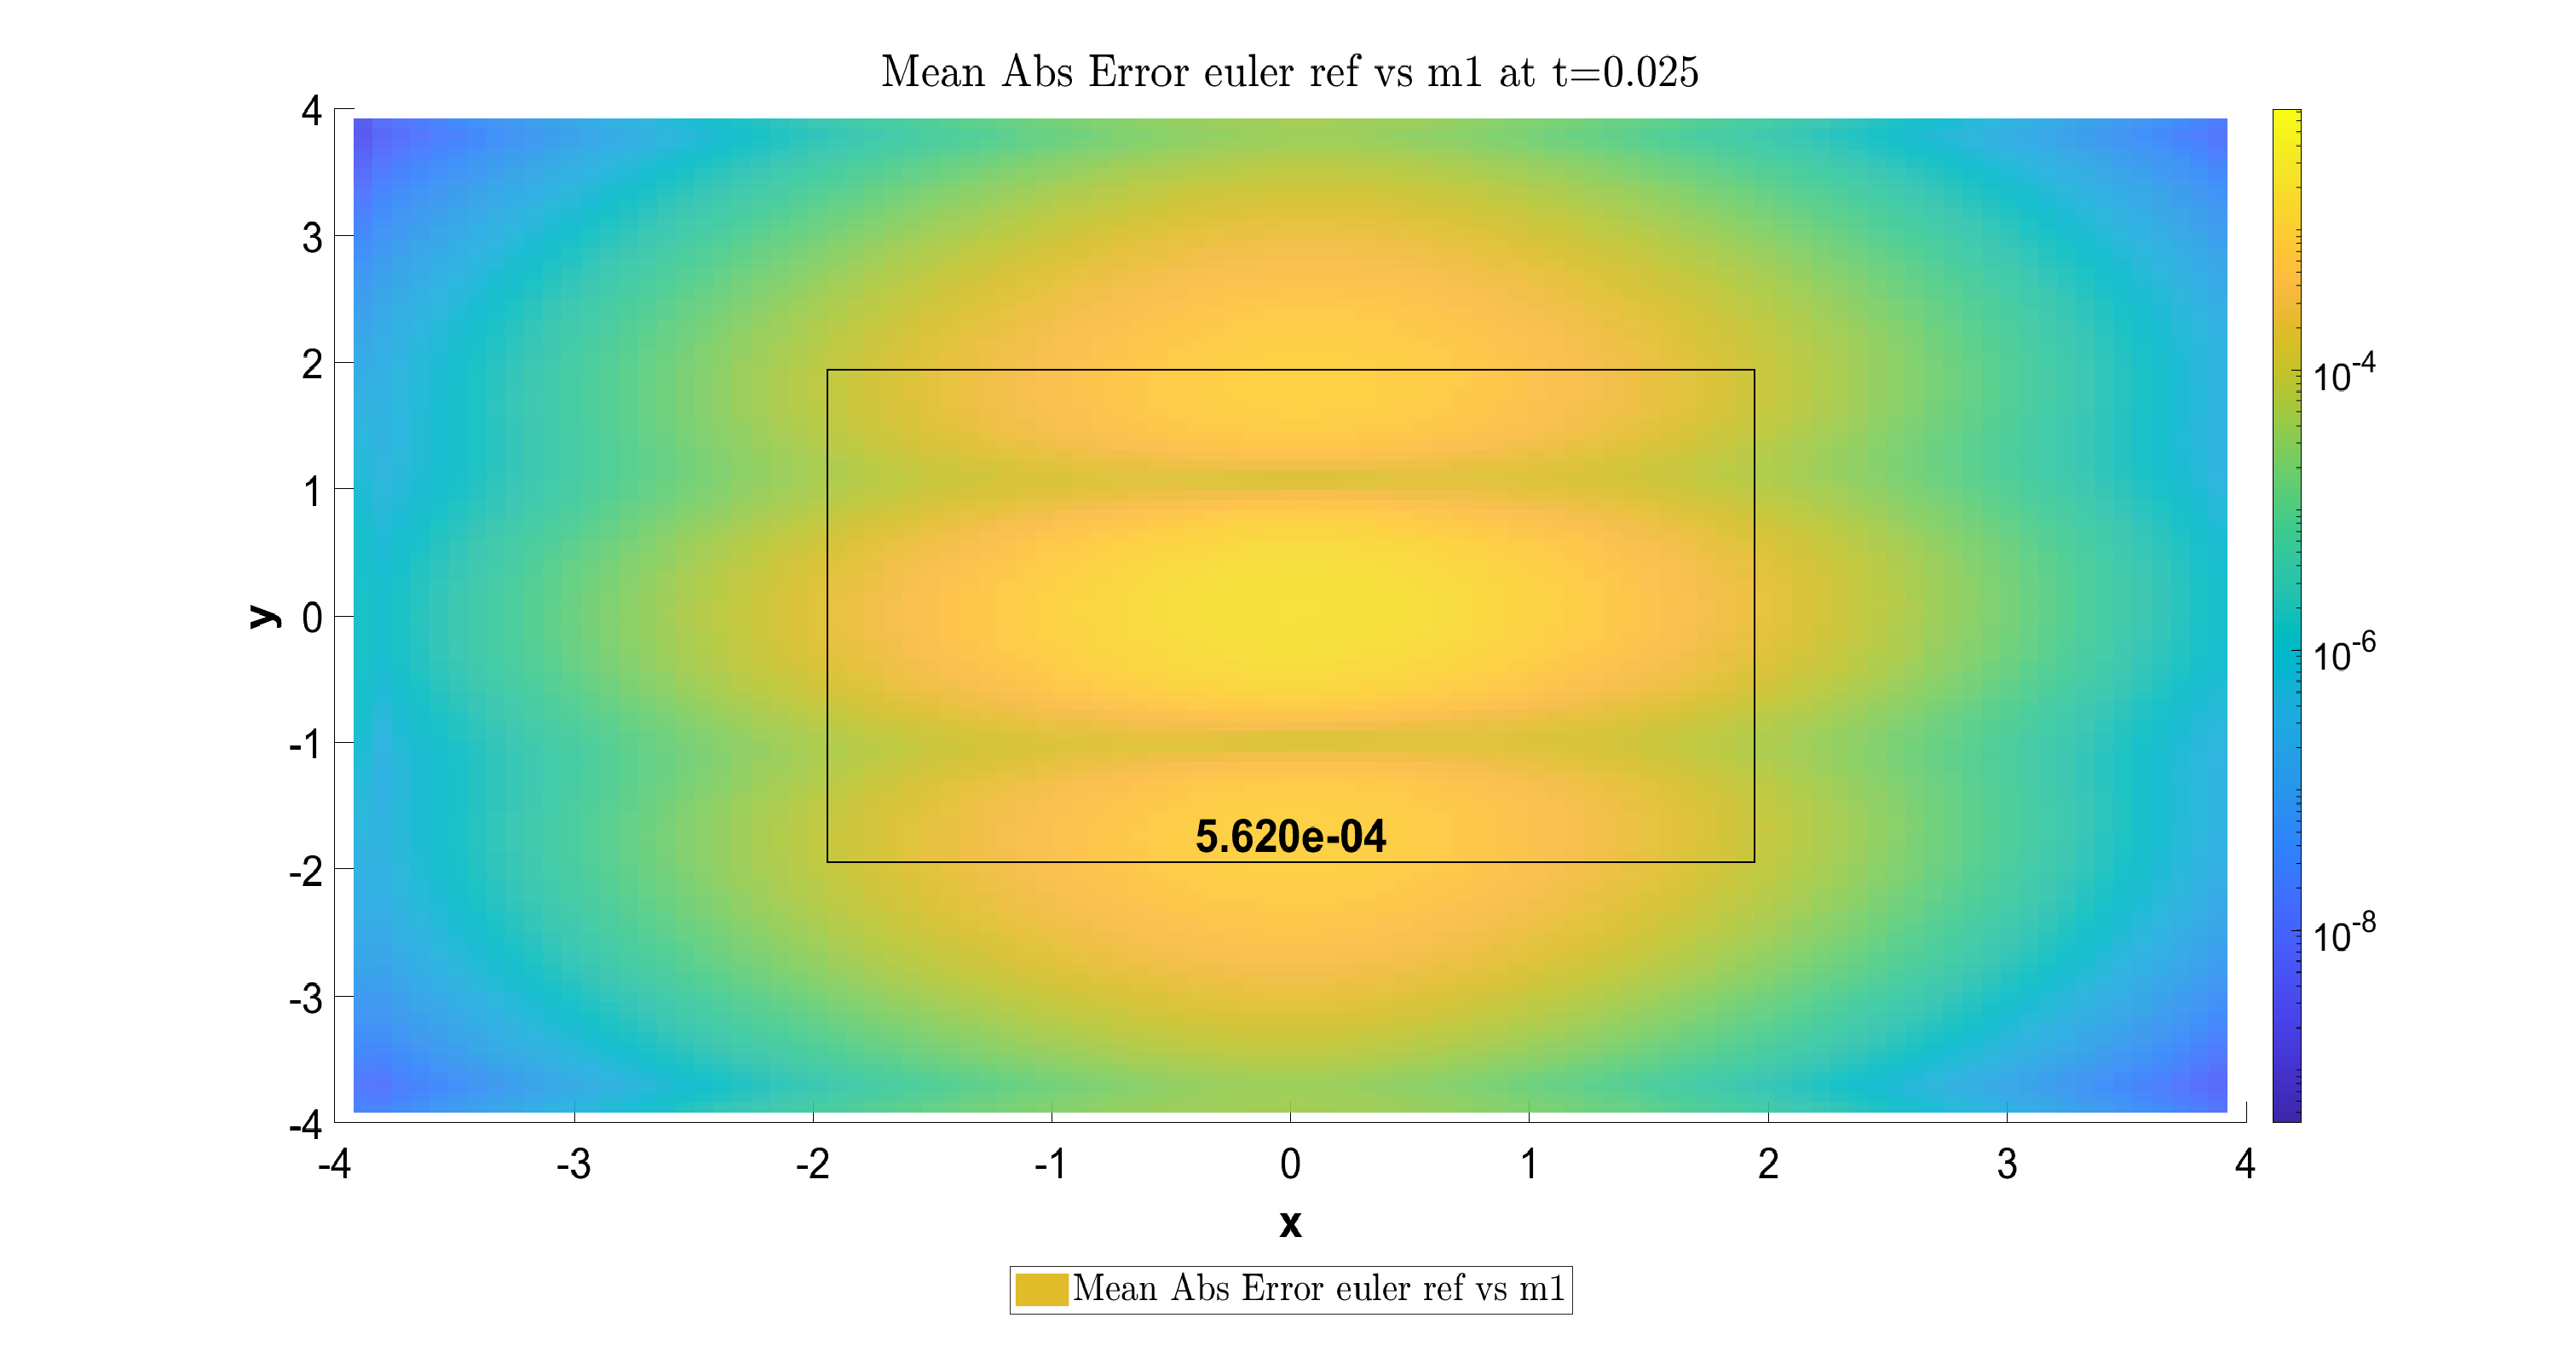
\includegraphics[width=.95\columnwidth]{CDF/CDFEulerRef_1}
\end{landscape}
\begin{landscape}
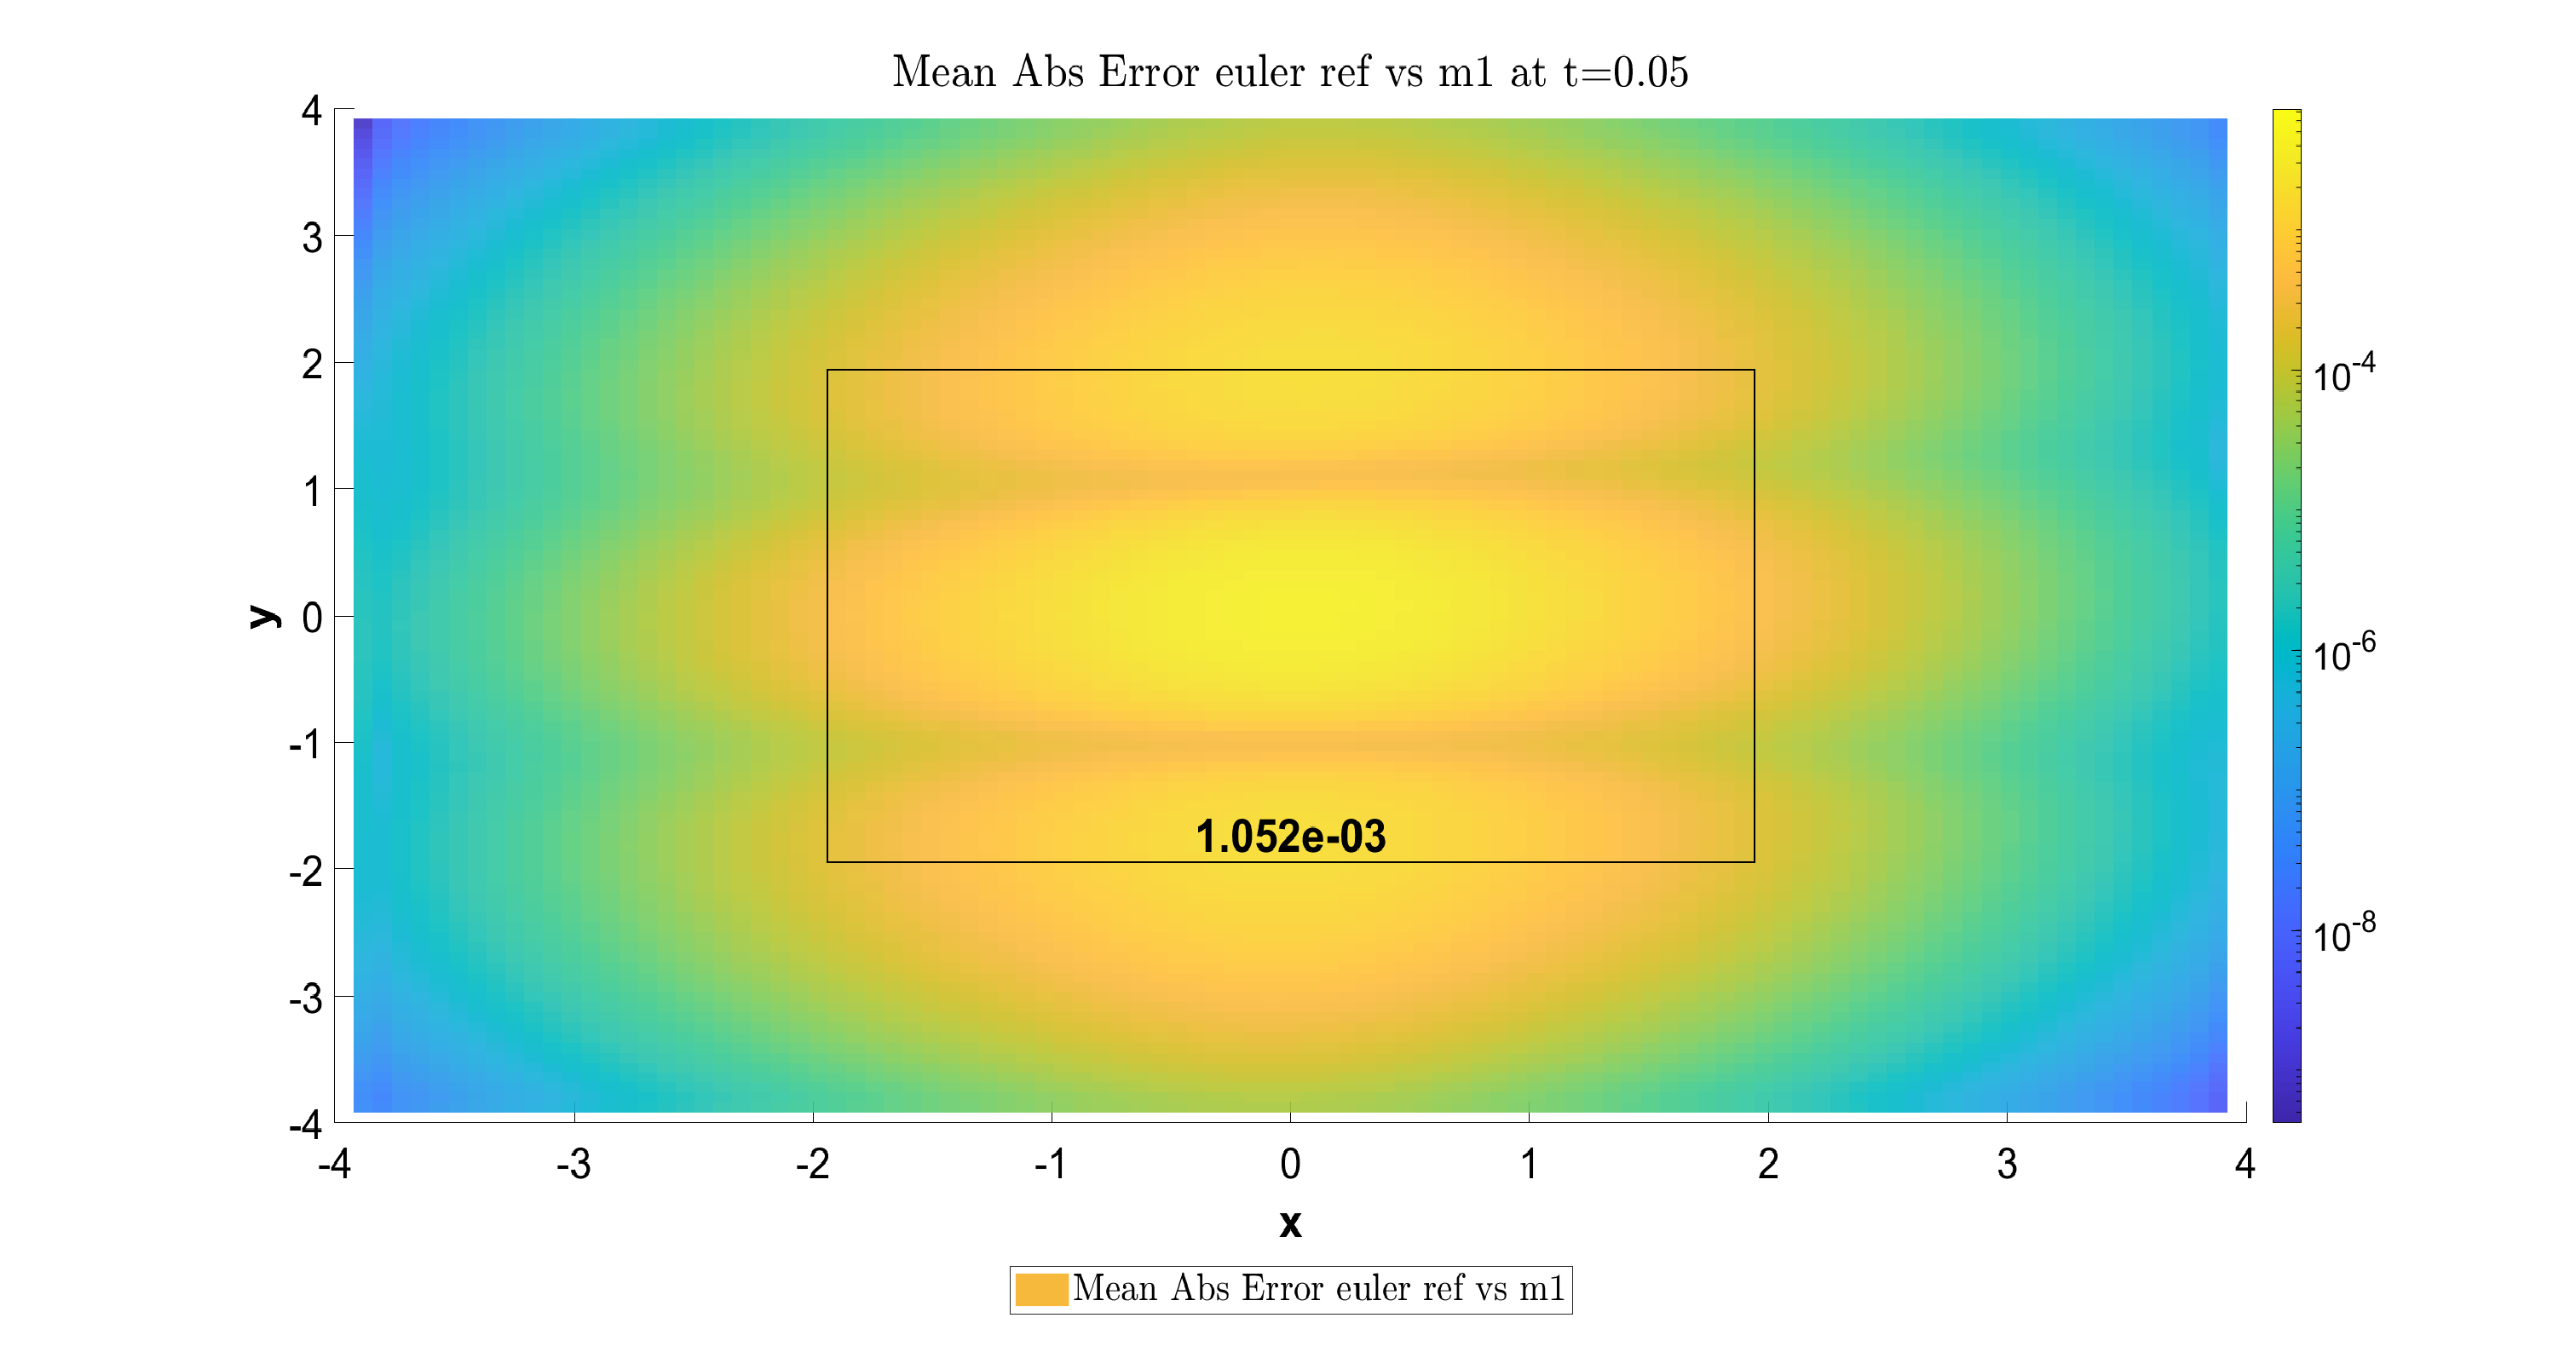
\includegraphics[width=.95\columnwidth]{CDF/CDFEulerRef_2}
\end{landscape}
\begin{landscape}
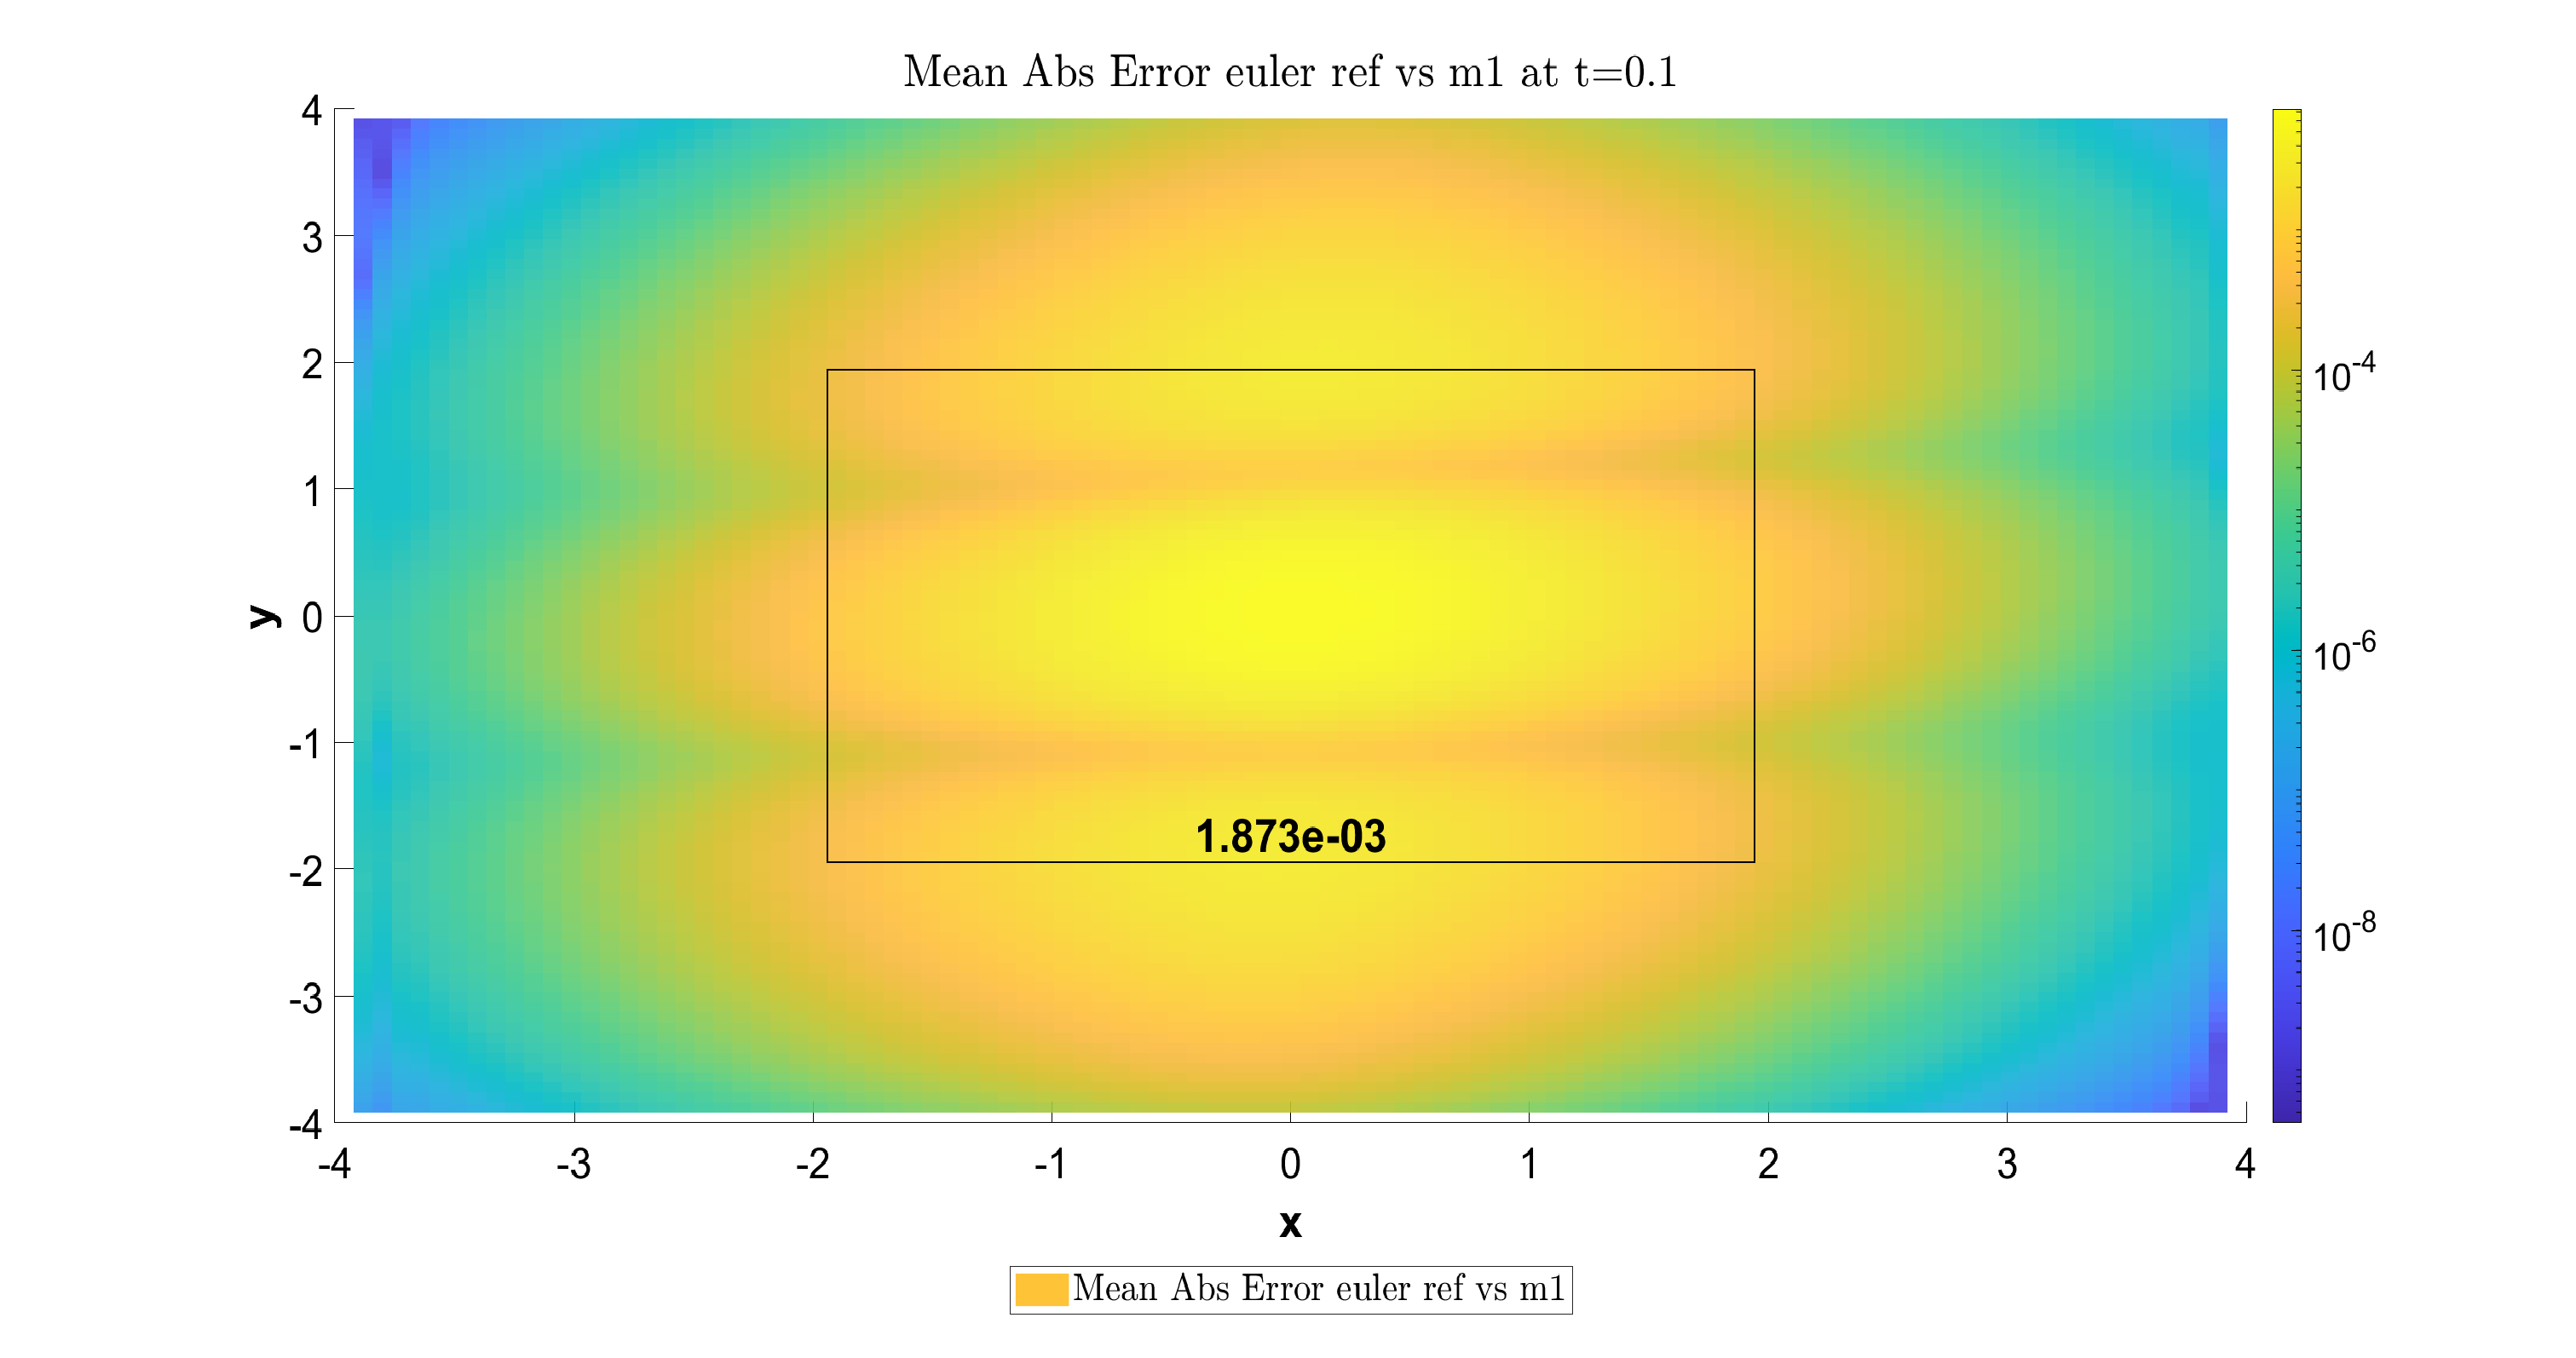
\includegraphics[width=.95\columnwidth]{CDF/CDFEulerRef_3}
\end{landscape}
\begin{landscape}
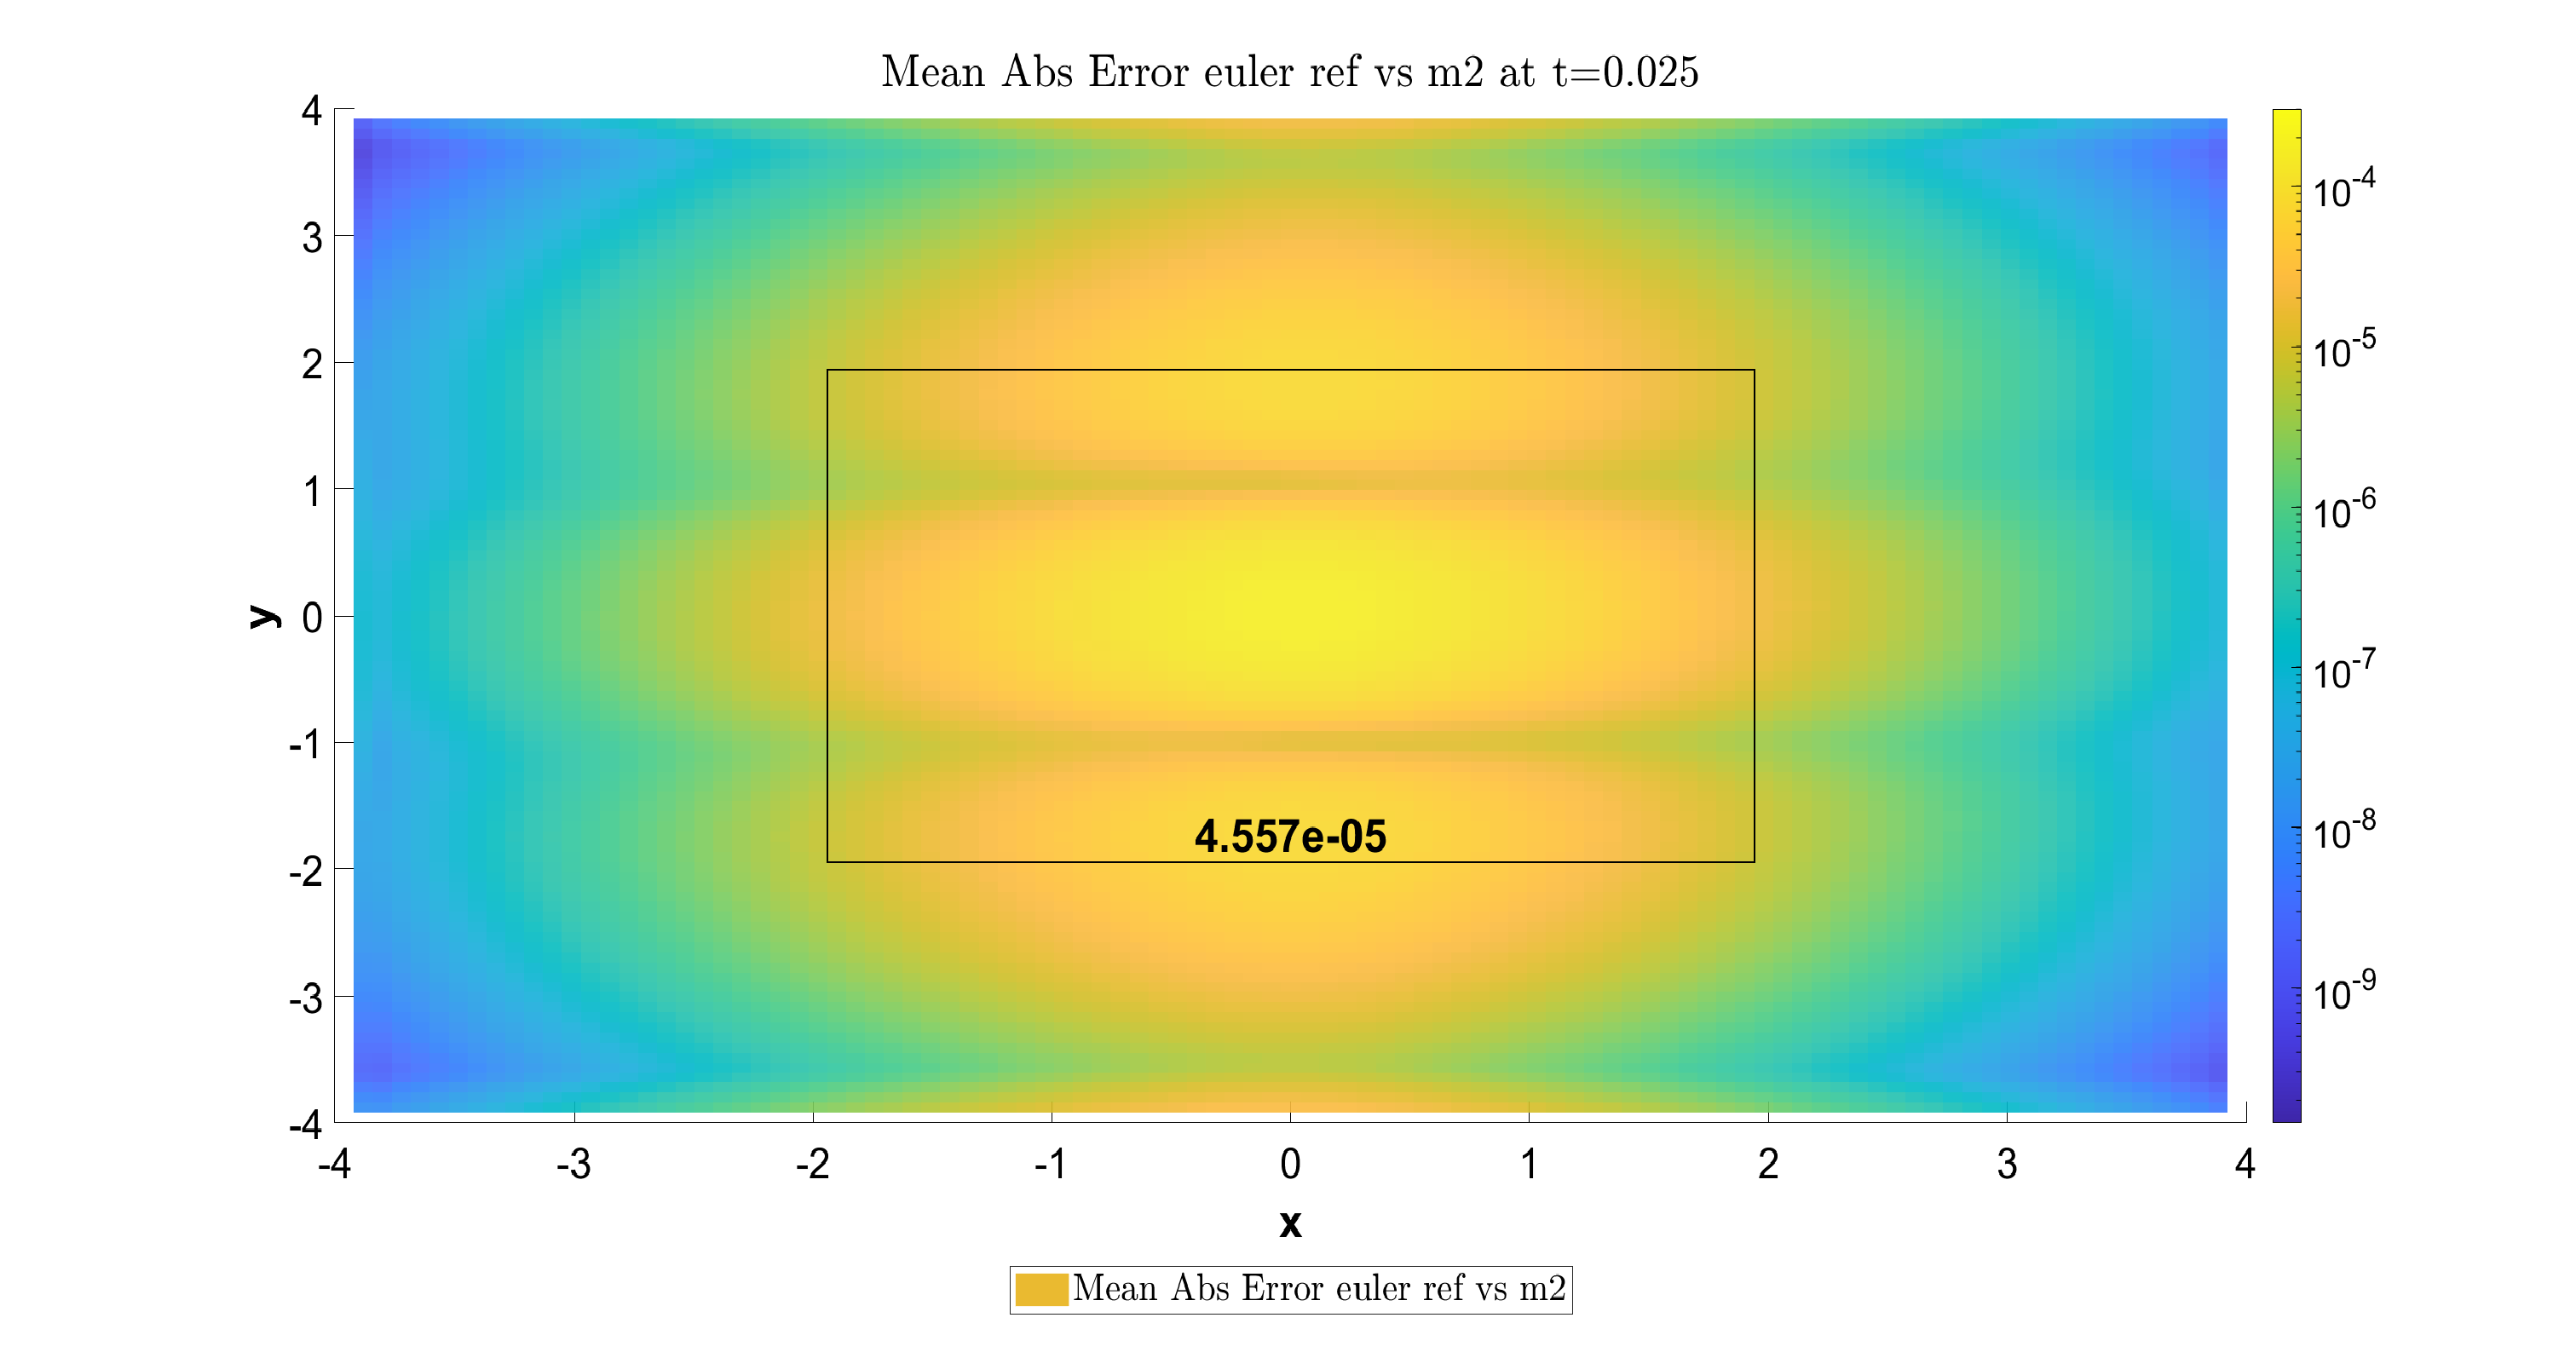
\includegraphics[width=.95\columnwidth]{CDF/CDFEulerRef_4}
\end{landscape}
\begin{landscape}
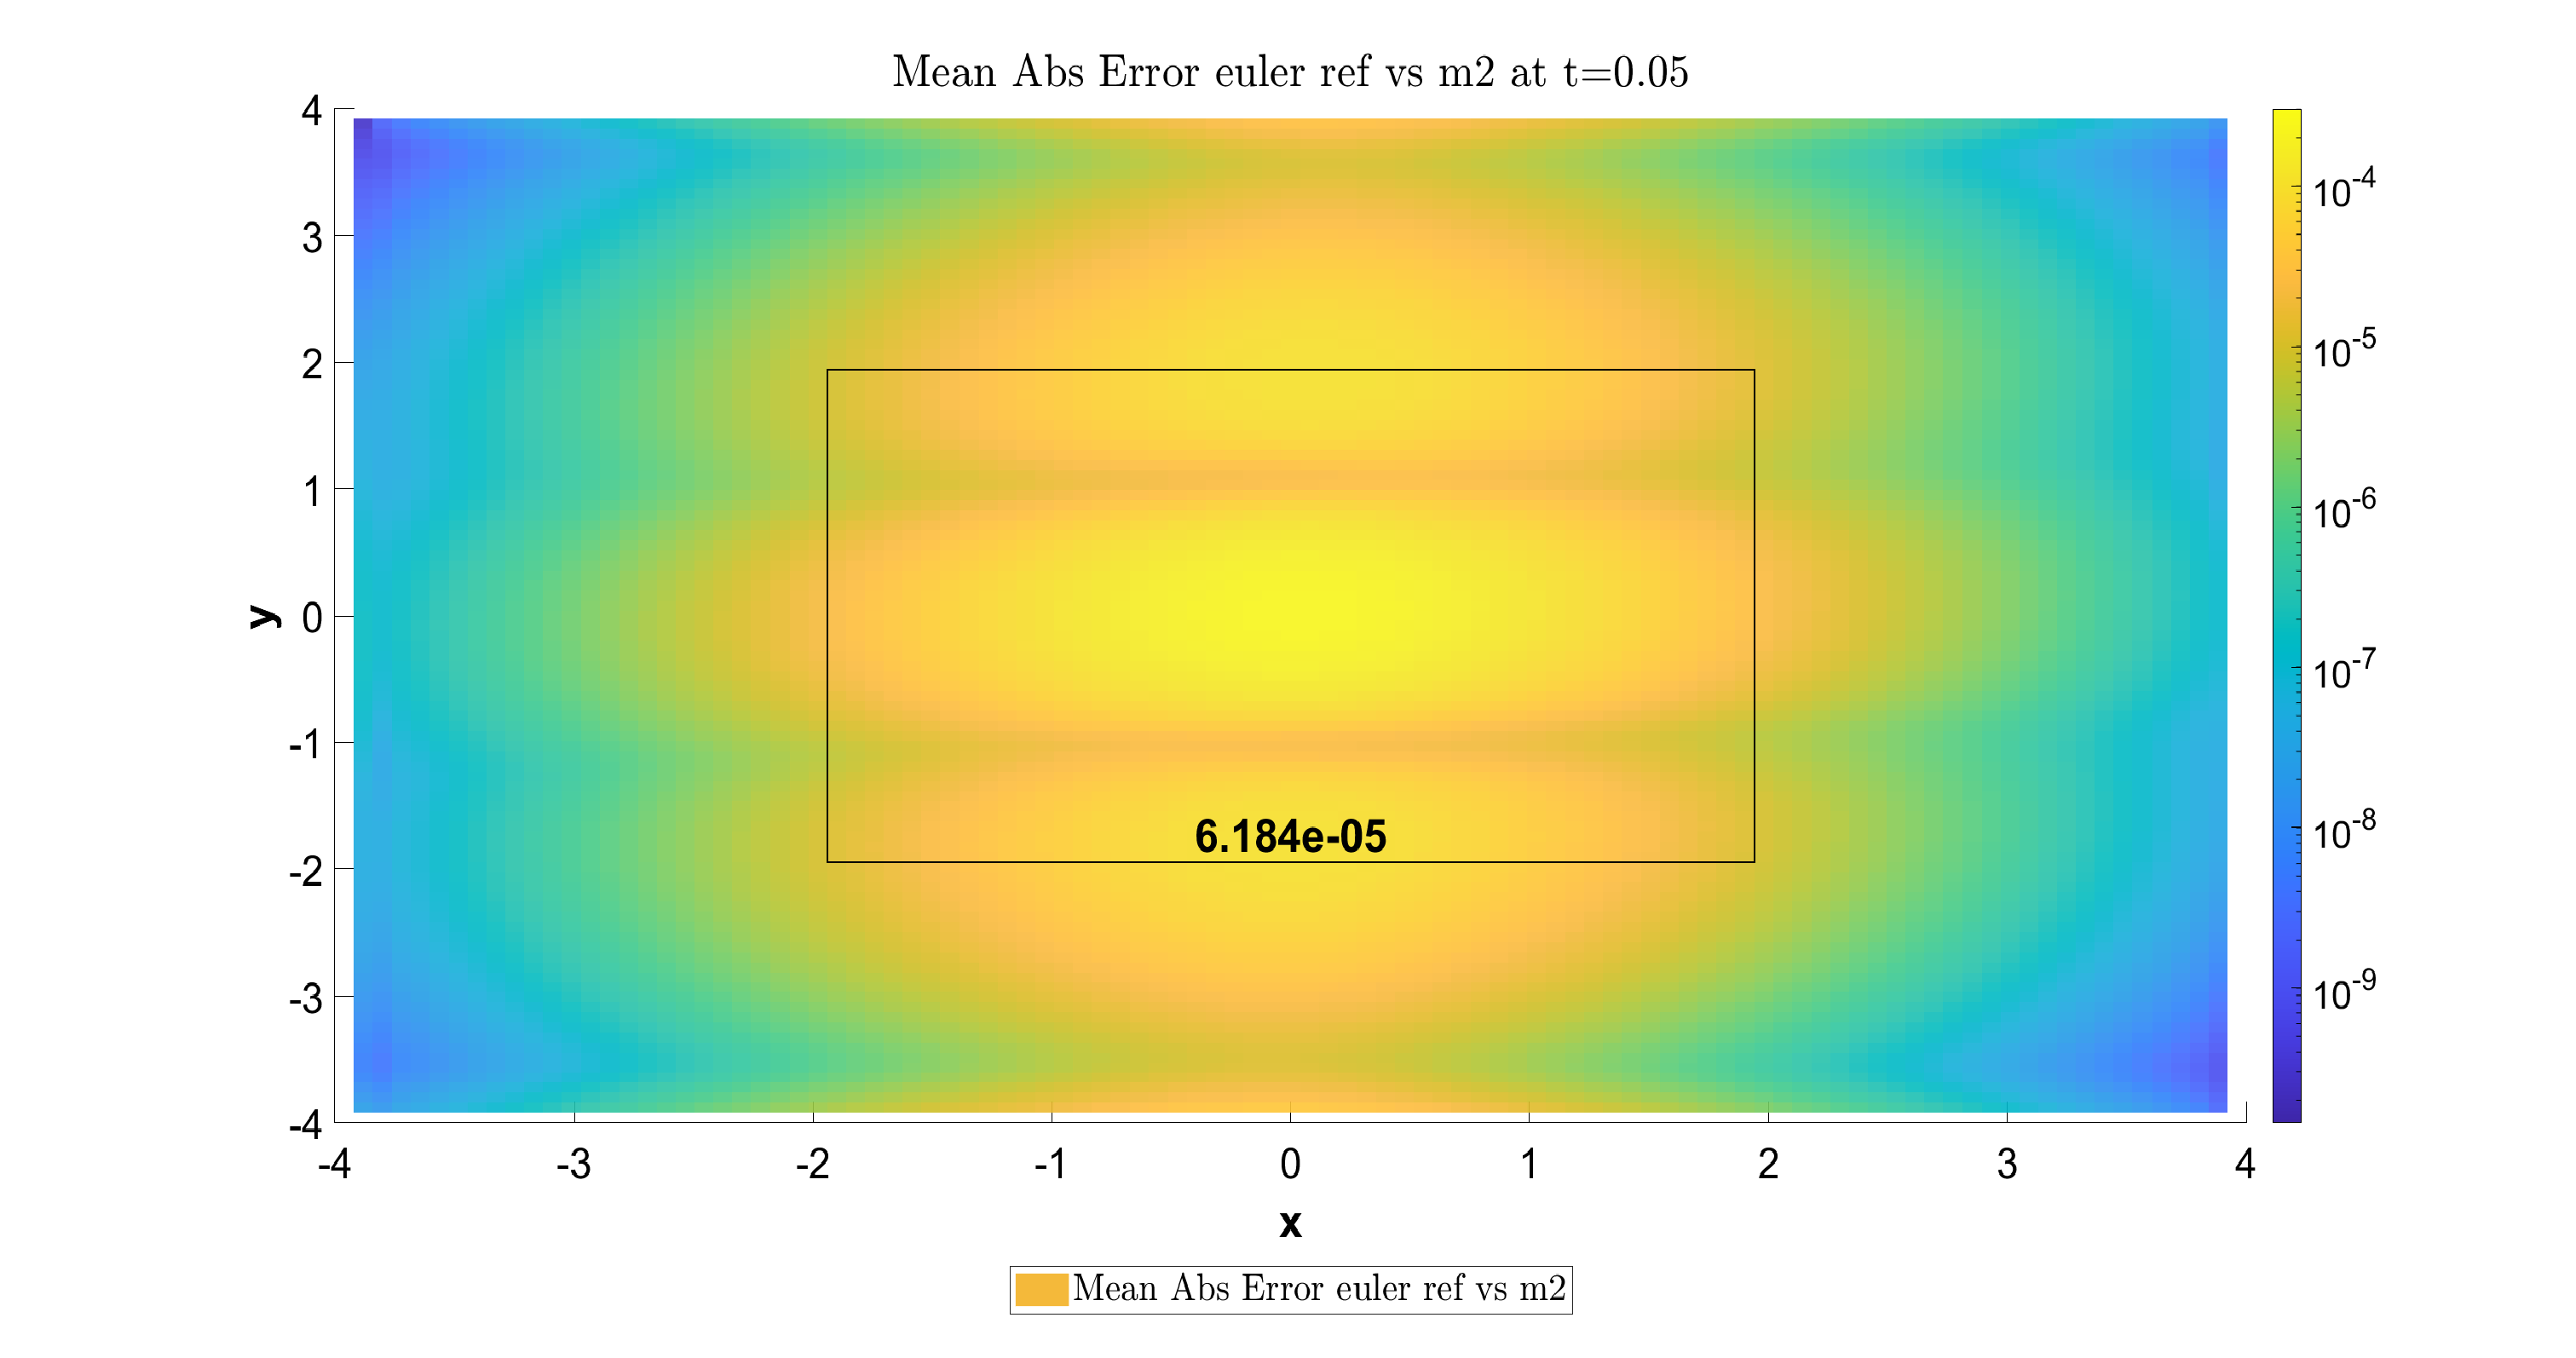
\includegraphics[width=.95\columnwidth]{CDF/CDFEulerRef_5}
\end{landscape}
\begin{landscape}
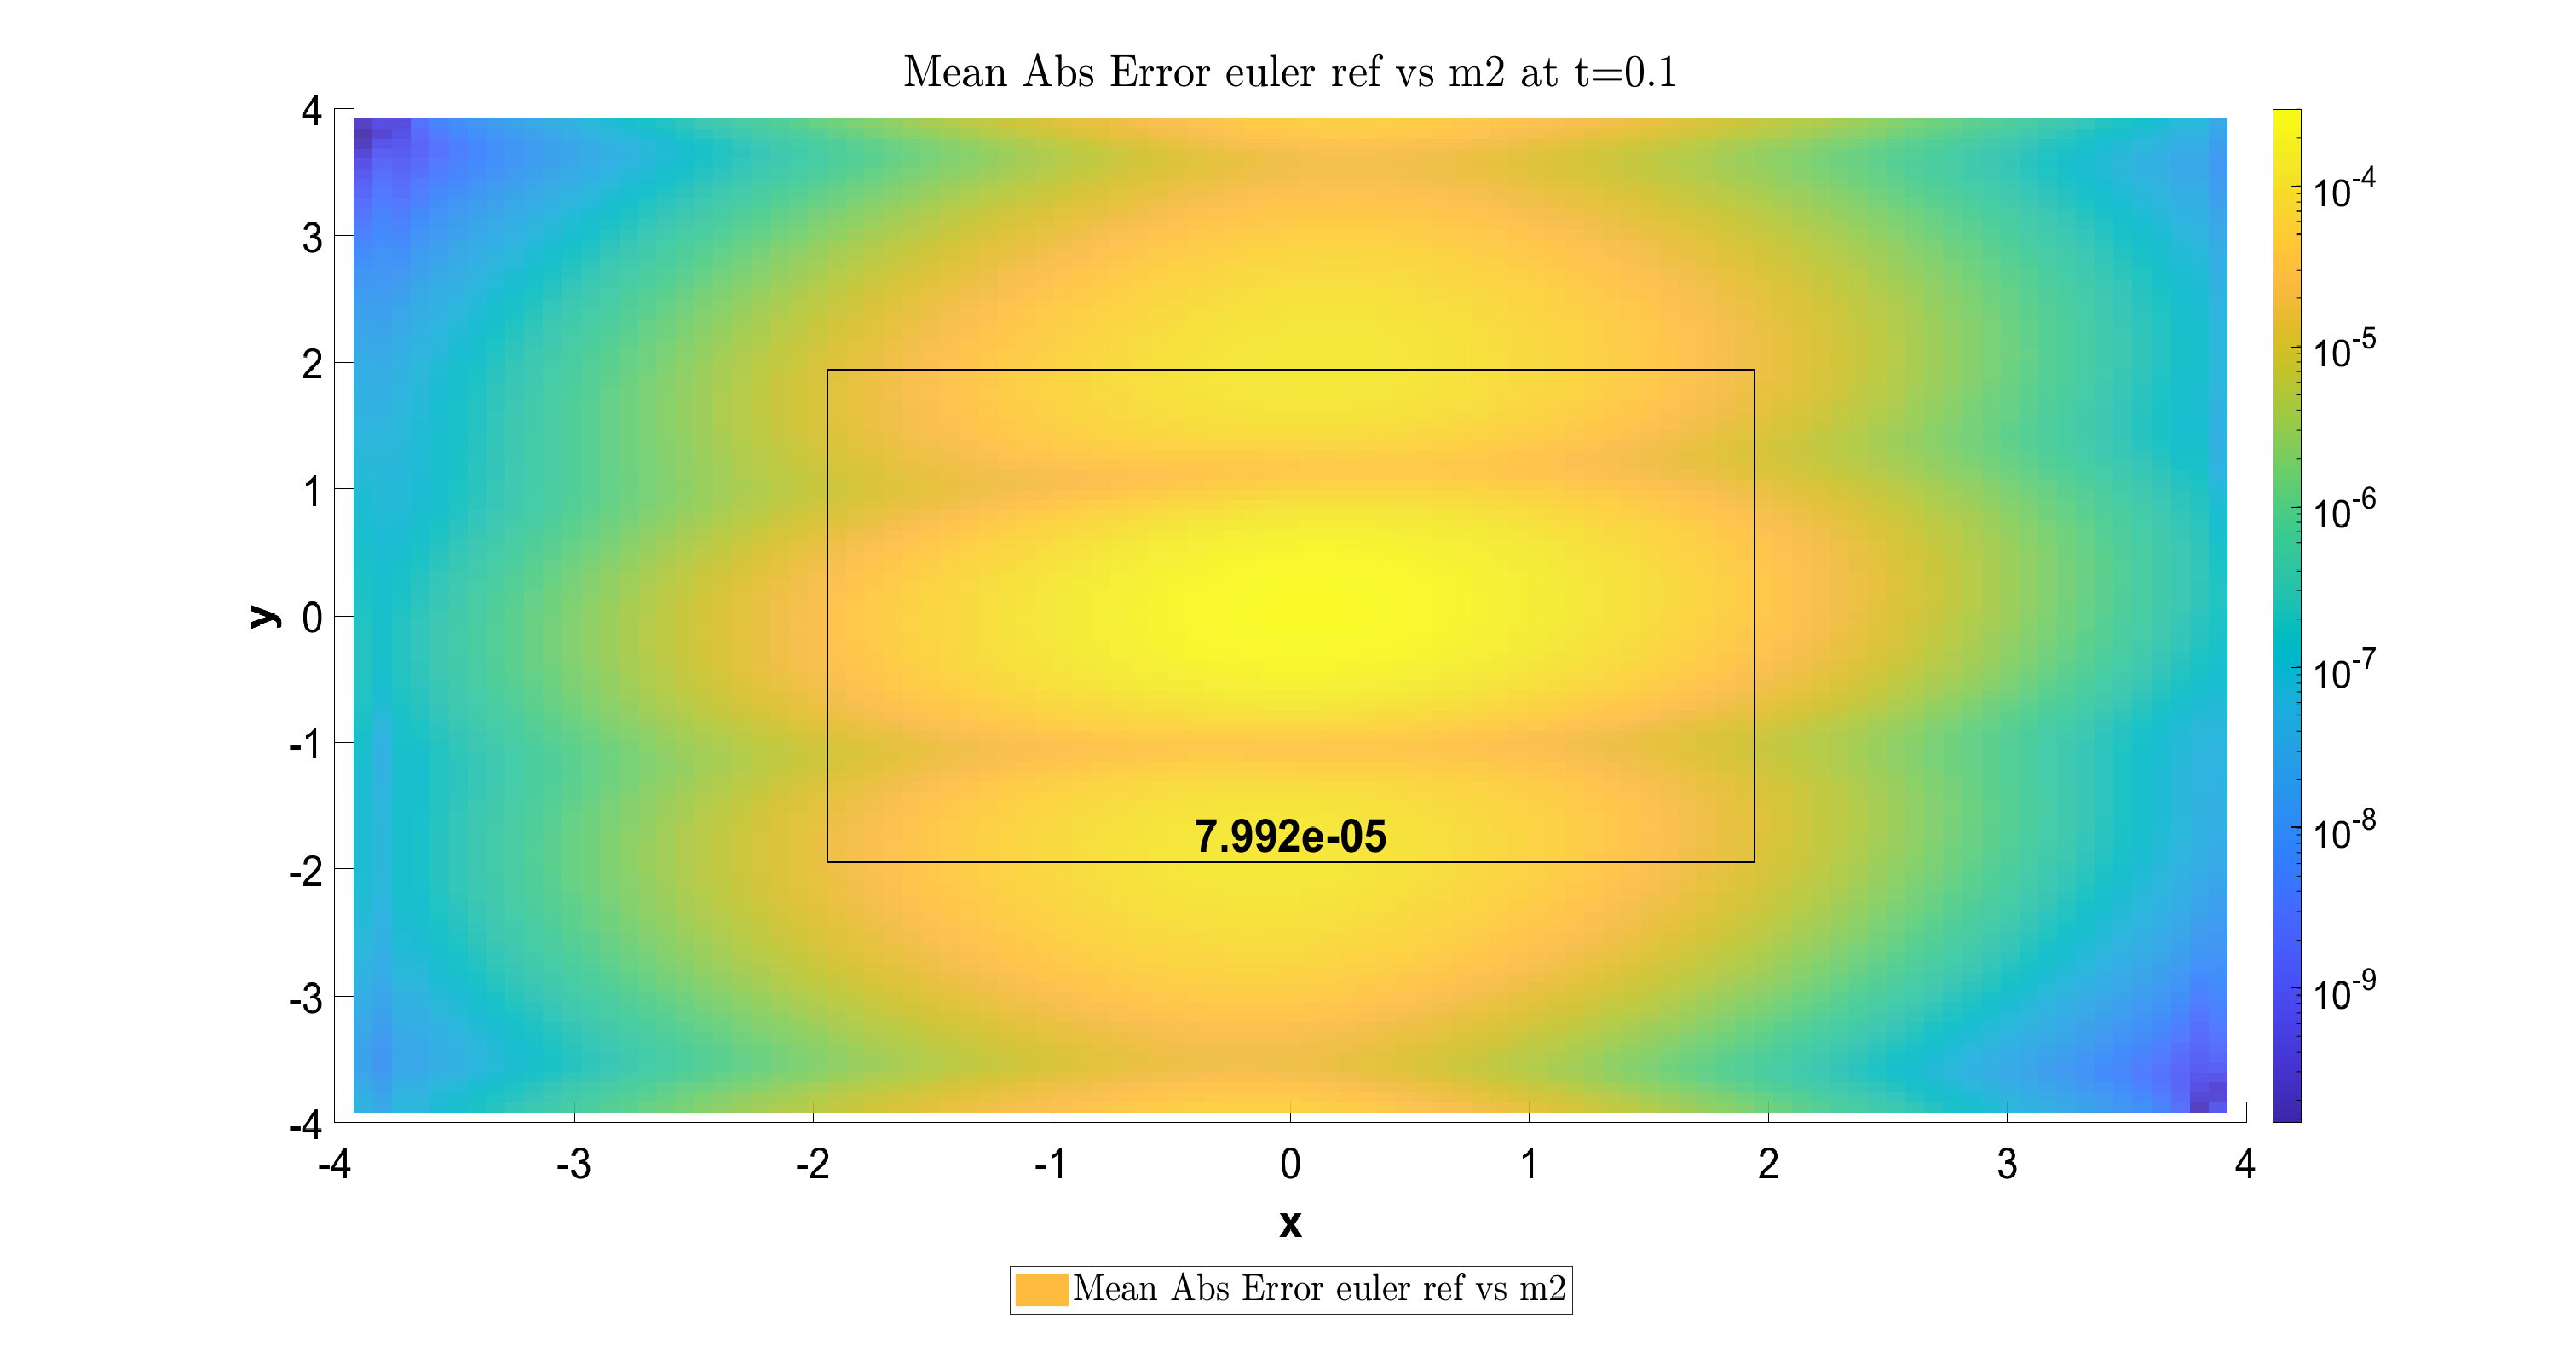
\includegraphics[width=.95\columnwidth]{CDF/CDFEulerRef_6}
\end{landscape}
\begin{landscape}
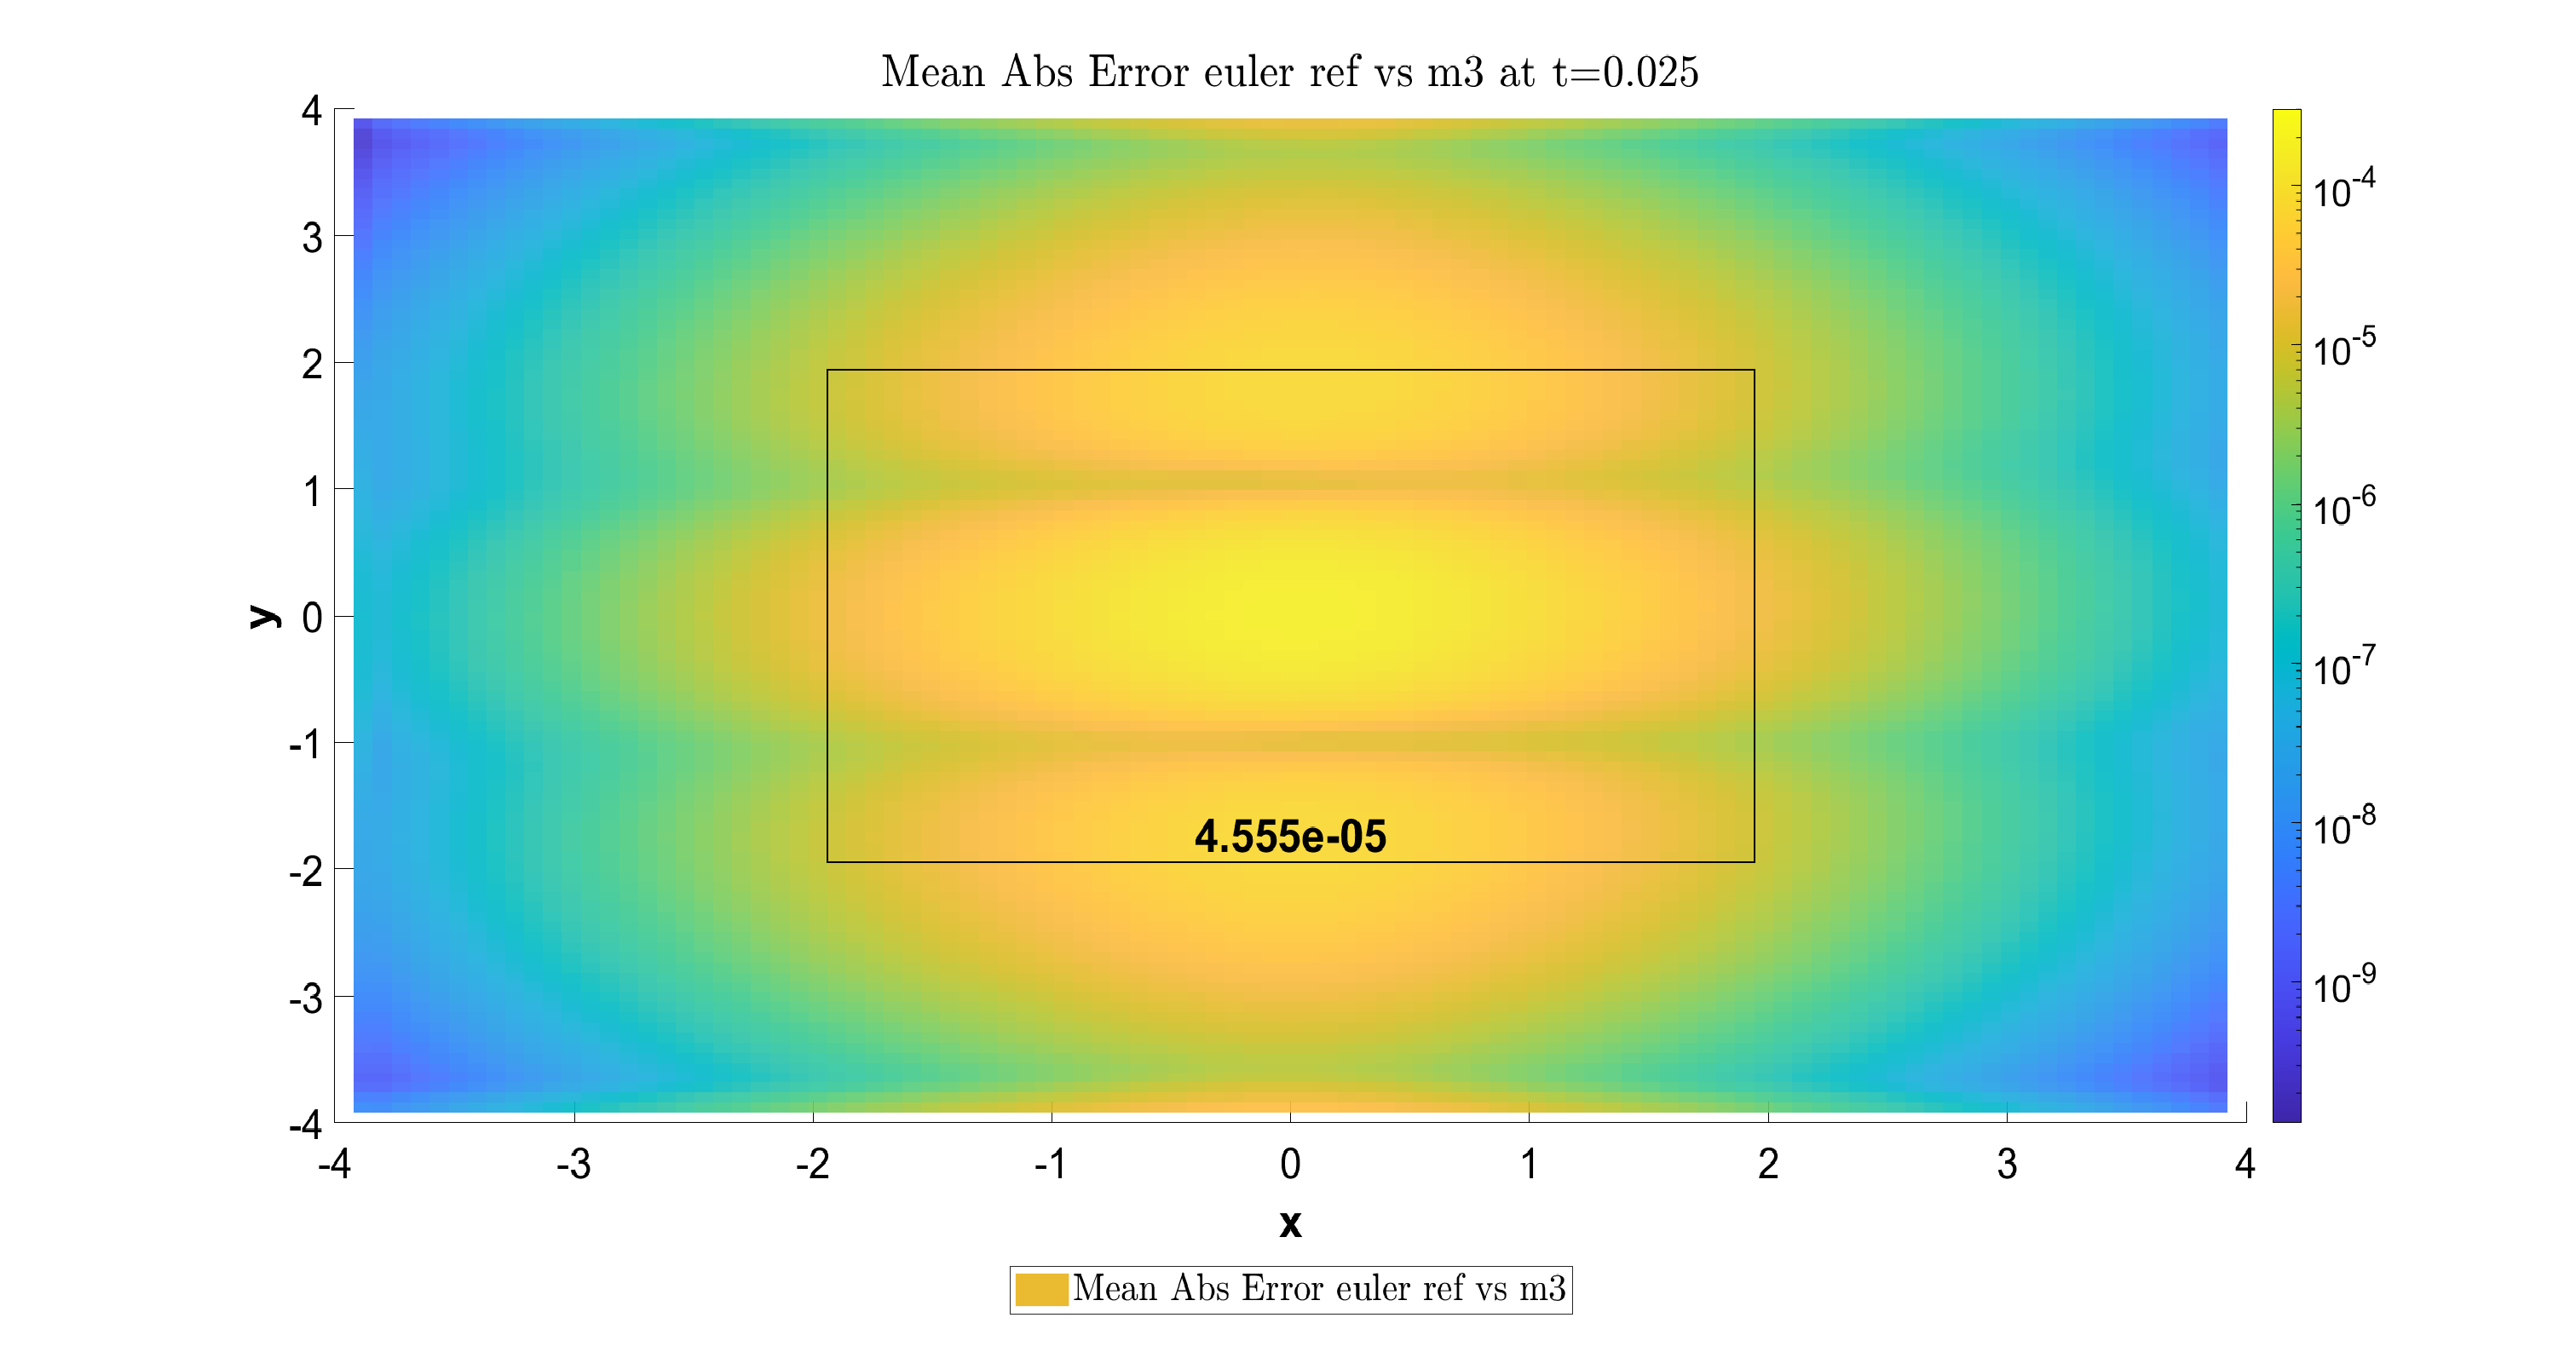
\includegraphics[width=.95\columnwidth]{CDF/CDFEulerRef_7}
\end{landscape}
\begin{landscape}
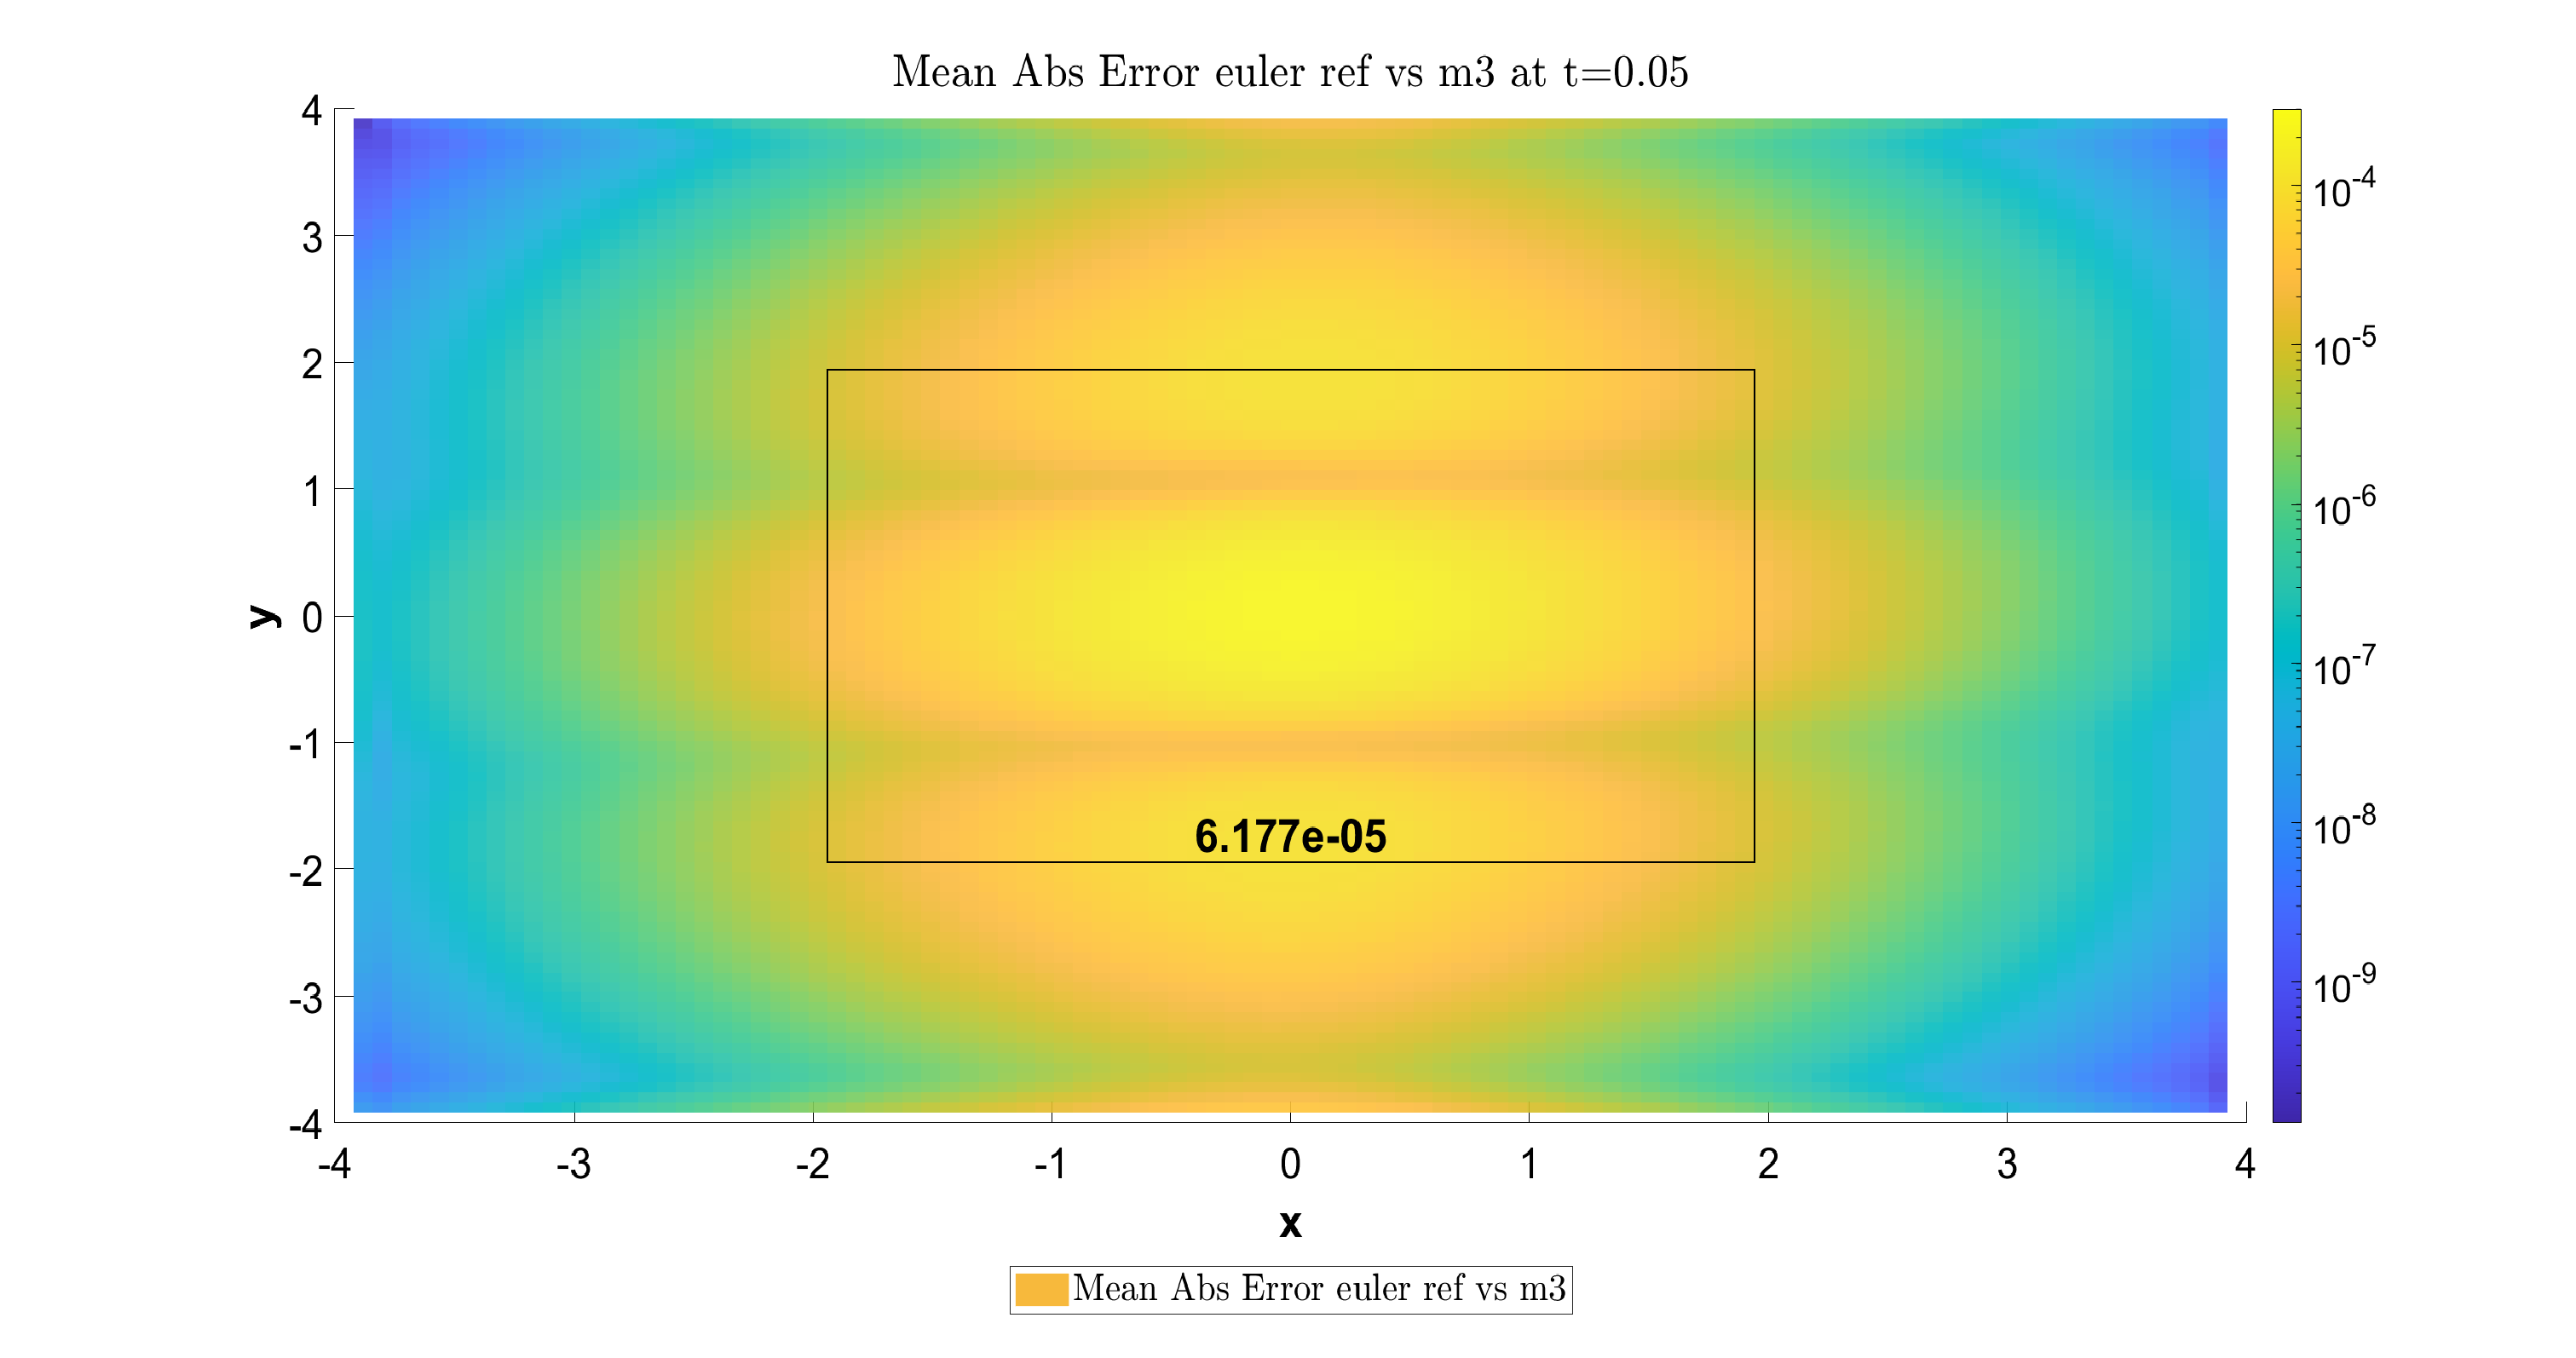
\includegraphics[width=.95\columnwidth]{CDF/CDFEulerRef_8}
\end{landscape}
\begin{landscape}
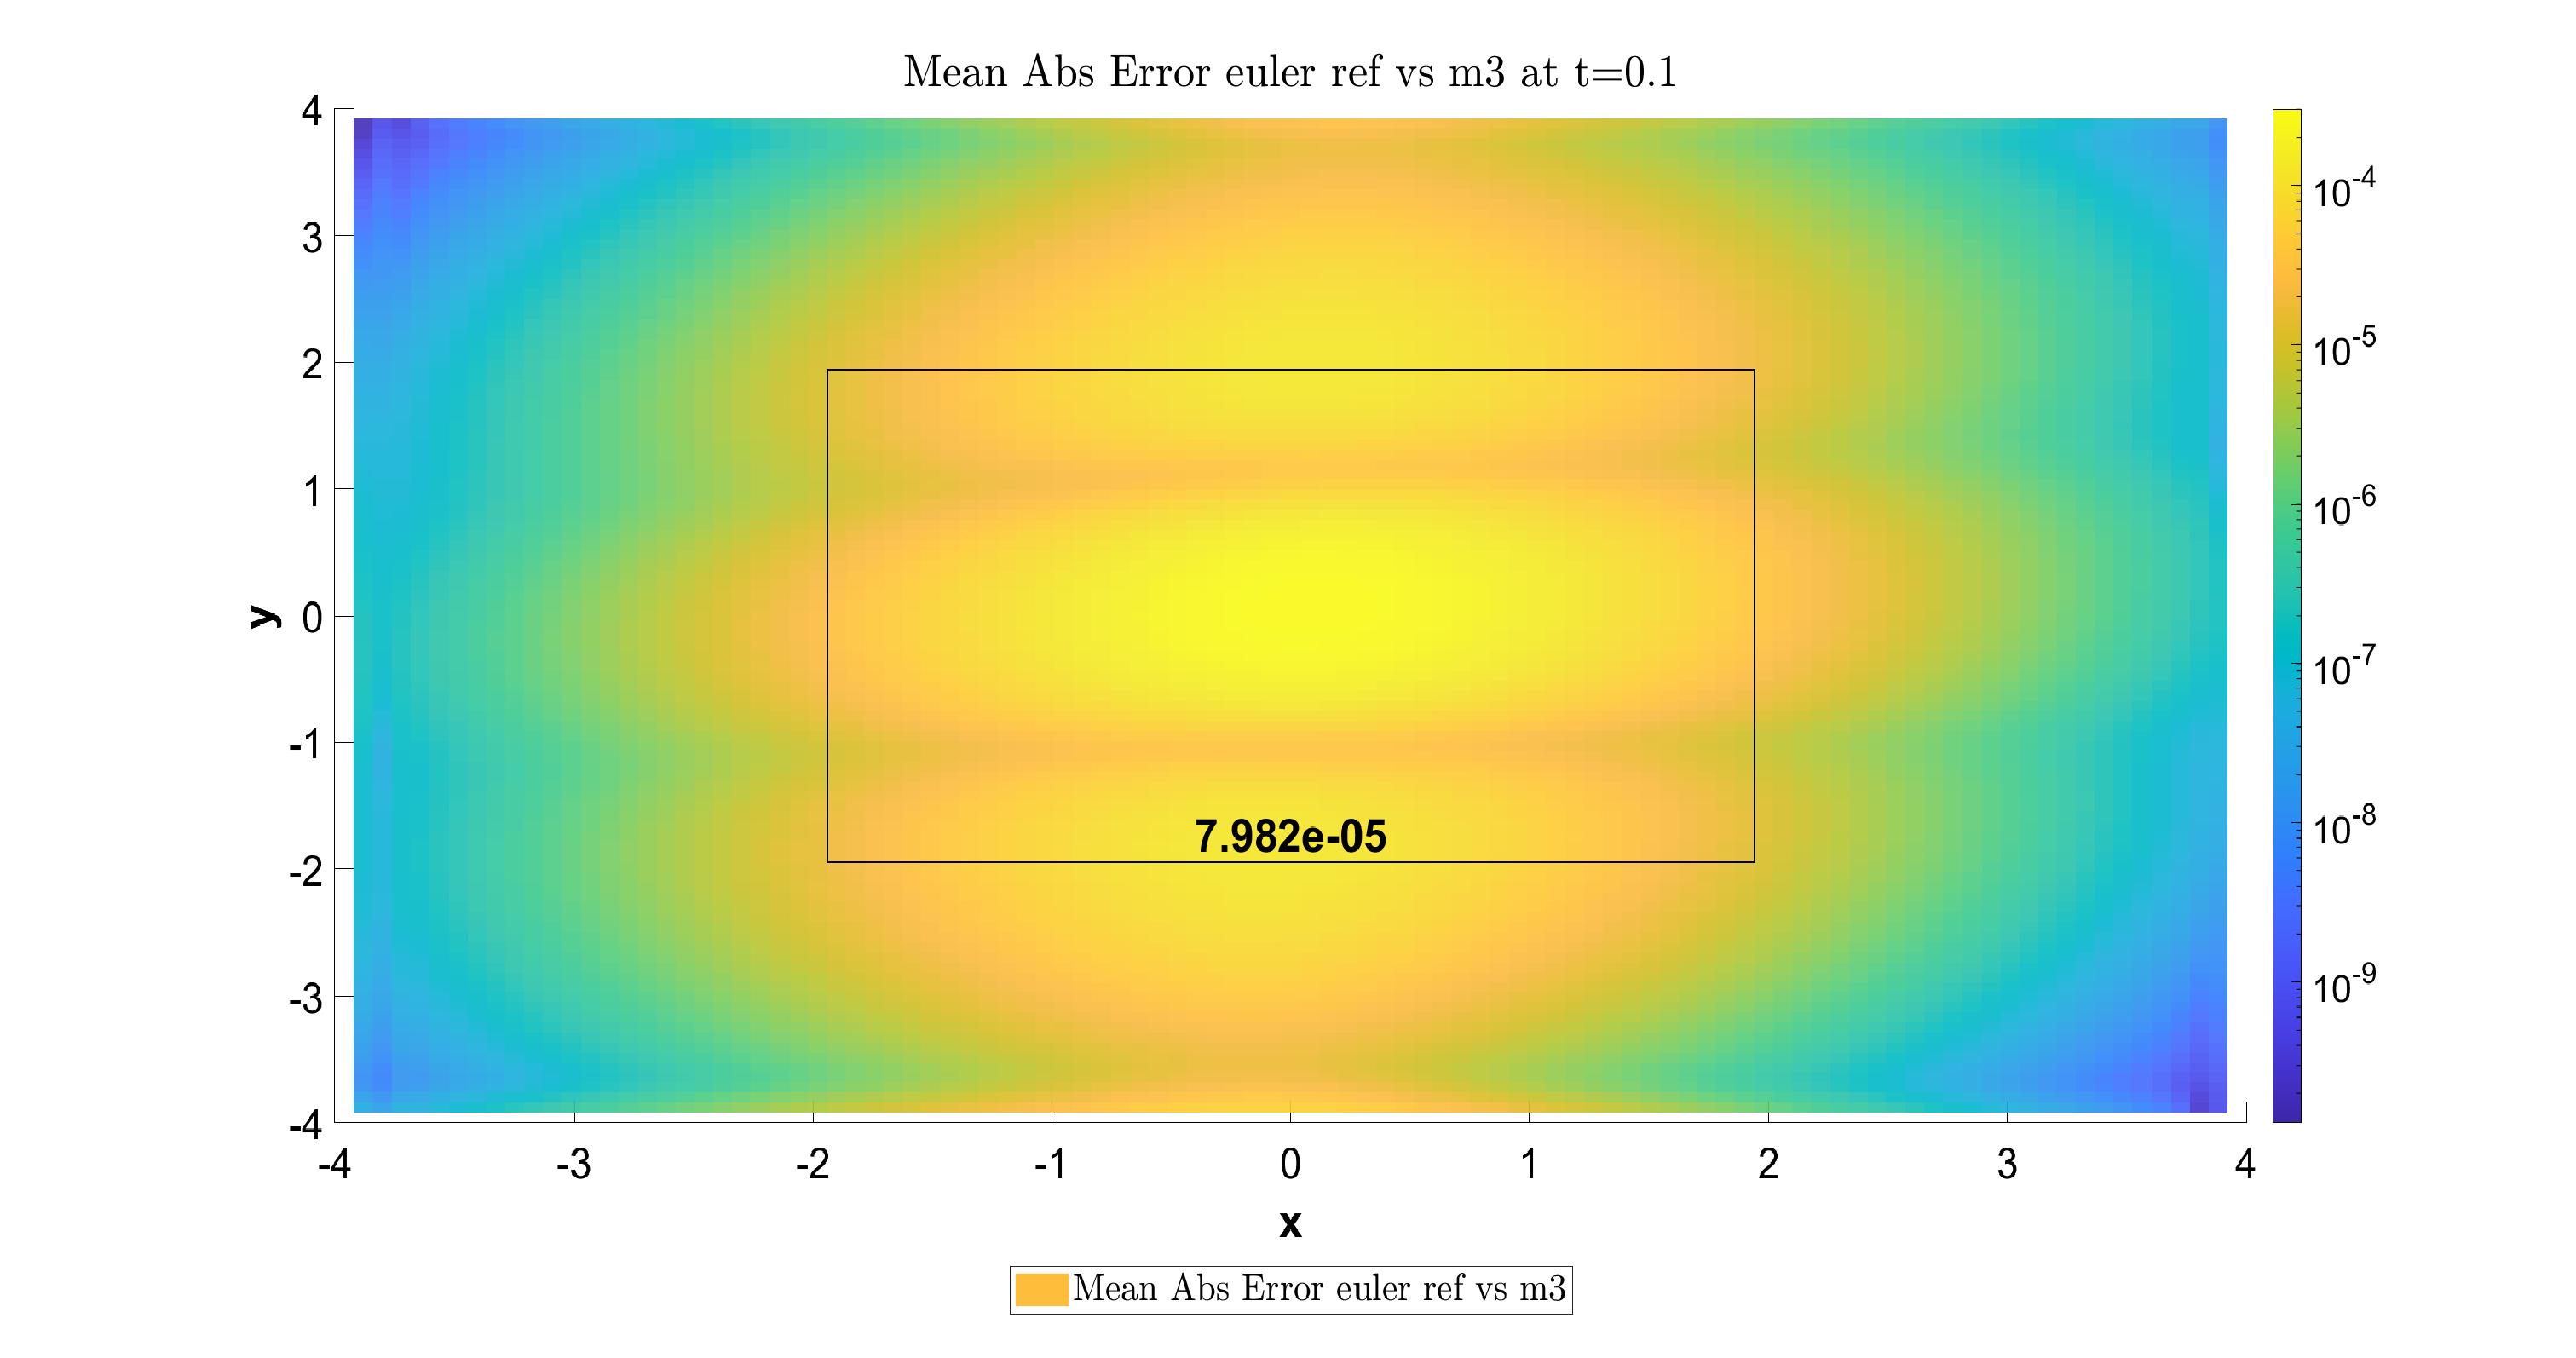
\includegraphics[width=.95\columnwidth]{CDF/CDFEulerRef_9}
\end{landscape}
\begin{landscape}
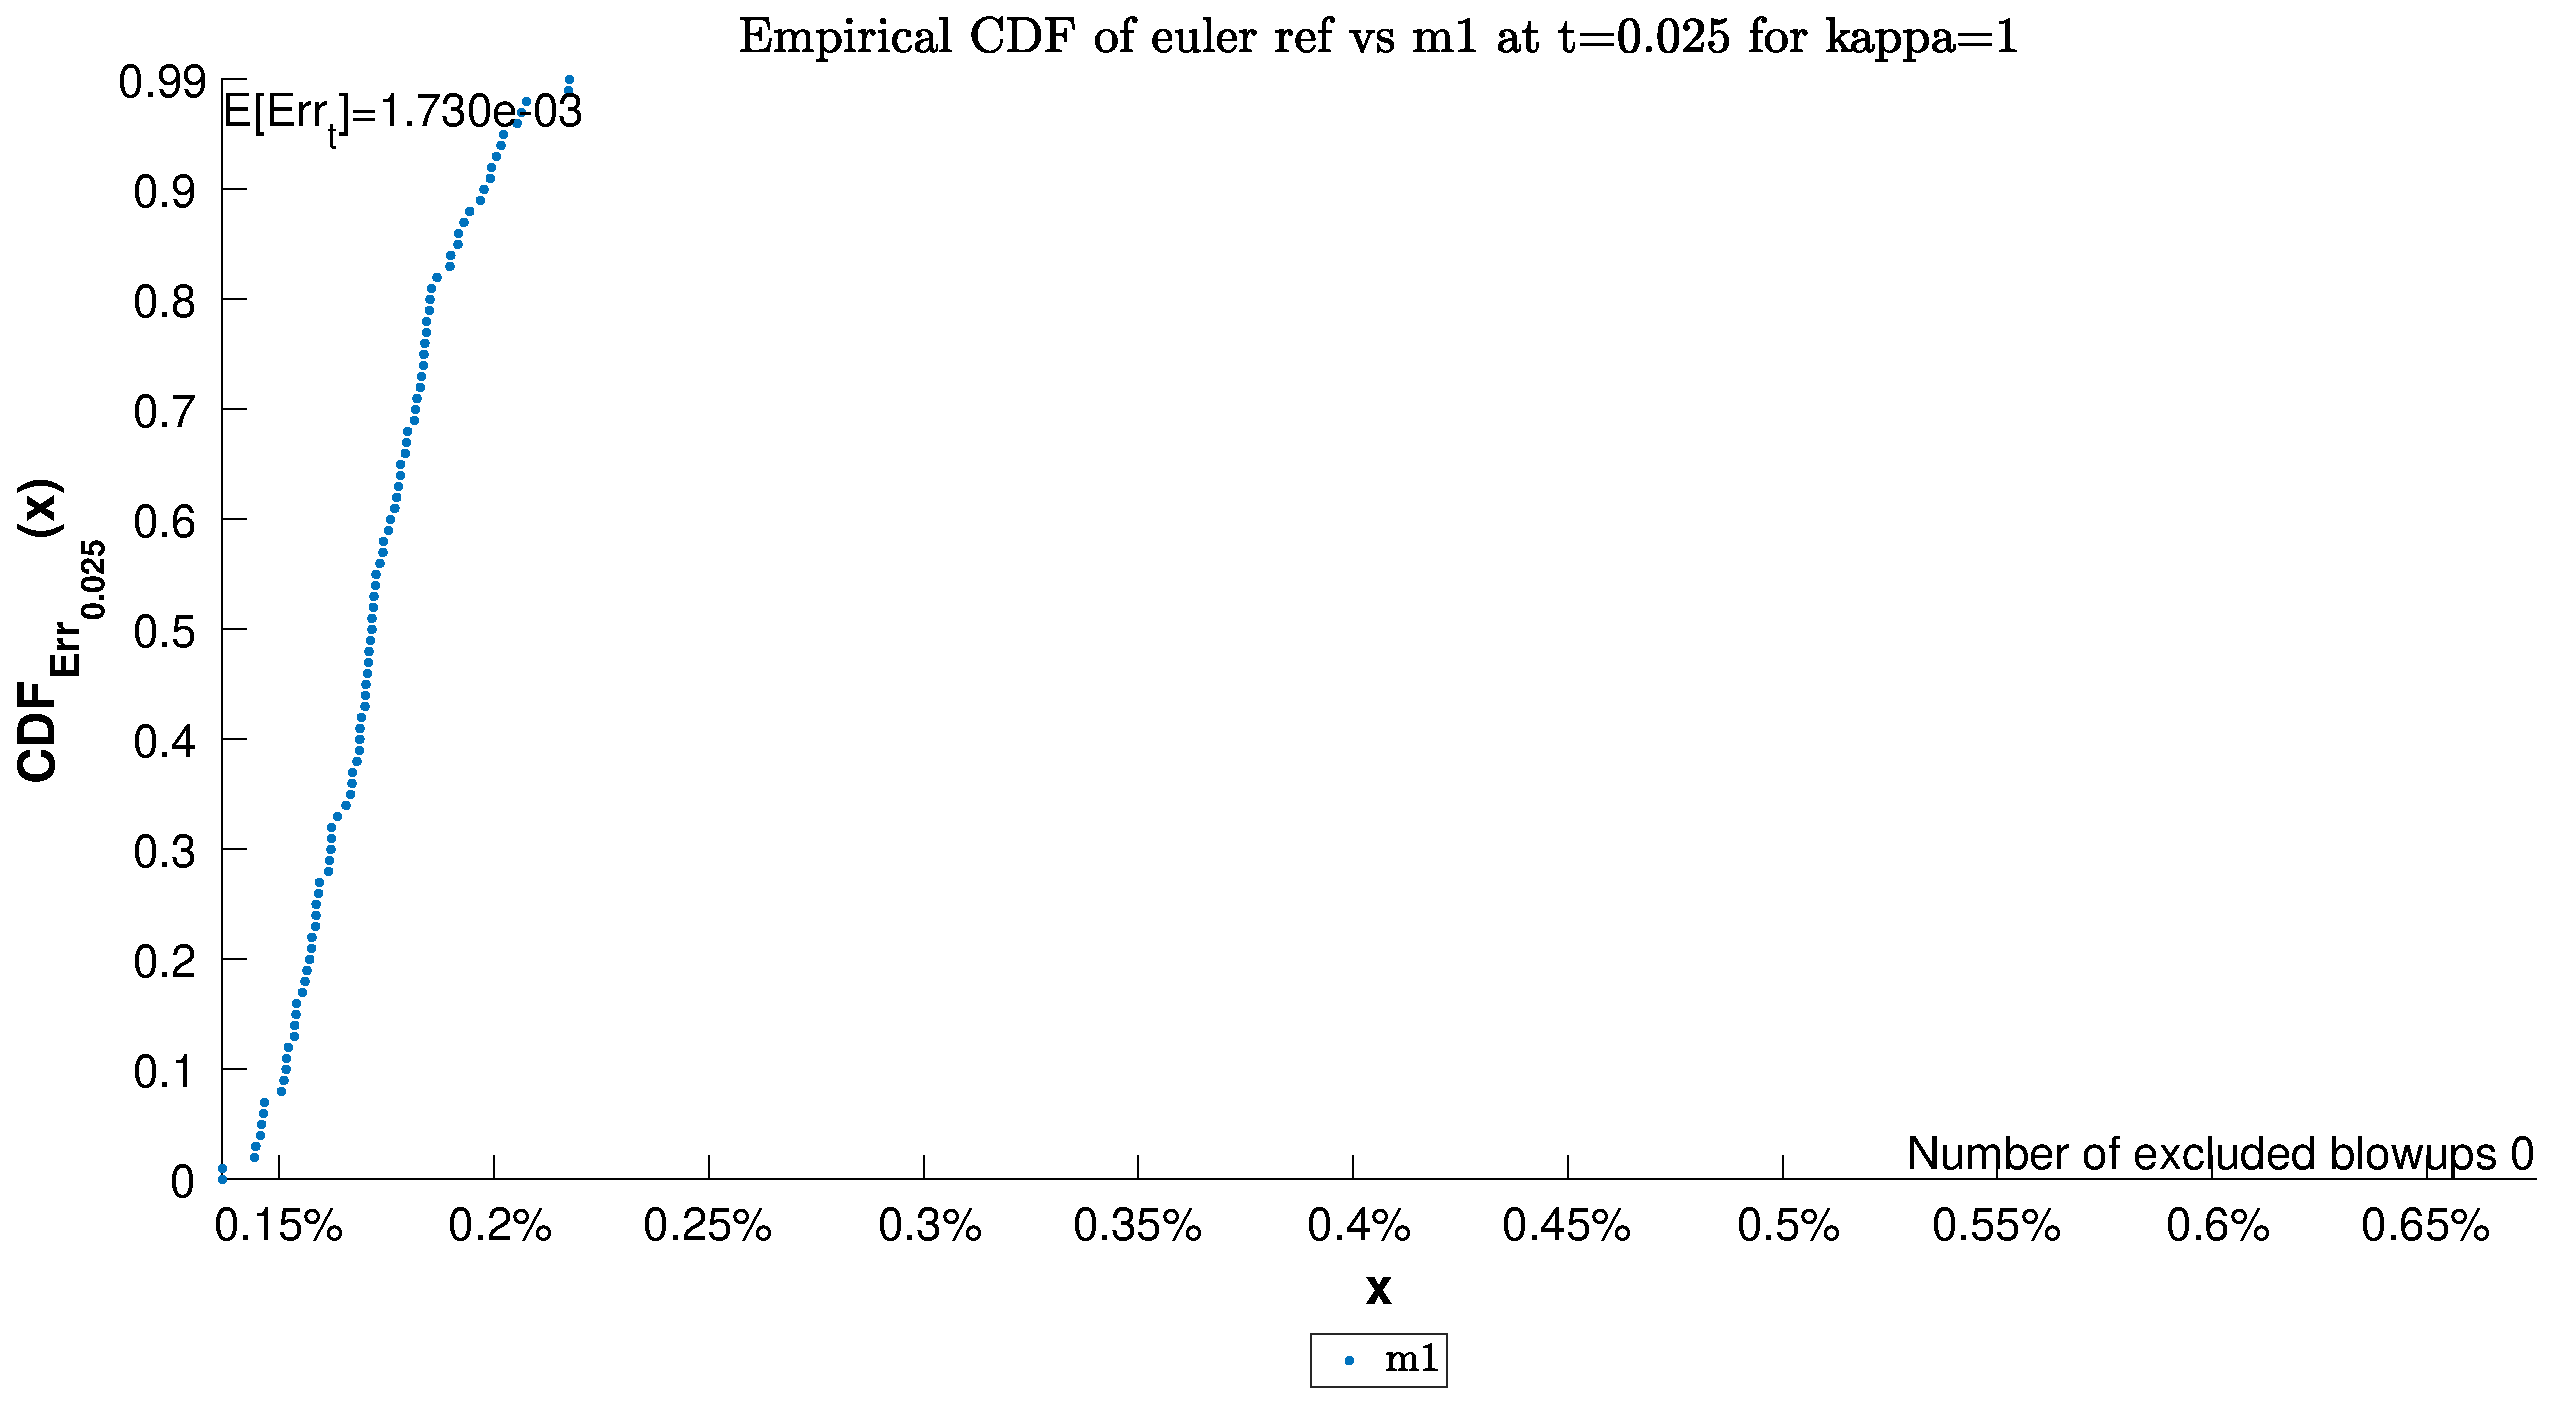
\includegraphics[width=.95\columnwidth]{CDF/CDFEulerRef_10}
\end{landscape}
\begin{landscape}
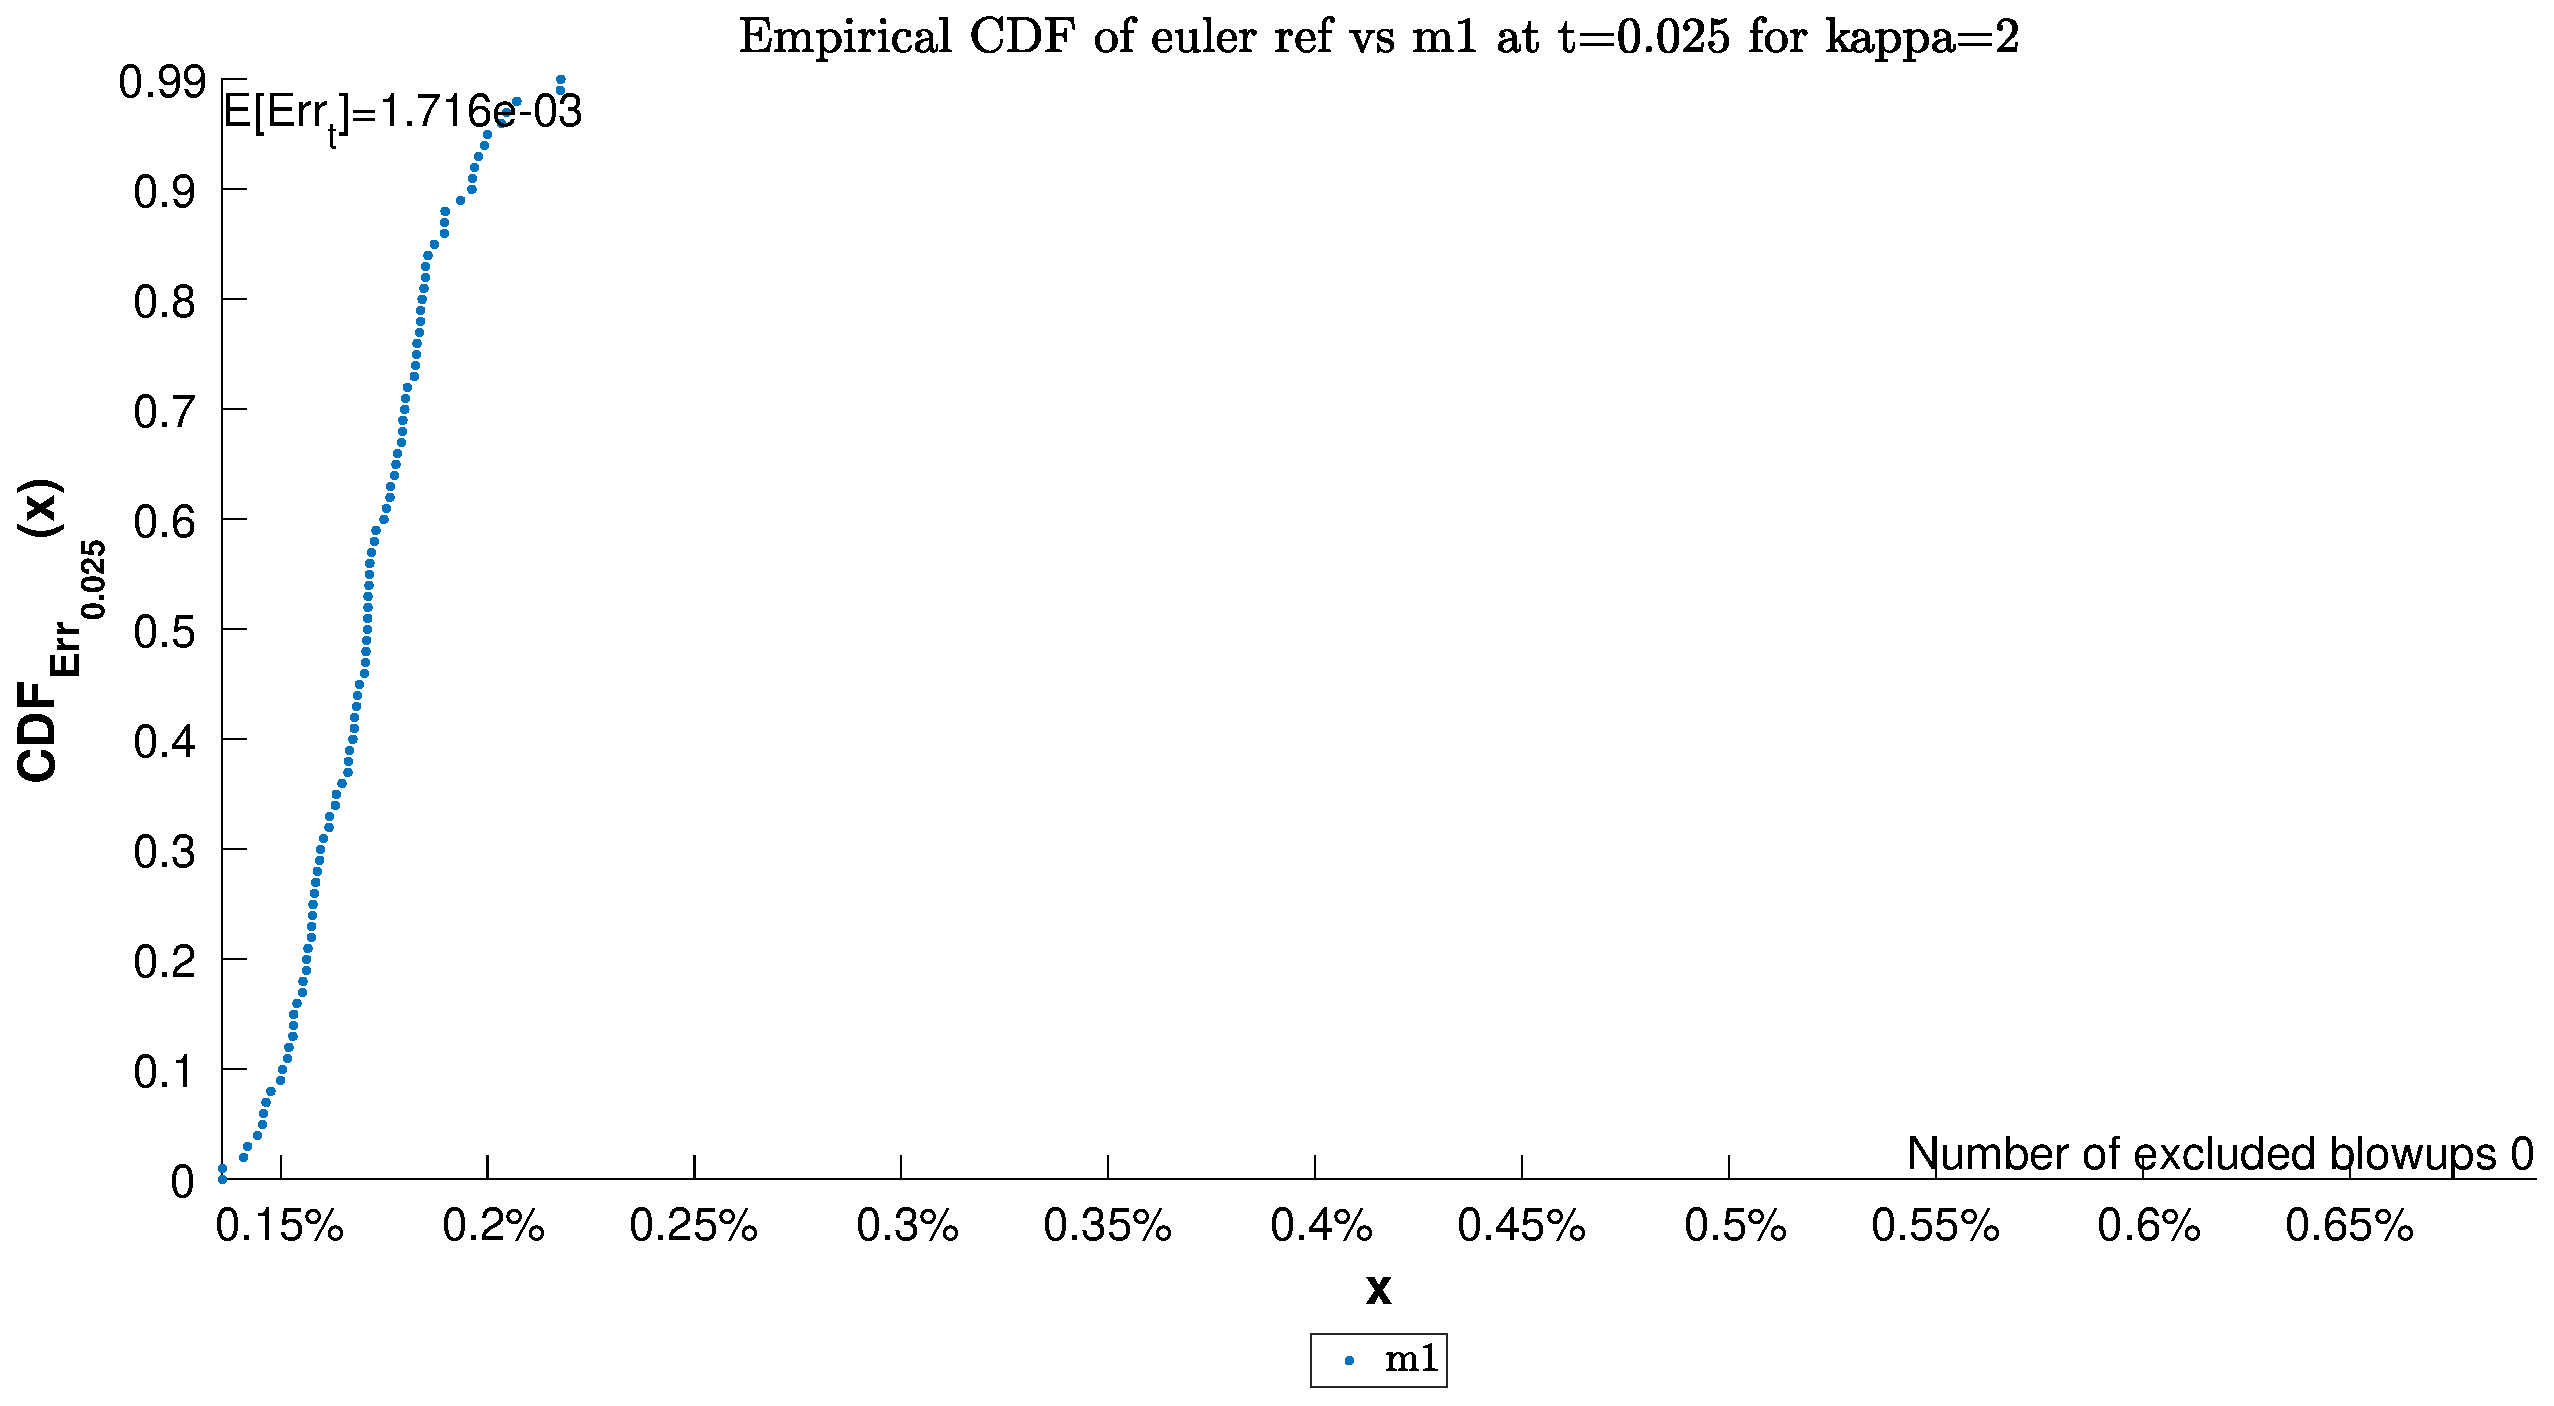
\includegraphics[width=.95\columnwidth]{CDF/CDFEulerRef_11}
\end{landscape}
\begin{landscape}
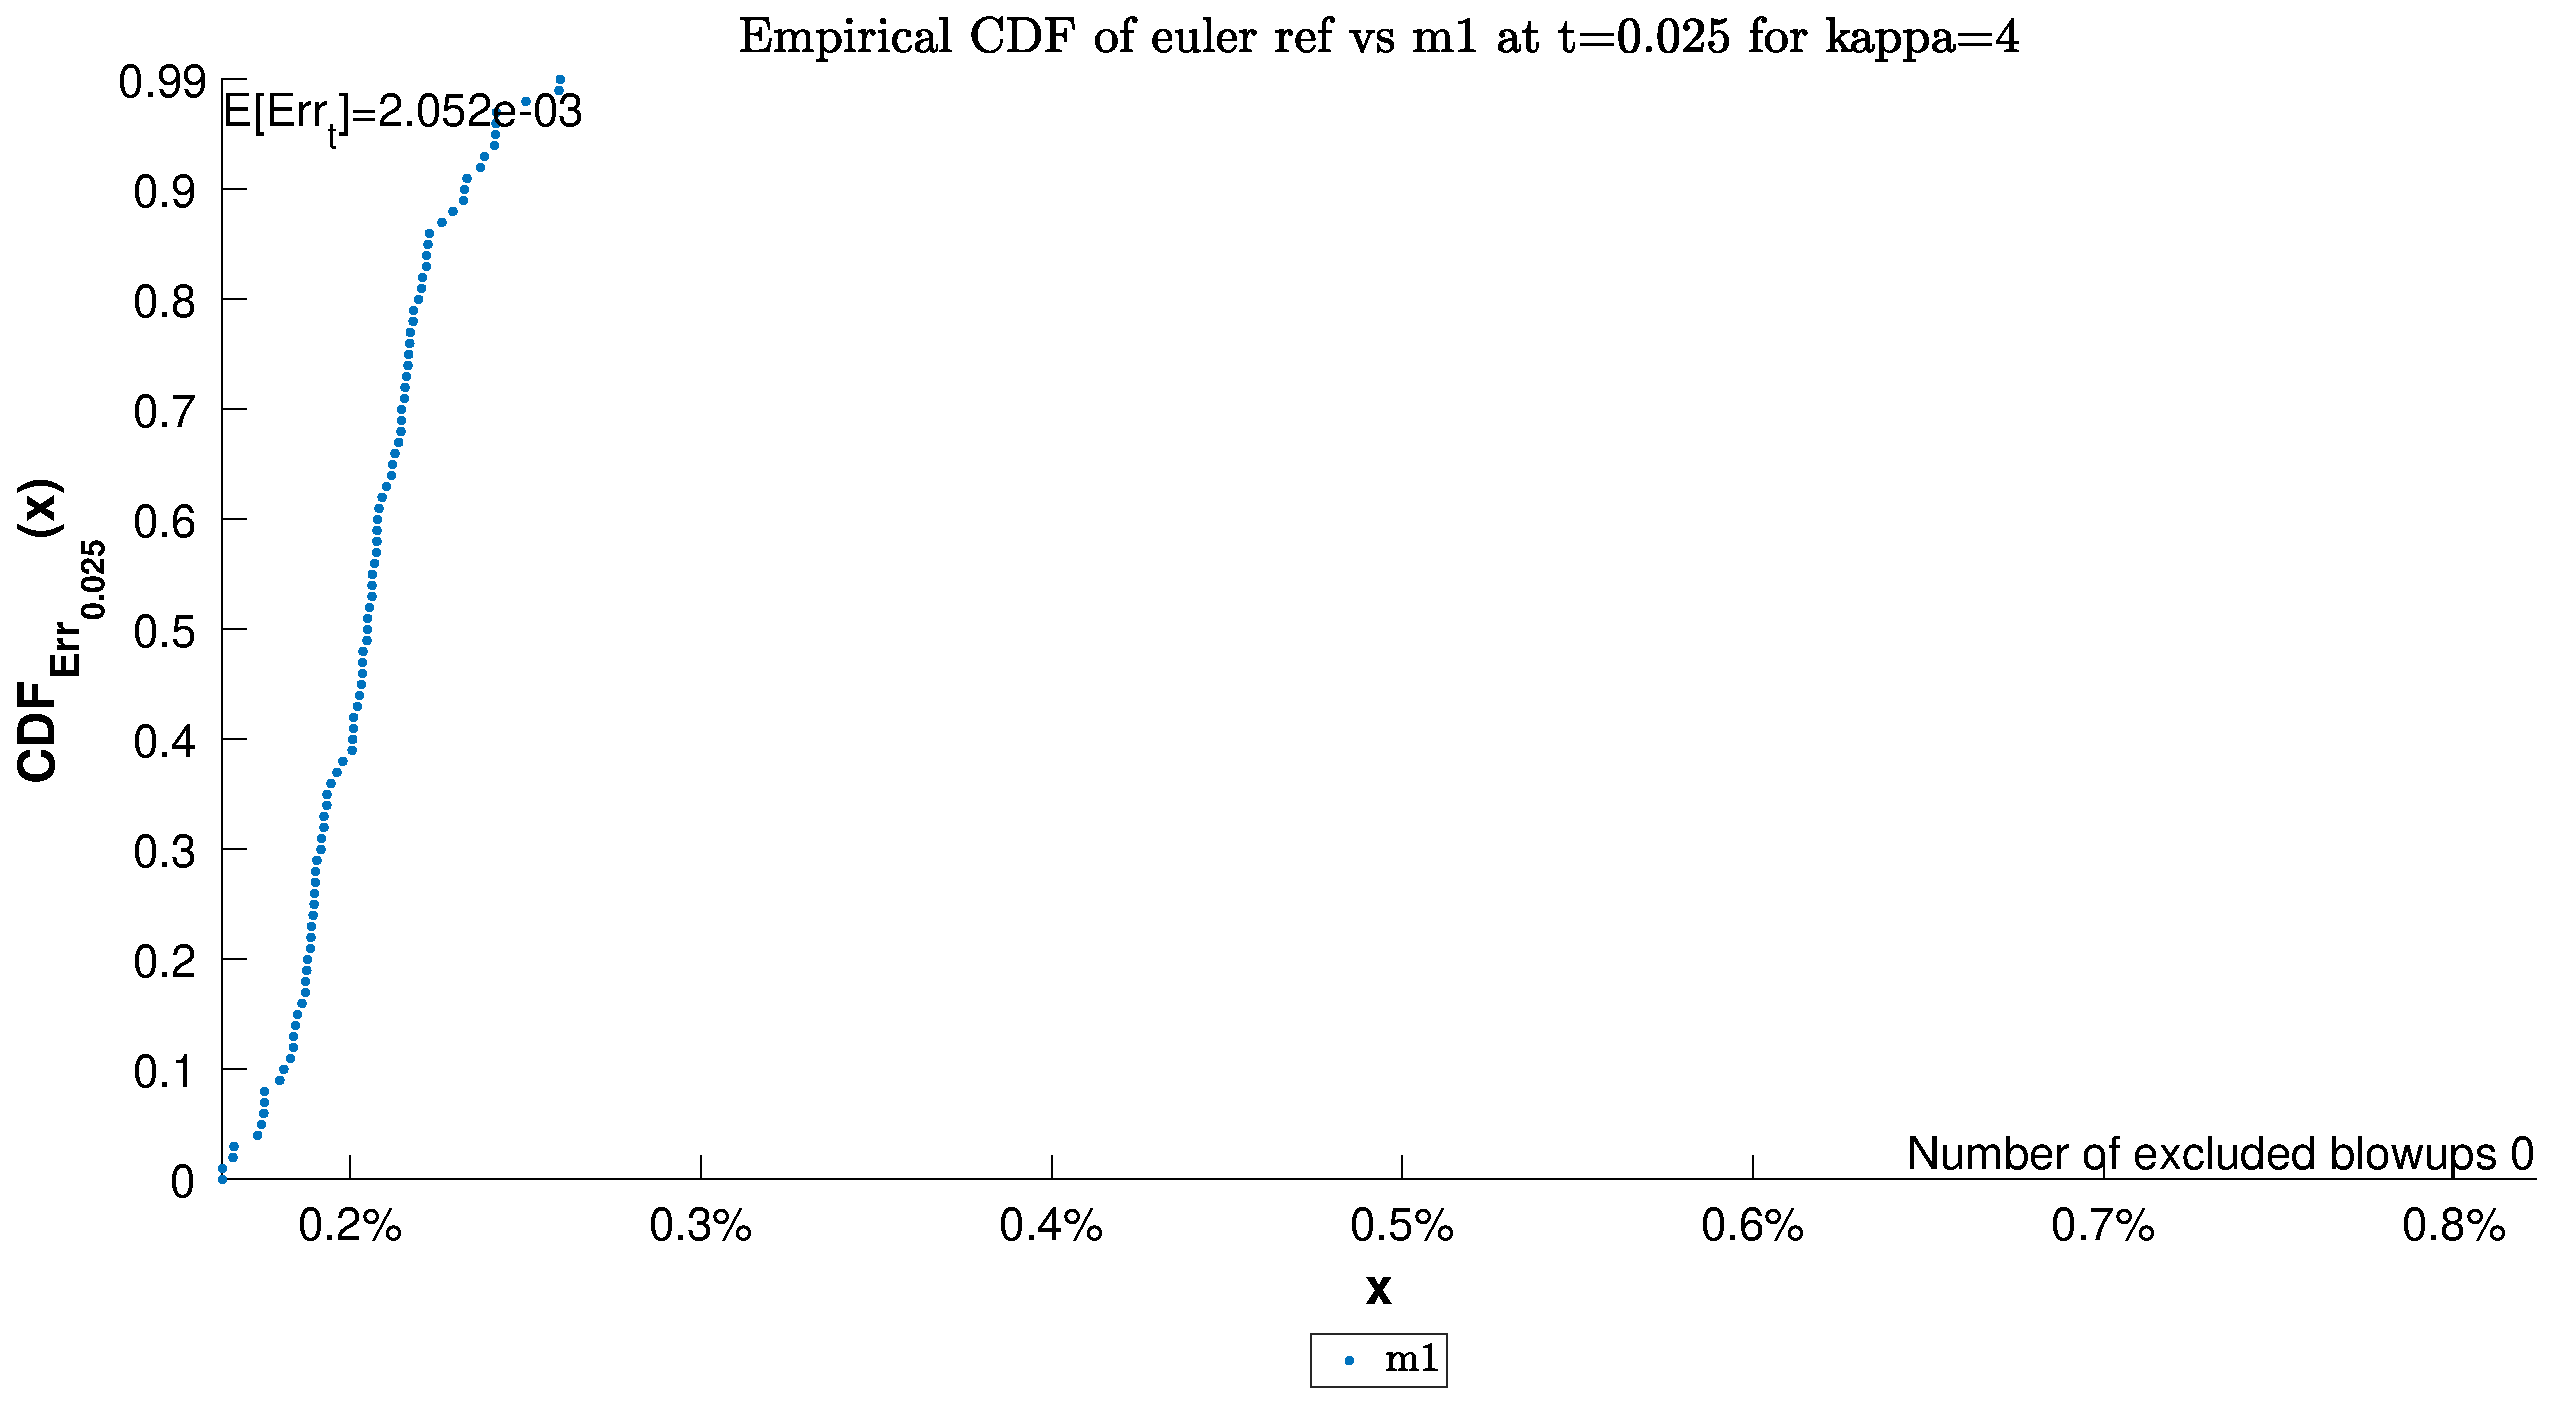
\includegraphics[width=.95\columnwidth]{CDF/CDFEulerRef_12}
\end{landscape}
\begin{landscape}
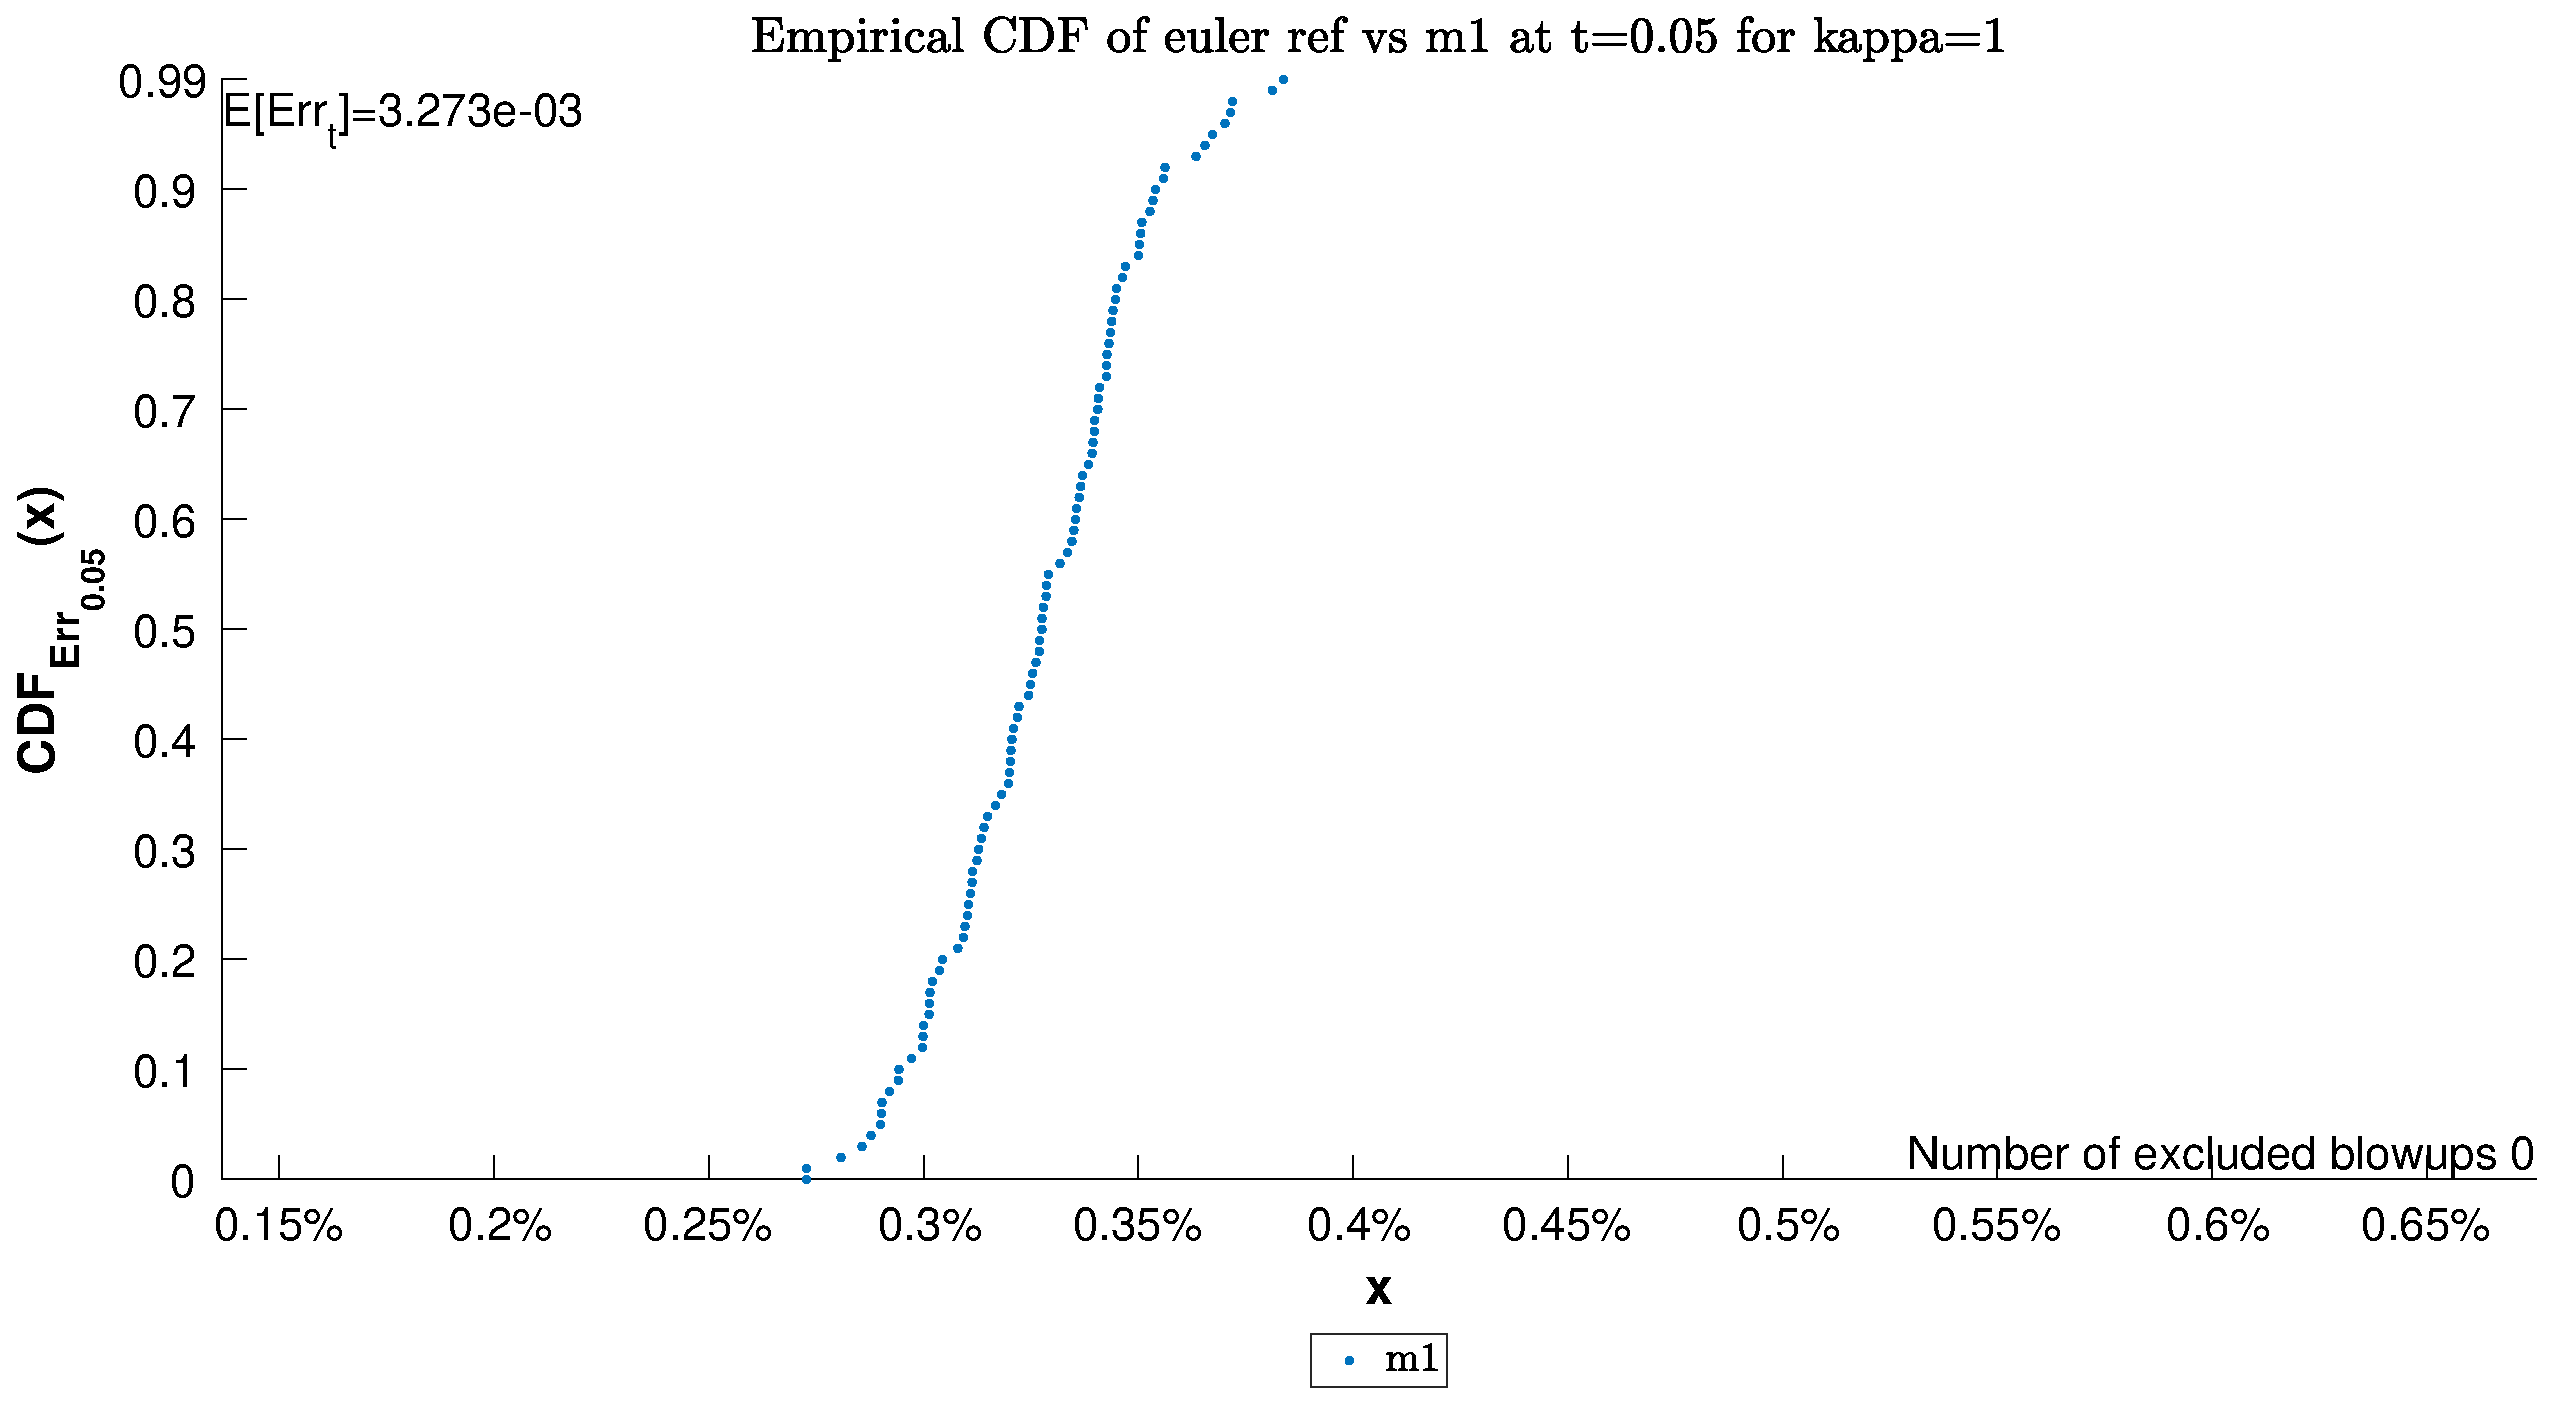
\includegraphics[width=.95\columnwidth]{CDF/CDFEulerRef_13}
\end{landscape}
\begin{landscape}
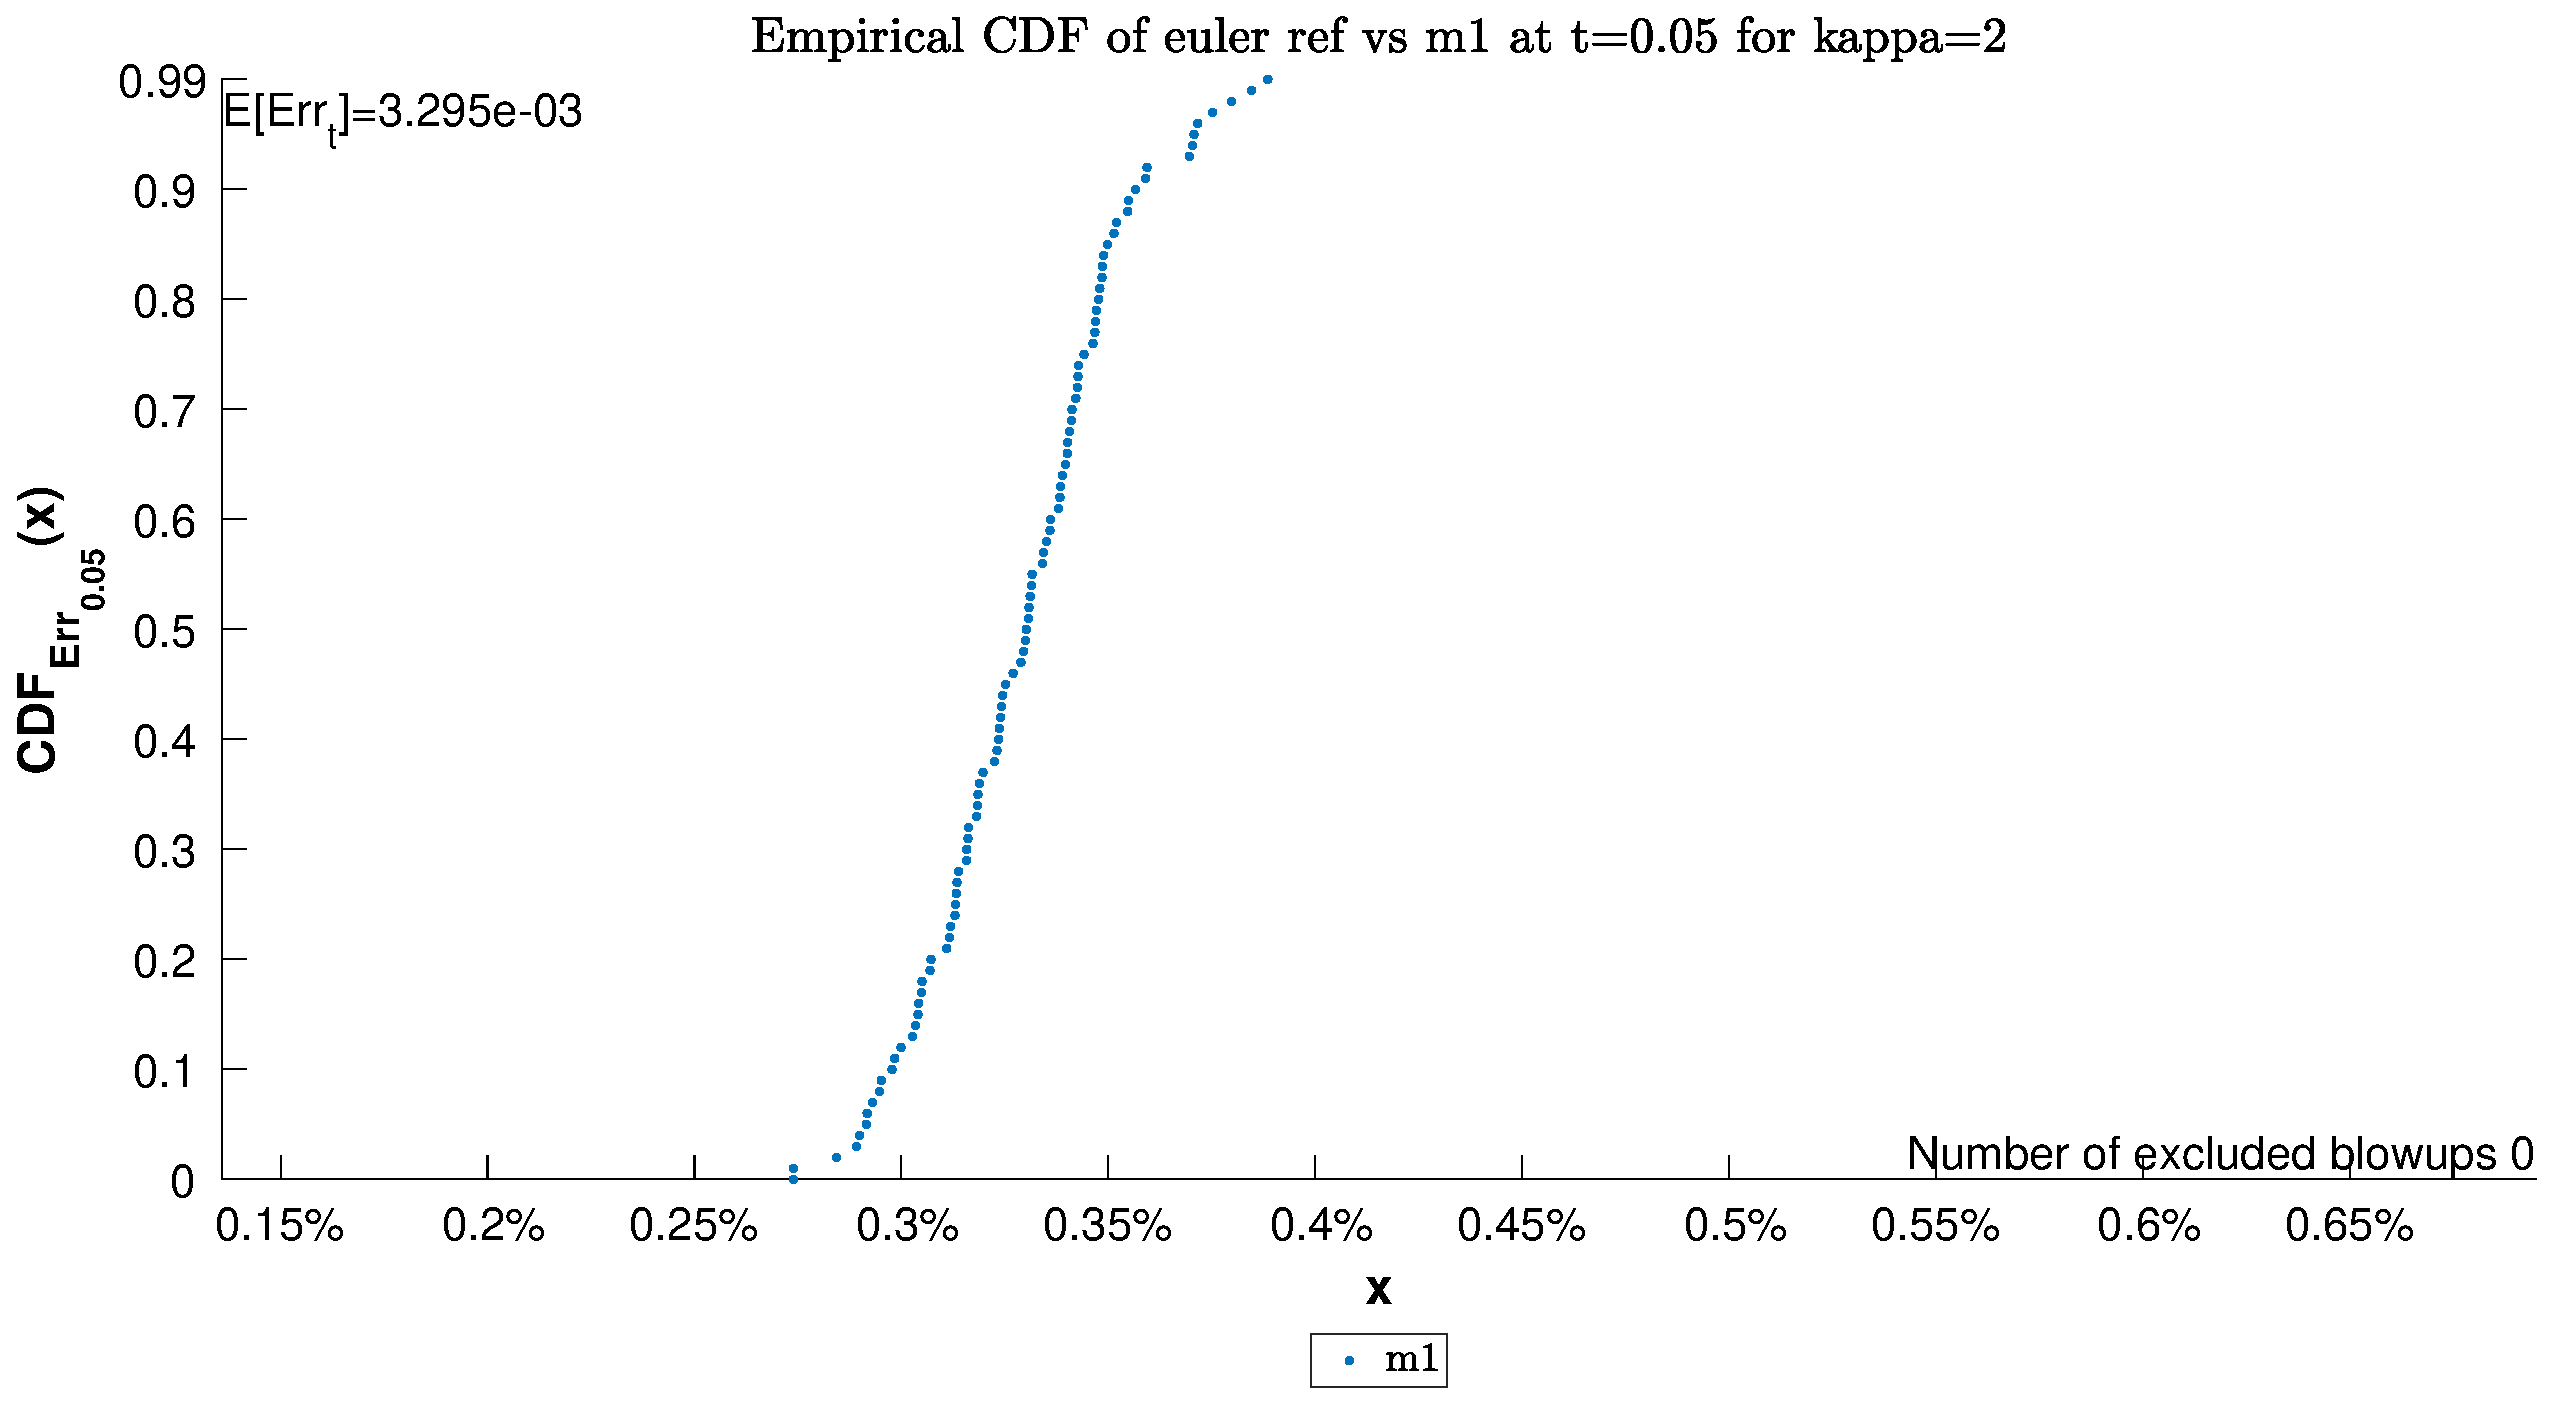
\includegraphics[width=.95\columnwidth]{CDF/CDFEulerRef_14}
\end{landscape}
\begin{landscape}
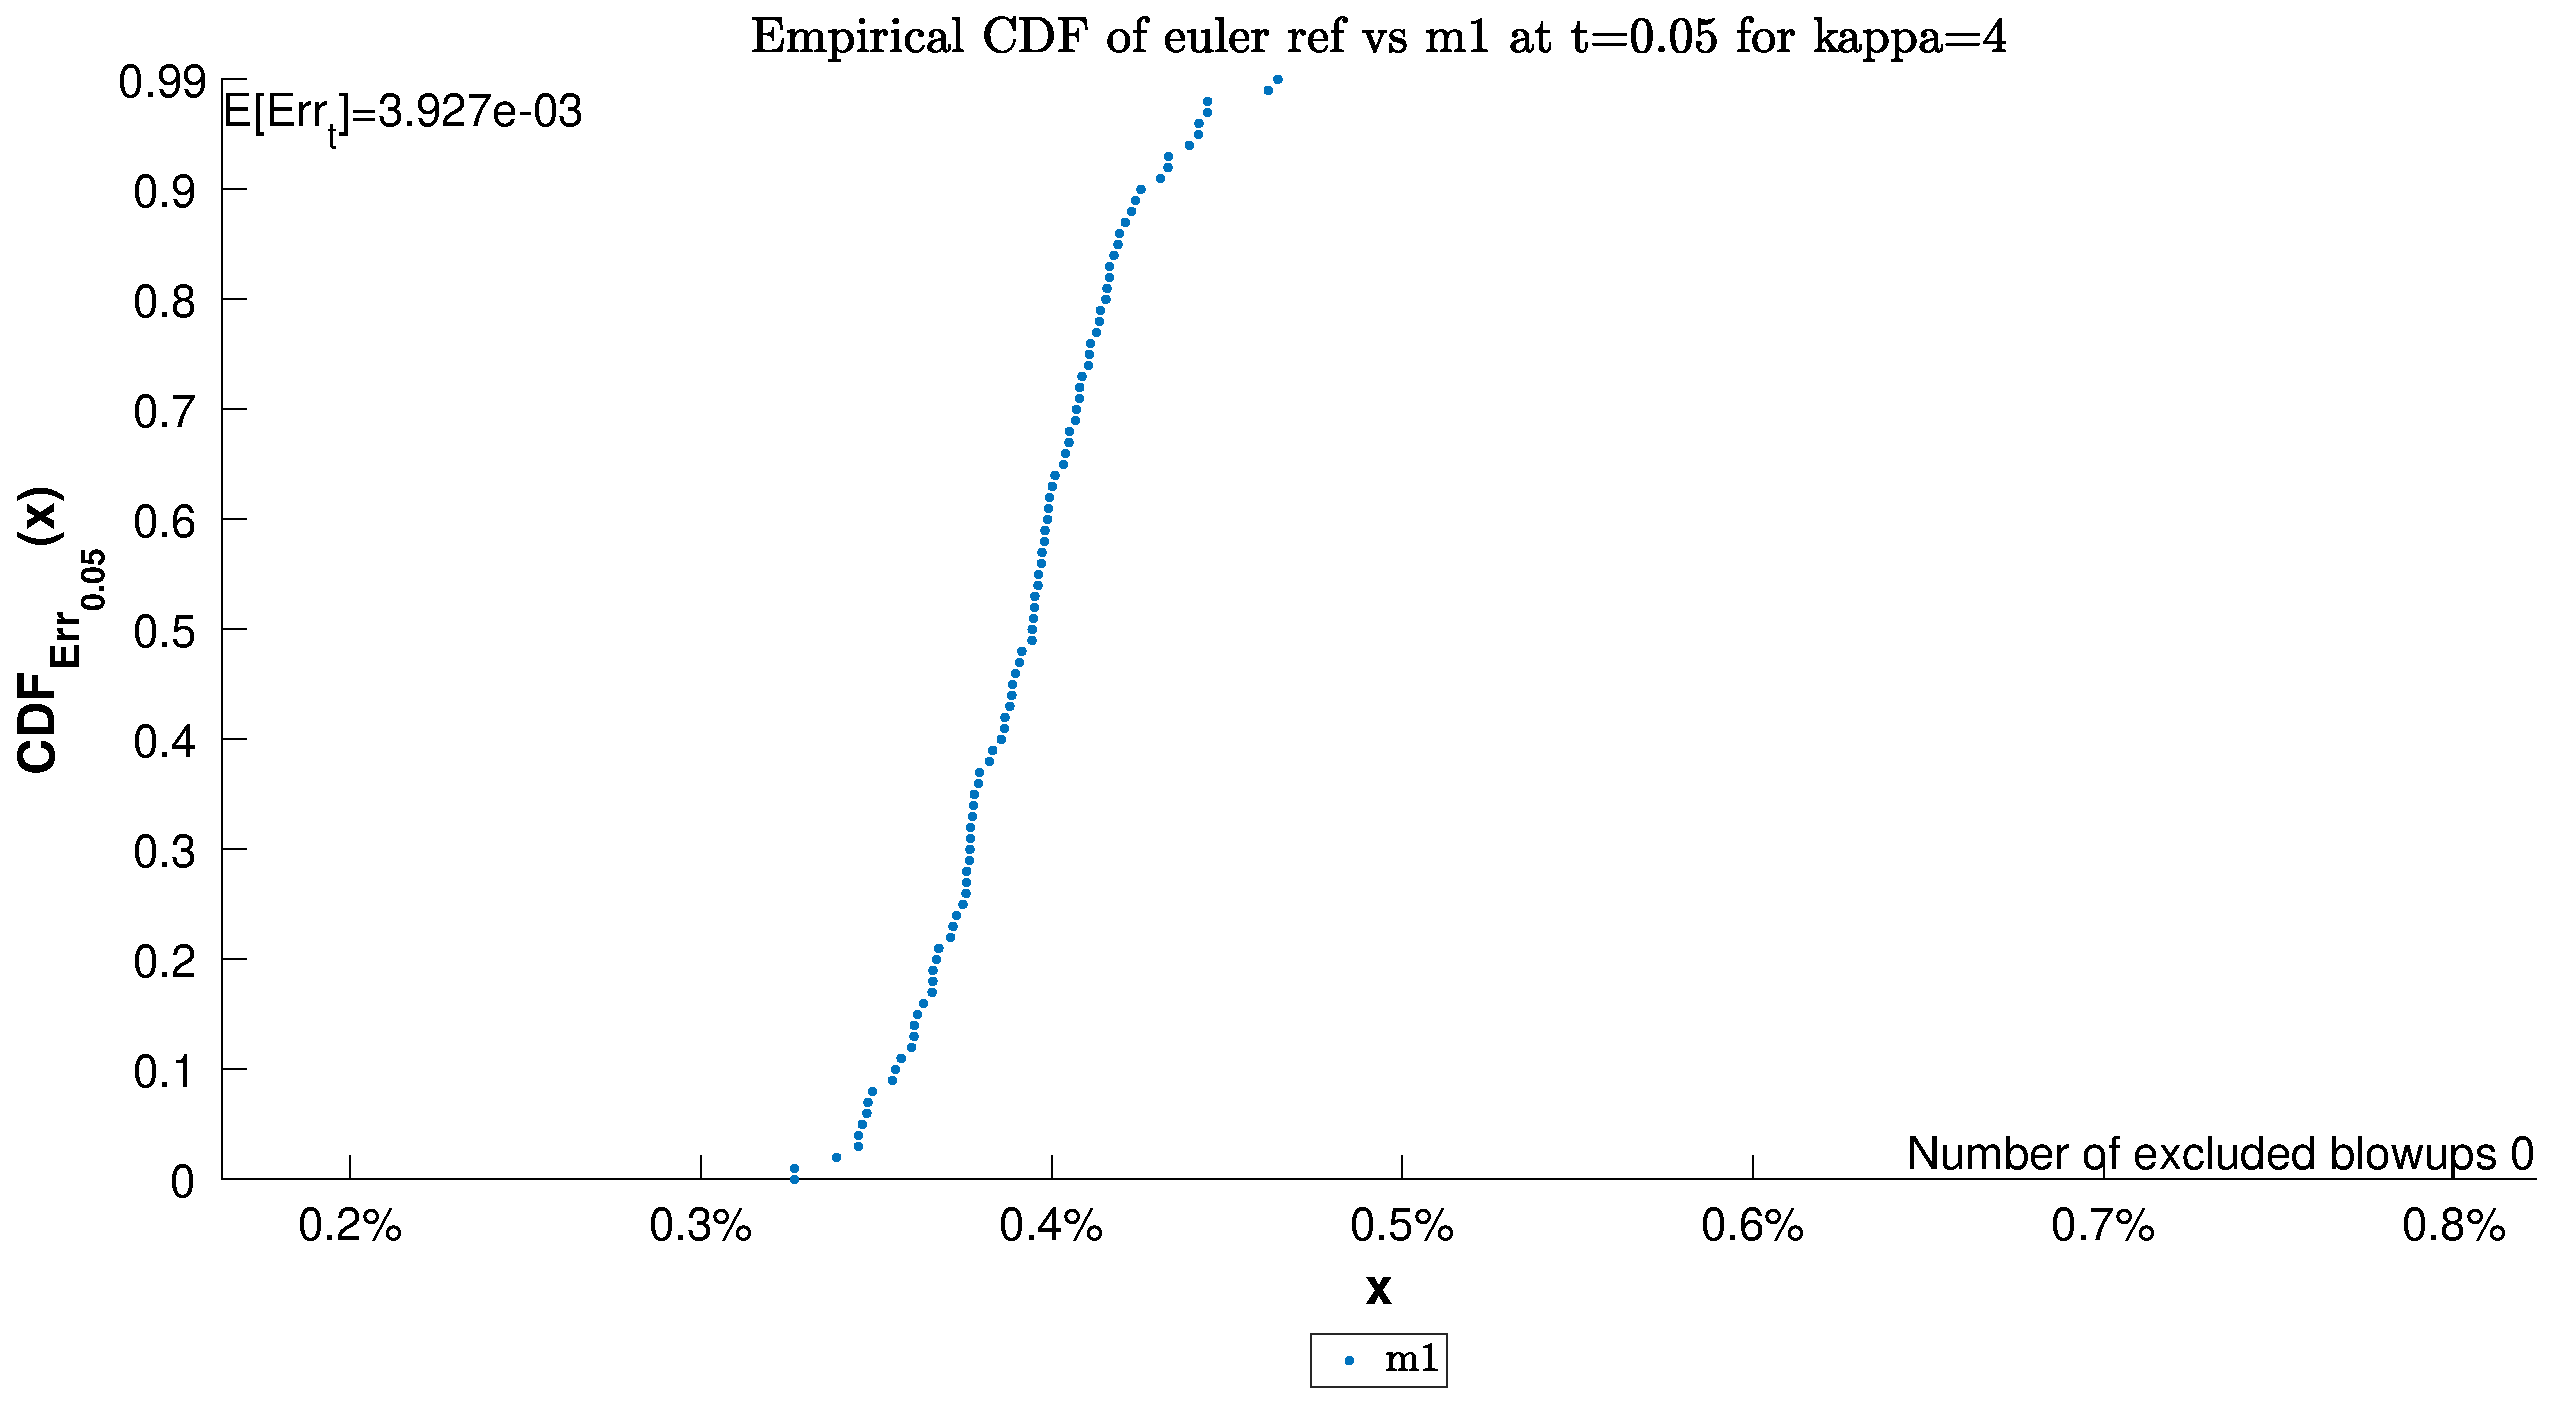
\includegraphics[width=.95\columnwidth]{CDF/CDFEulerRef_15}
\end{landscape}
\begin{landscape}
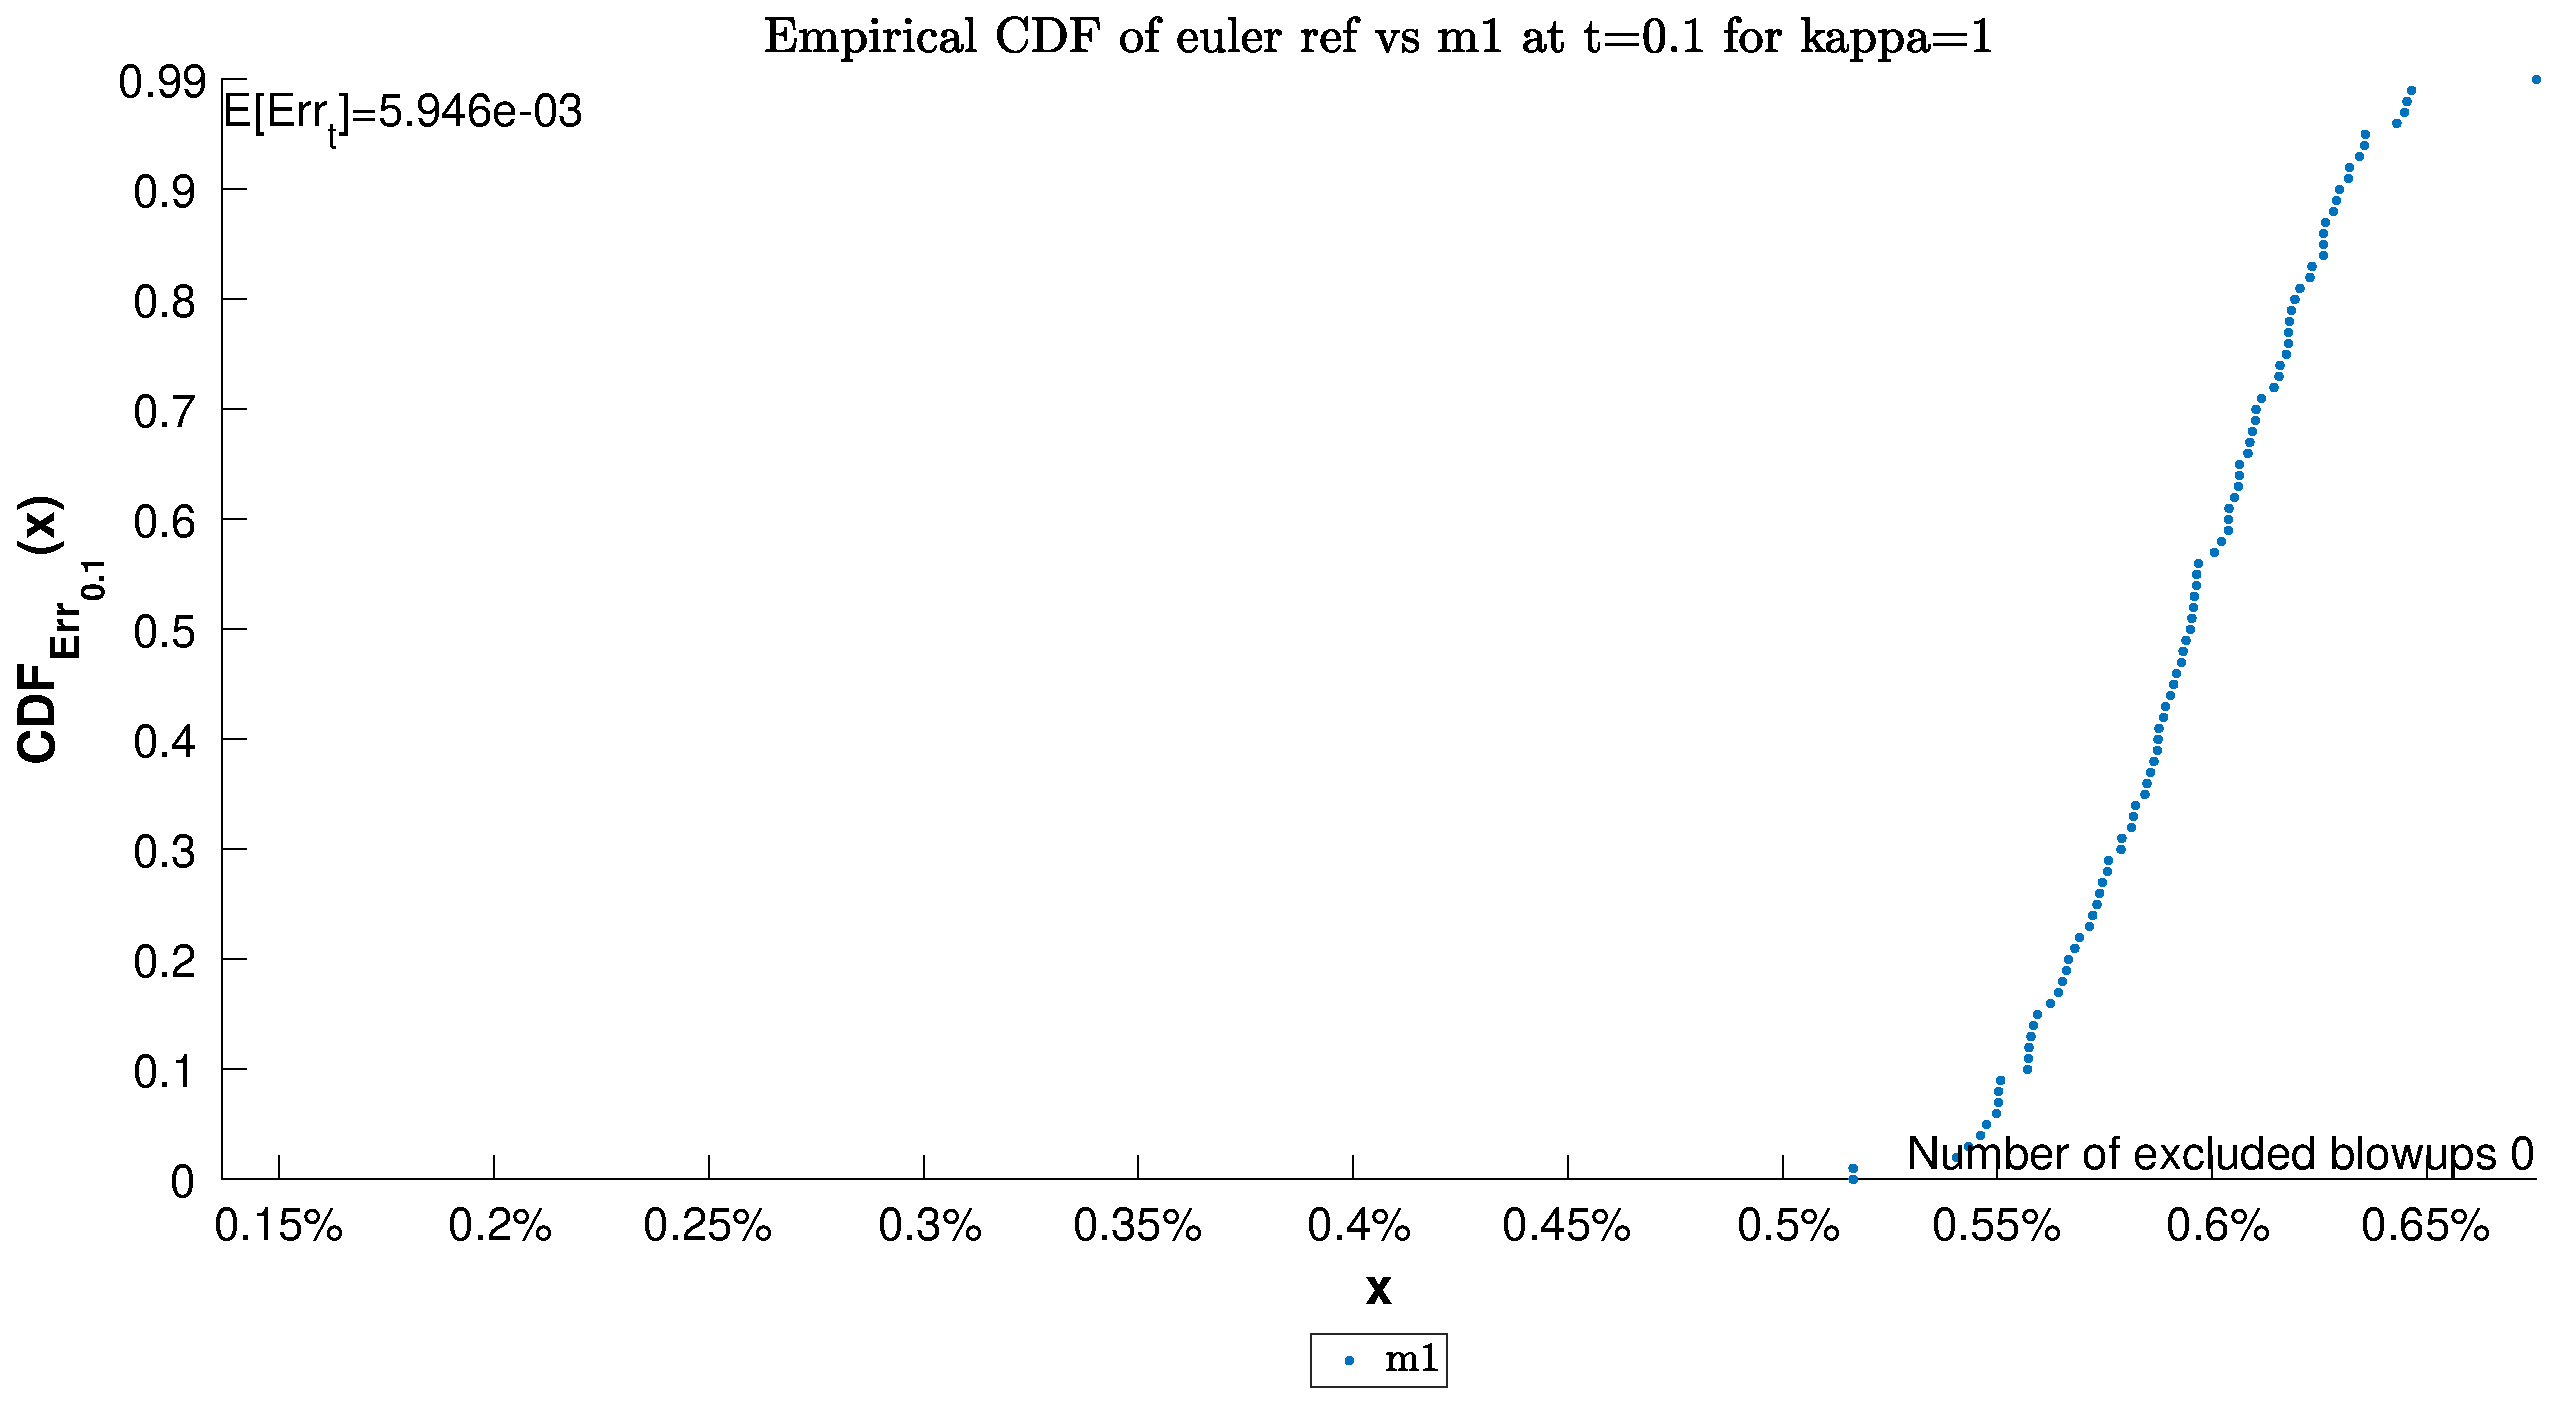
\includegraphics[width=.95\columnwidth]{CDF/CDFEulerRef_16}
\end{landscape}
\begin{landscape}
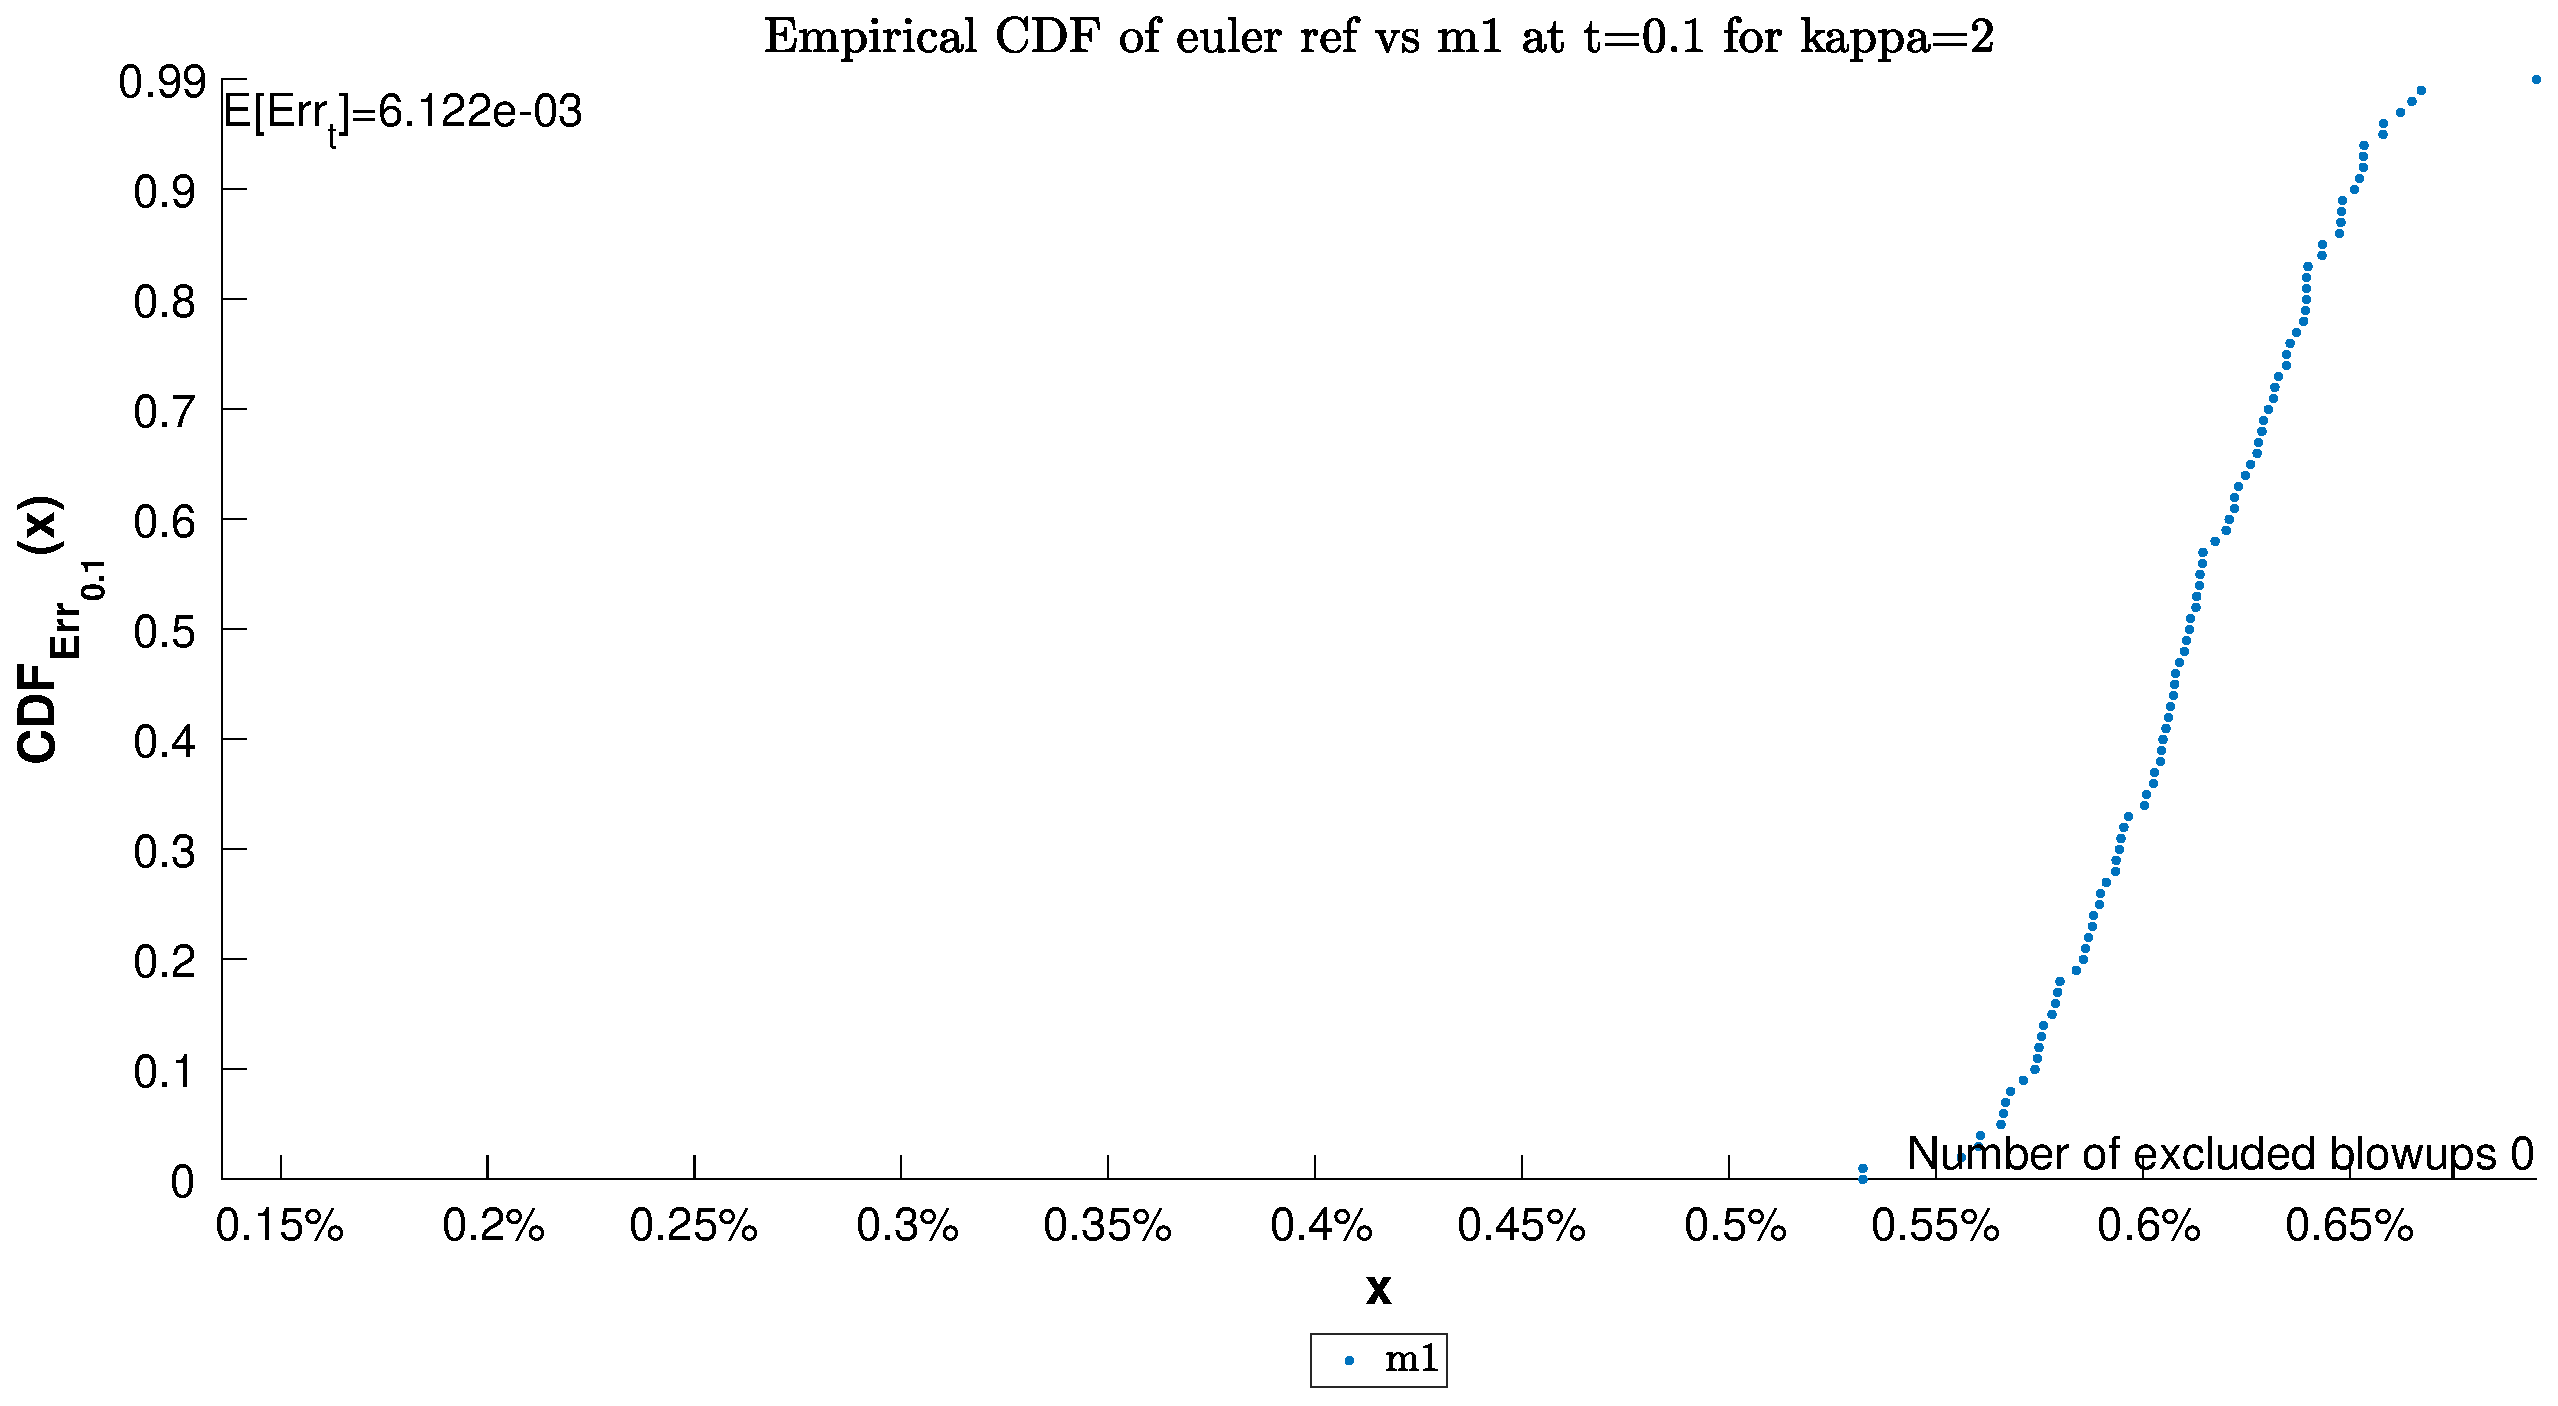
\includegraphics[width=.95\columnwidth]{CDF/CDFEulerRef_17}
\end{landscape}
\begin{landscape}
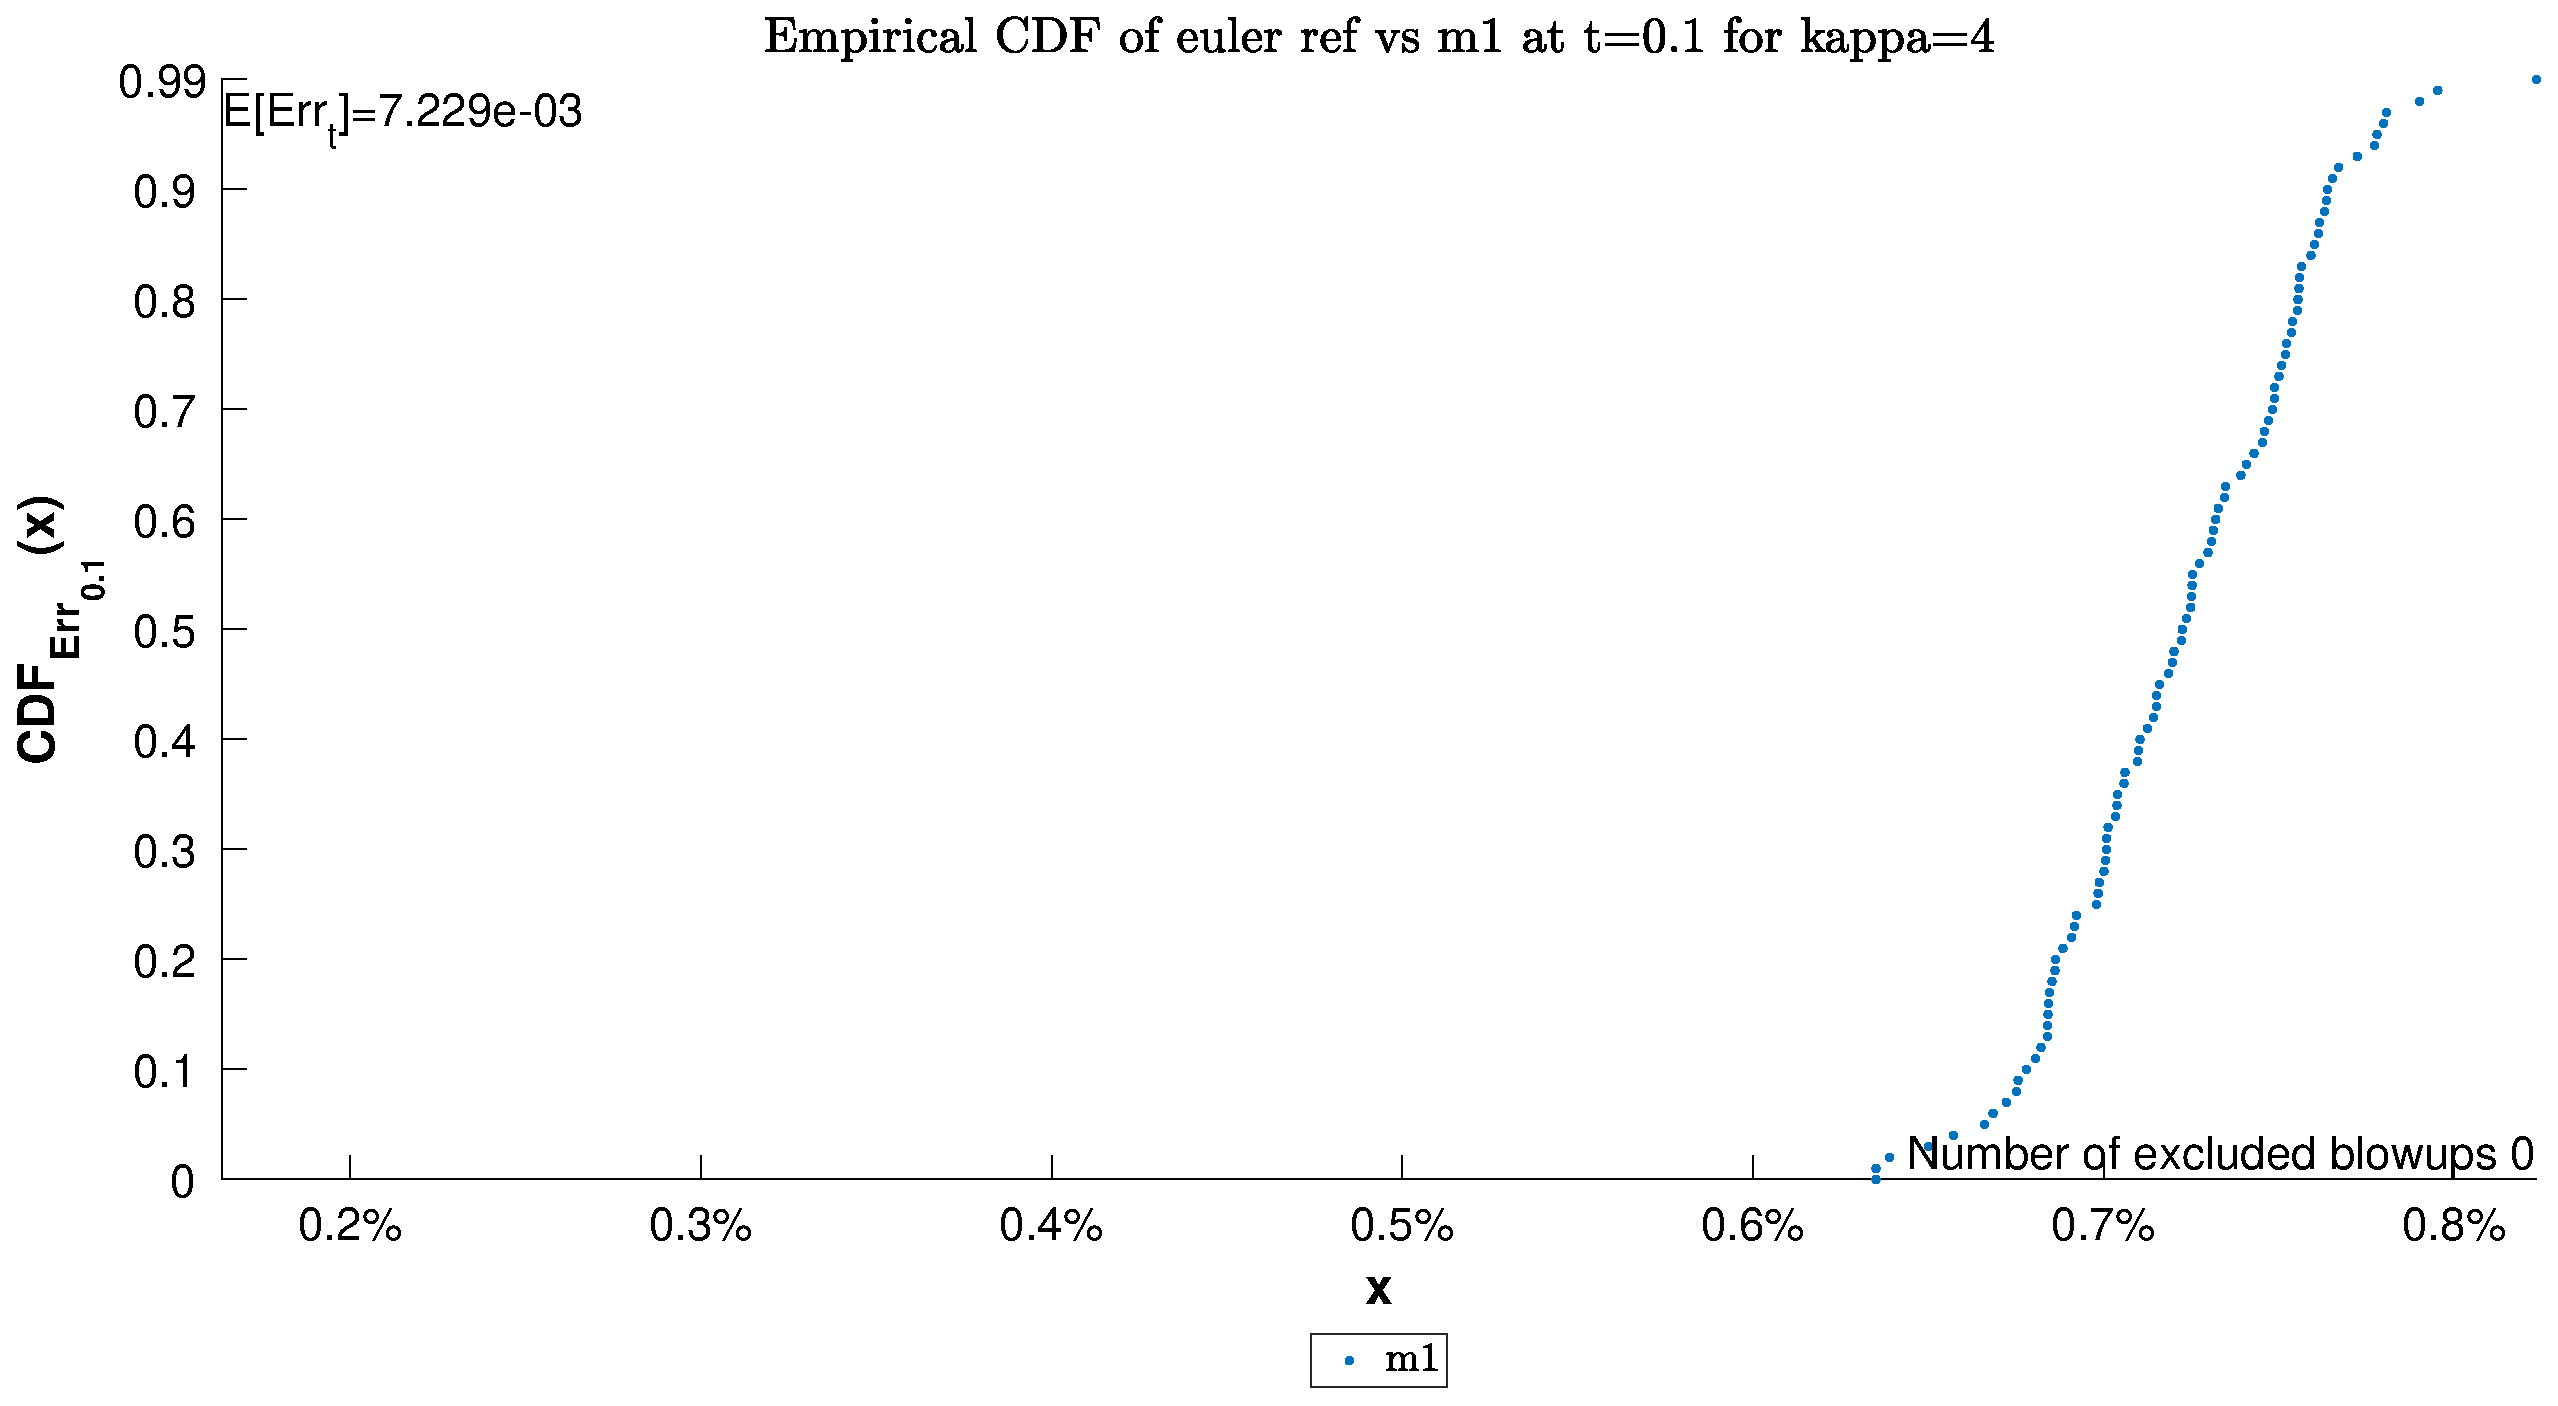
\includegraphics[width=.95\columnwidth]{CDF/CDFEulerRef_18}
\end{landscape}
\begin{landscape}
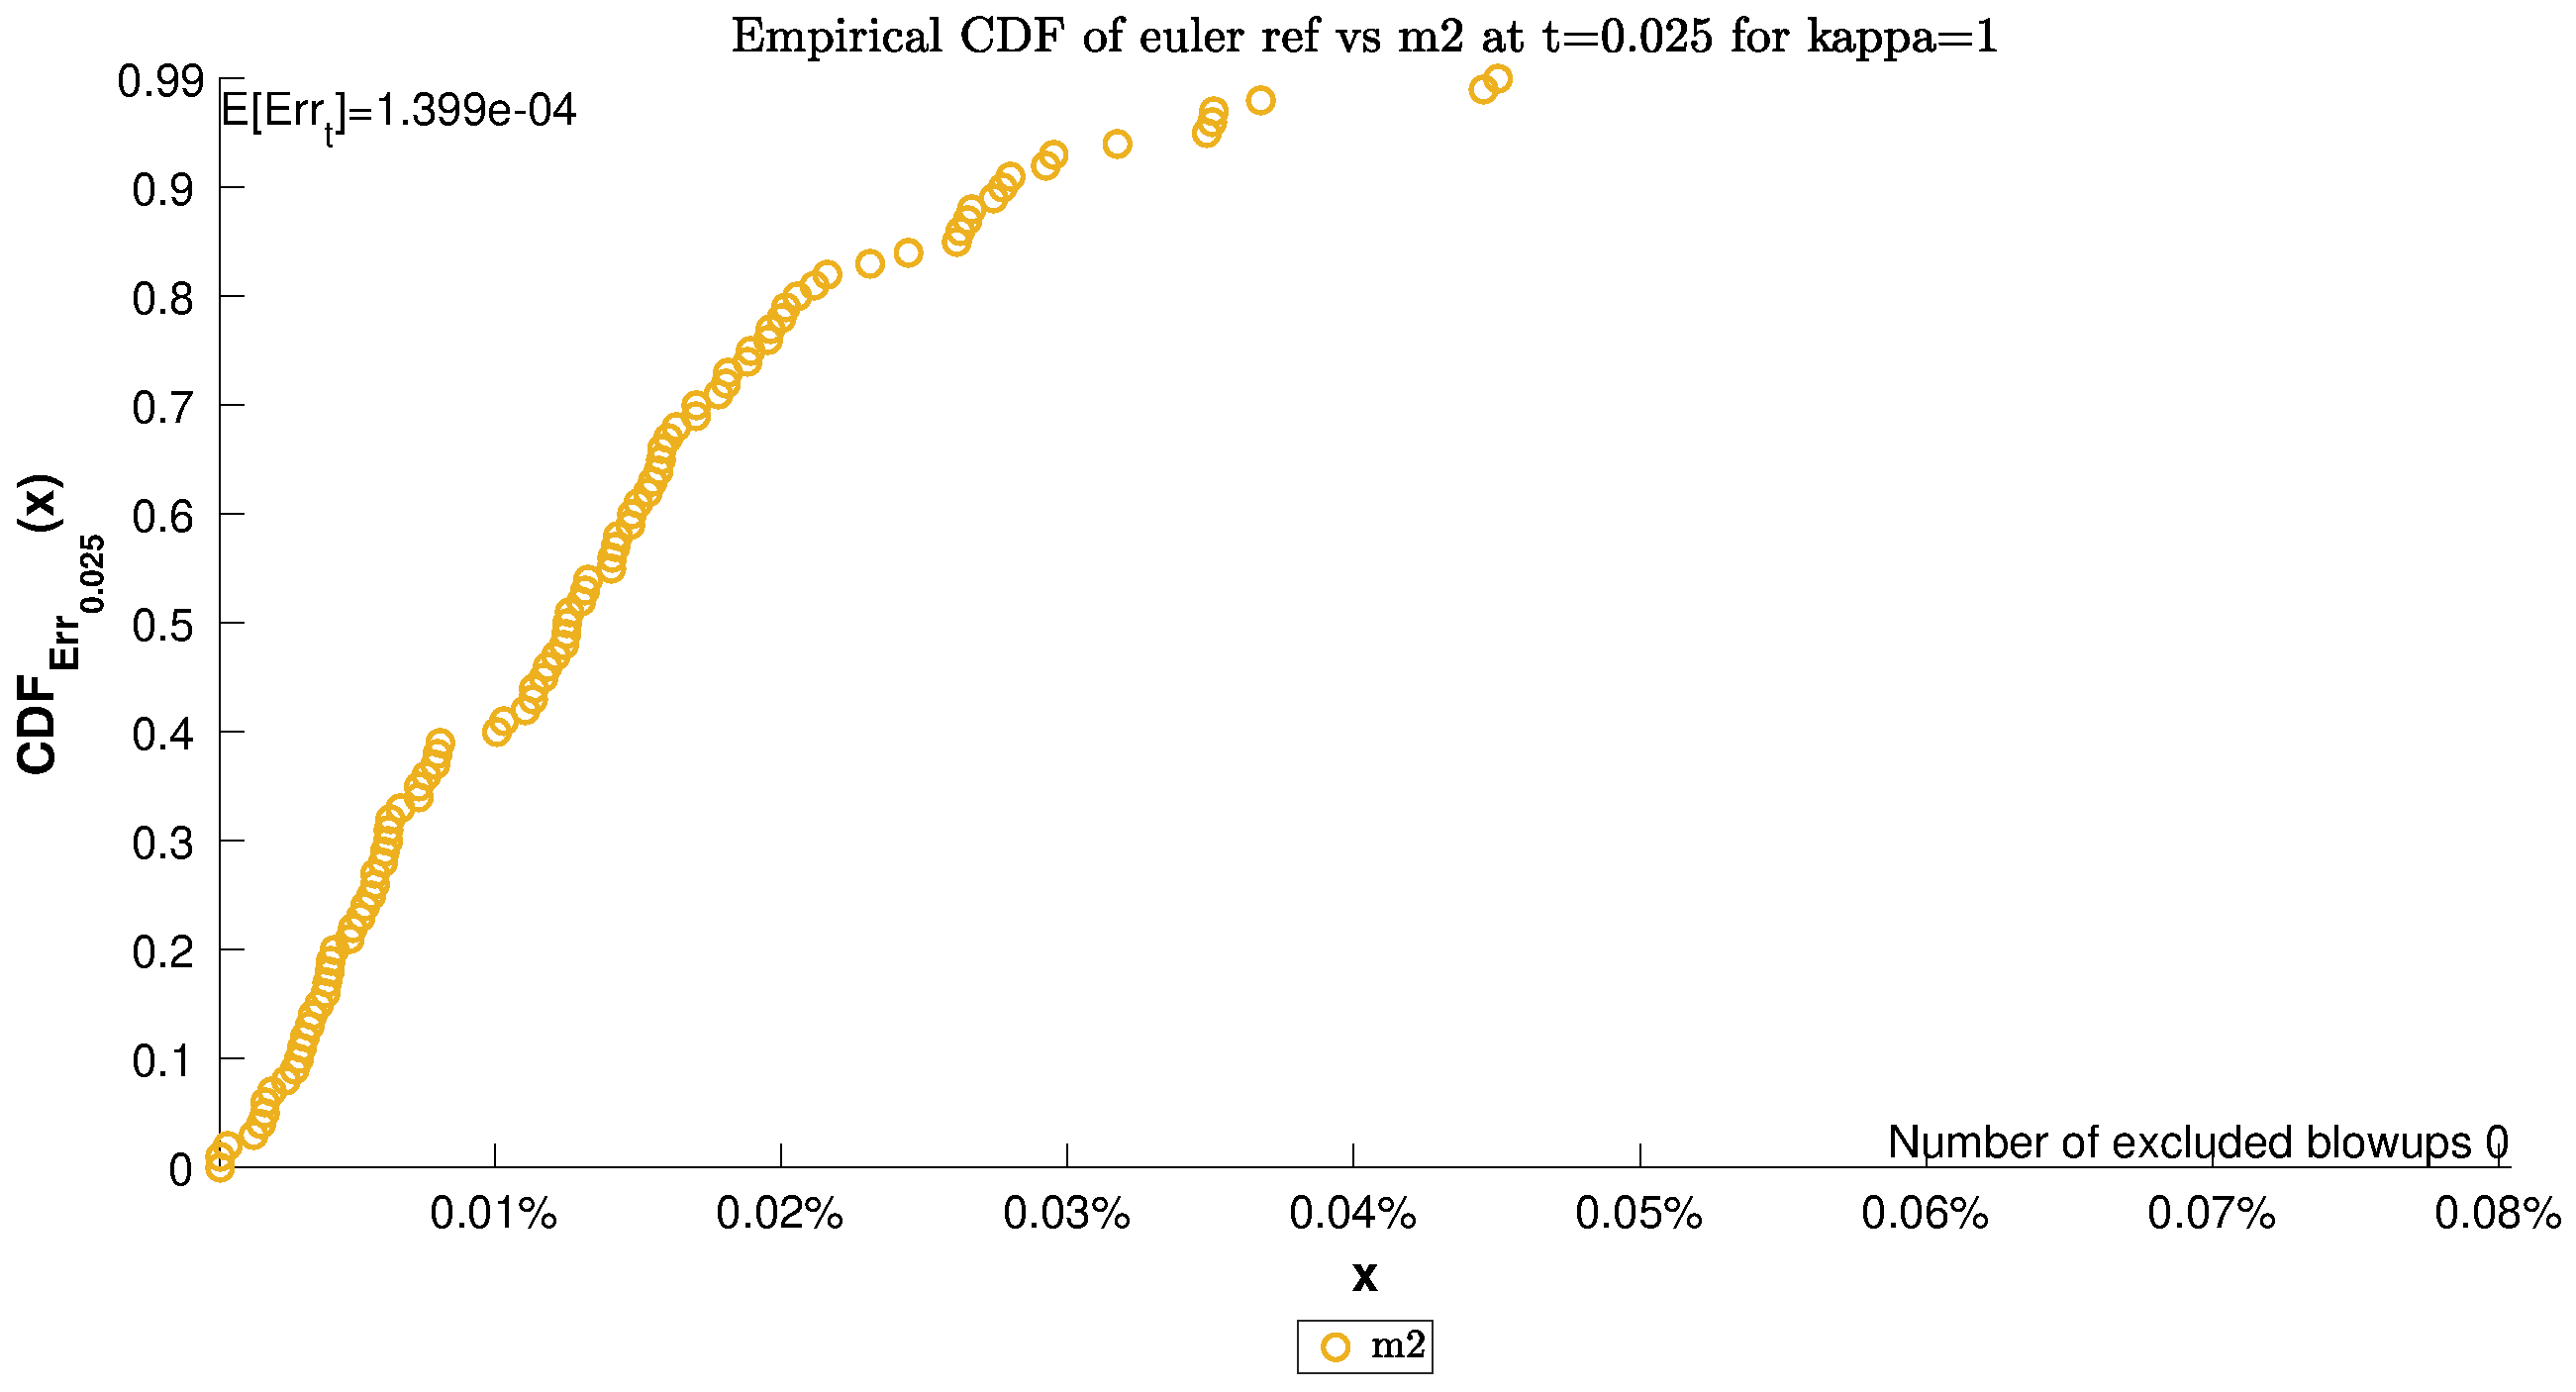
\includegraphics[width=.95\columnwidth]{CDF/CDFEulerRef_19}
\end{landscape}
\begin{landscape}
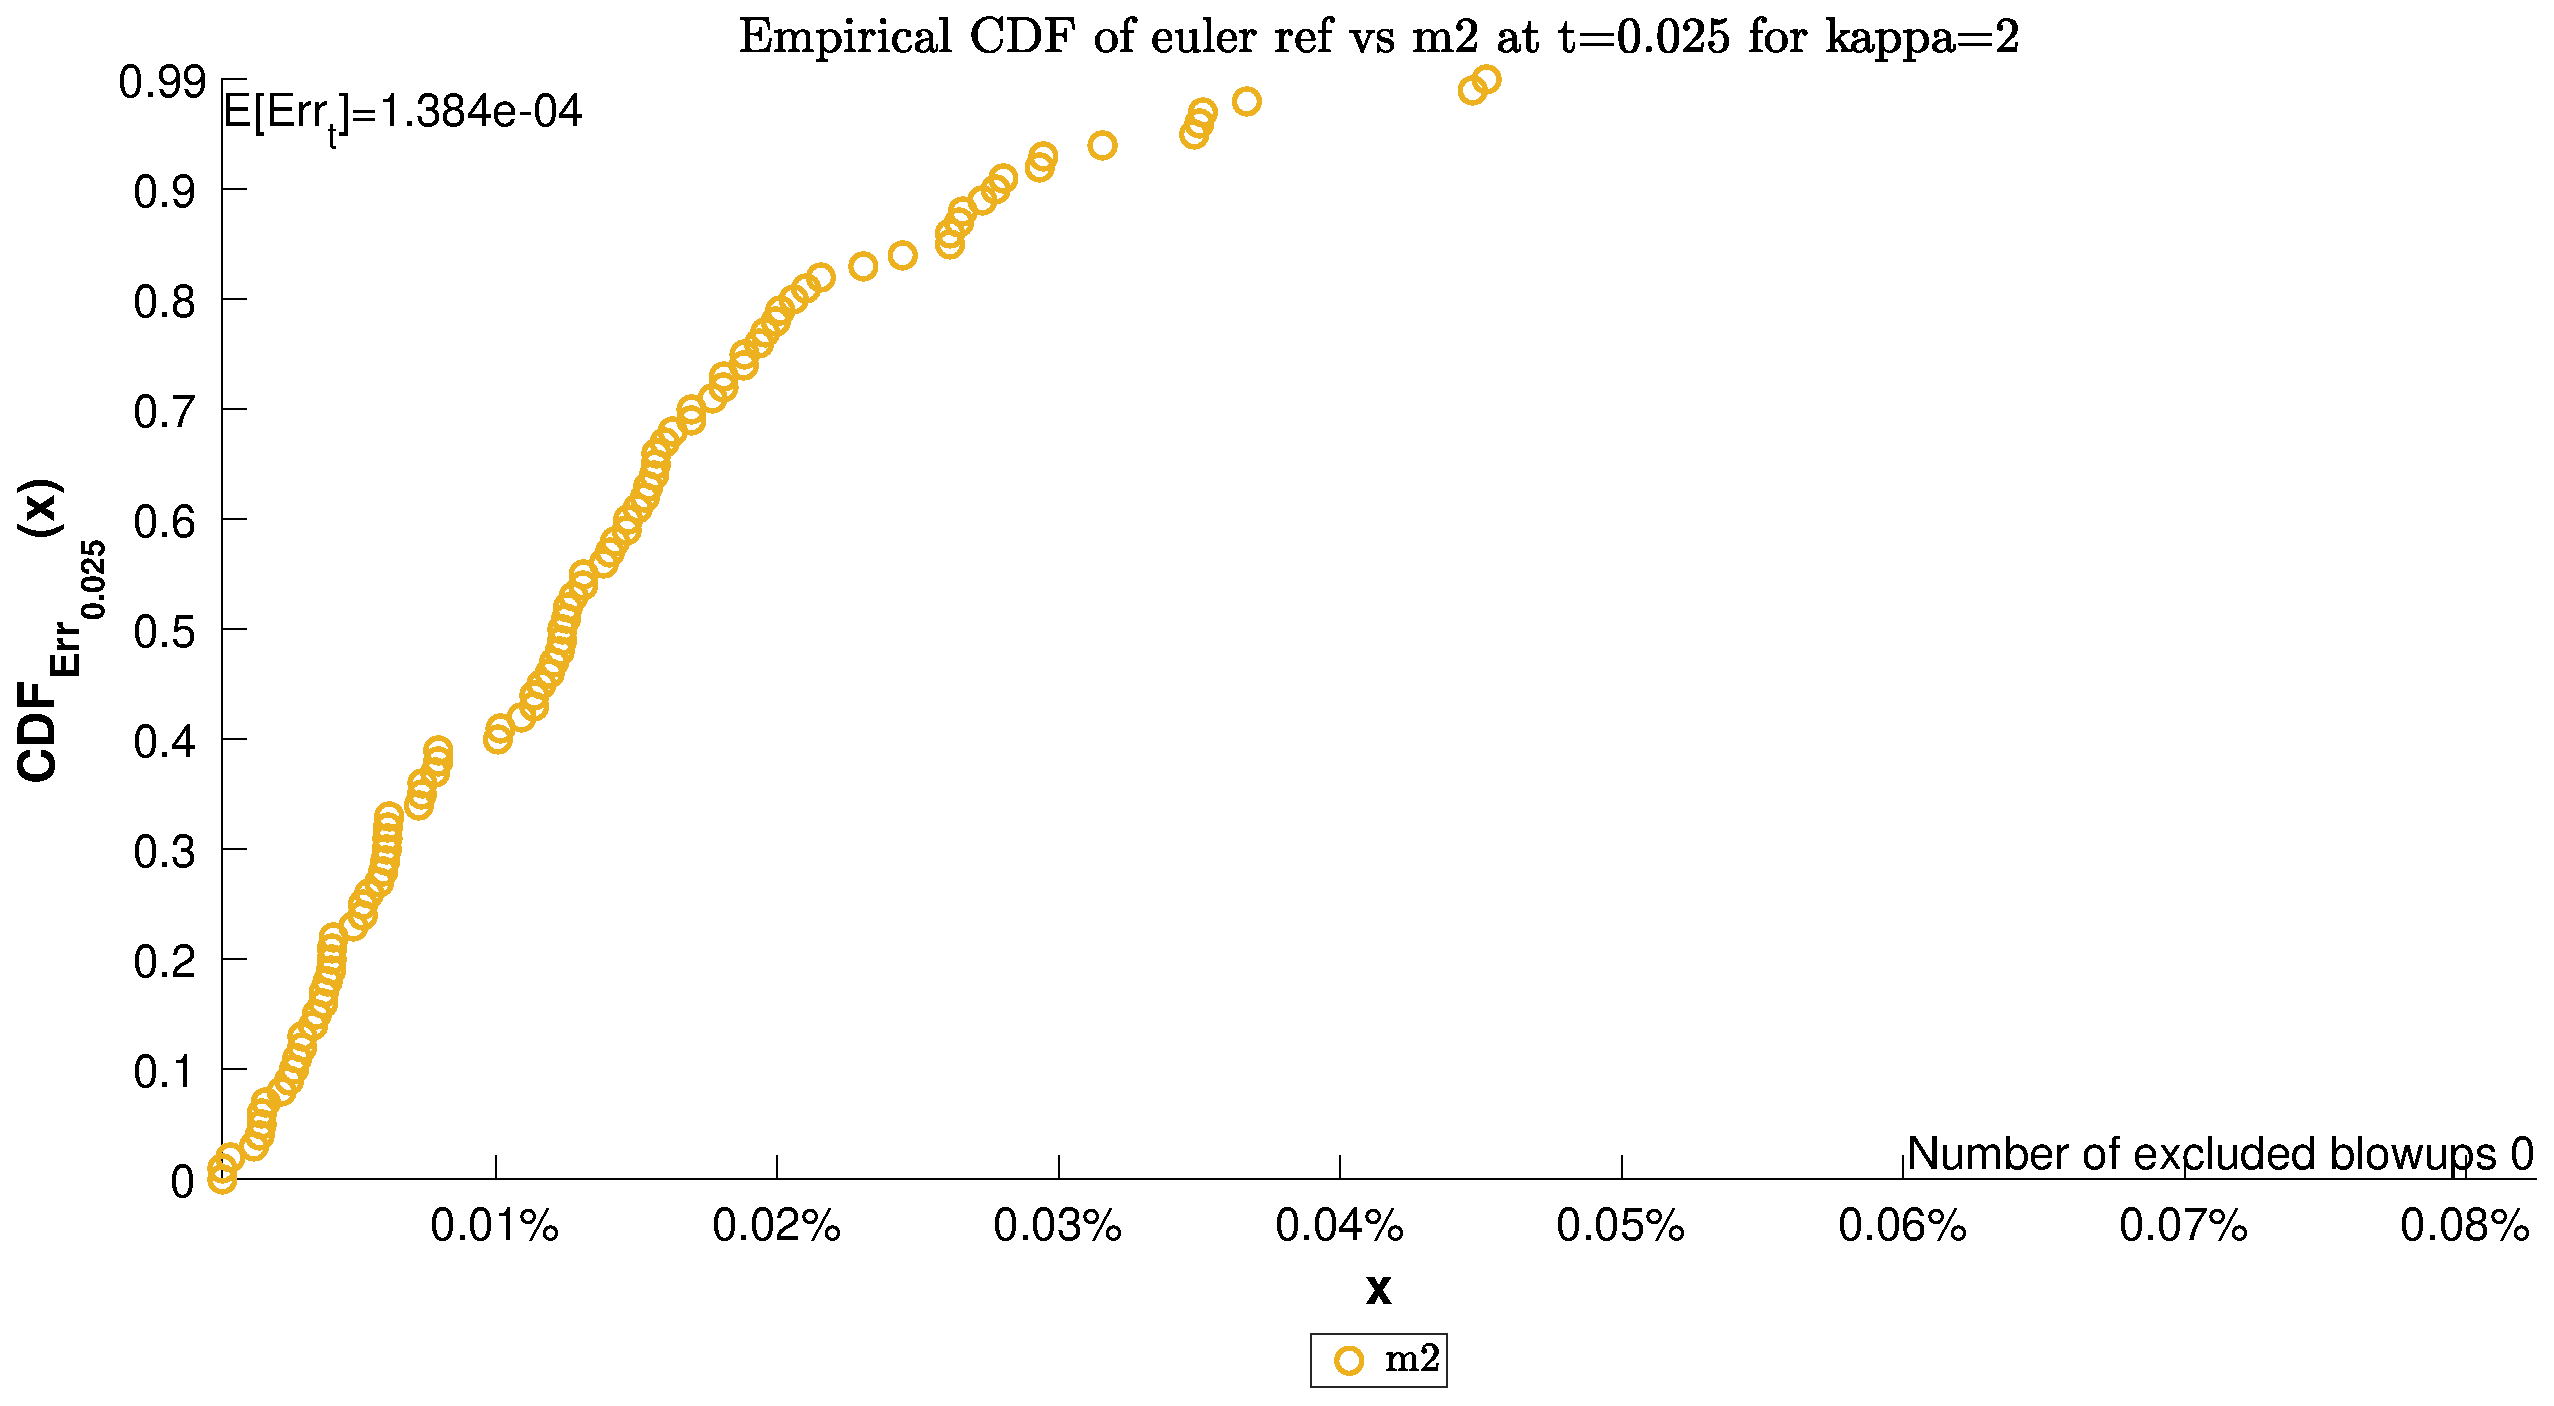
\includegraphics[width=.95\columnwidth]{CDF/CDFEulerRef_20}
\end{landscape}
\begin{landscape}
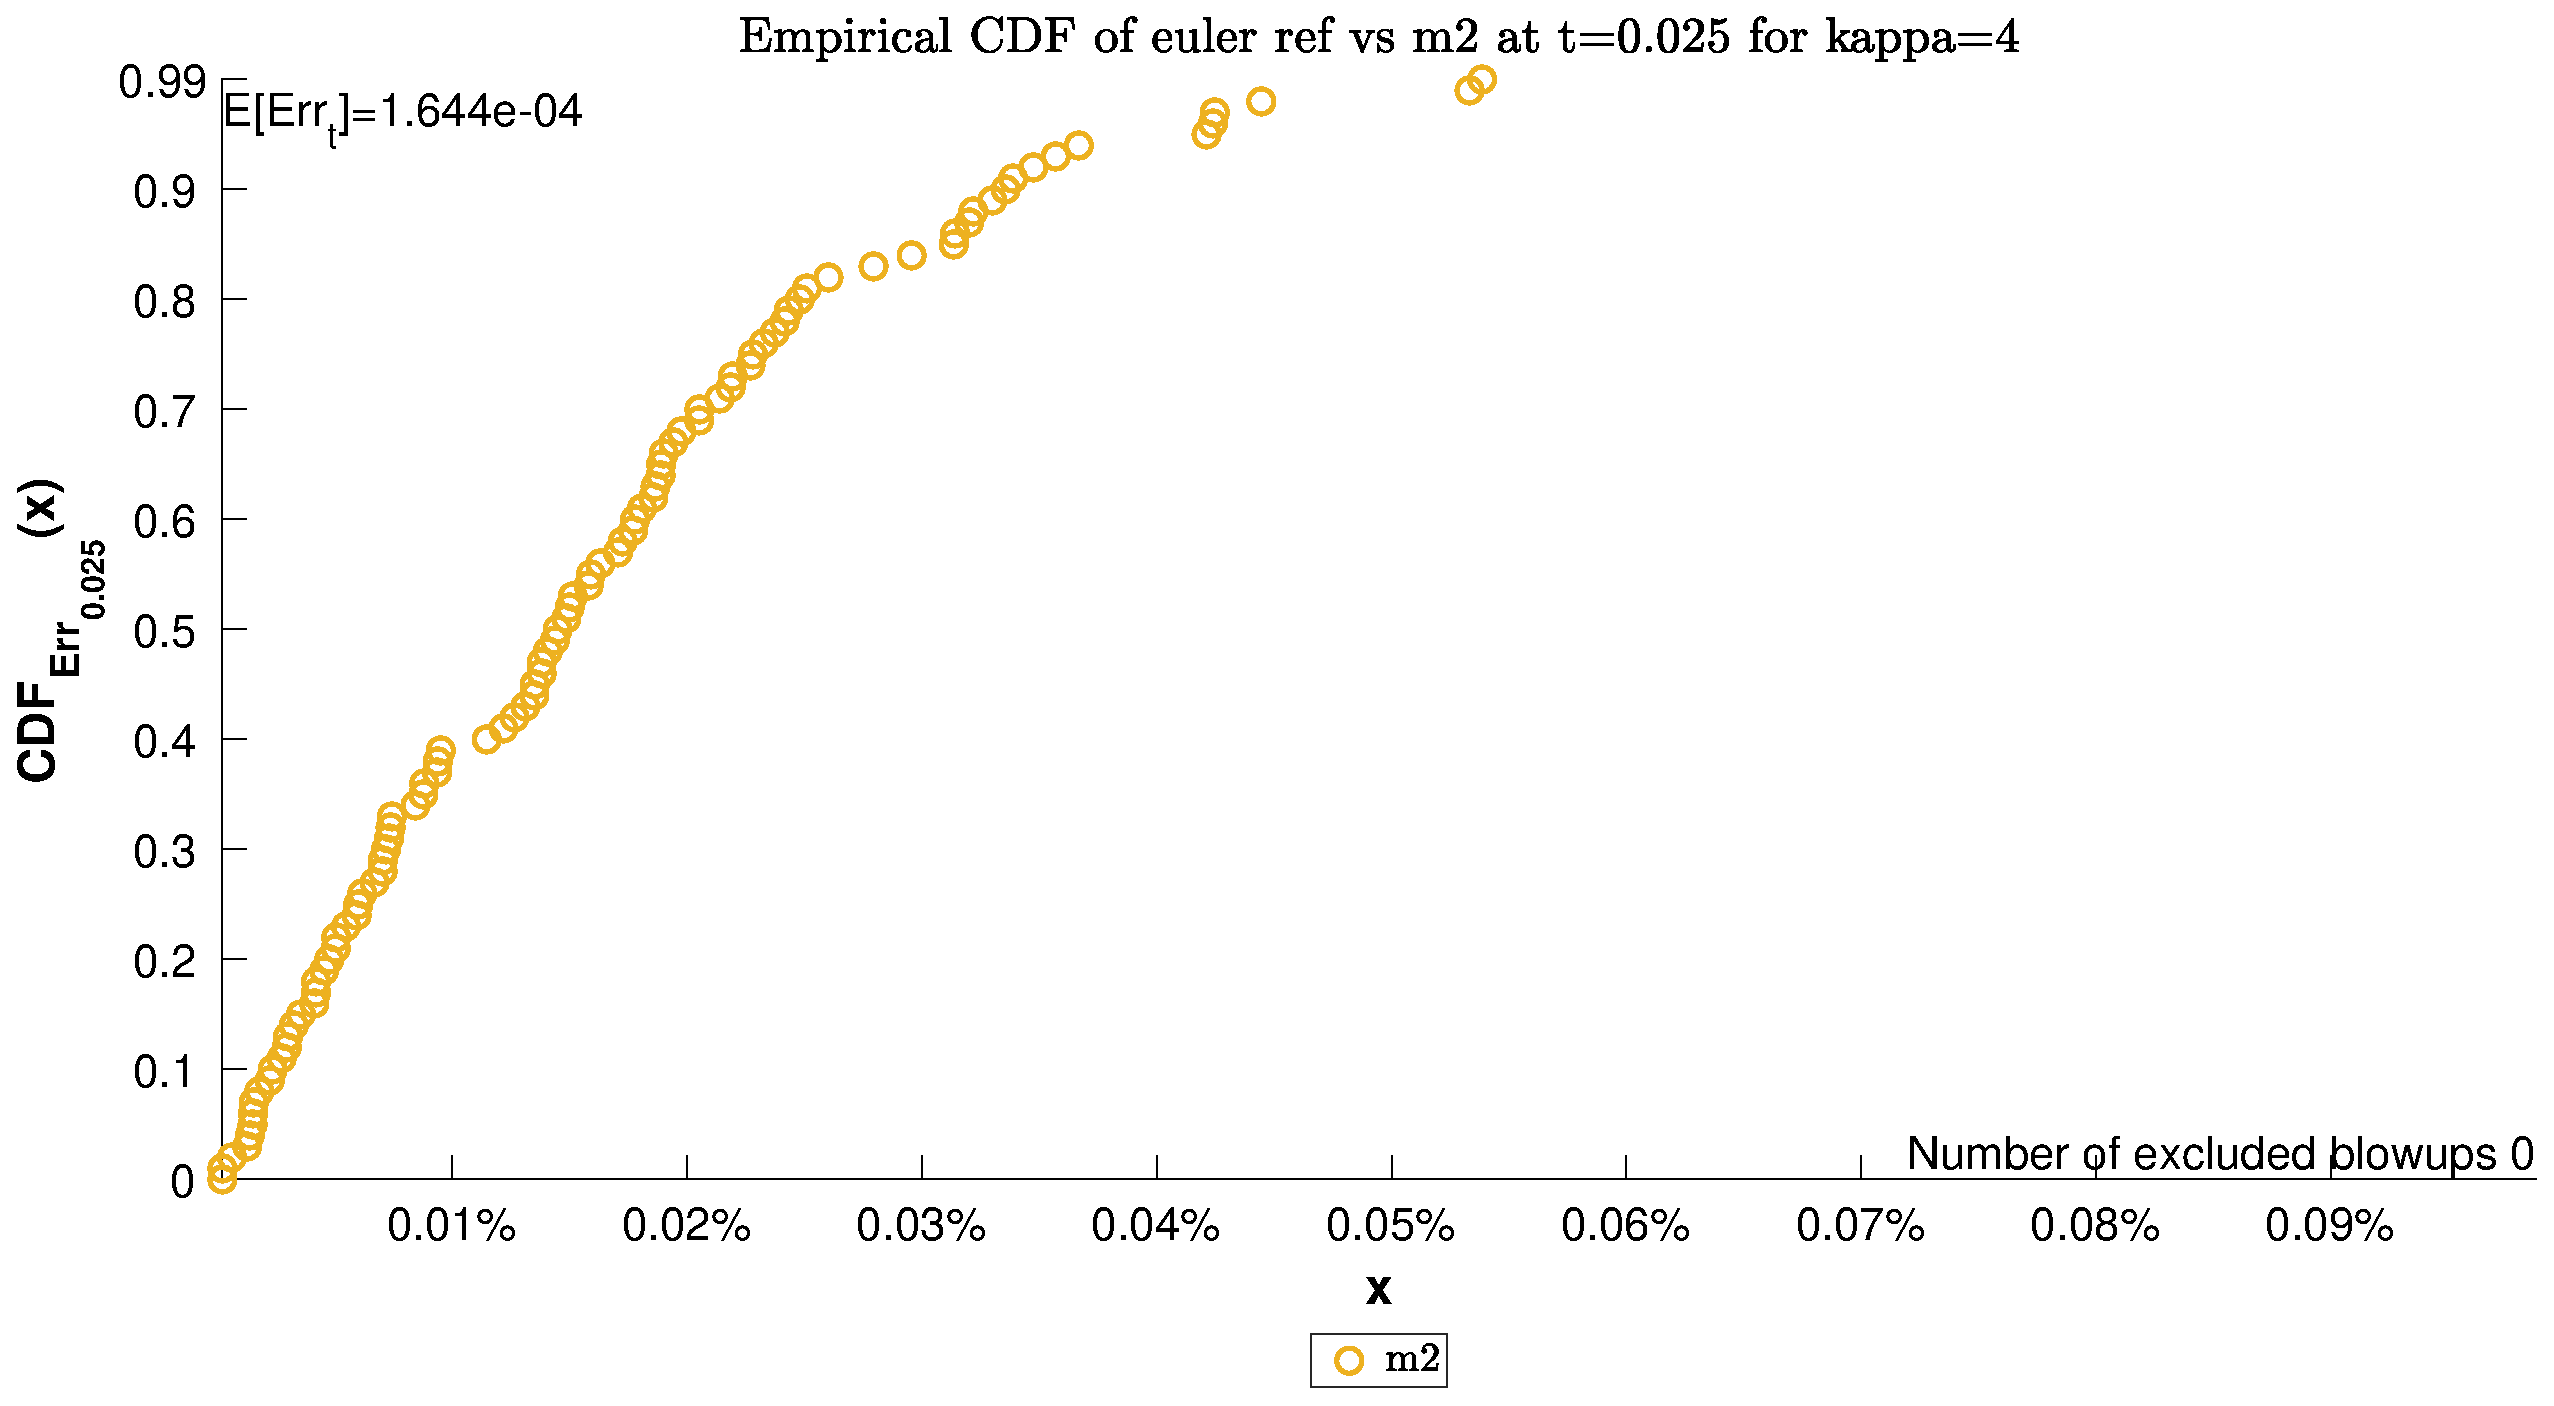
\includegraphics[width=.95\columnwidth]{CDF/CDFEulerRef_21}
\end{landscape}
\begin{landscape}
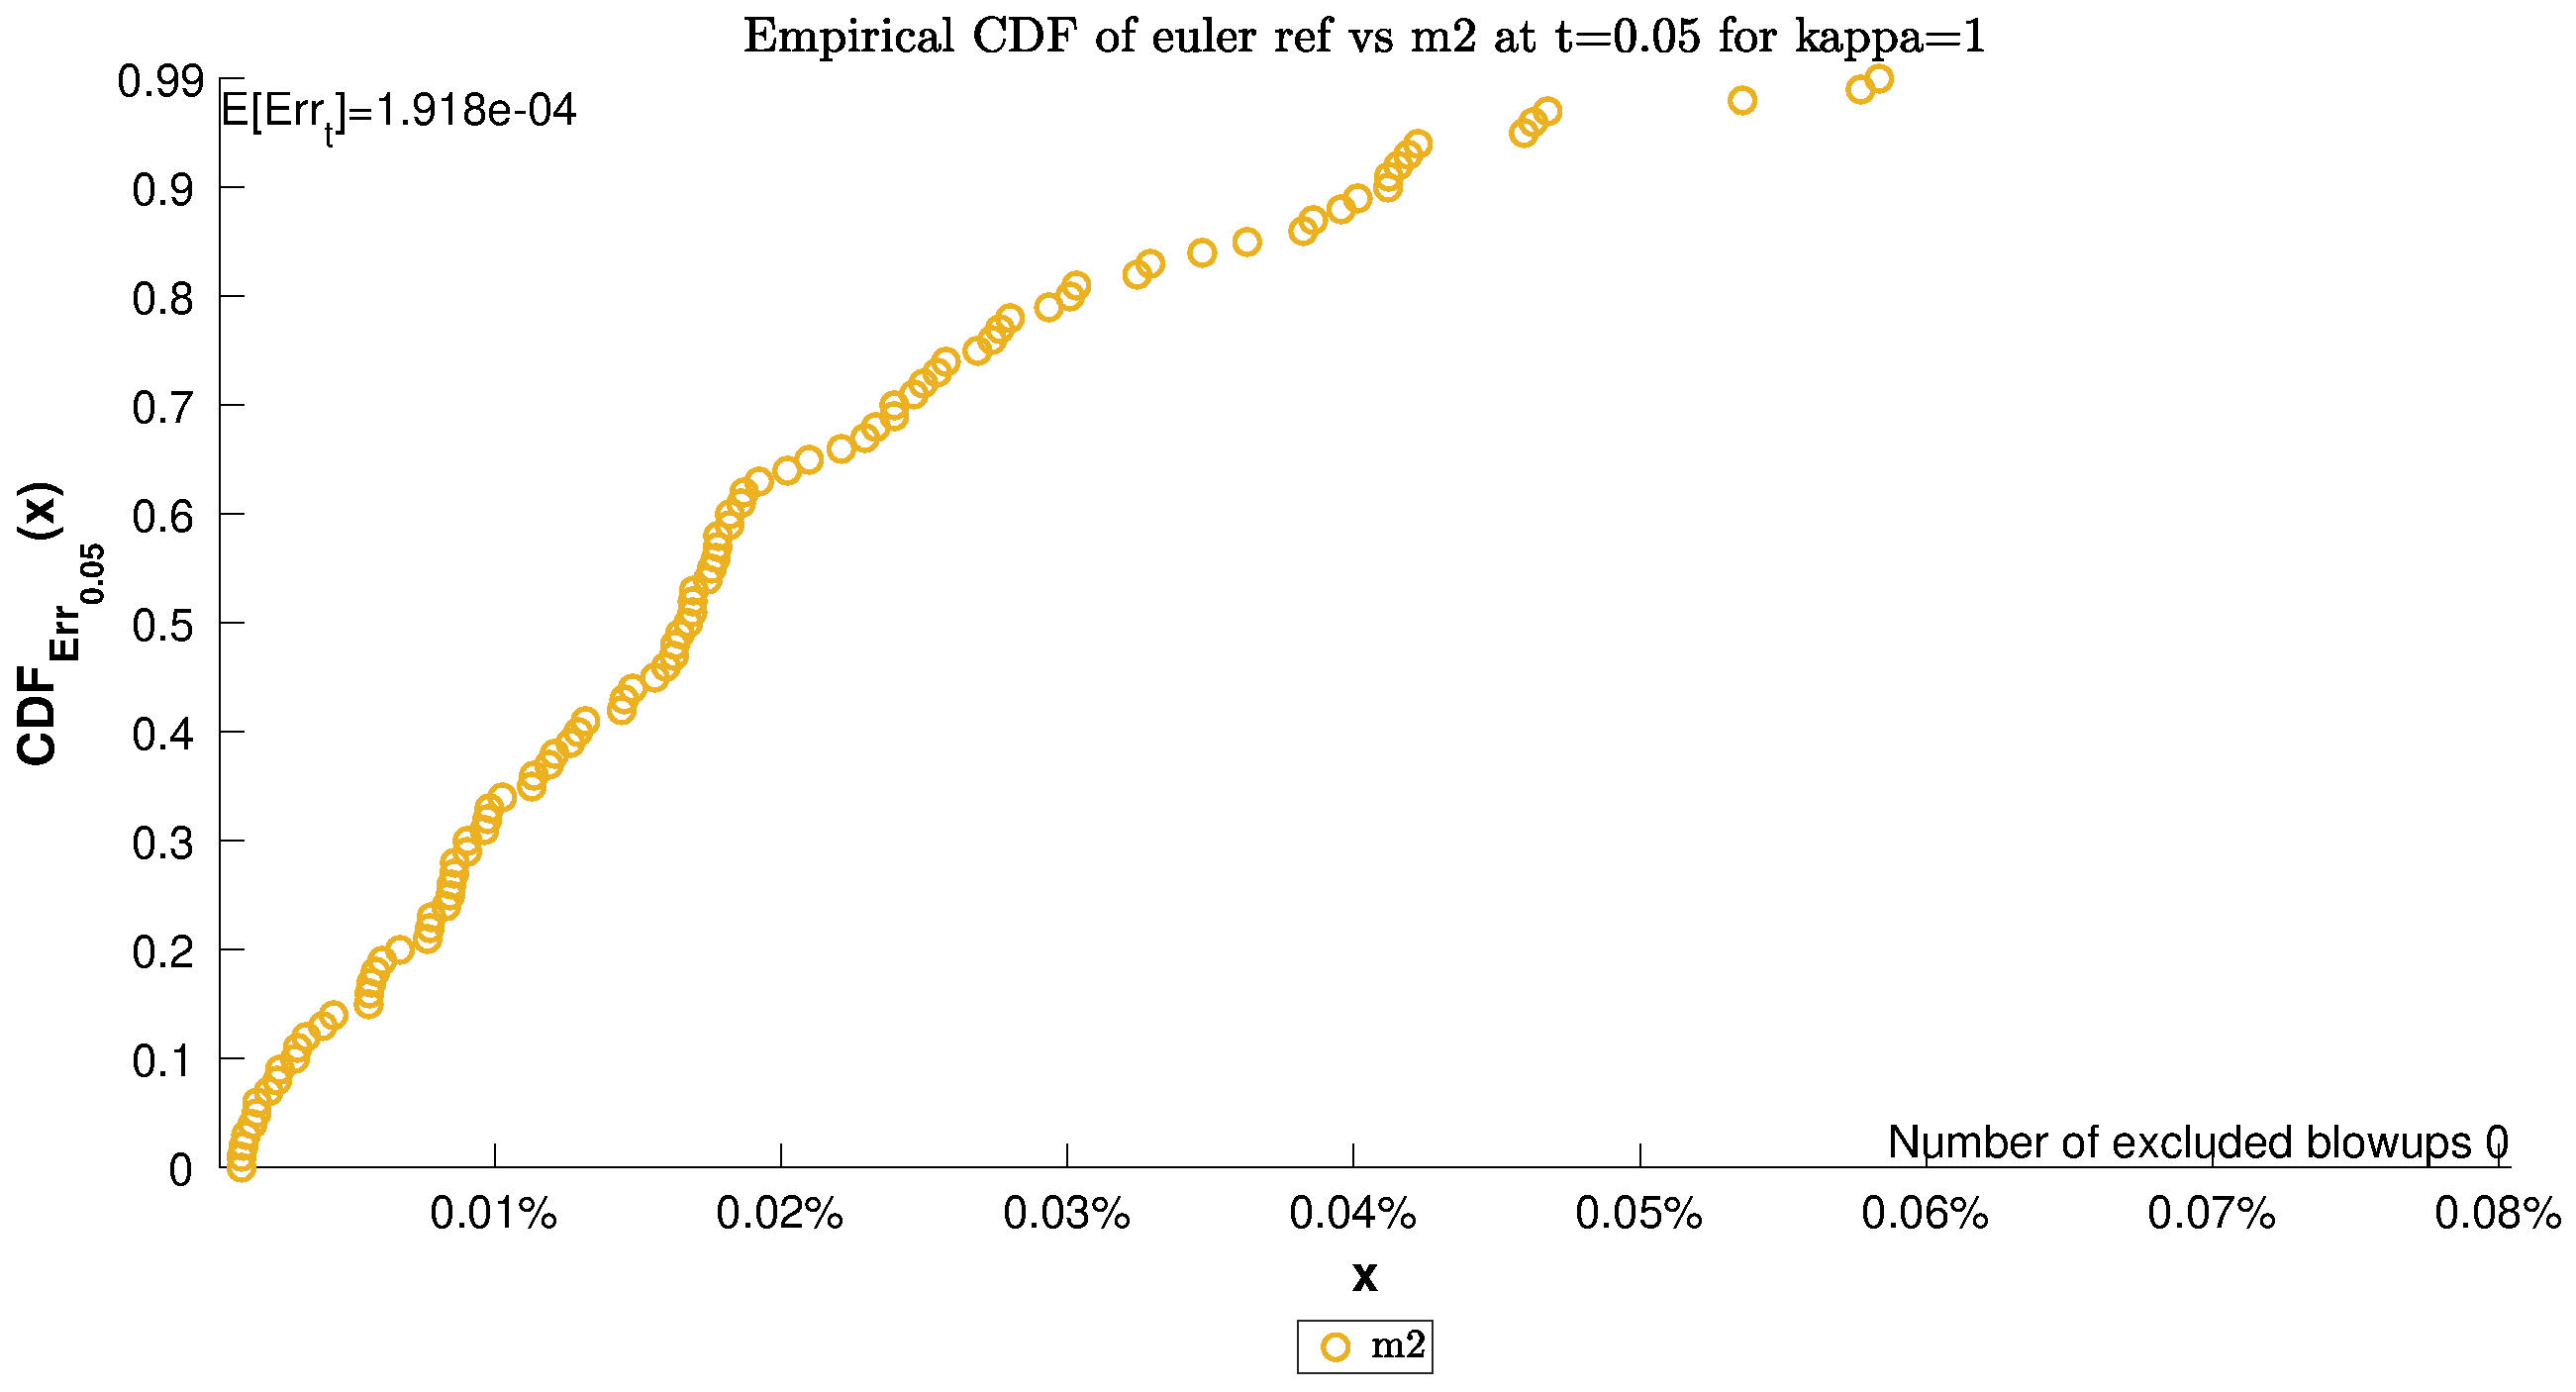
\includegraphics[width=.95\columnwidth]{CDF/CDFEulerRef_22}
\end{landscape}
\begin{landscape}
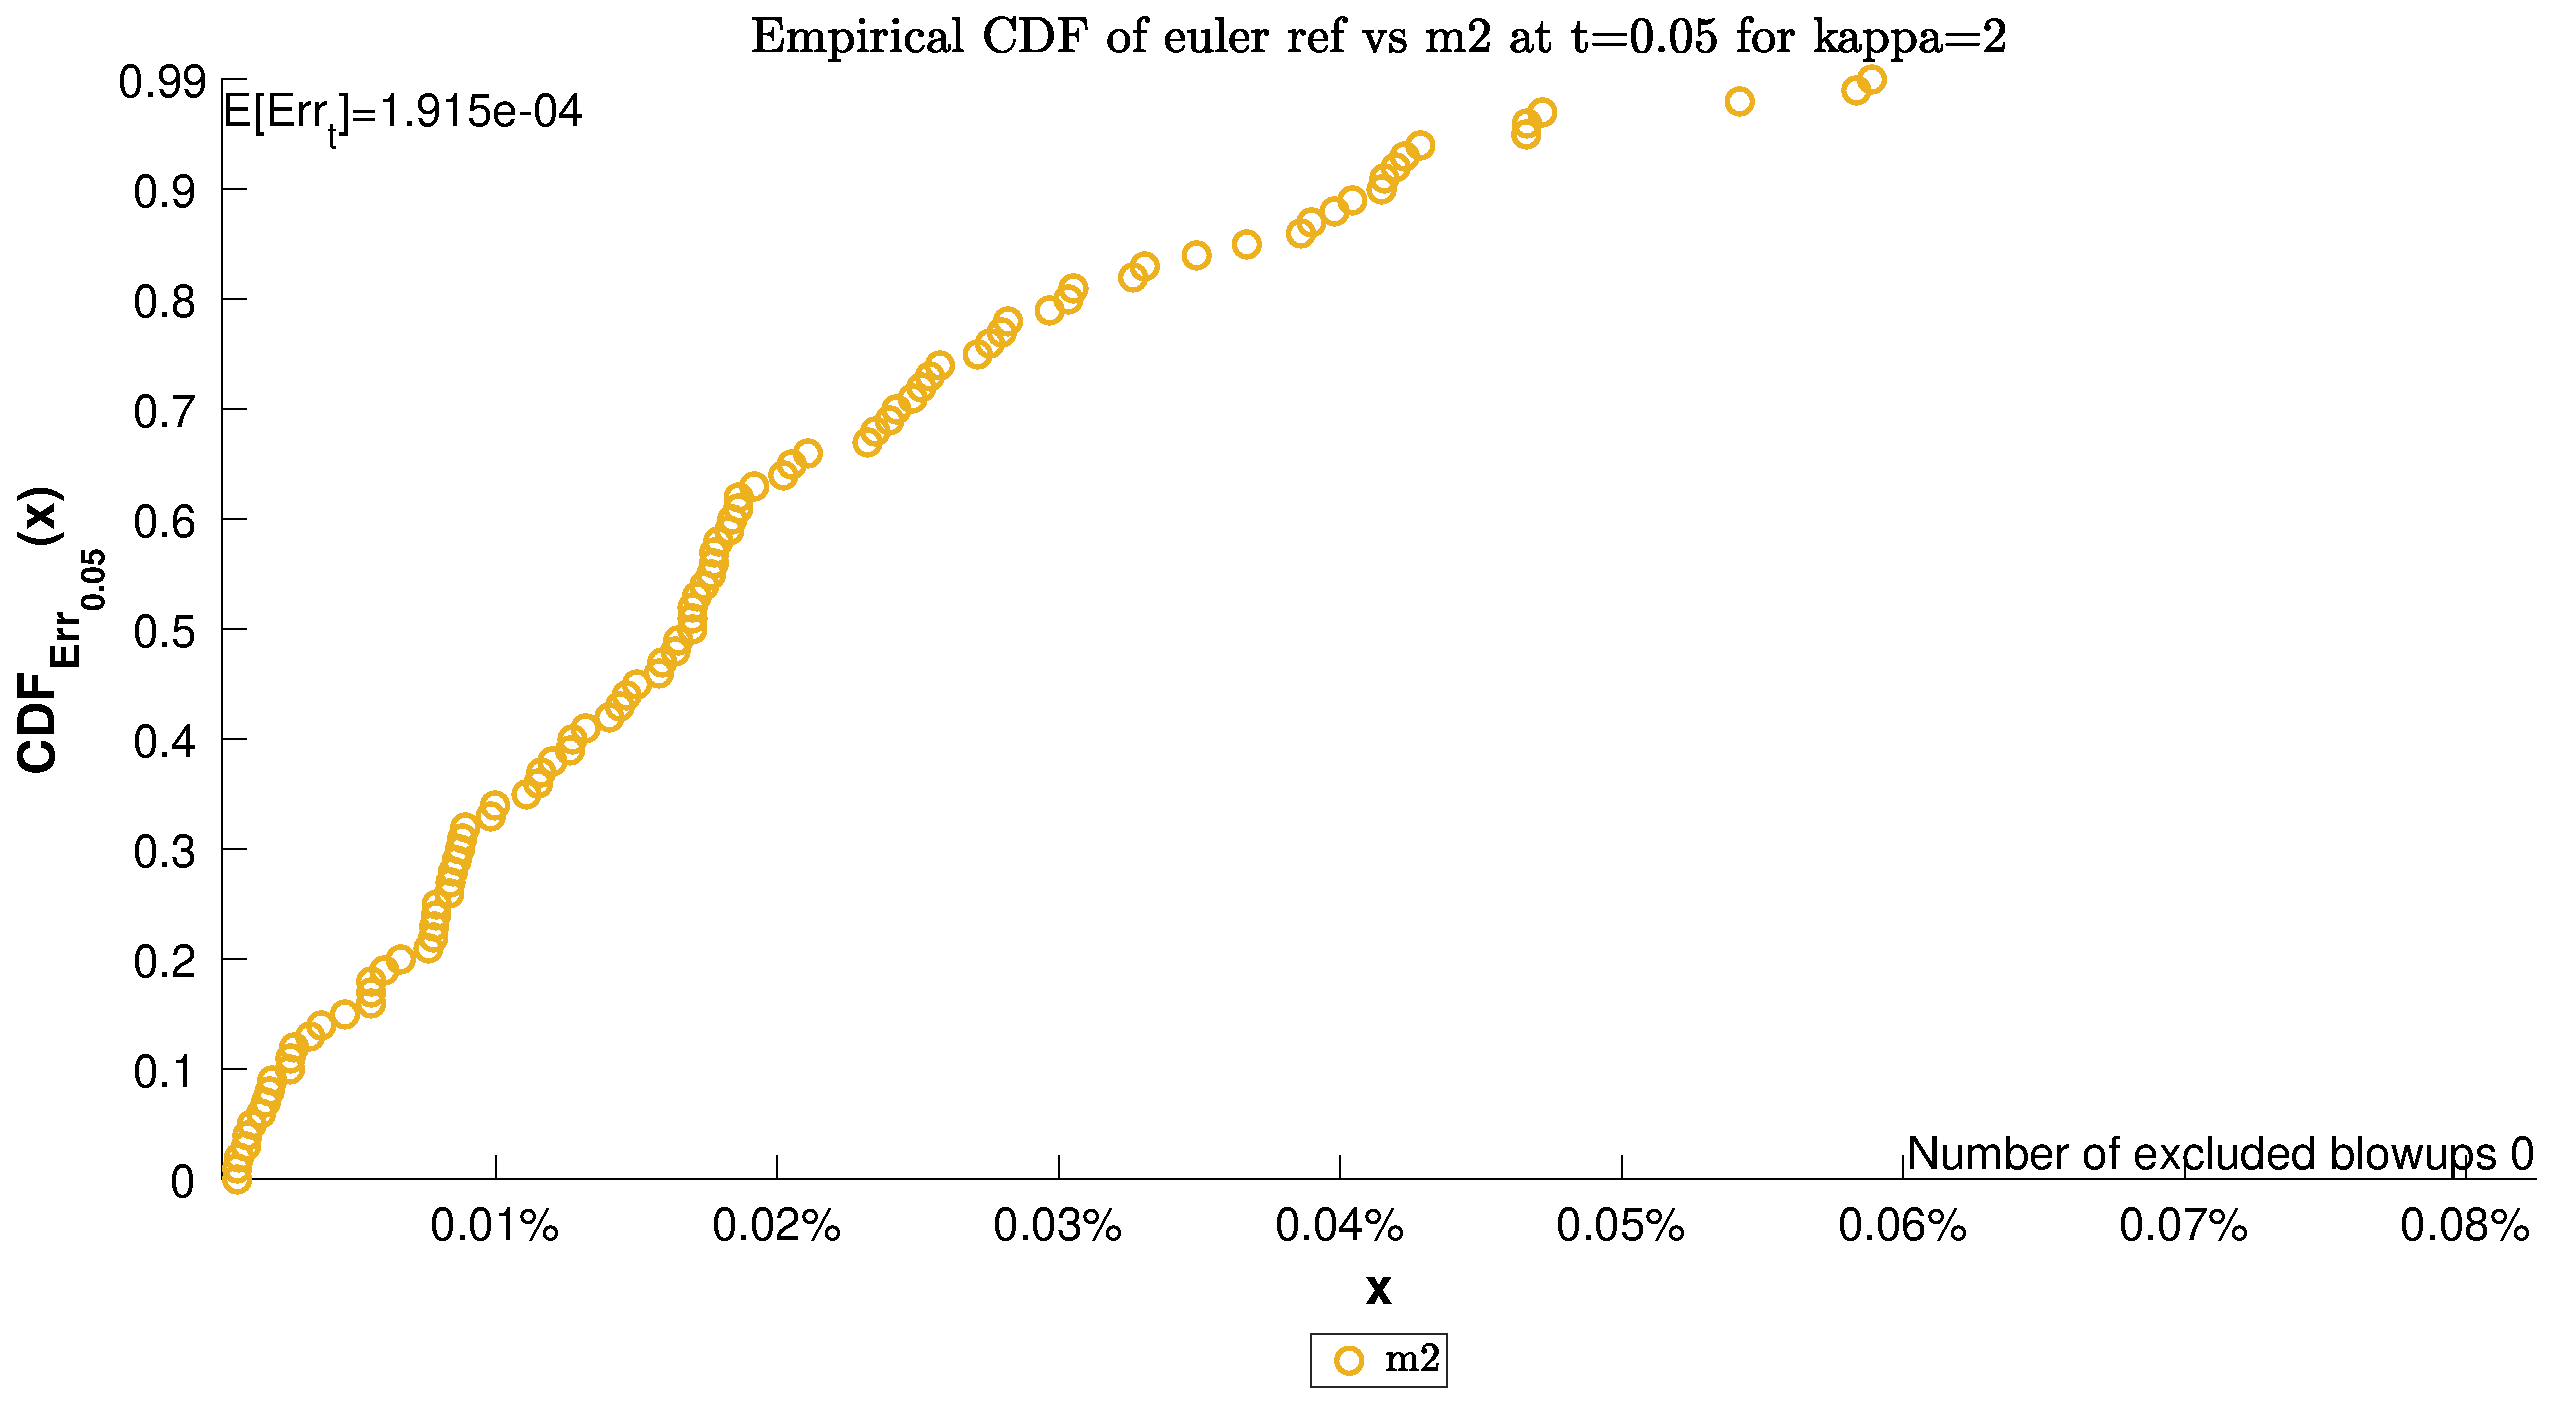
\includegraphics[width=.95\columnwidth]{CDF/CDFEulerRef_23}
\end{landscape}
\begin{landscape}
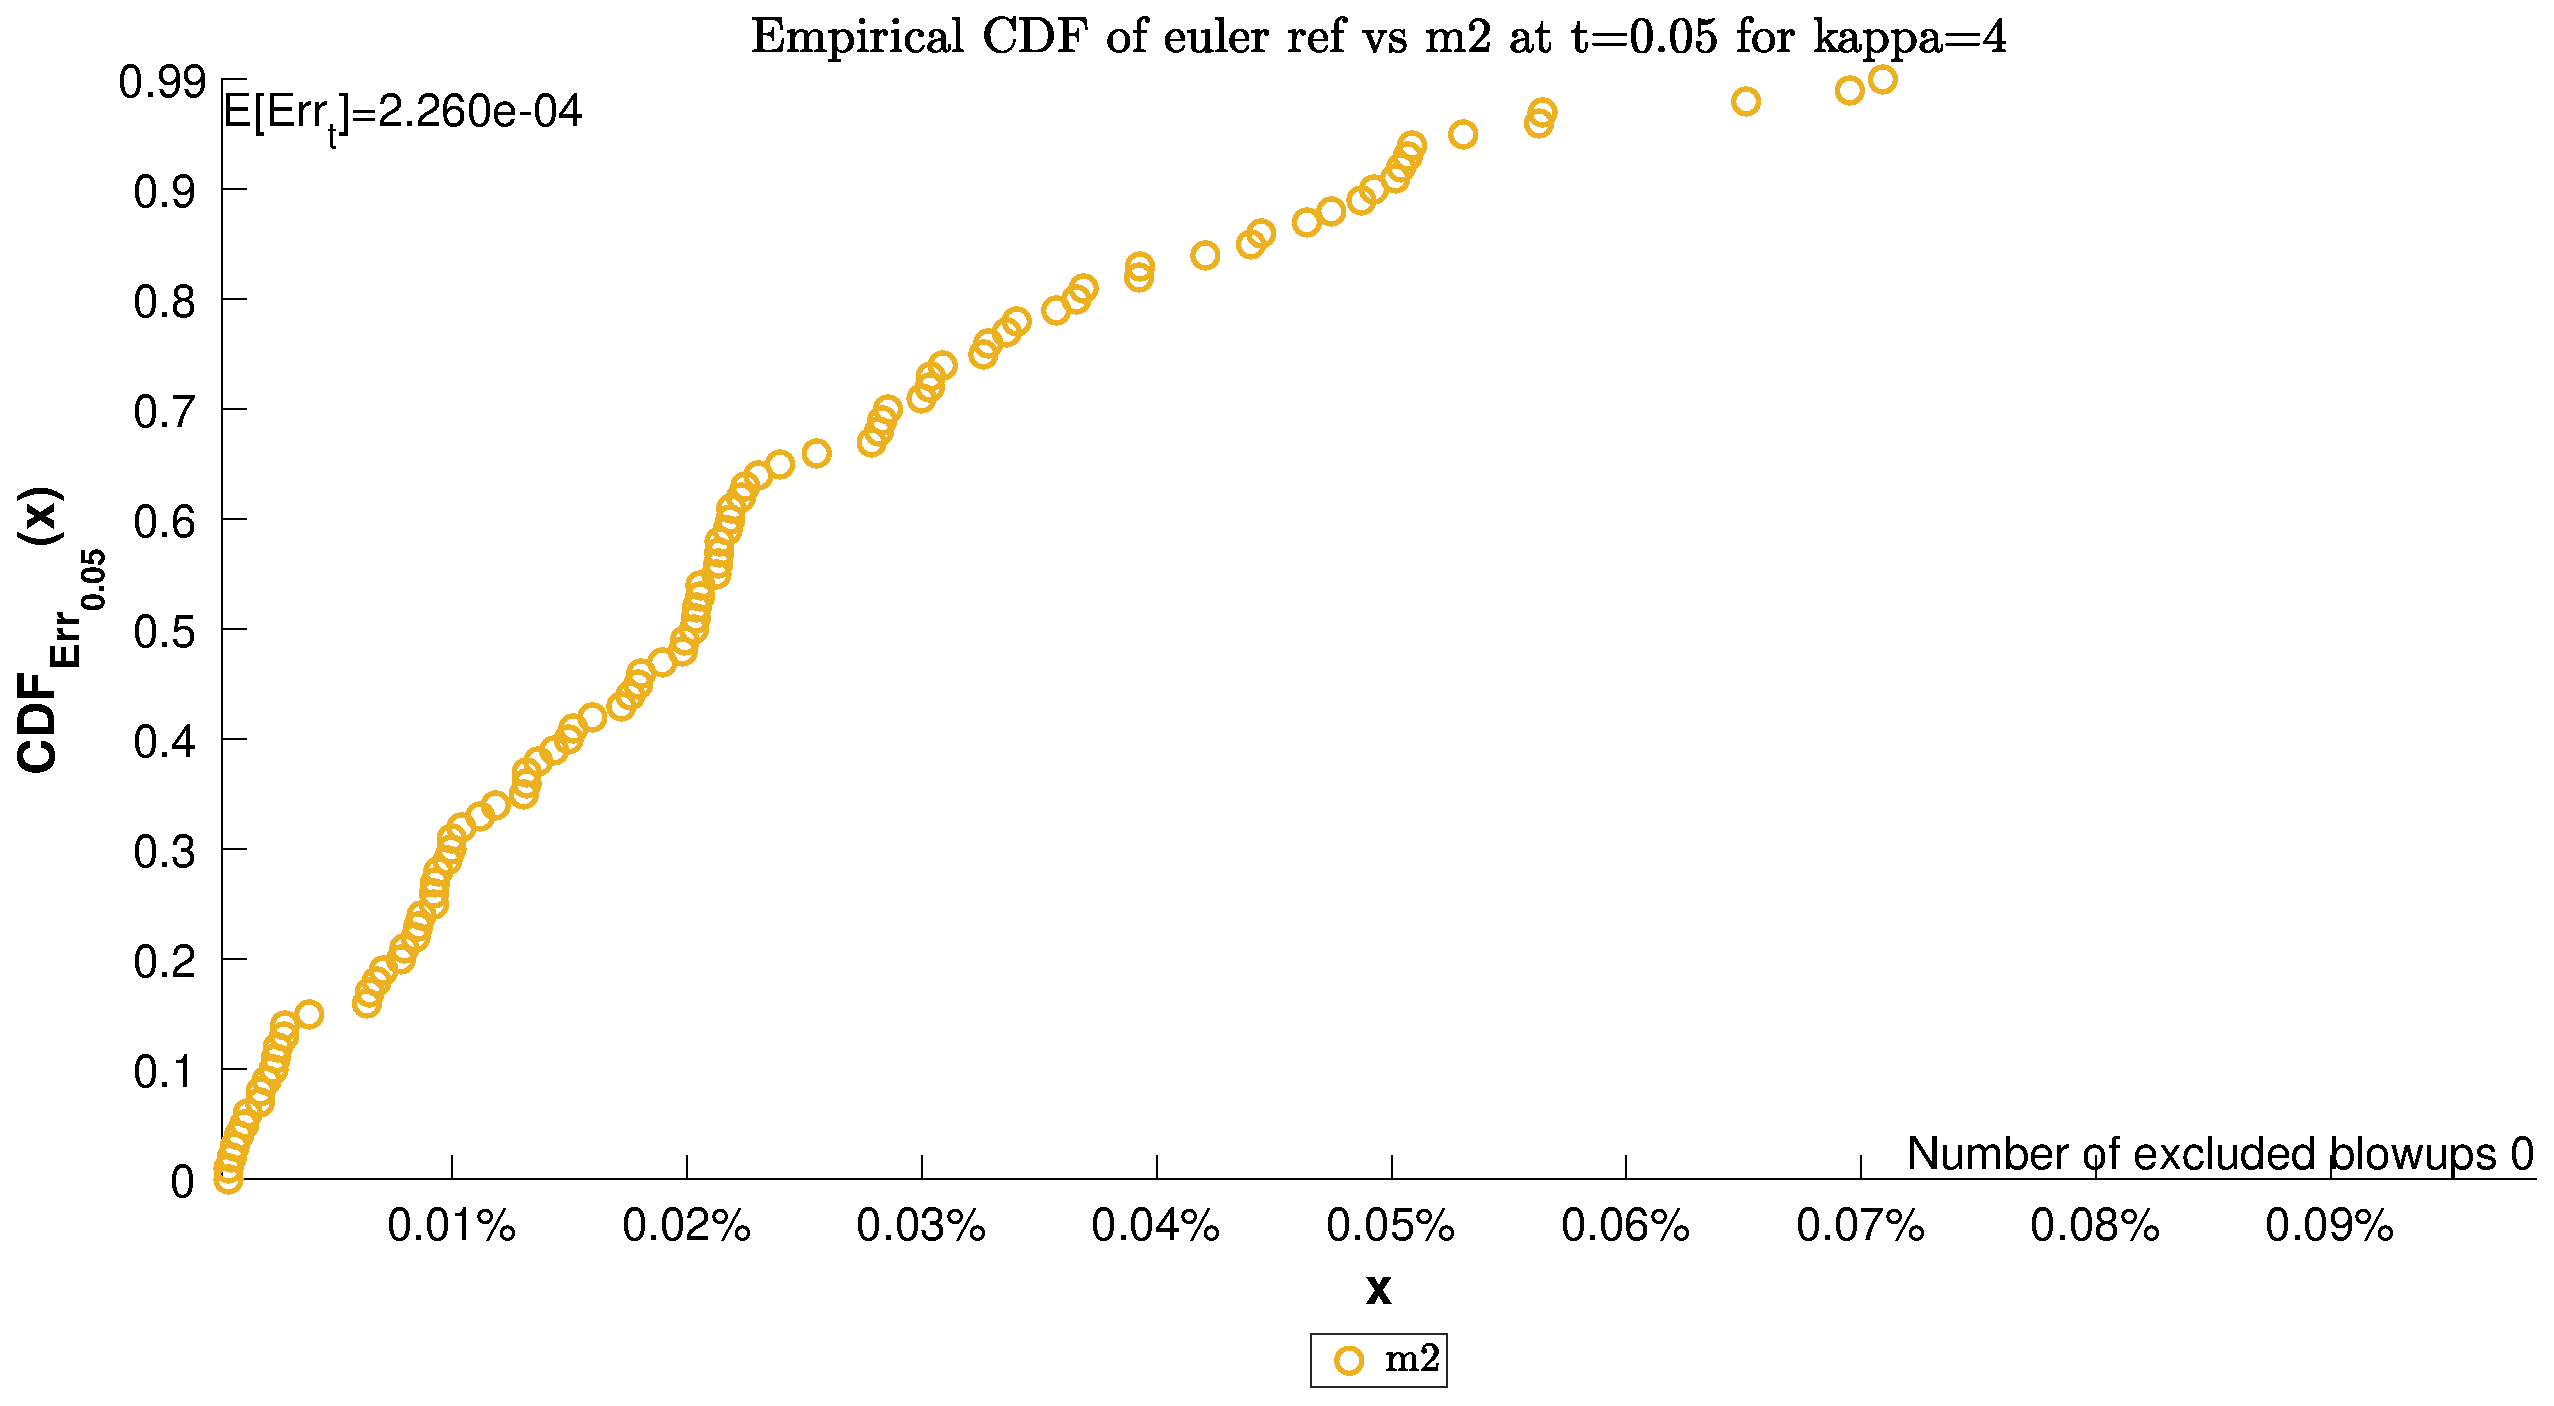
\includegraphics[width=.95\columnwidth]{CDF/CDFEulerRef_24}
\end{landscape}
\begin{landscape}
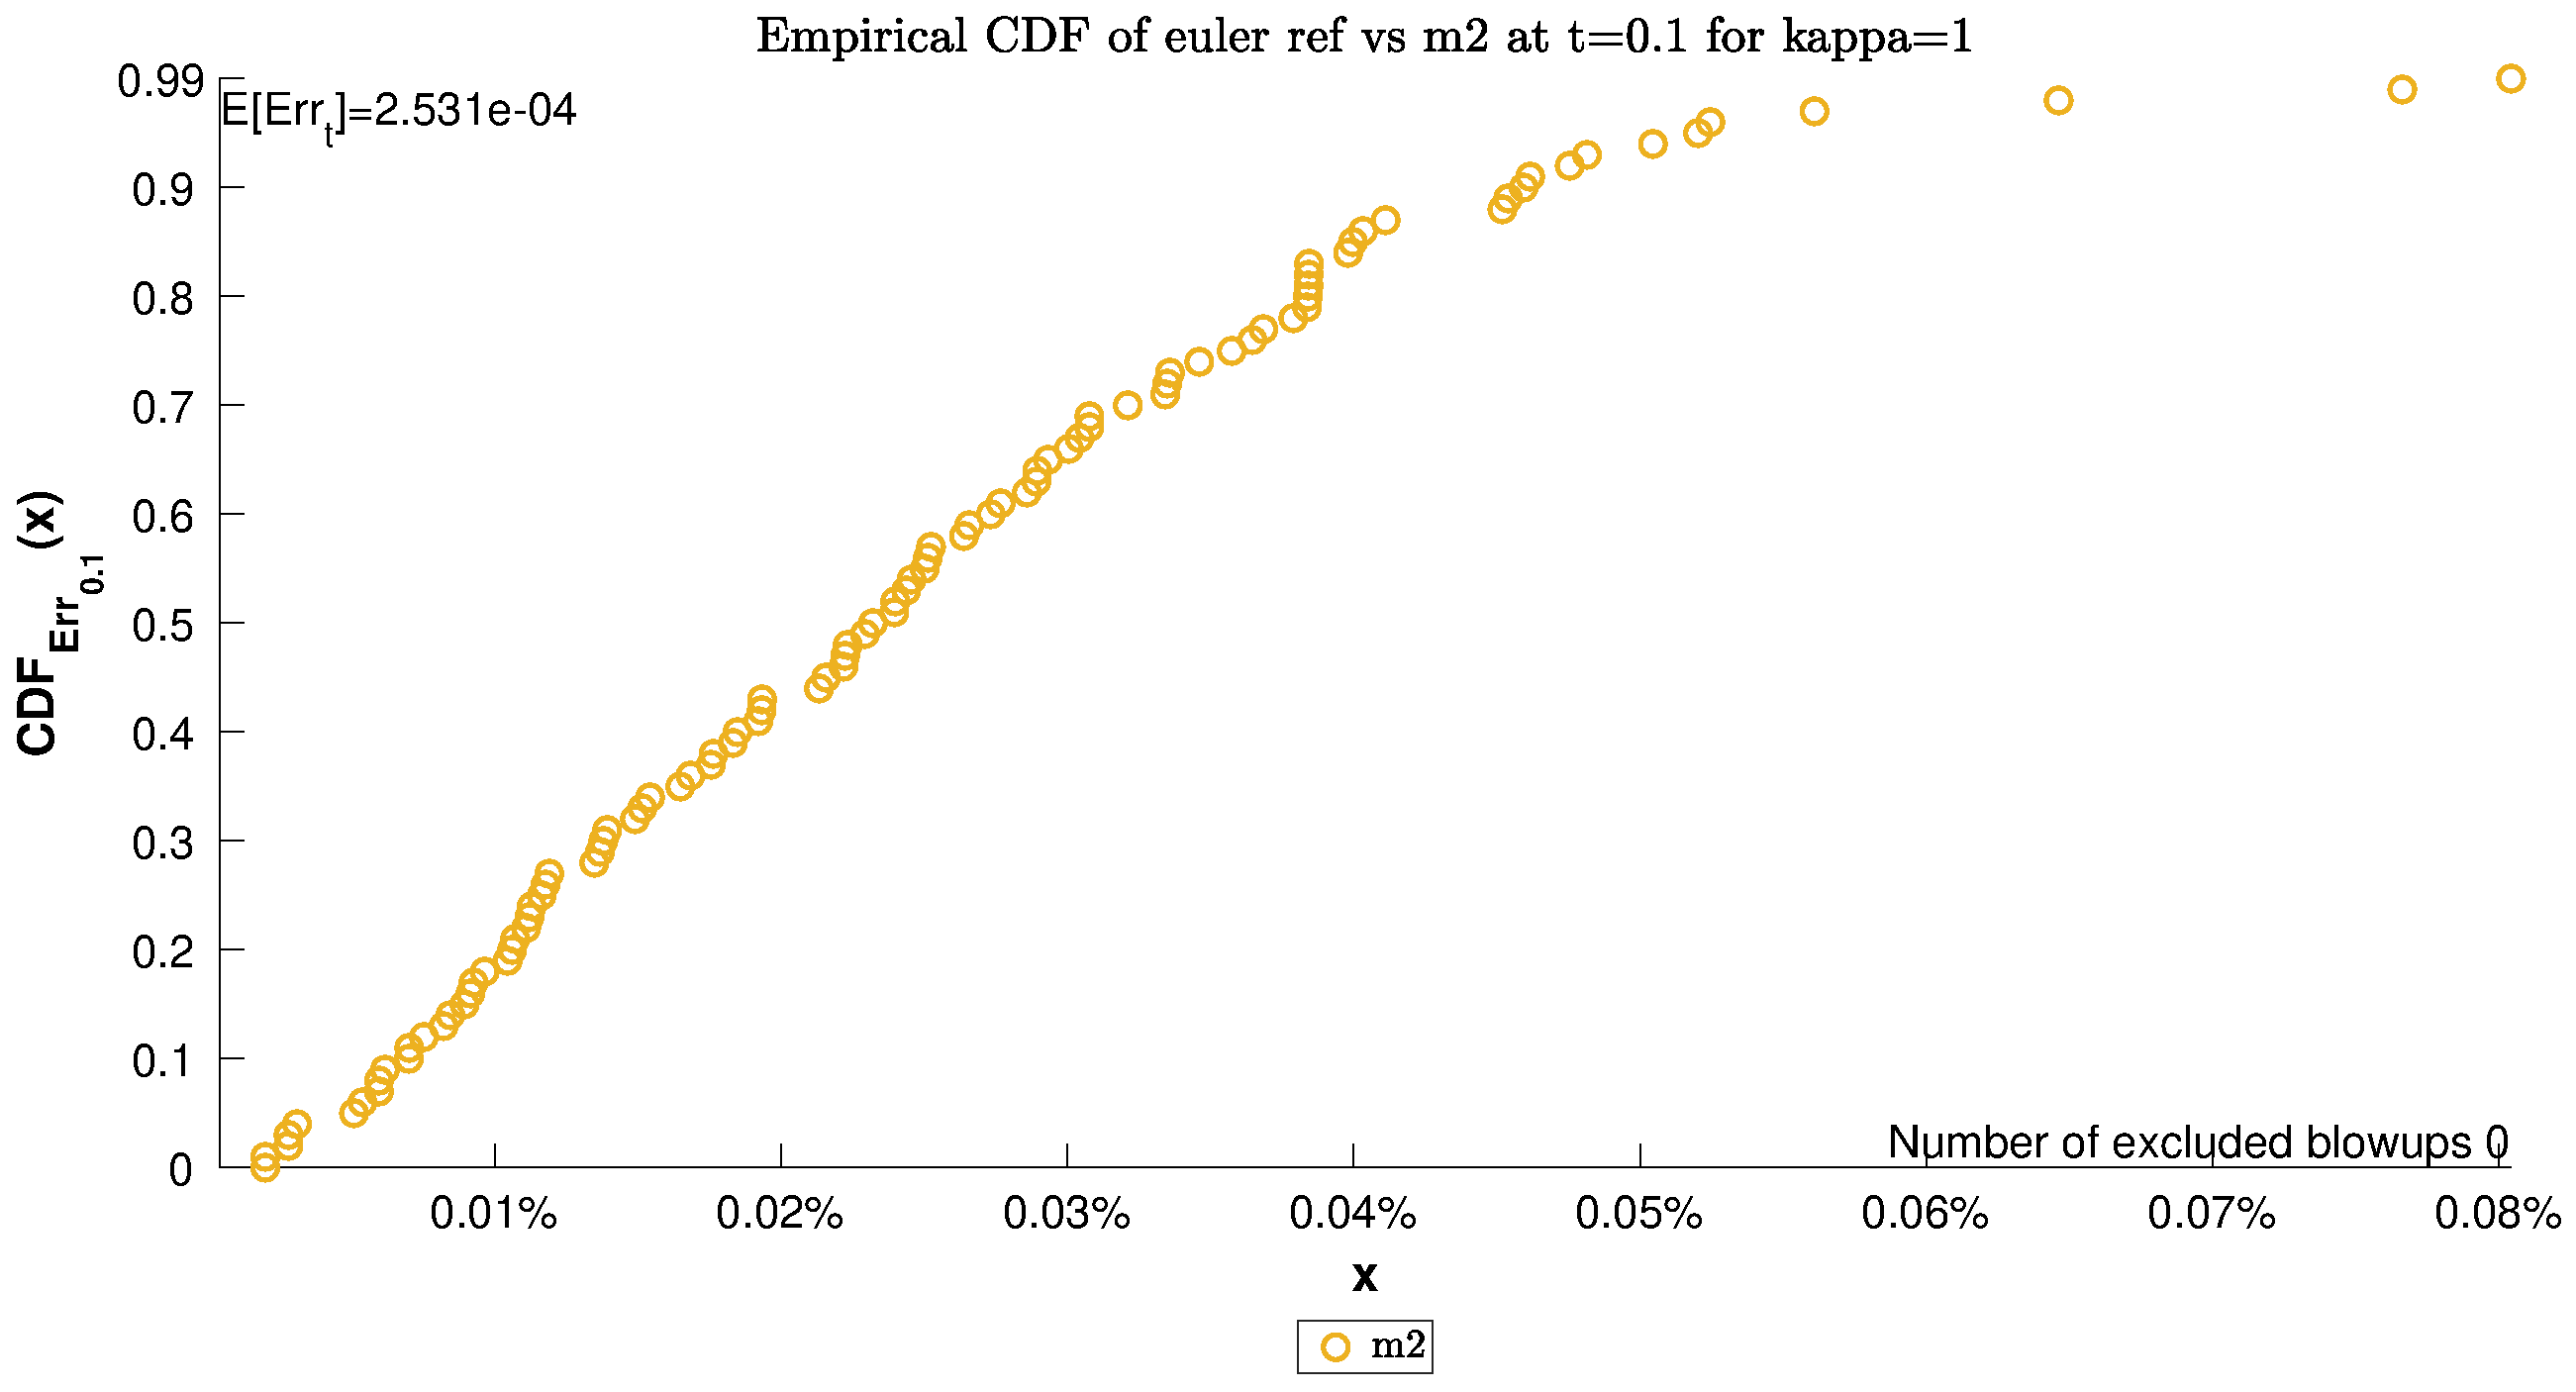
\includegraphics[width=.95\columnwidth]{CDF/CDFEulerRef_25}
\end{landscape}
\begin{landscape}
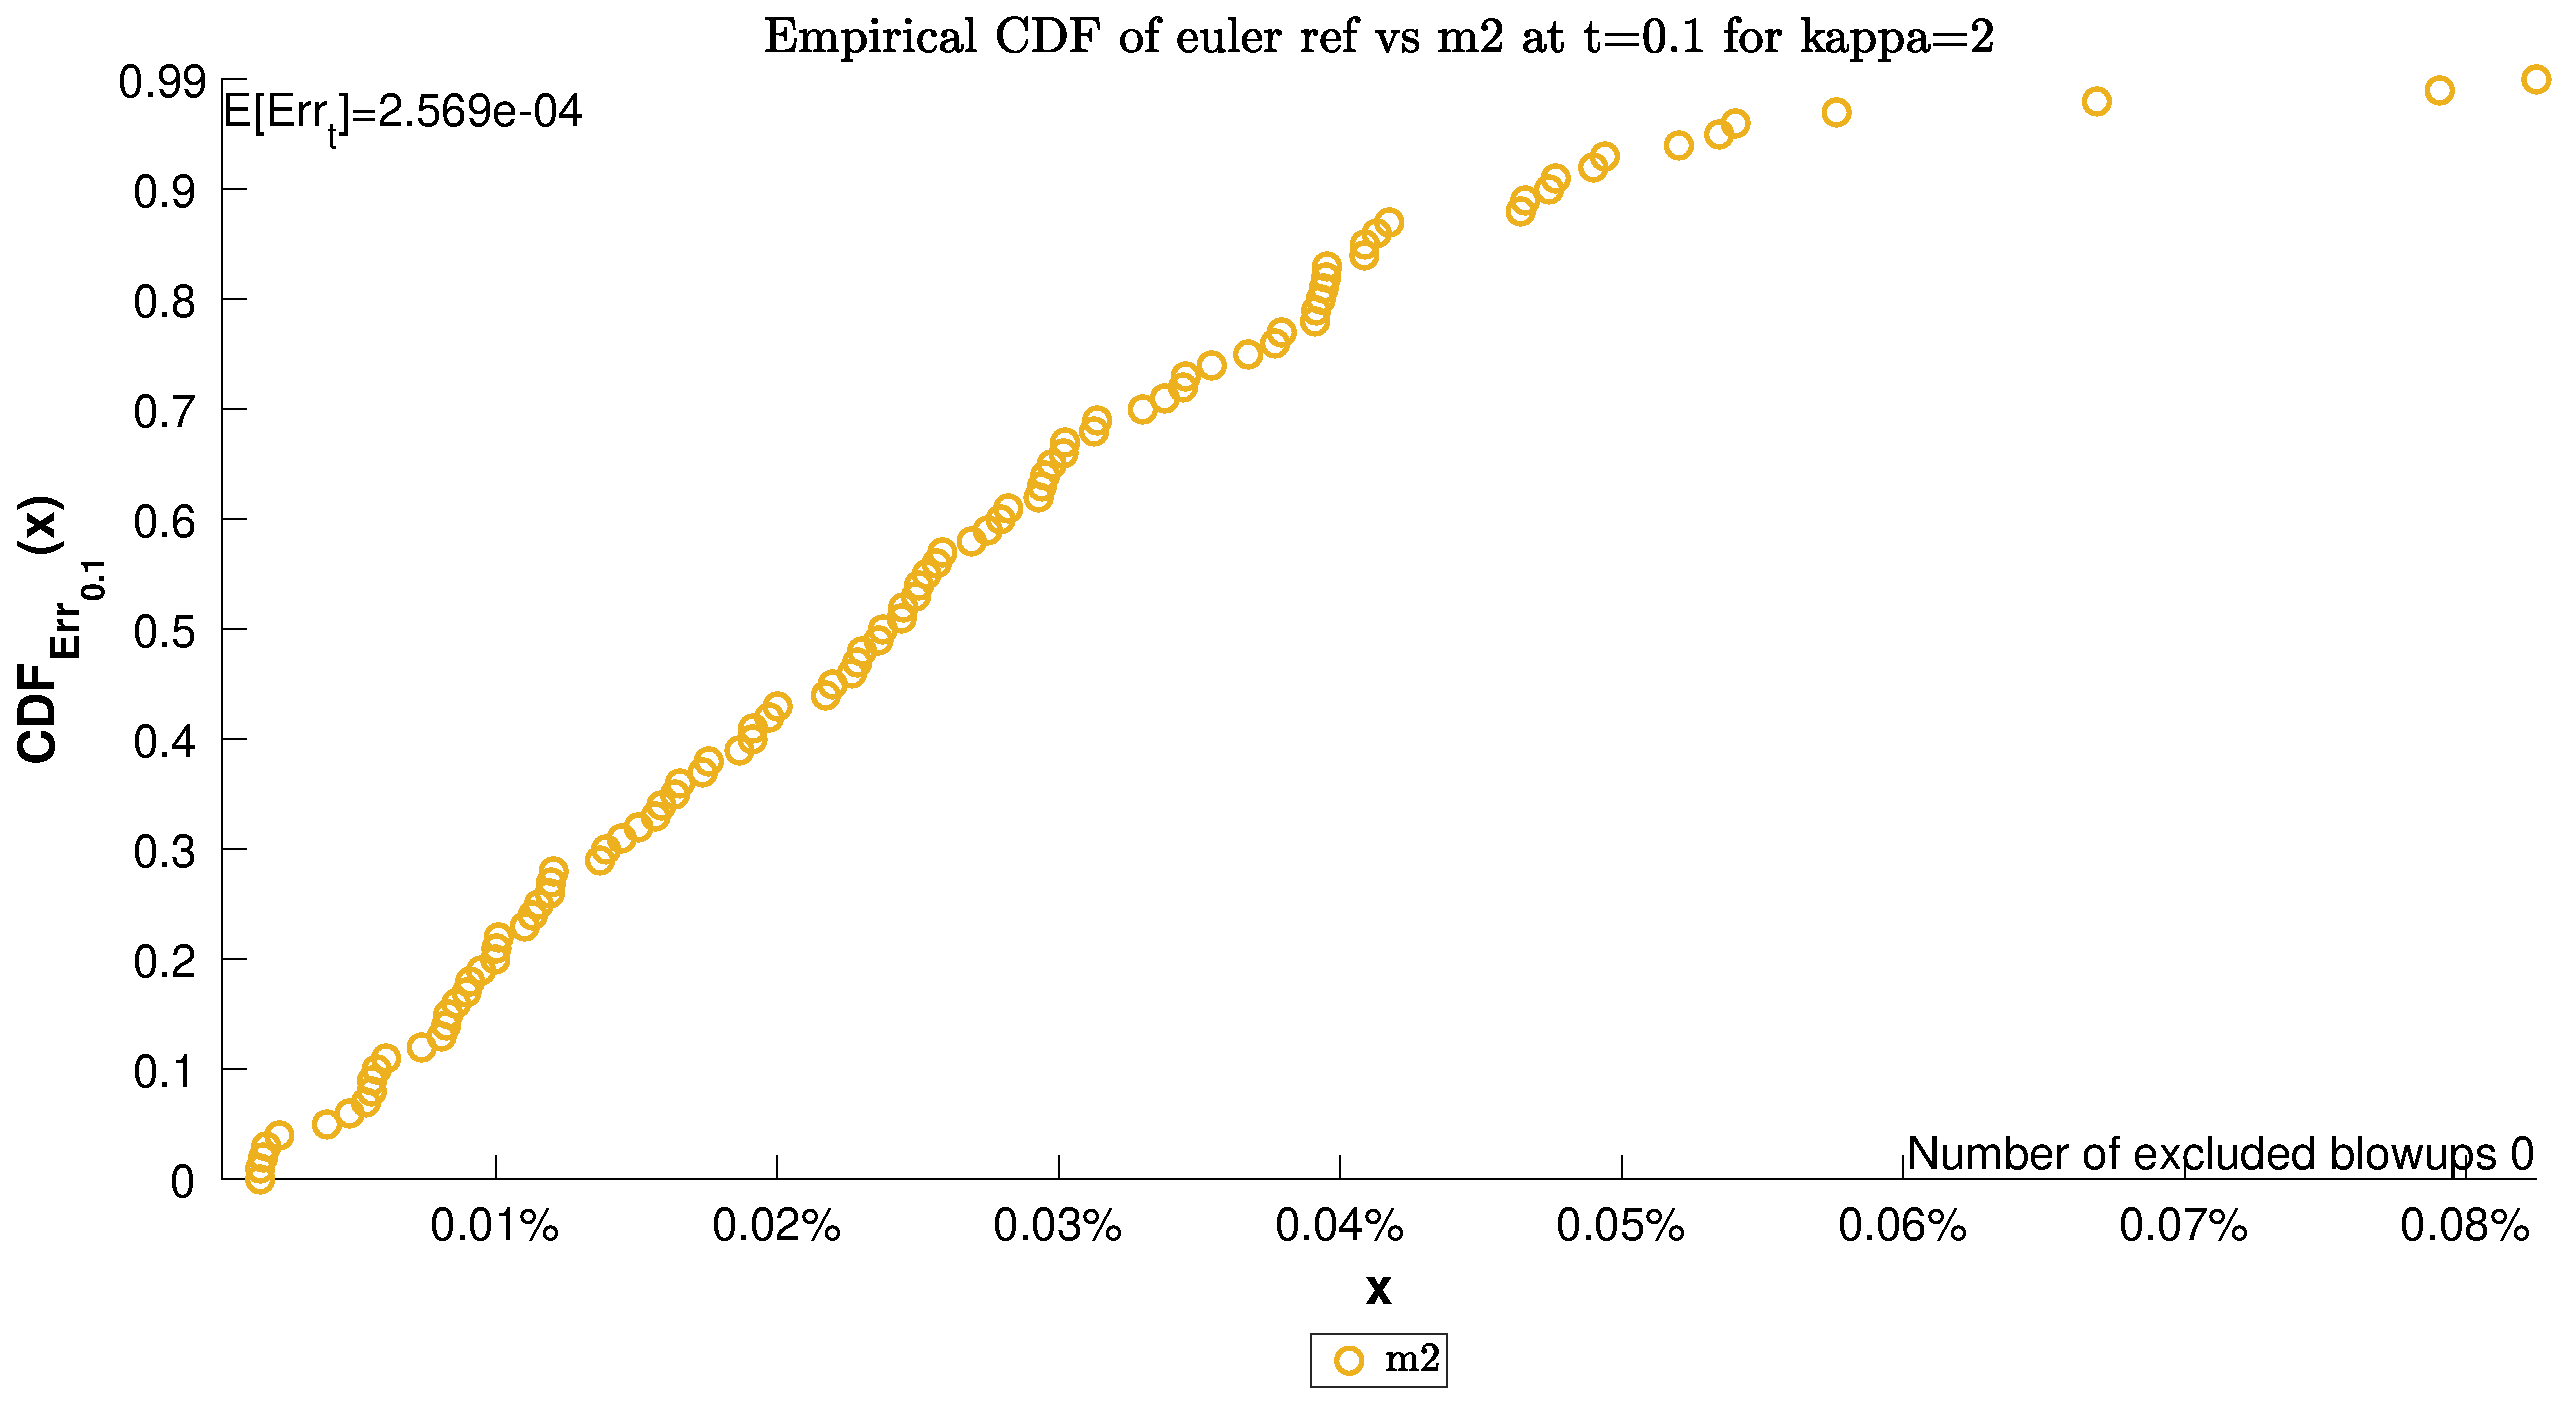
\includegraphics[width=.95\columnwidth]{CDF/CDFEulerRef_26}
\end{landscape}
\begin{landscape}
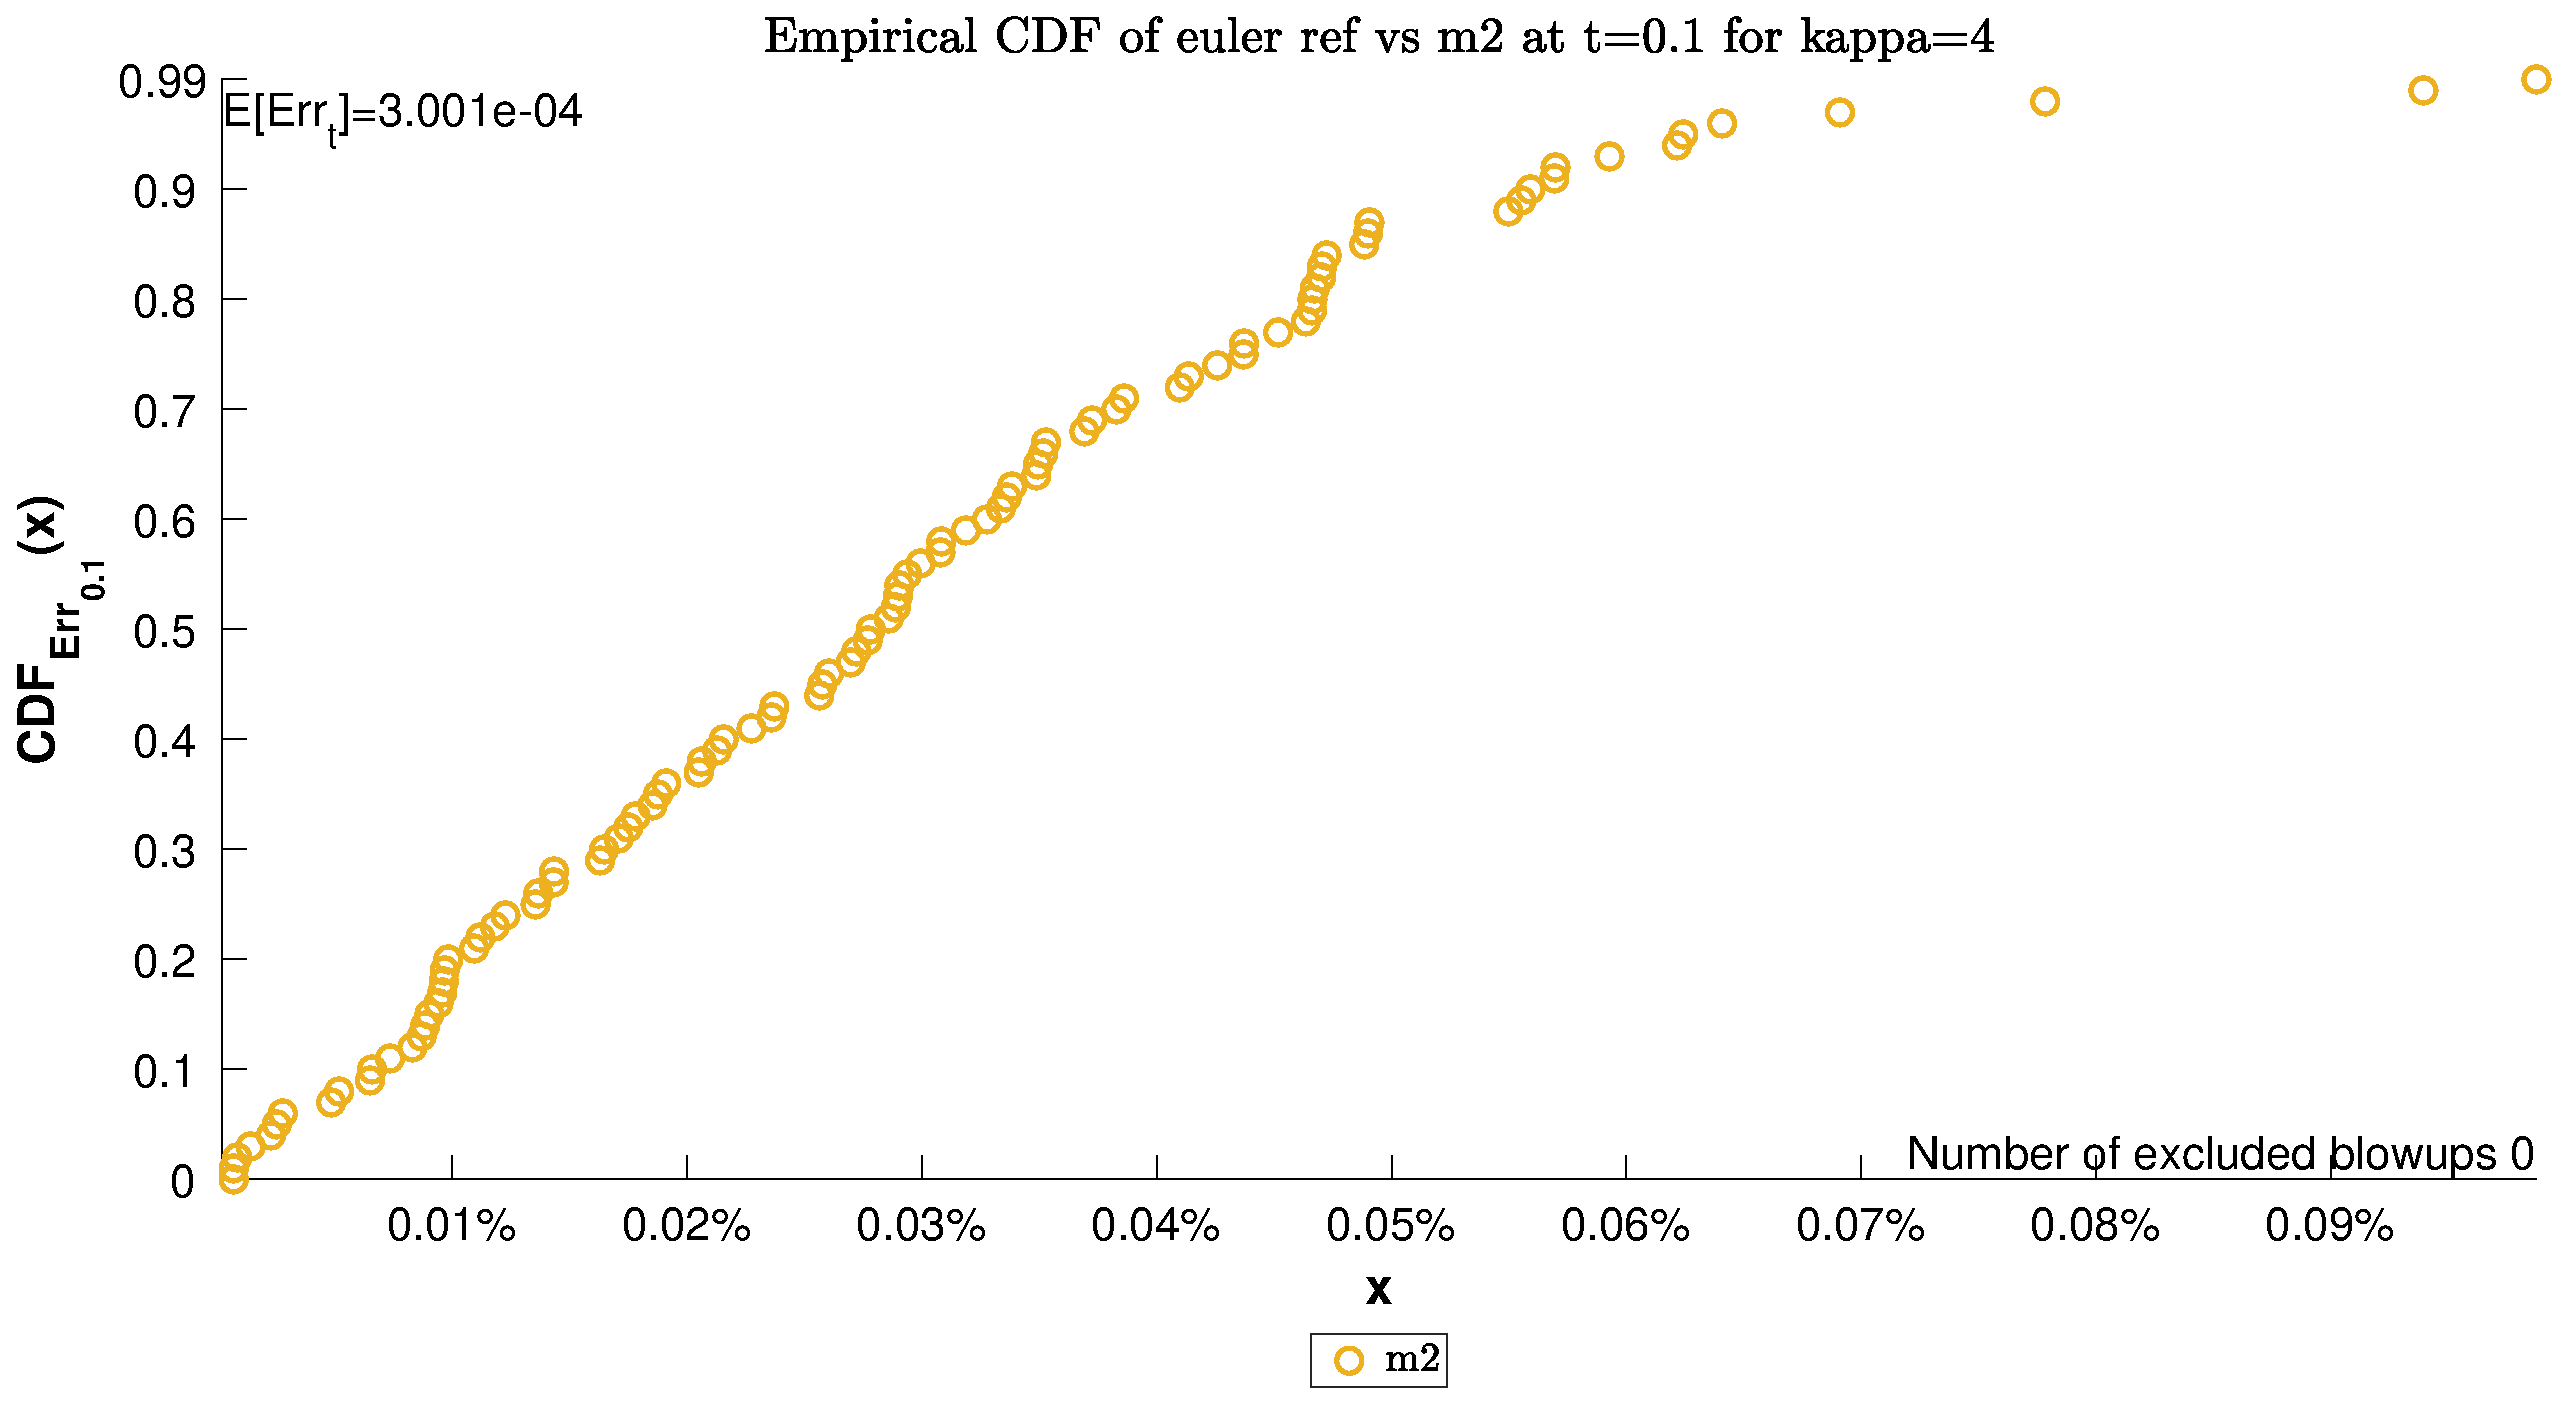
\includegraphics[width=.95\columnwidth]{CDF/CDFEulerRef_27}
\end{landscape}
\begin{landscape}
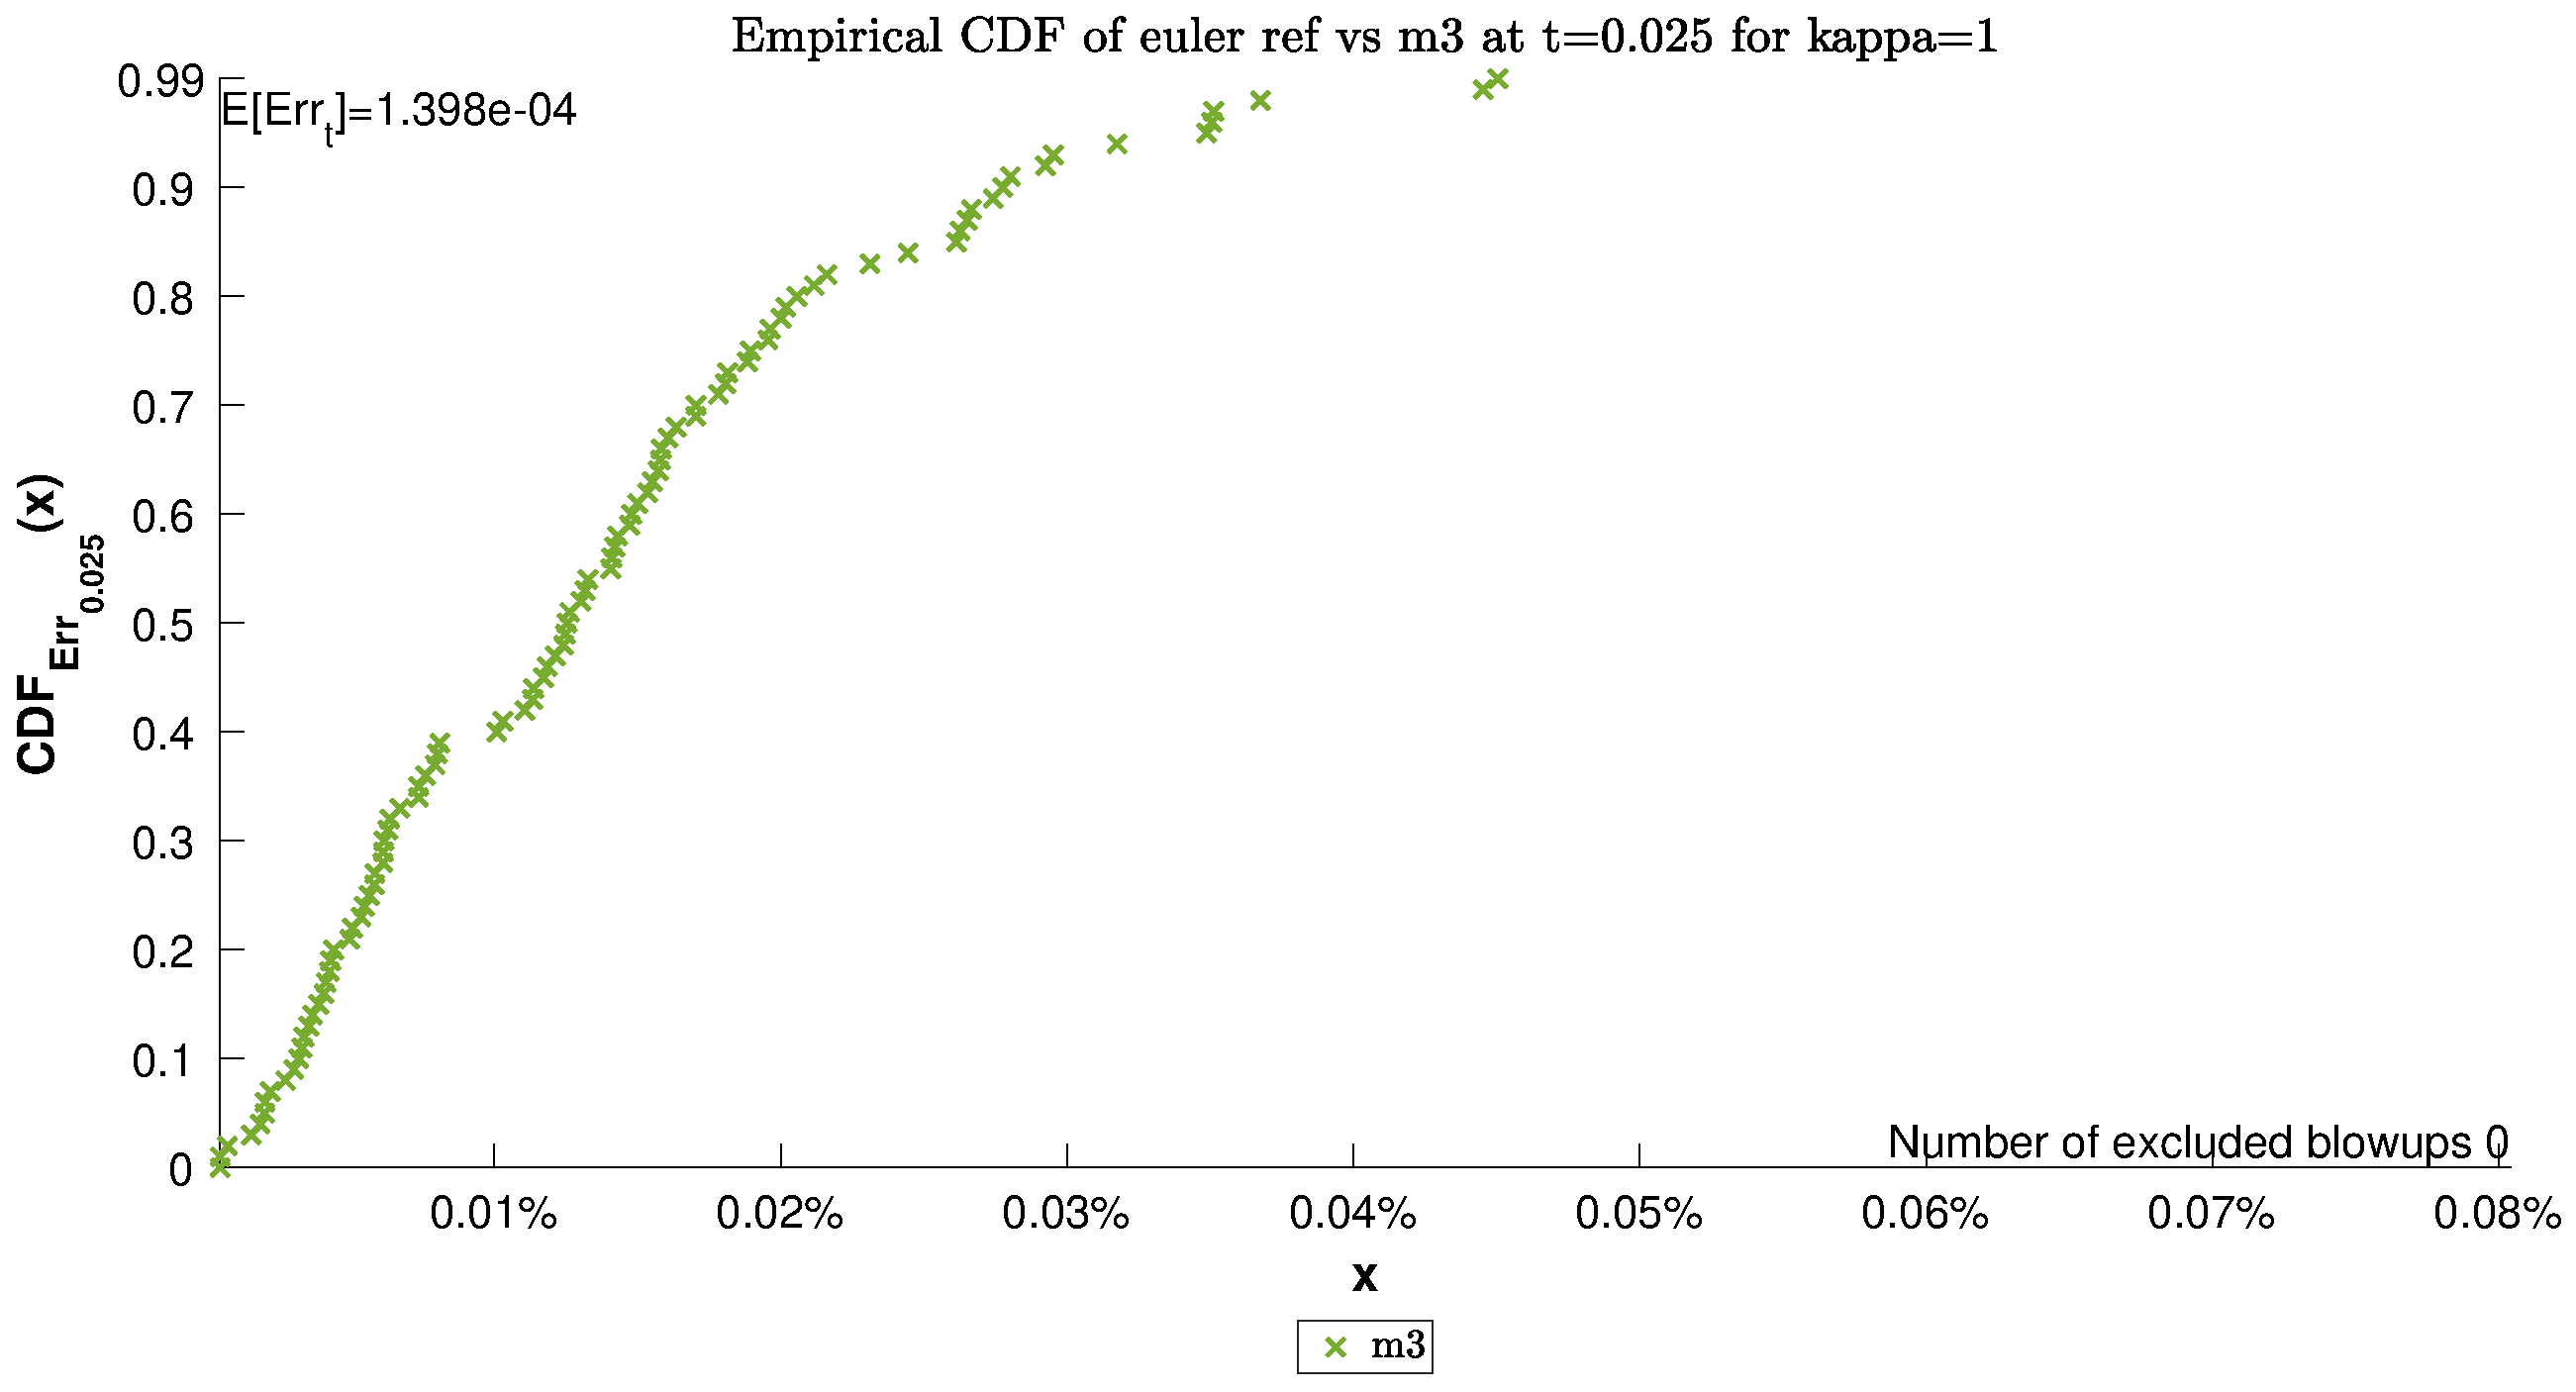
\includegraphics[width=.95\columnwidth]{CDF/CDFEulerRef_28}
\end{landscape}
\begin{landscape}
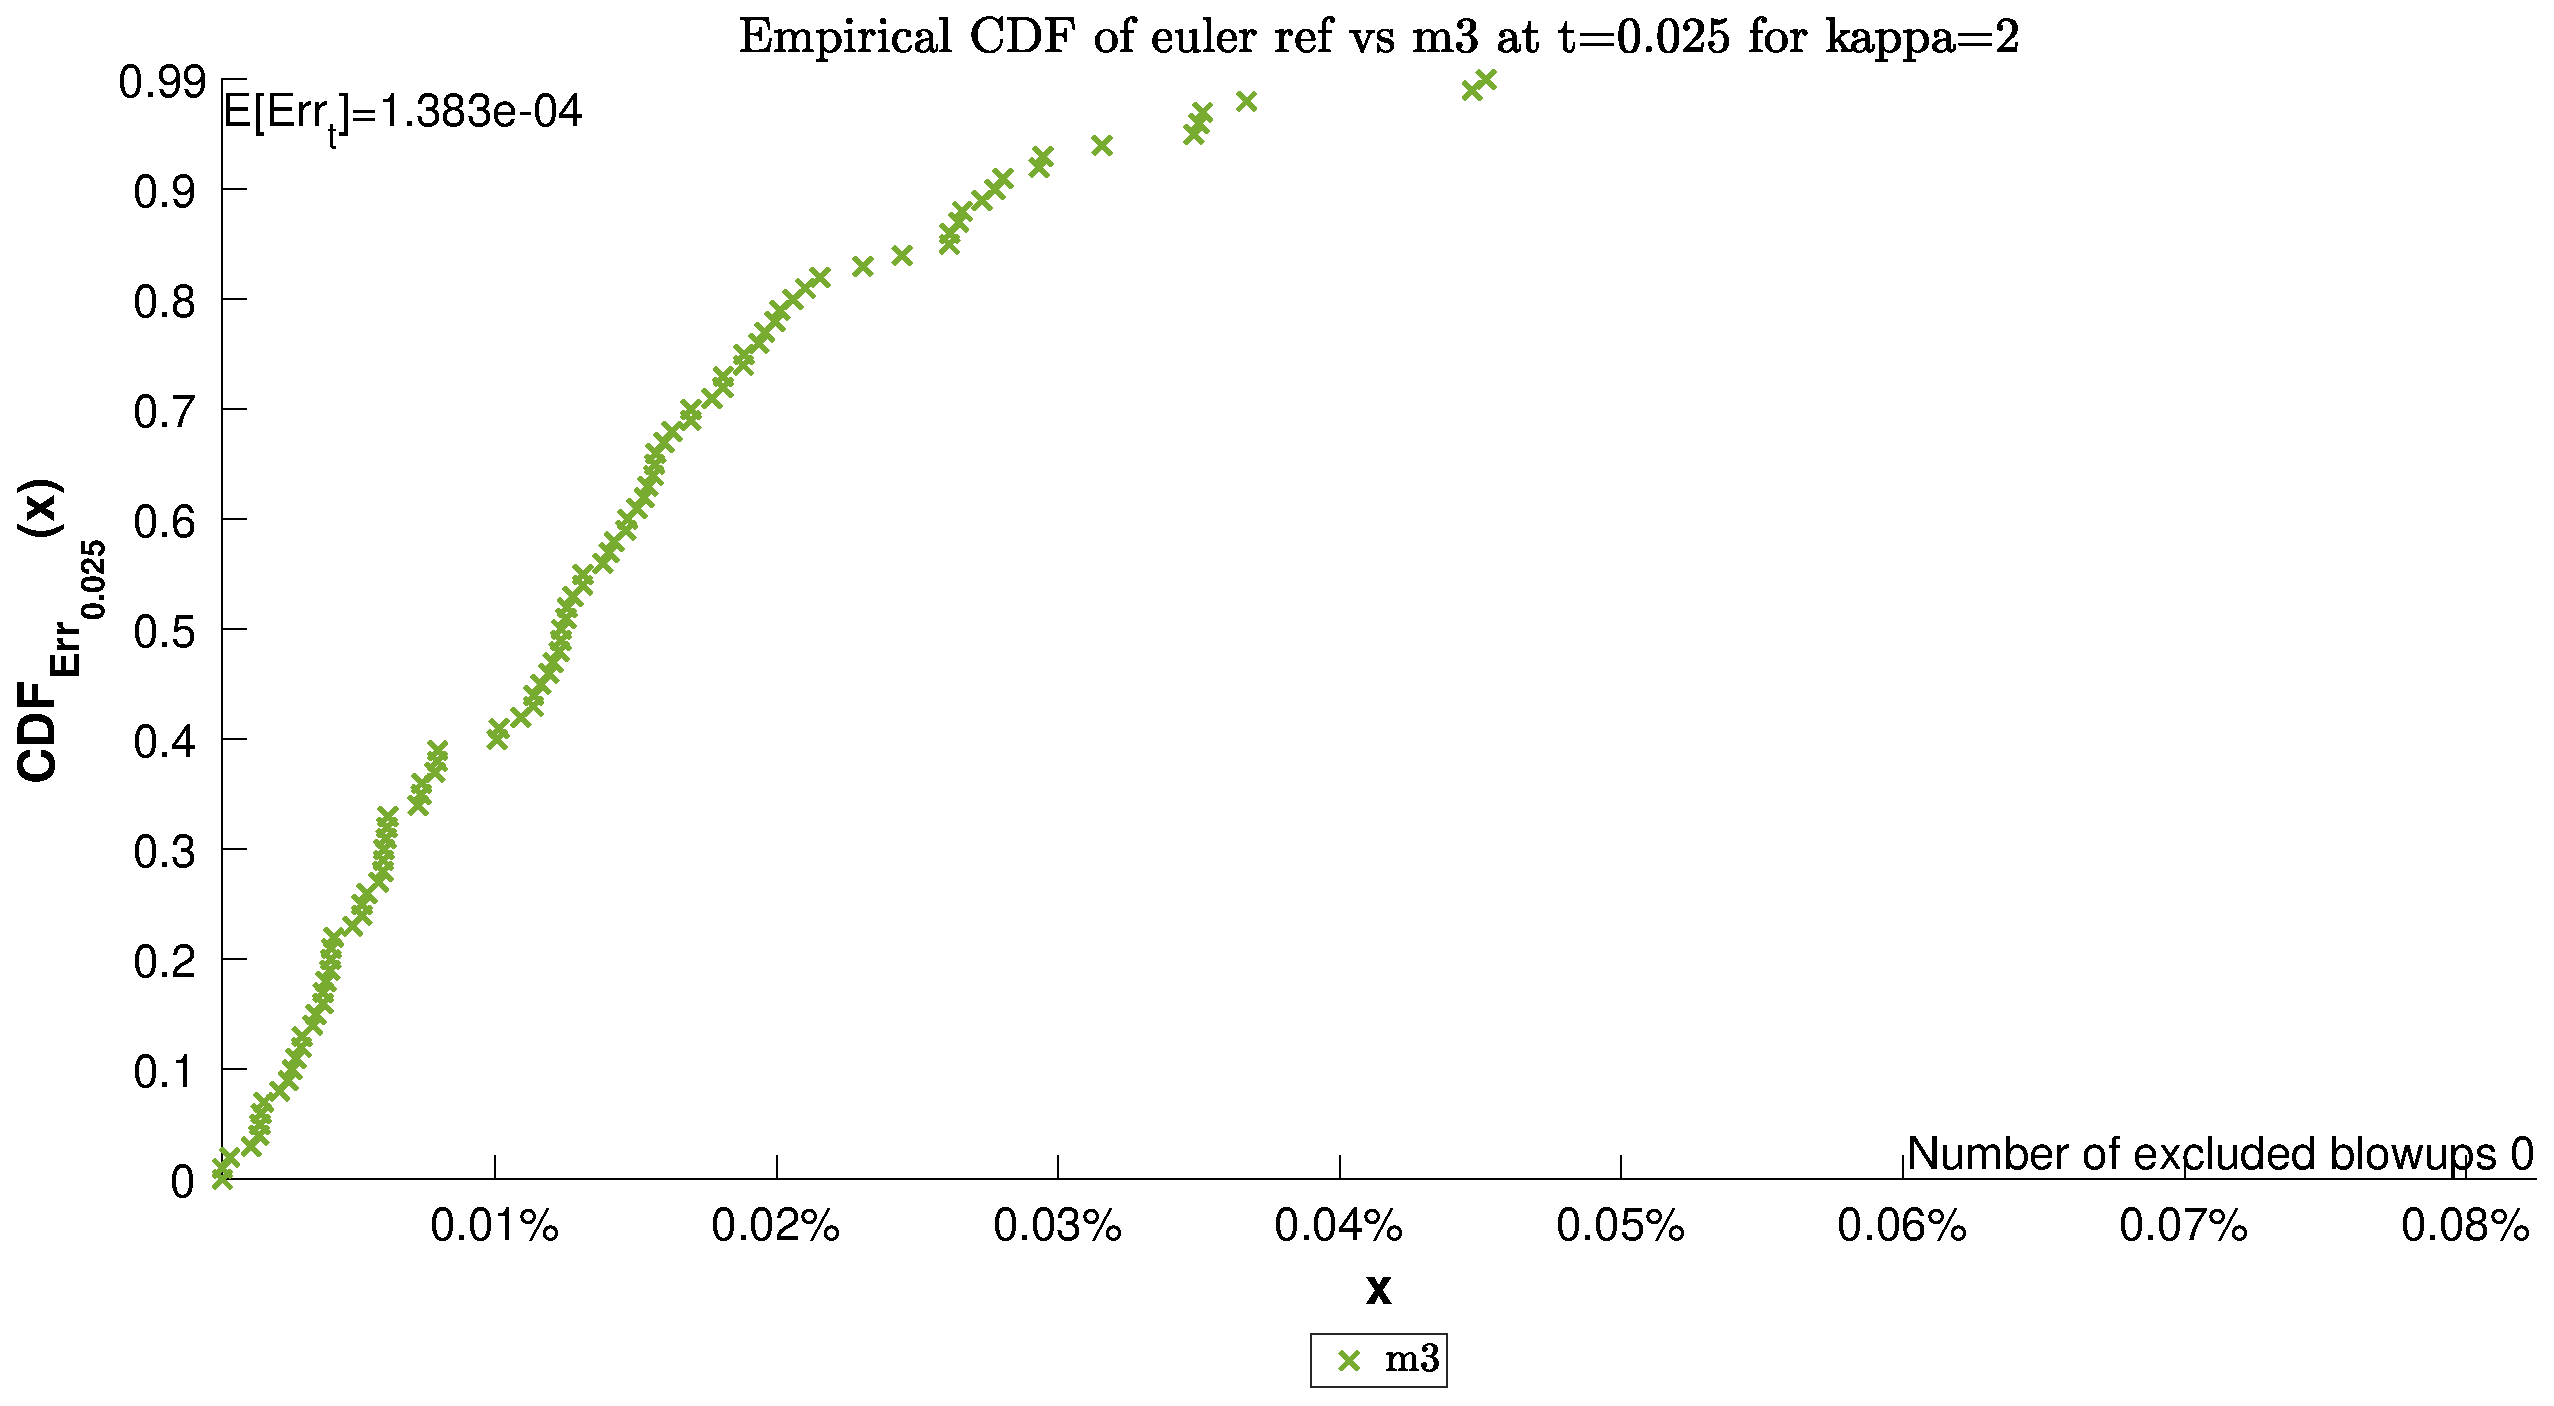
\includegraphics[width=.95\columnwidth]{CDF/CDFEulerRef_29}
\end{landscape}
\begin{landscape}
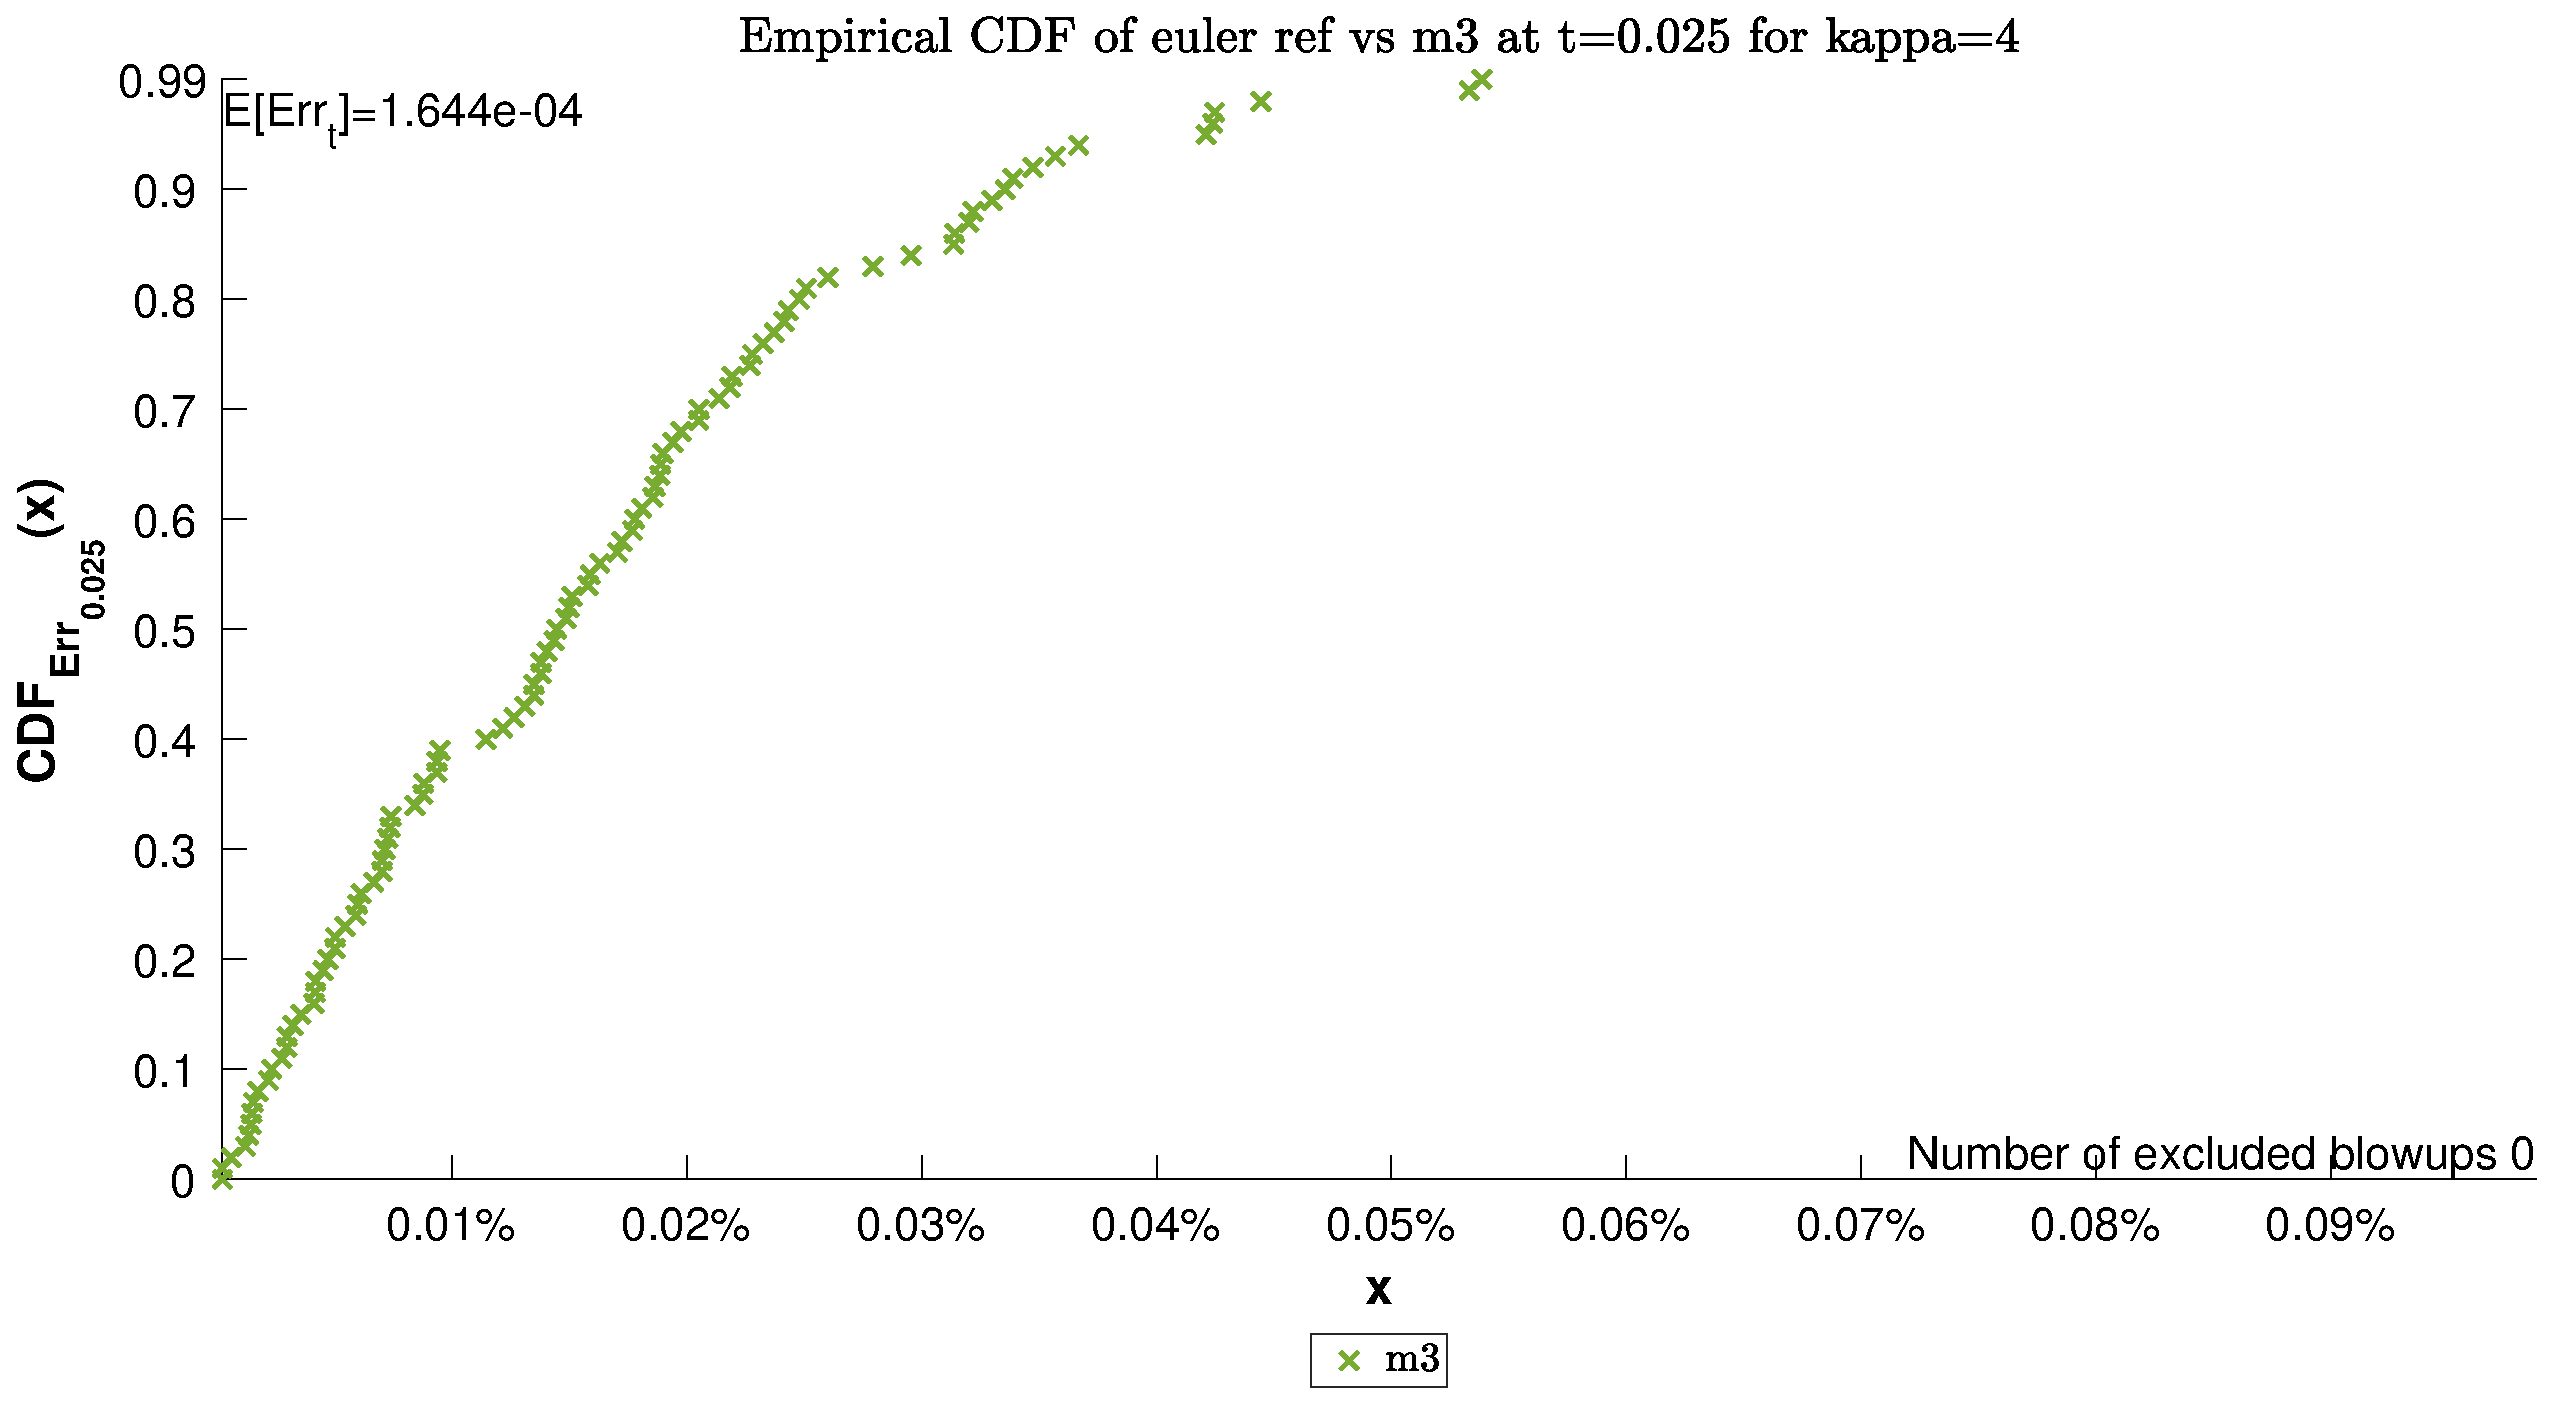
\includegraphics[width=.95\columnwidth]{CDF/CDFEulerRef_30}
\end{landscape}
\begin{landscape}
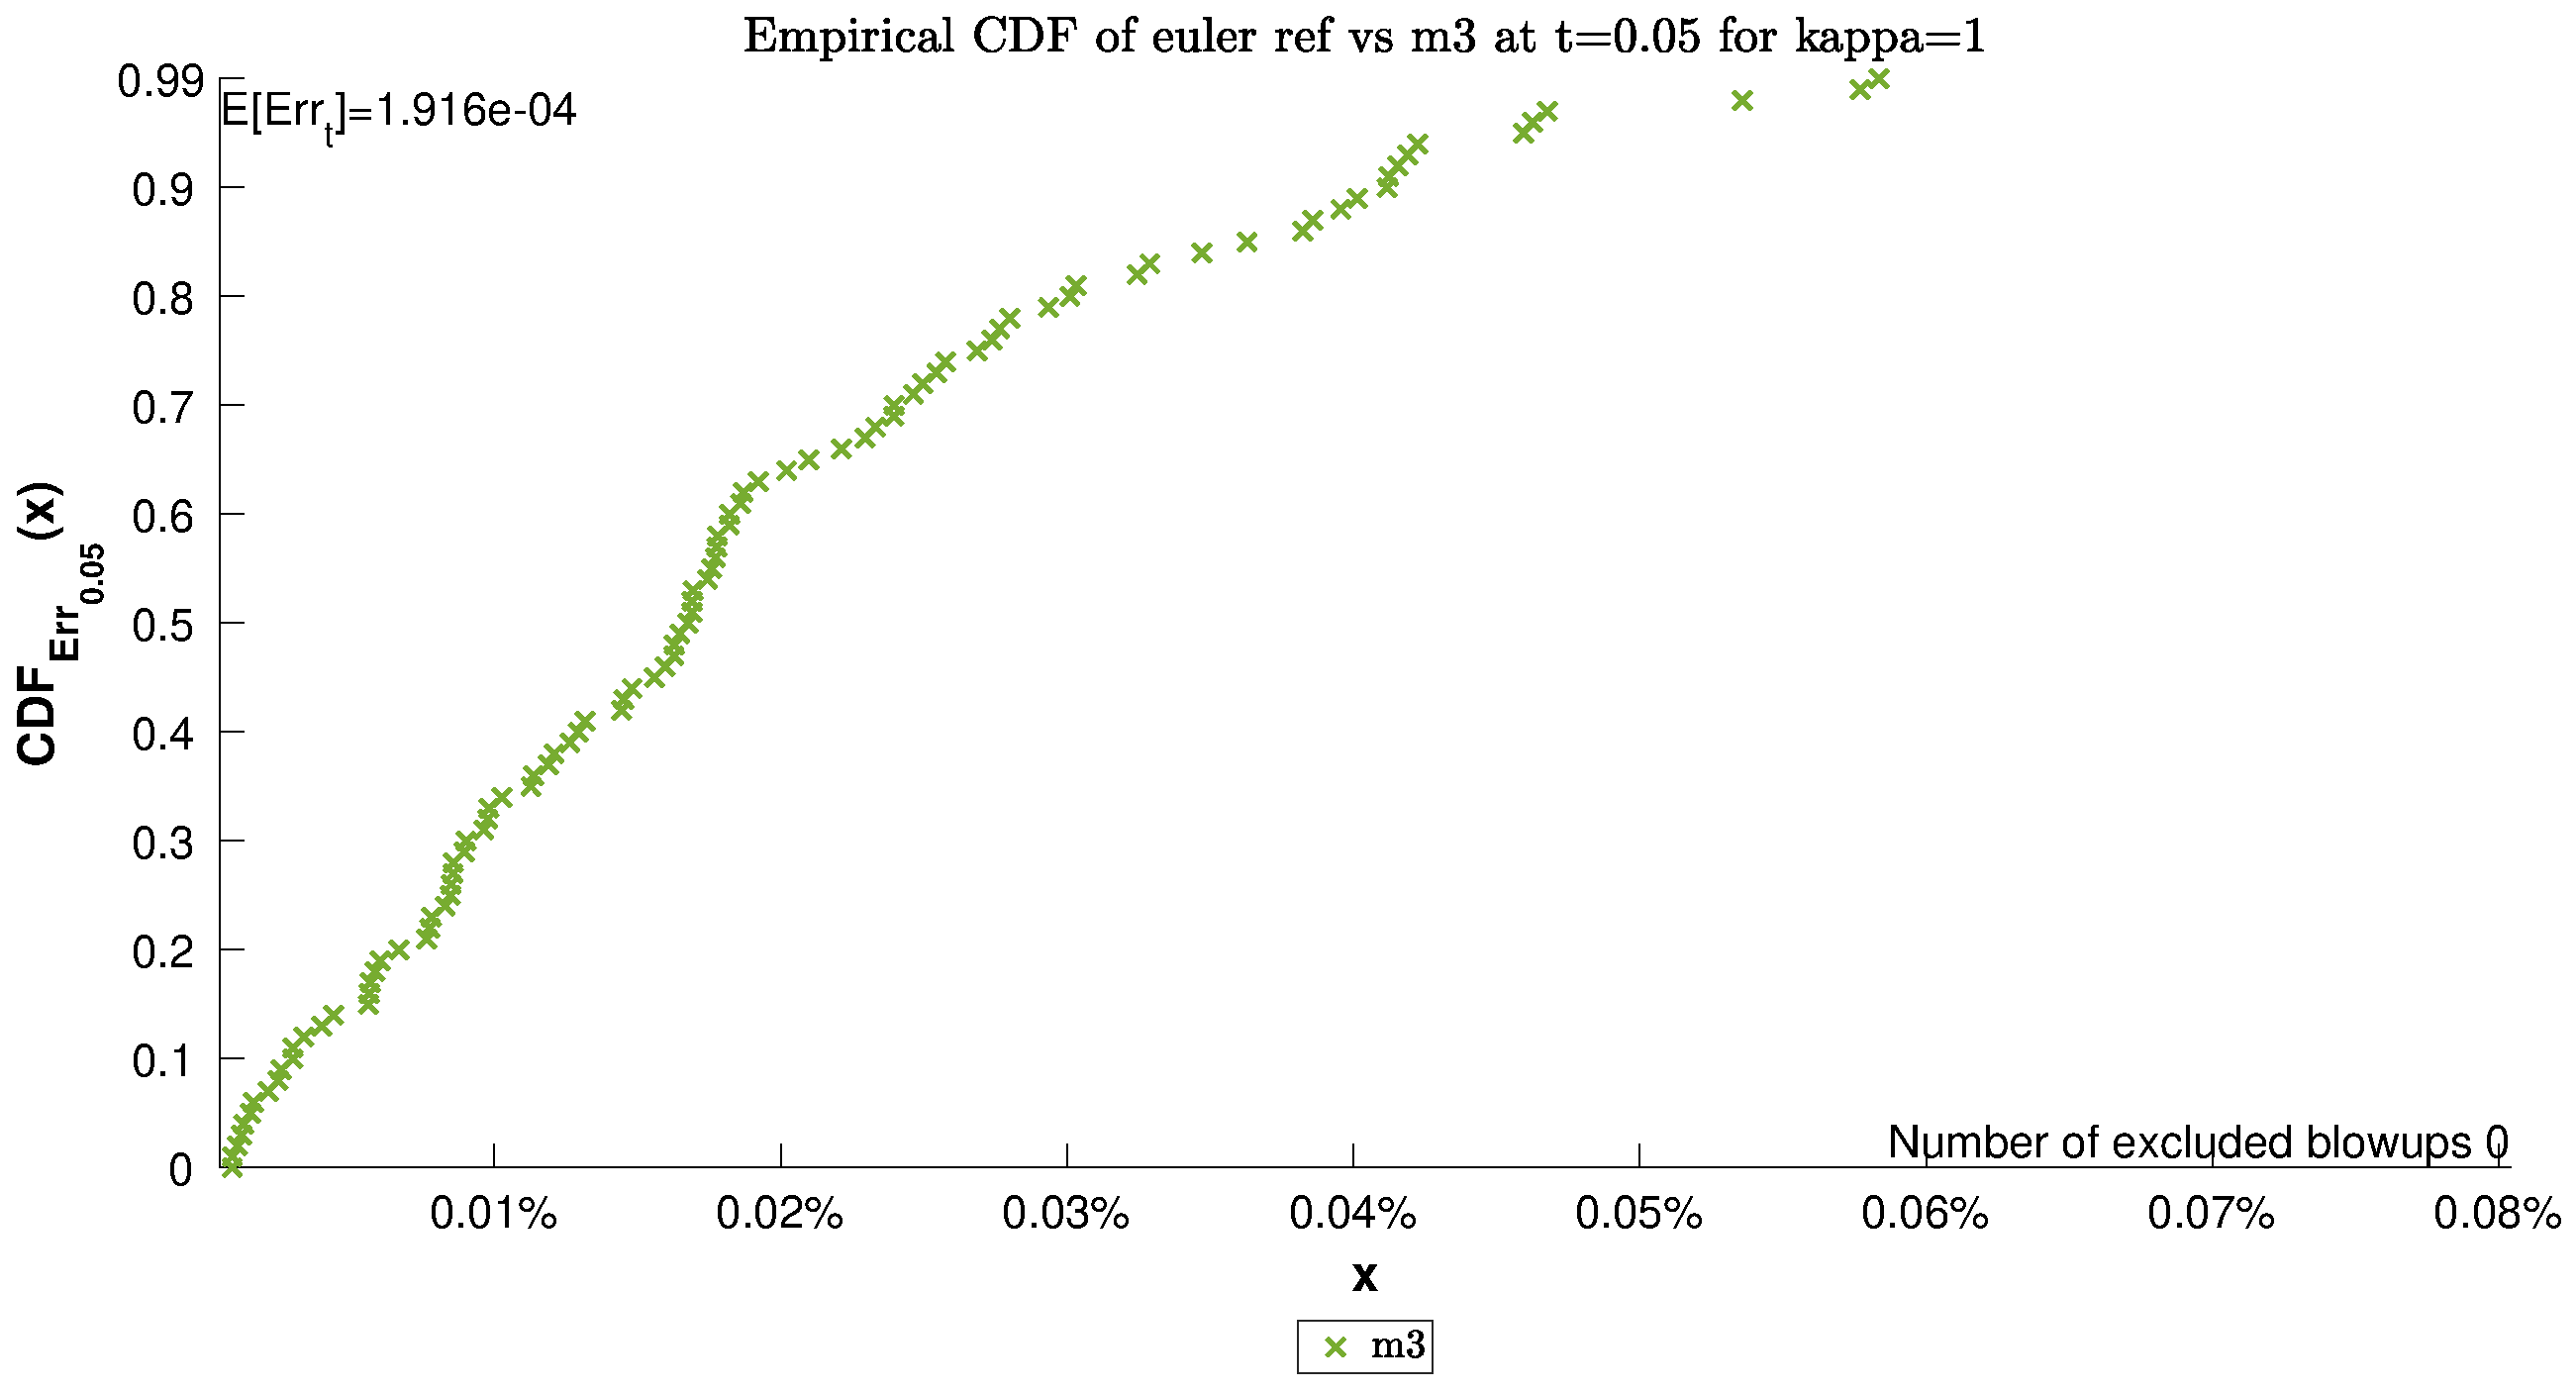
\includegraphics[width=.95\columnwidth]{CDF/CDFEulerRef_31}
\end{landscape}
\begin{landscape}
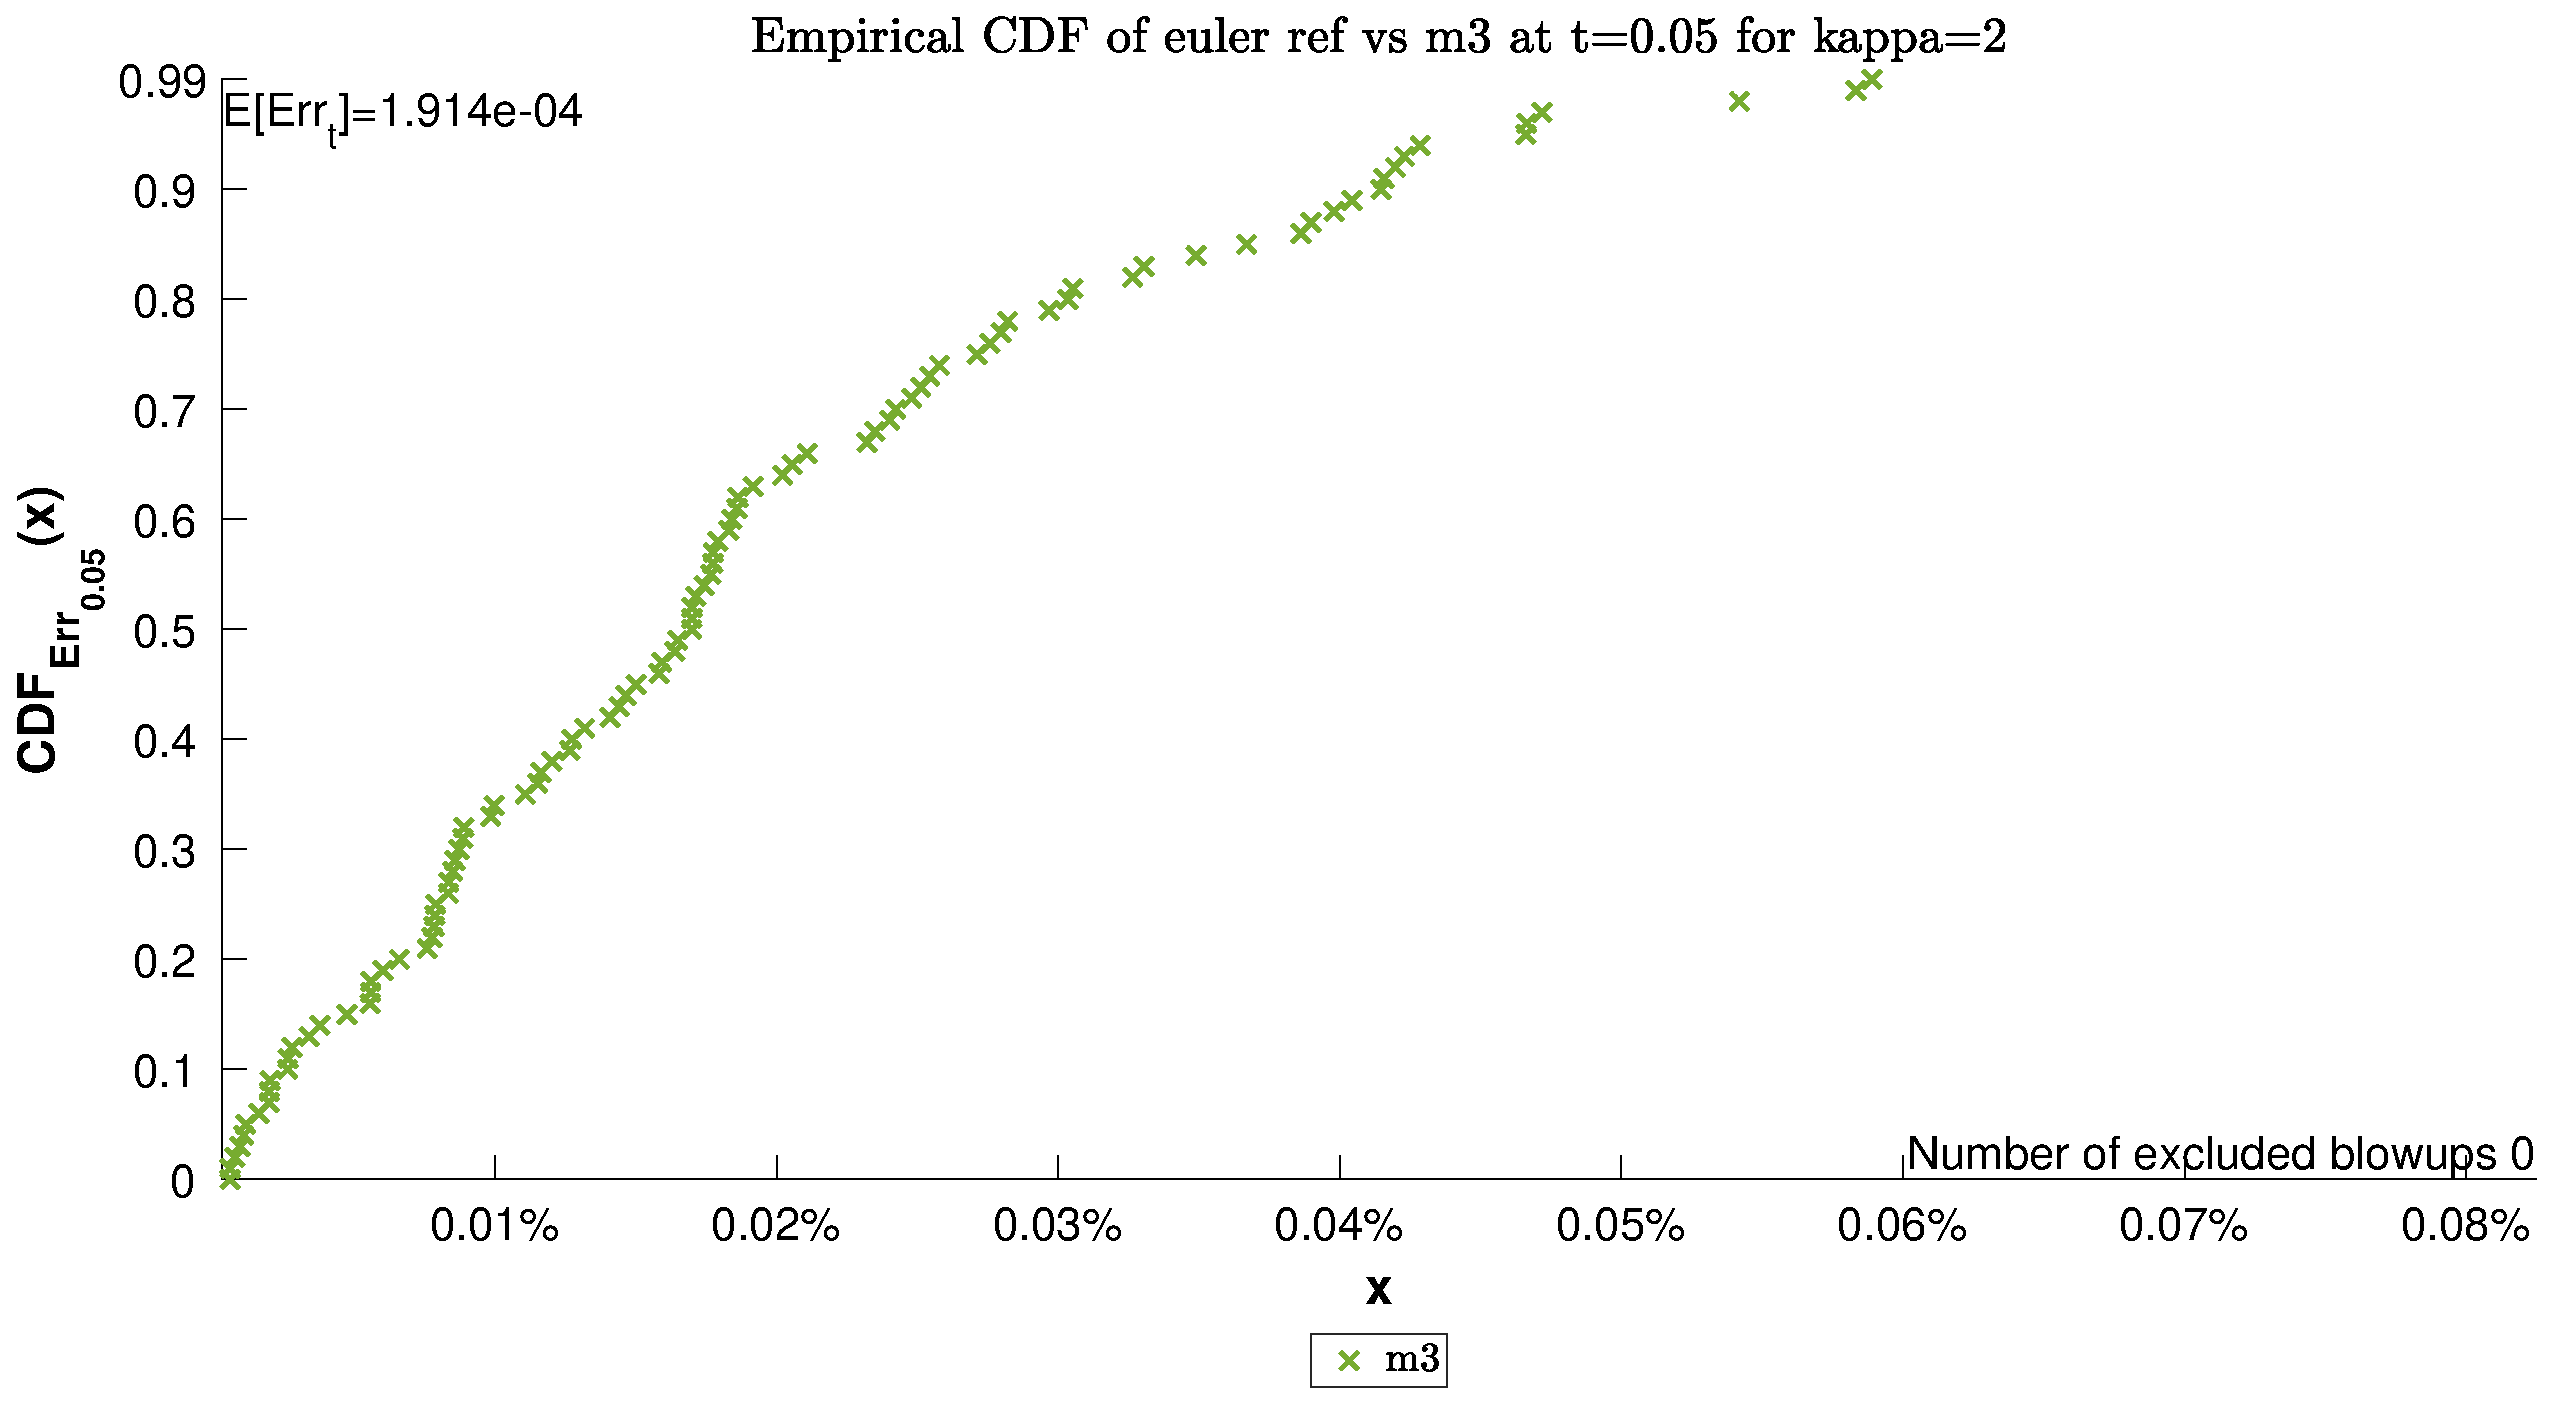
\includegraphics[width=.95\columnwidth]{CDF/CDFEulerRef_32}
\end{landscape}
\begin{landscape}
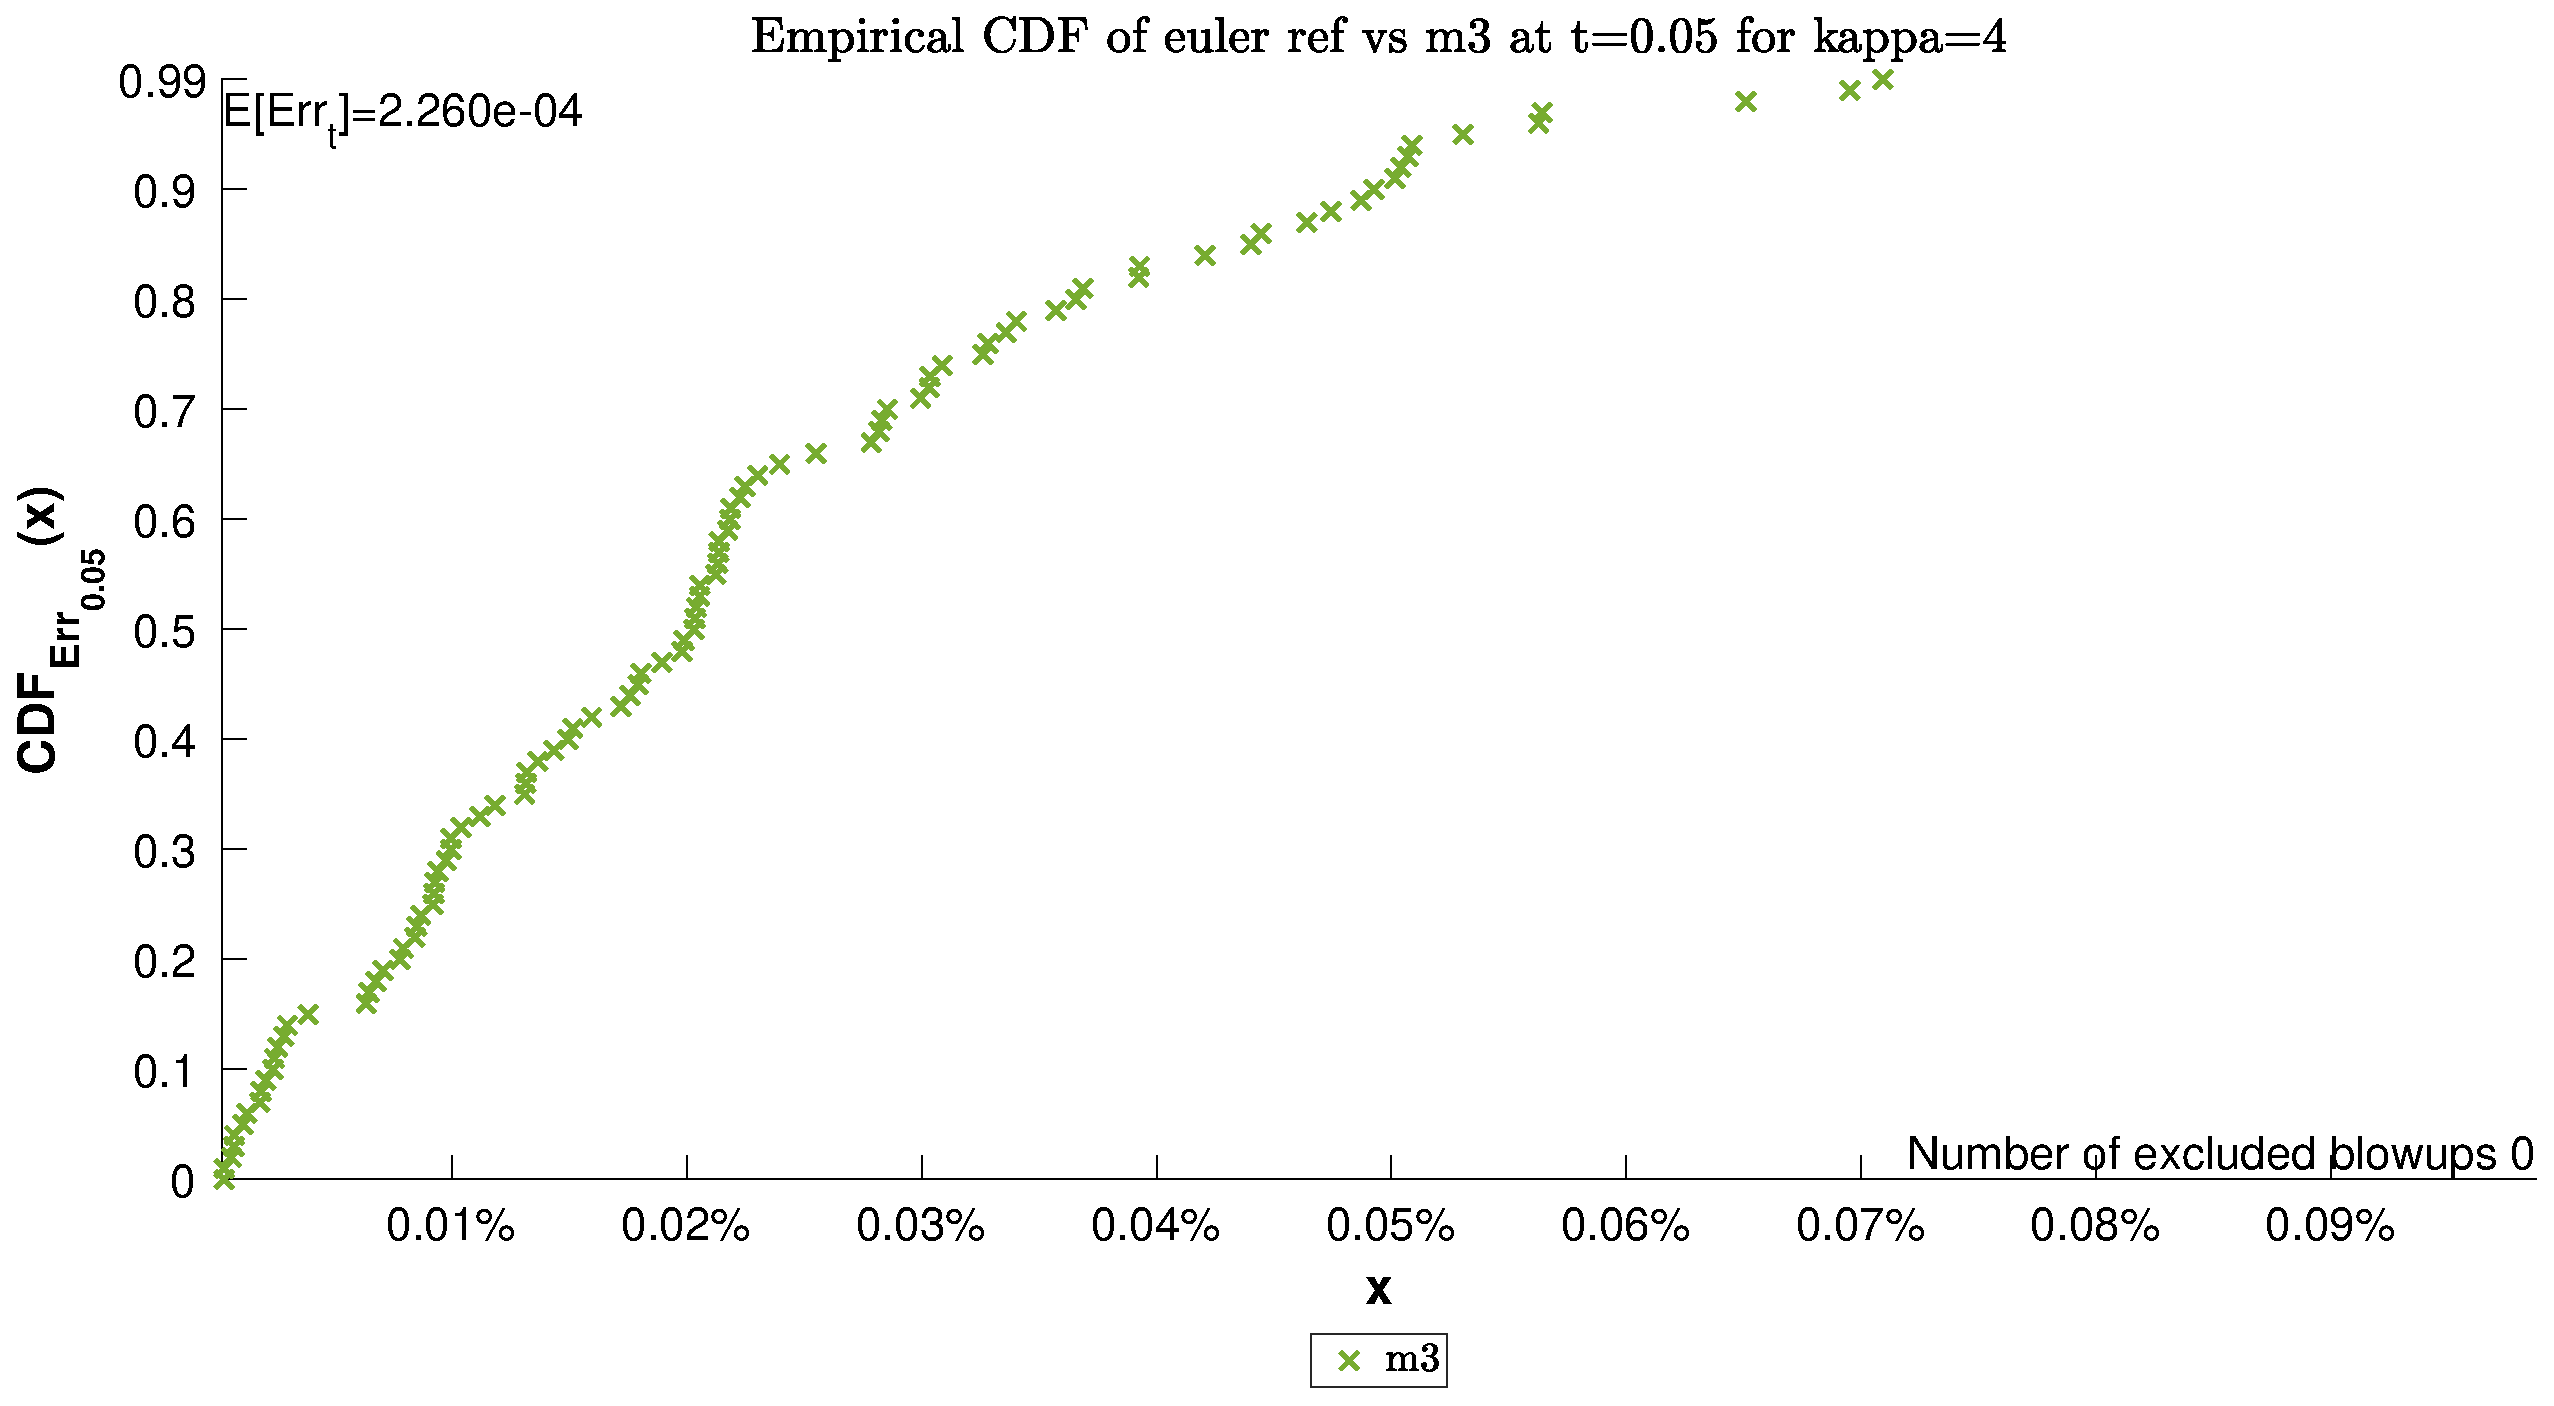
\includegraphics[width=.95\columnwidth]{CDF/CDFEulerRef_33}
\end{landscape}
\begin{landscape}
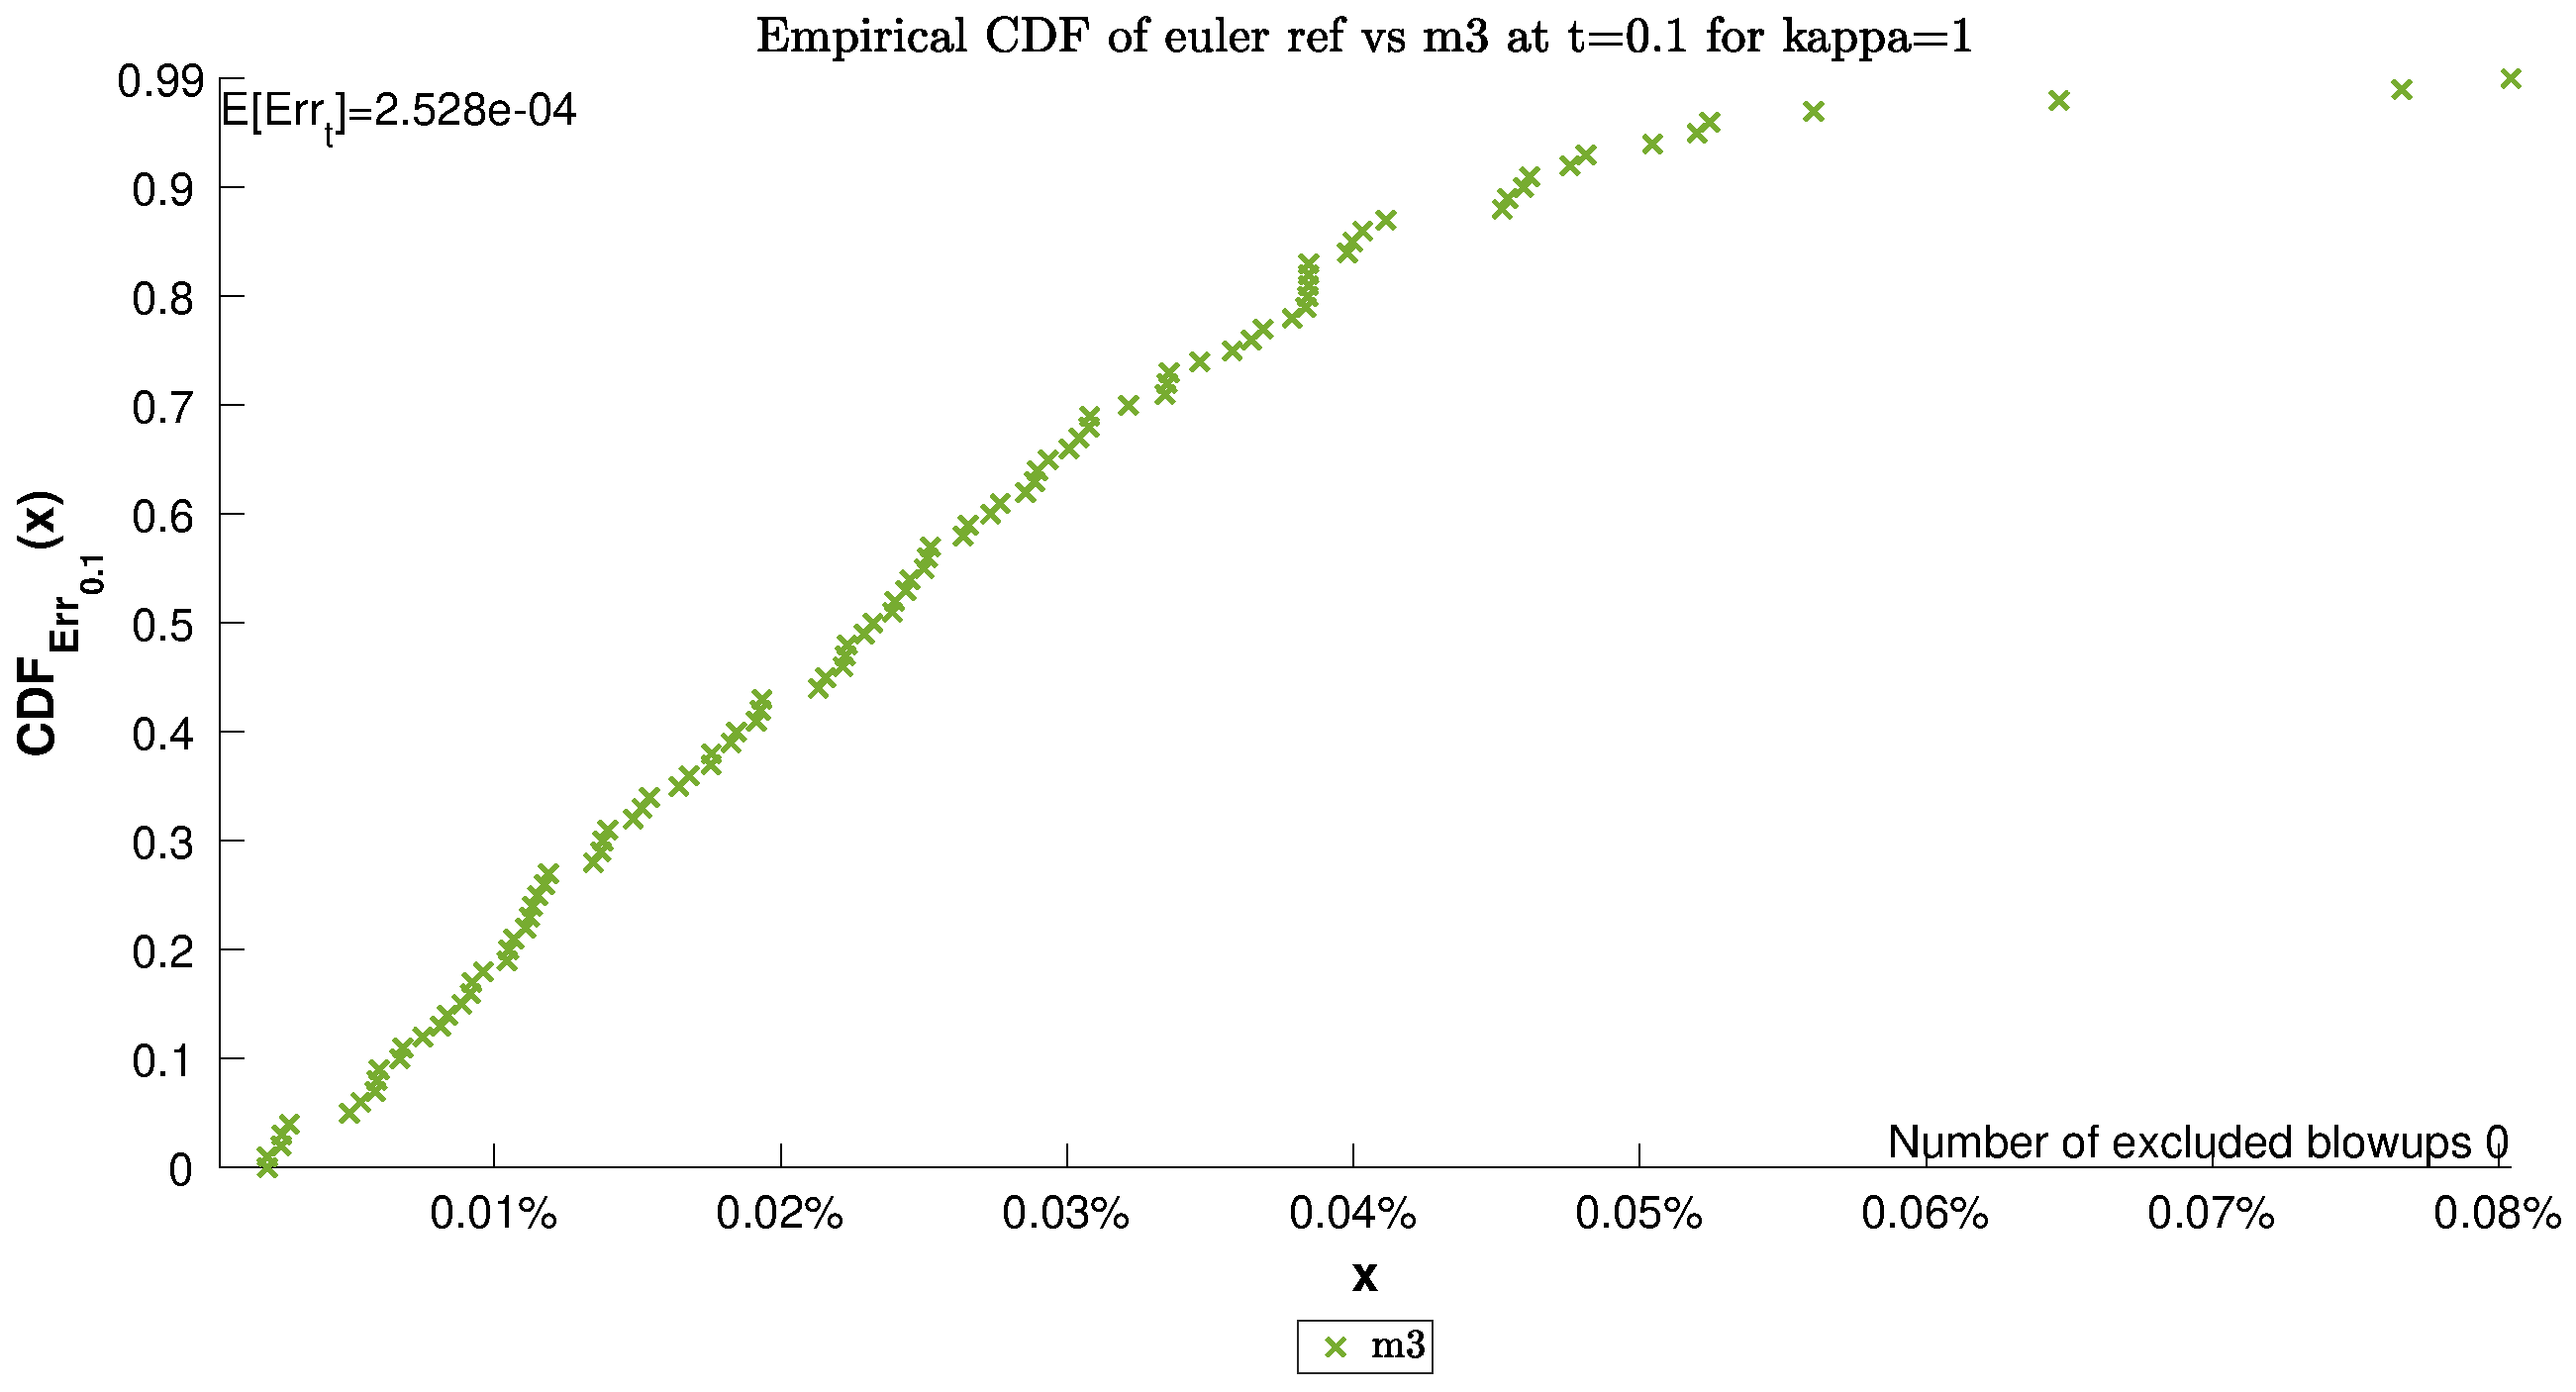
\includegraphics[width=.95\columnwidth]{CDF/CDFEulerRef_34}
\end{landscape}
\begin{landscape}
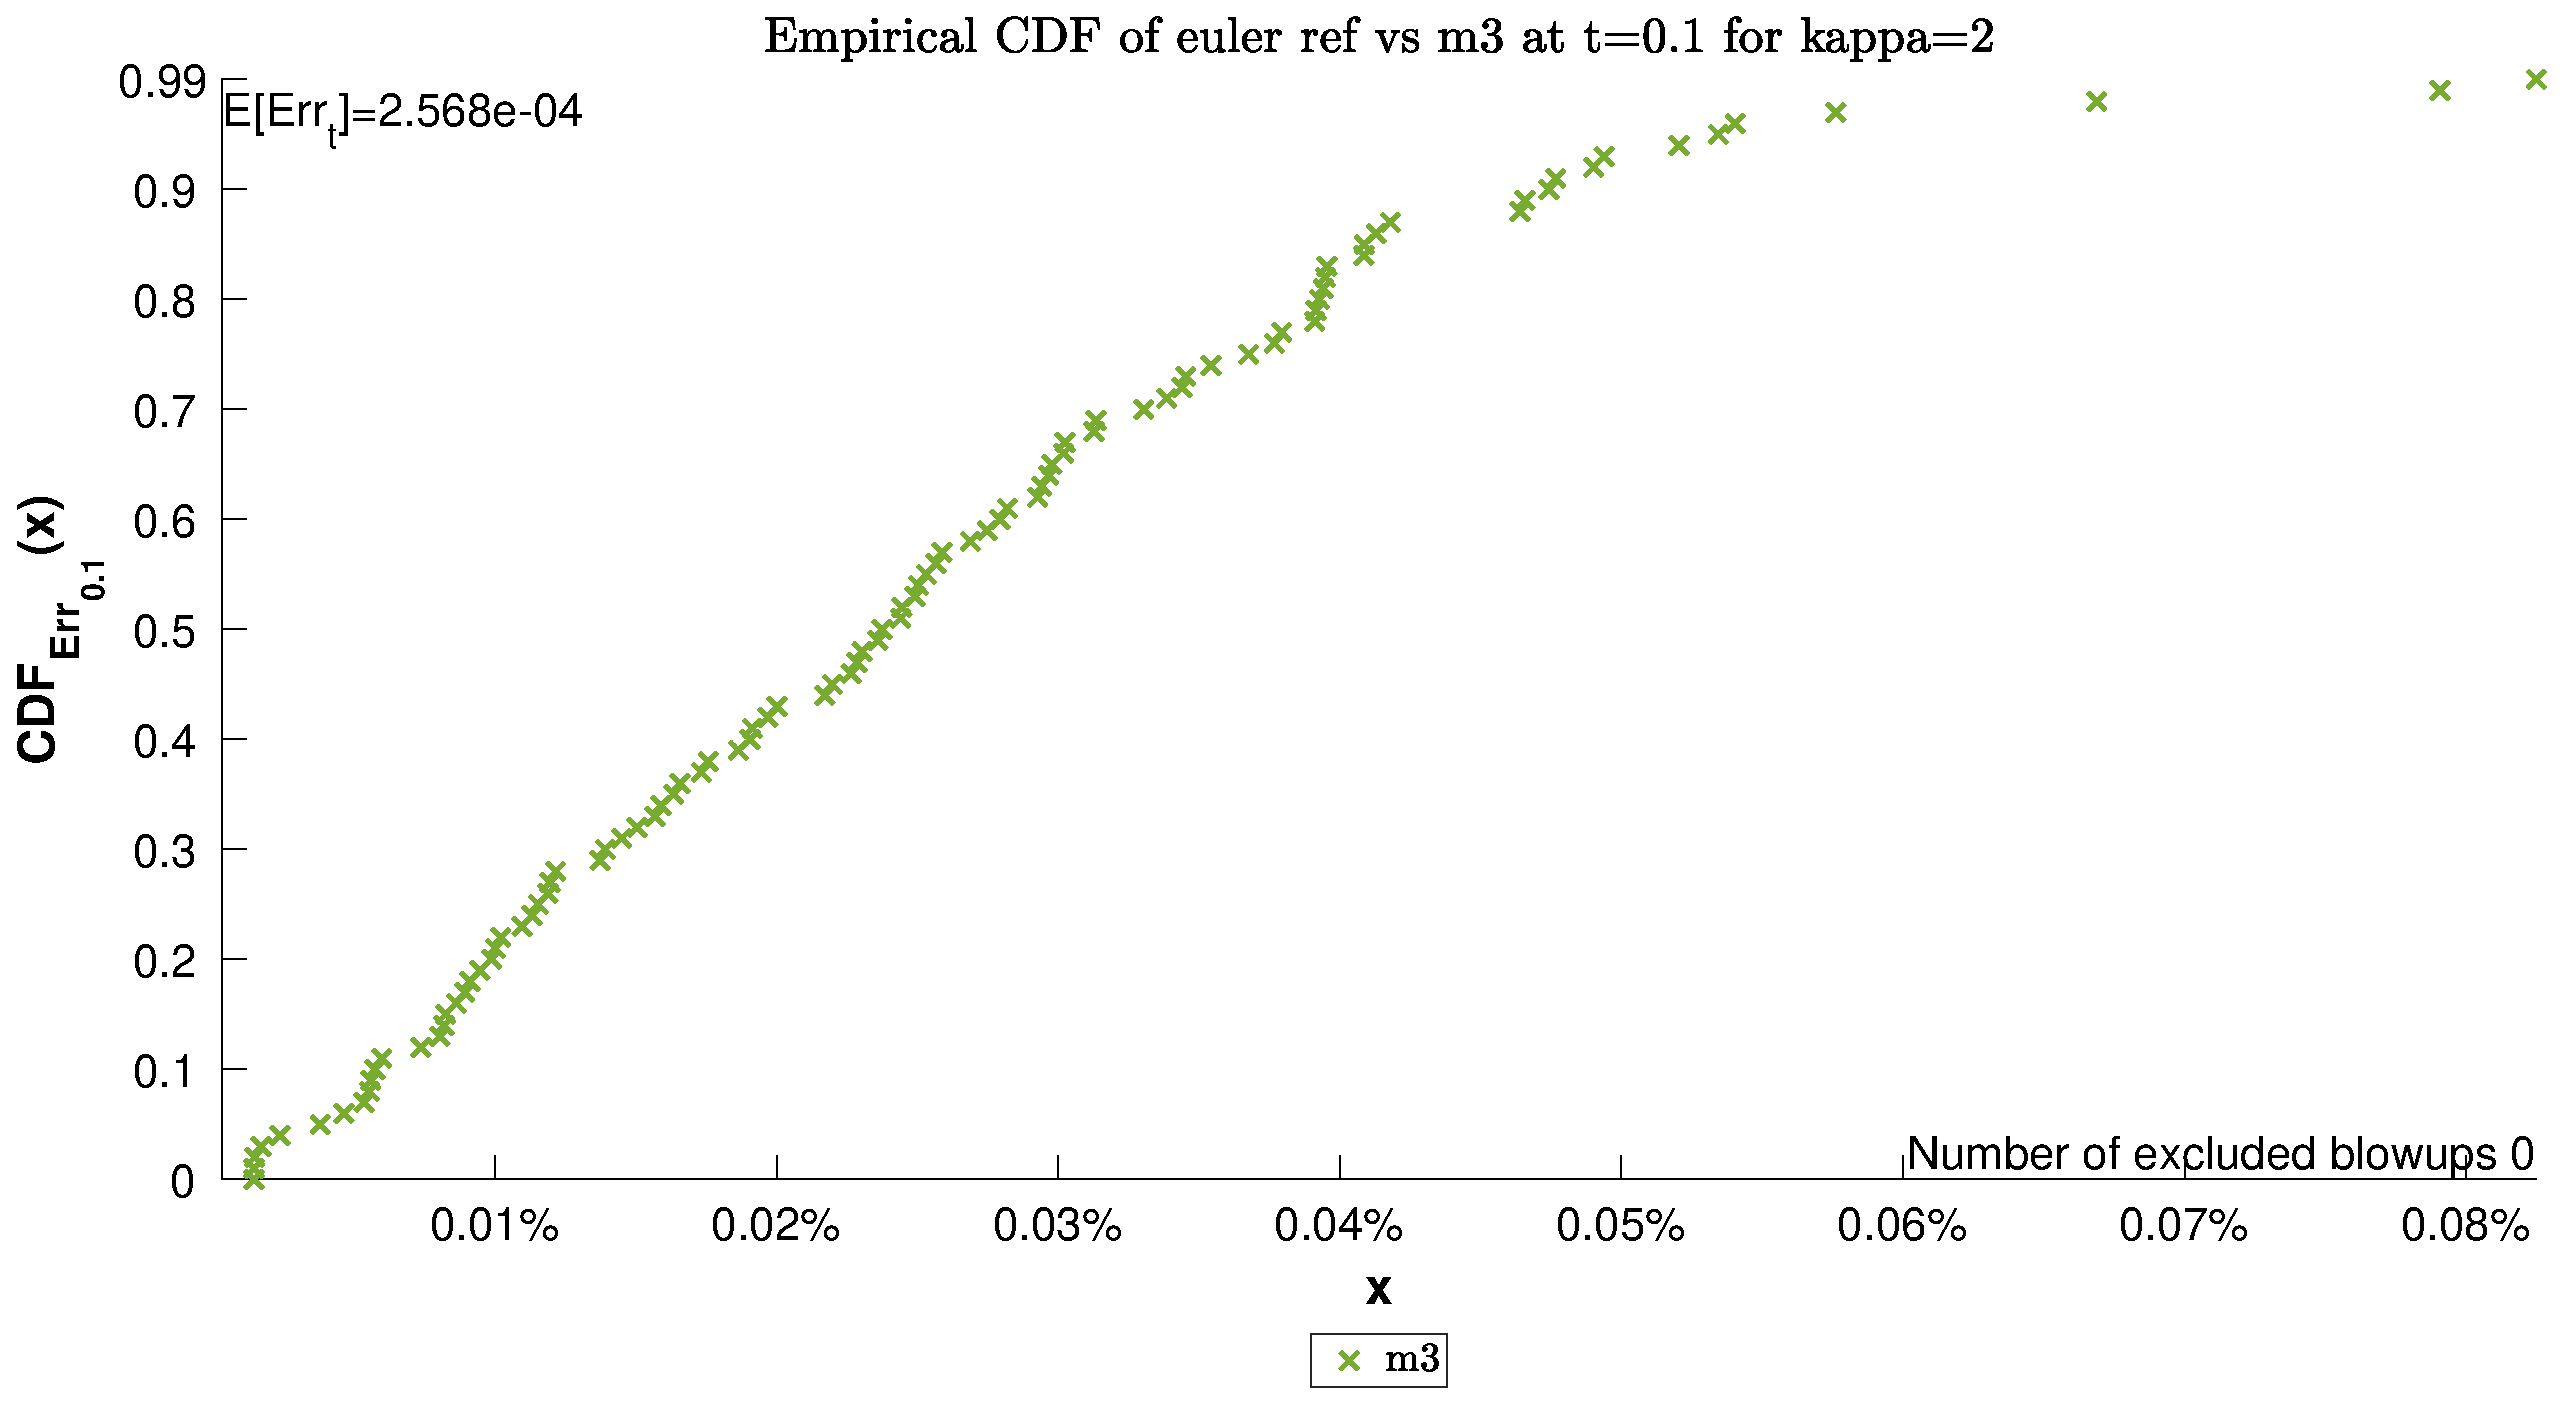
\includegraphics[width=.95\columnwidth]{CDF/CDFEulerRef_35}
\end{landscape}
\begin{landscape}
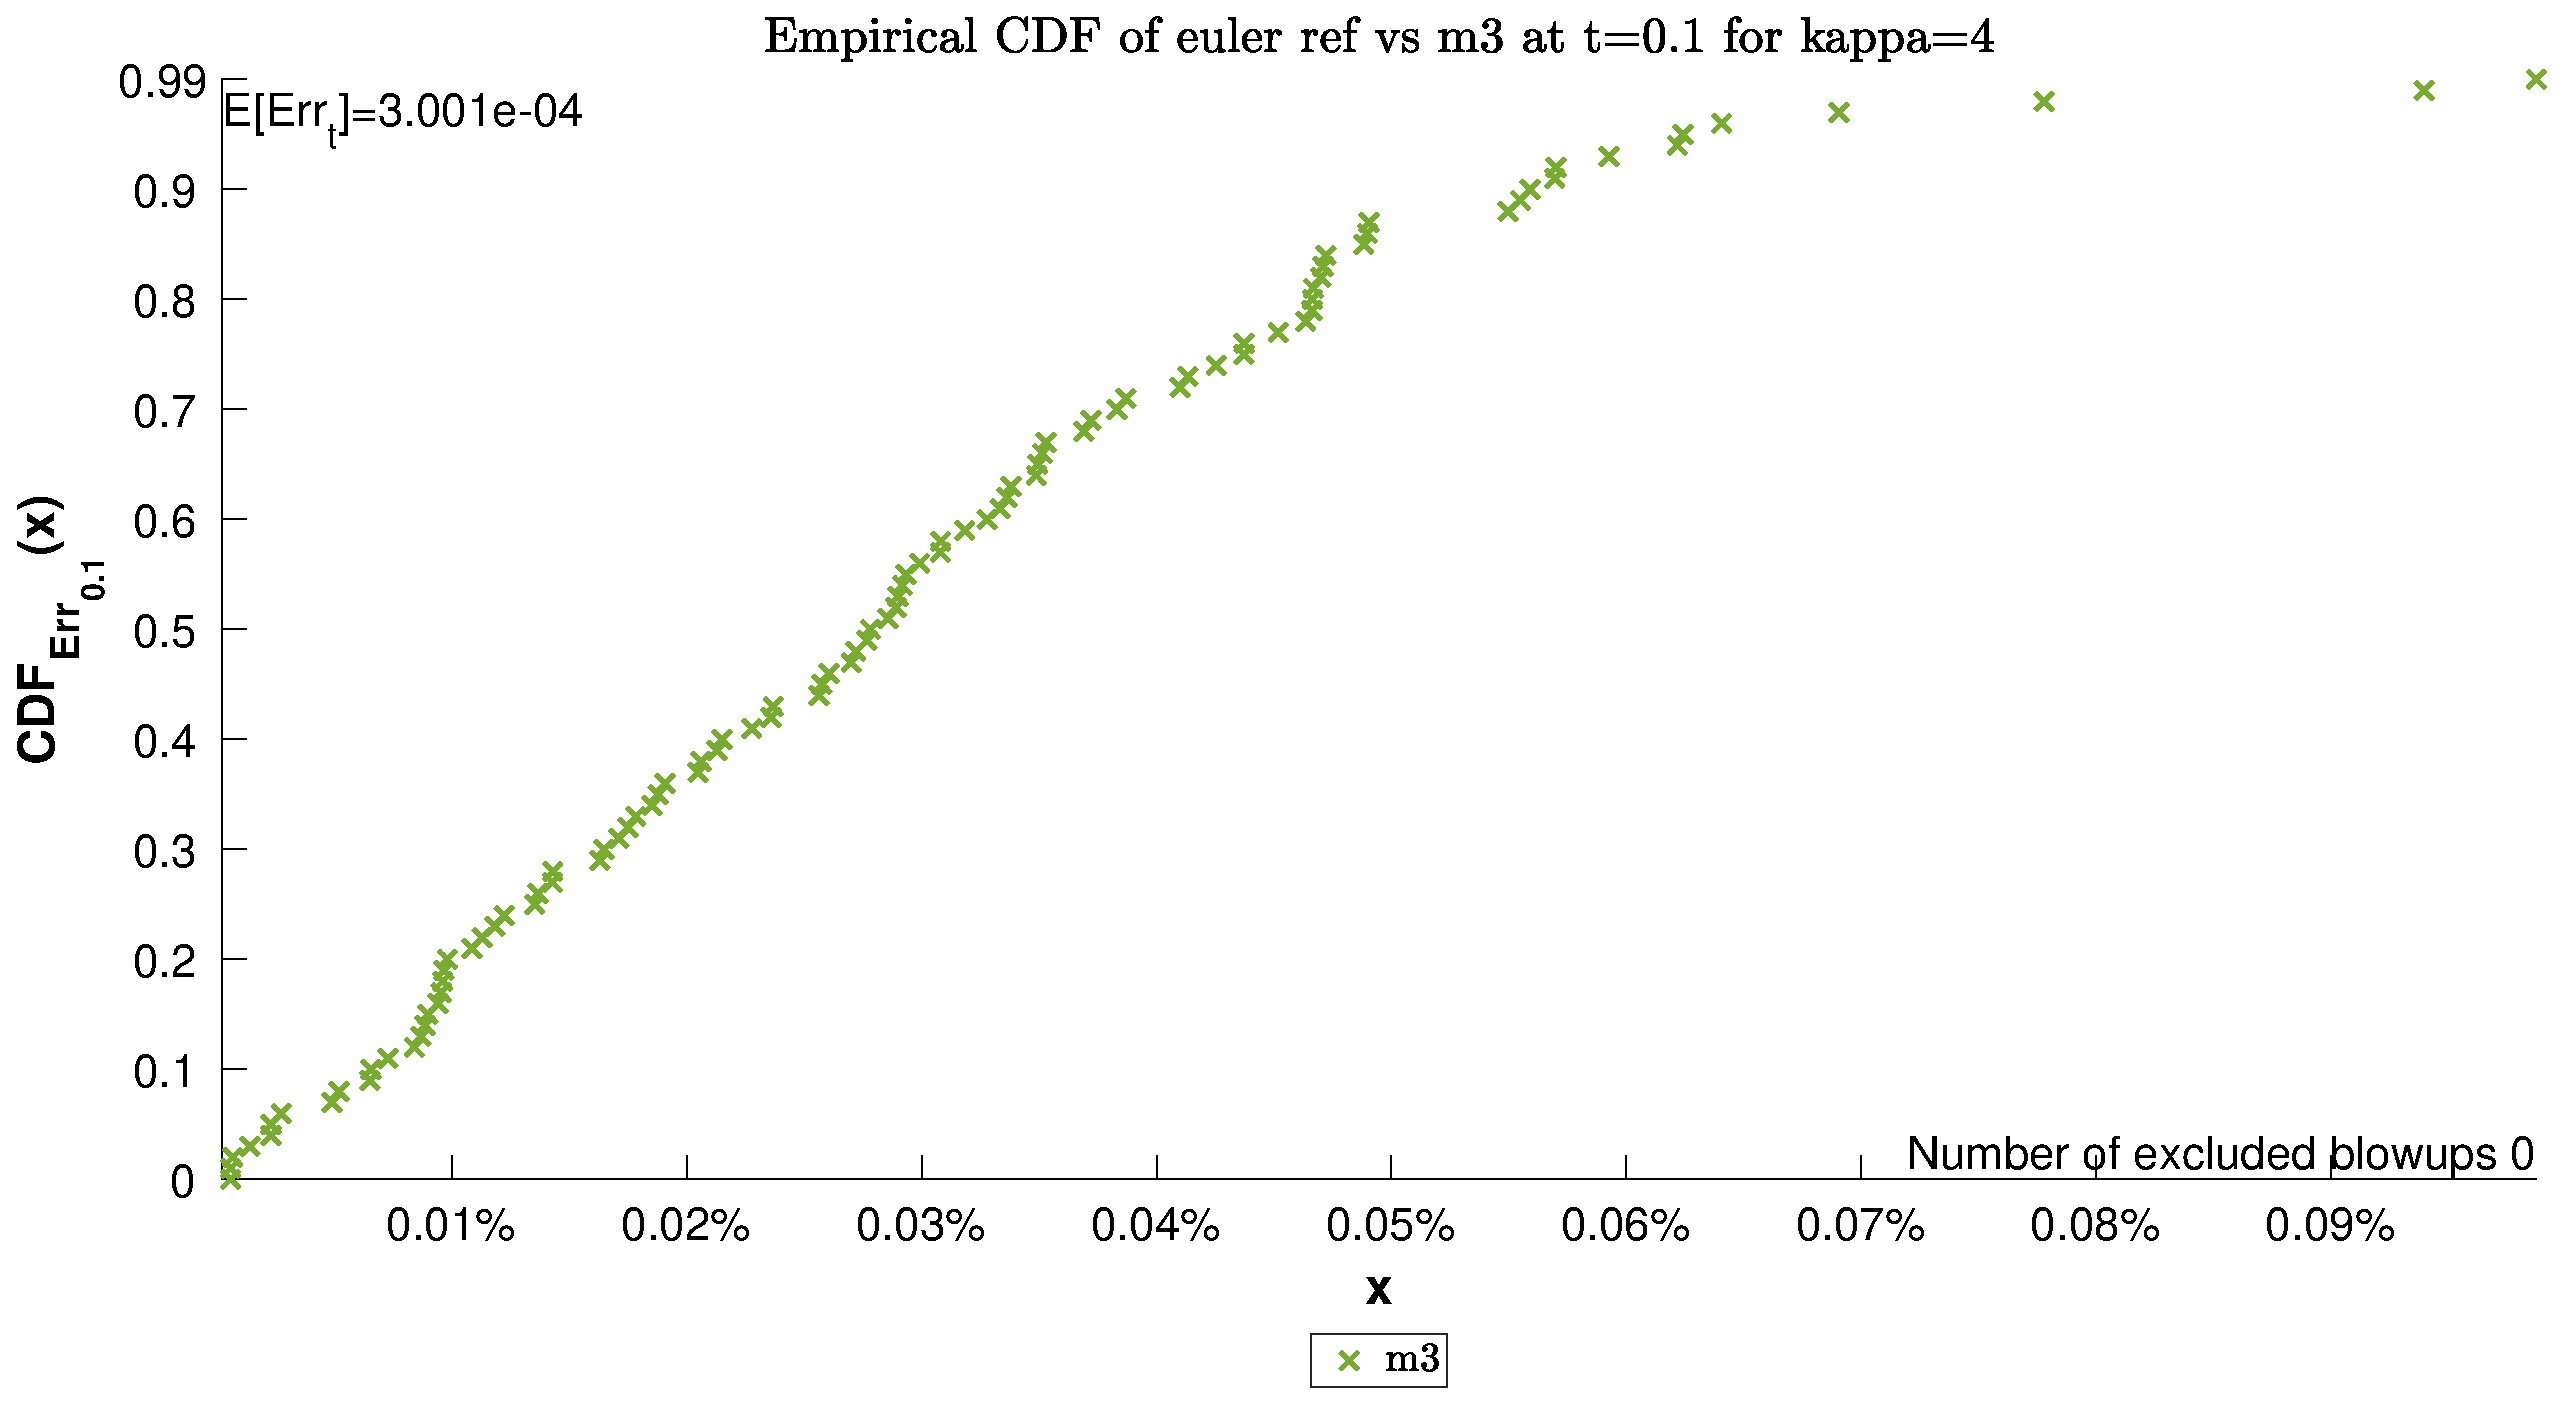
\includegraphics[width=.95\columnwidth]{CDF/CDFEulerRef_36}
\end{landscape}

\subsection{Sparsity Patterns}
	\begin{landscape}
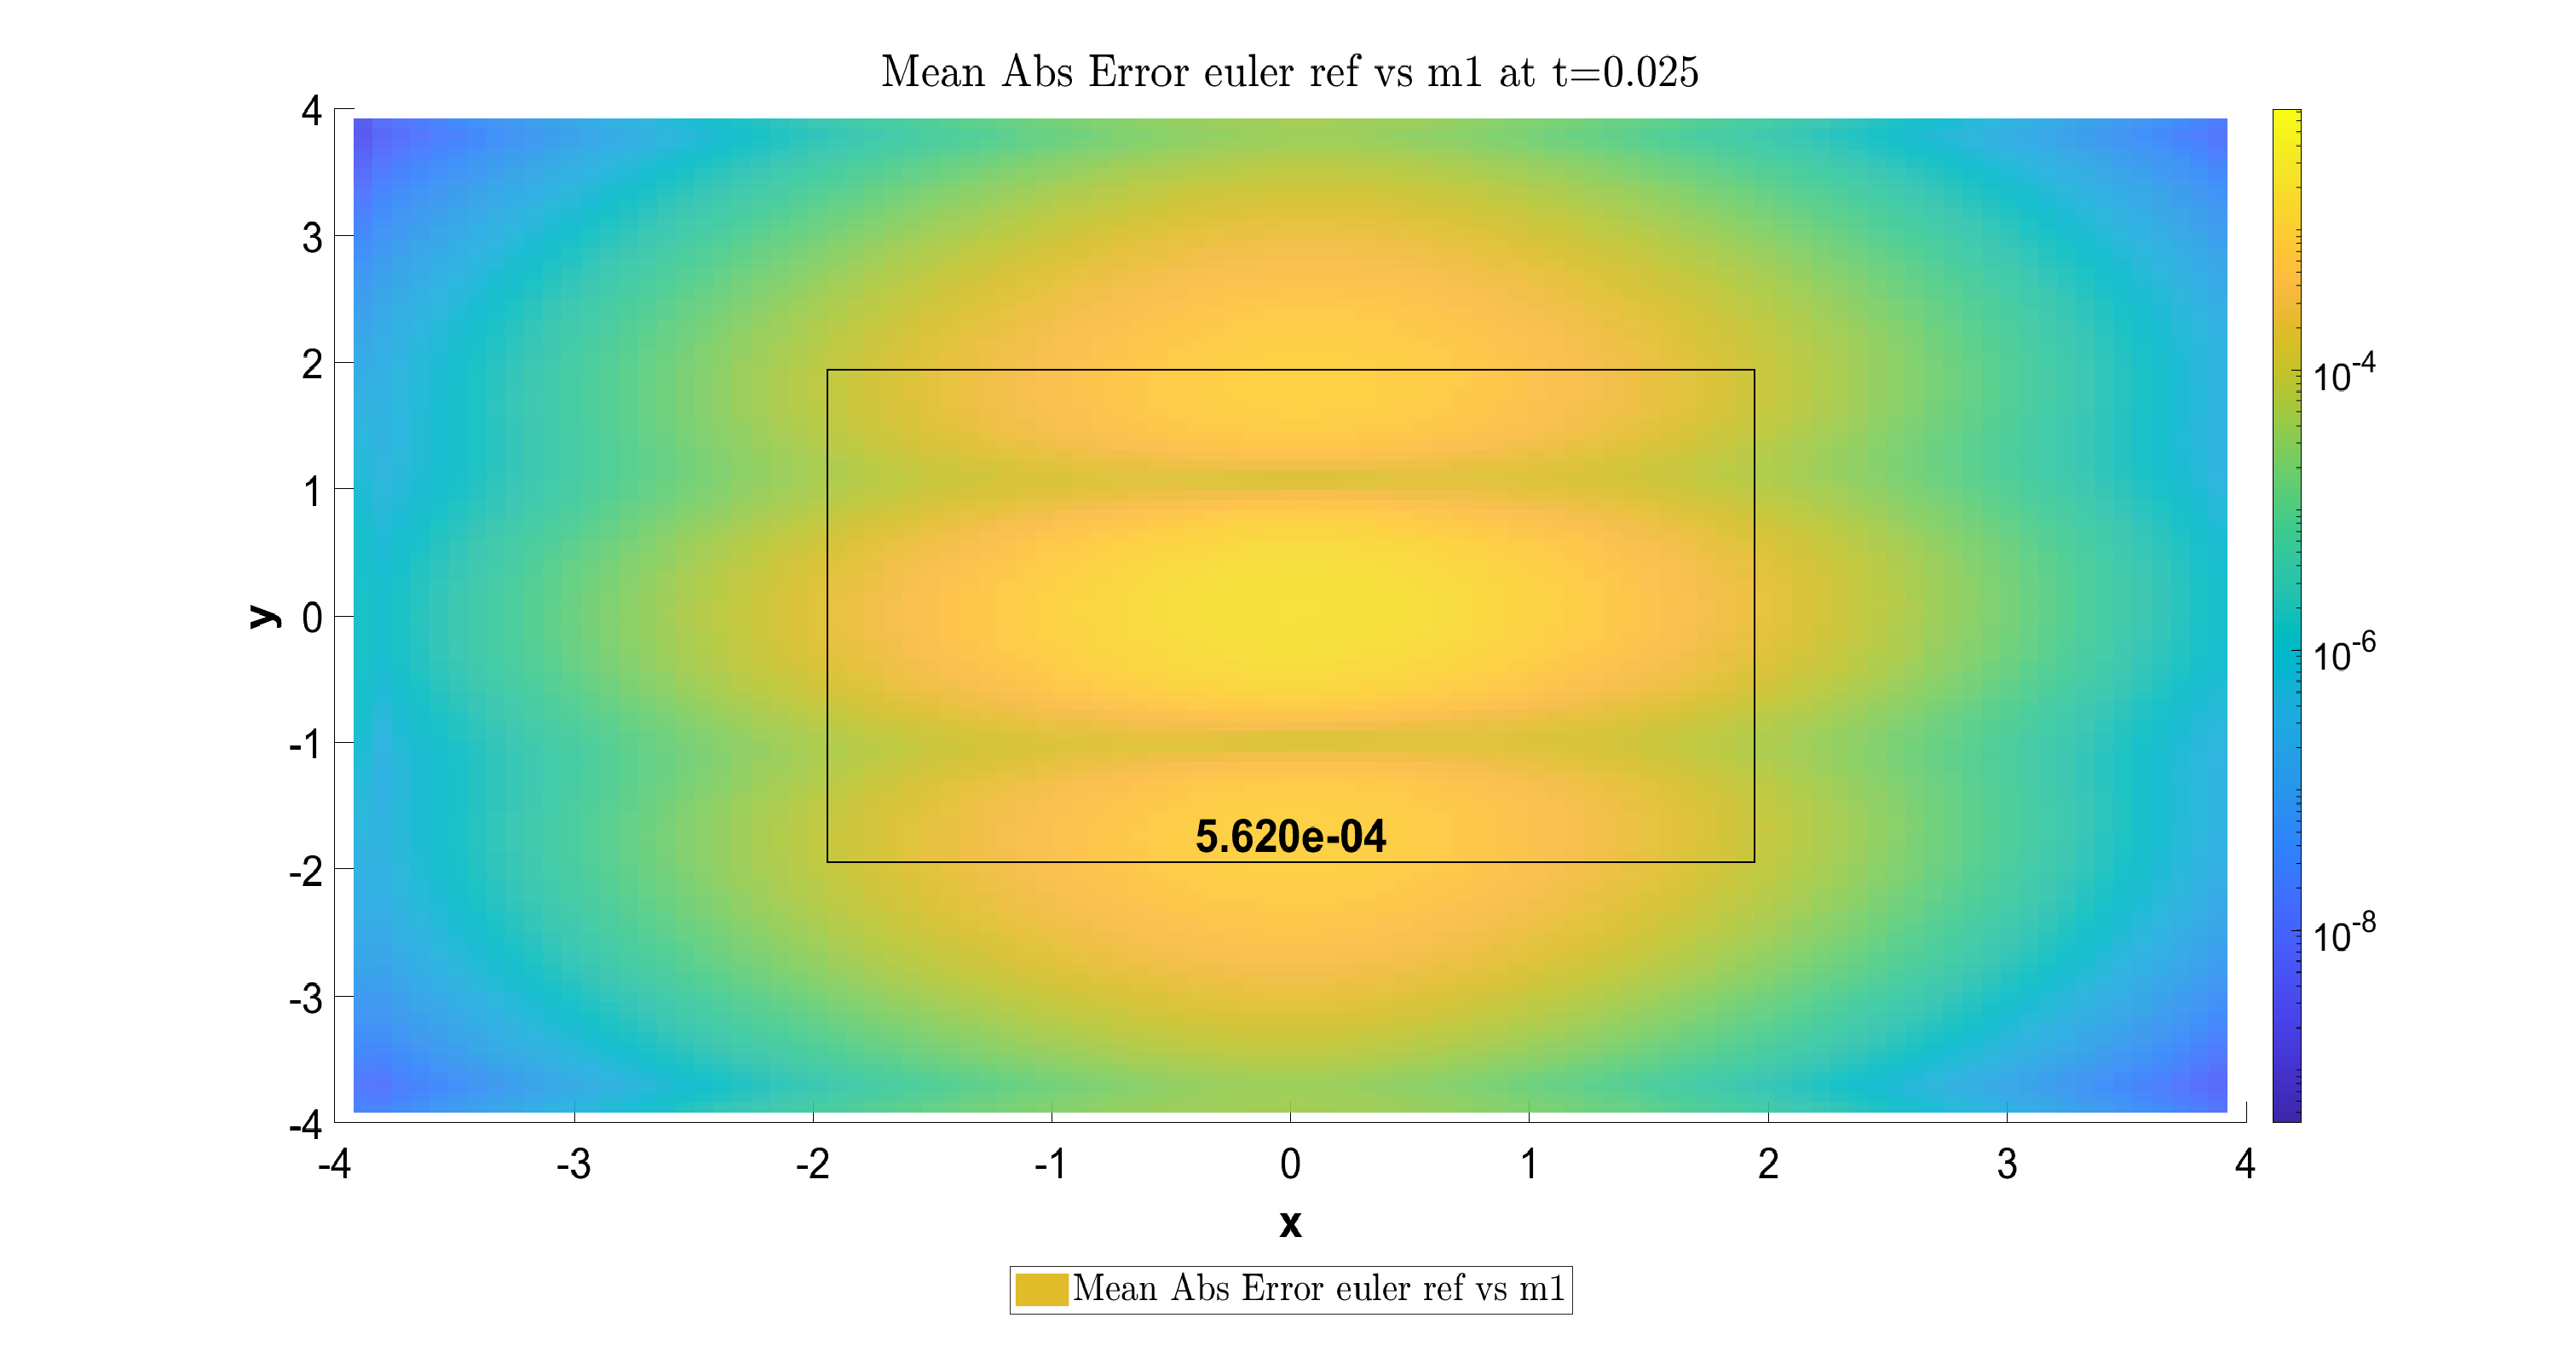
\includegraphics[width=.95\columnwidth]{CDF/CDFEulerRef_1}
\end{landscape}
\begin{landscape}
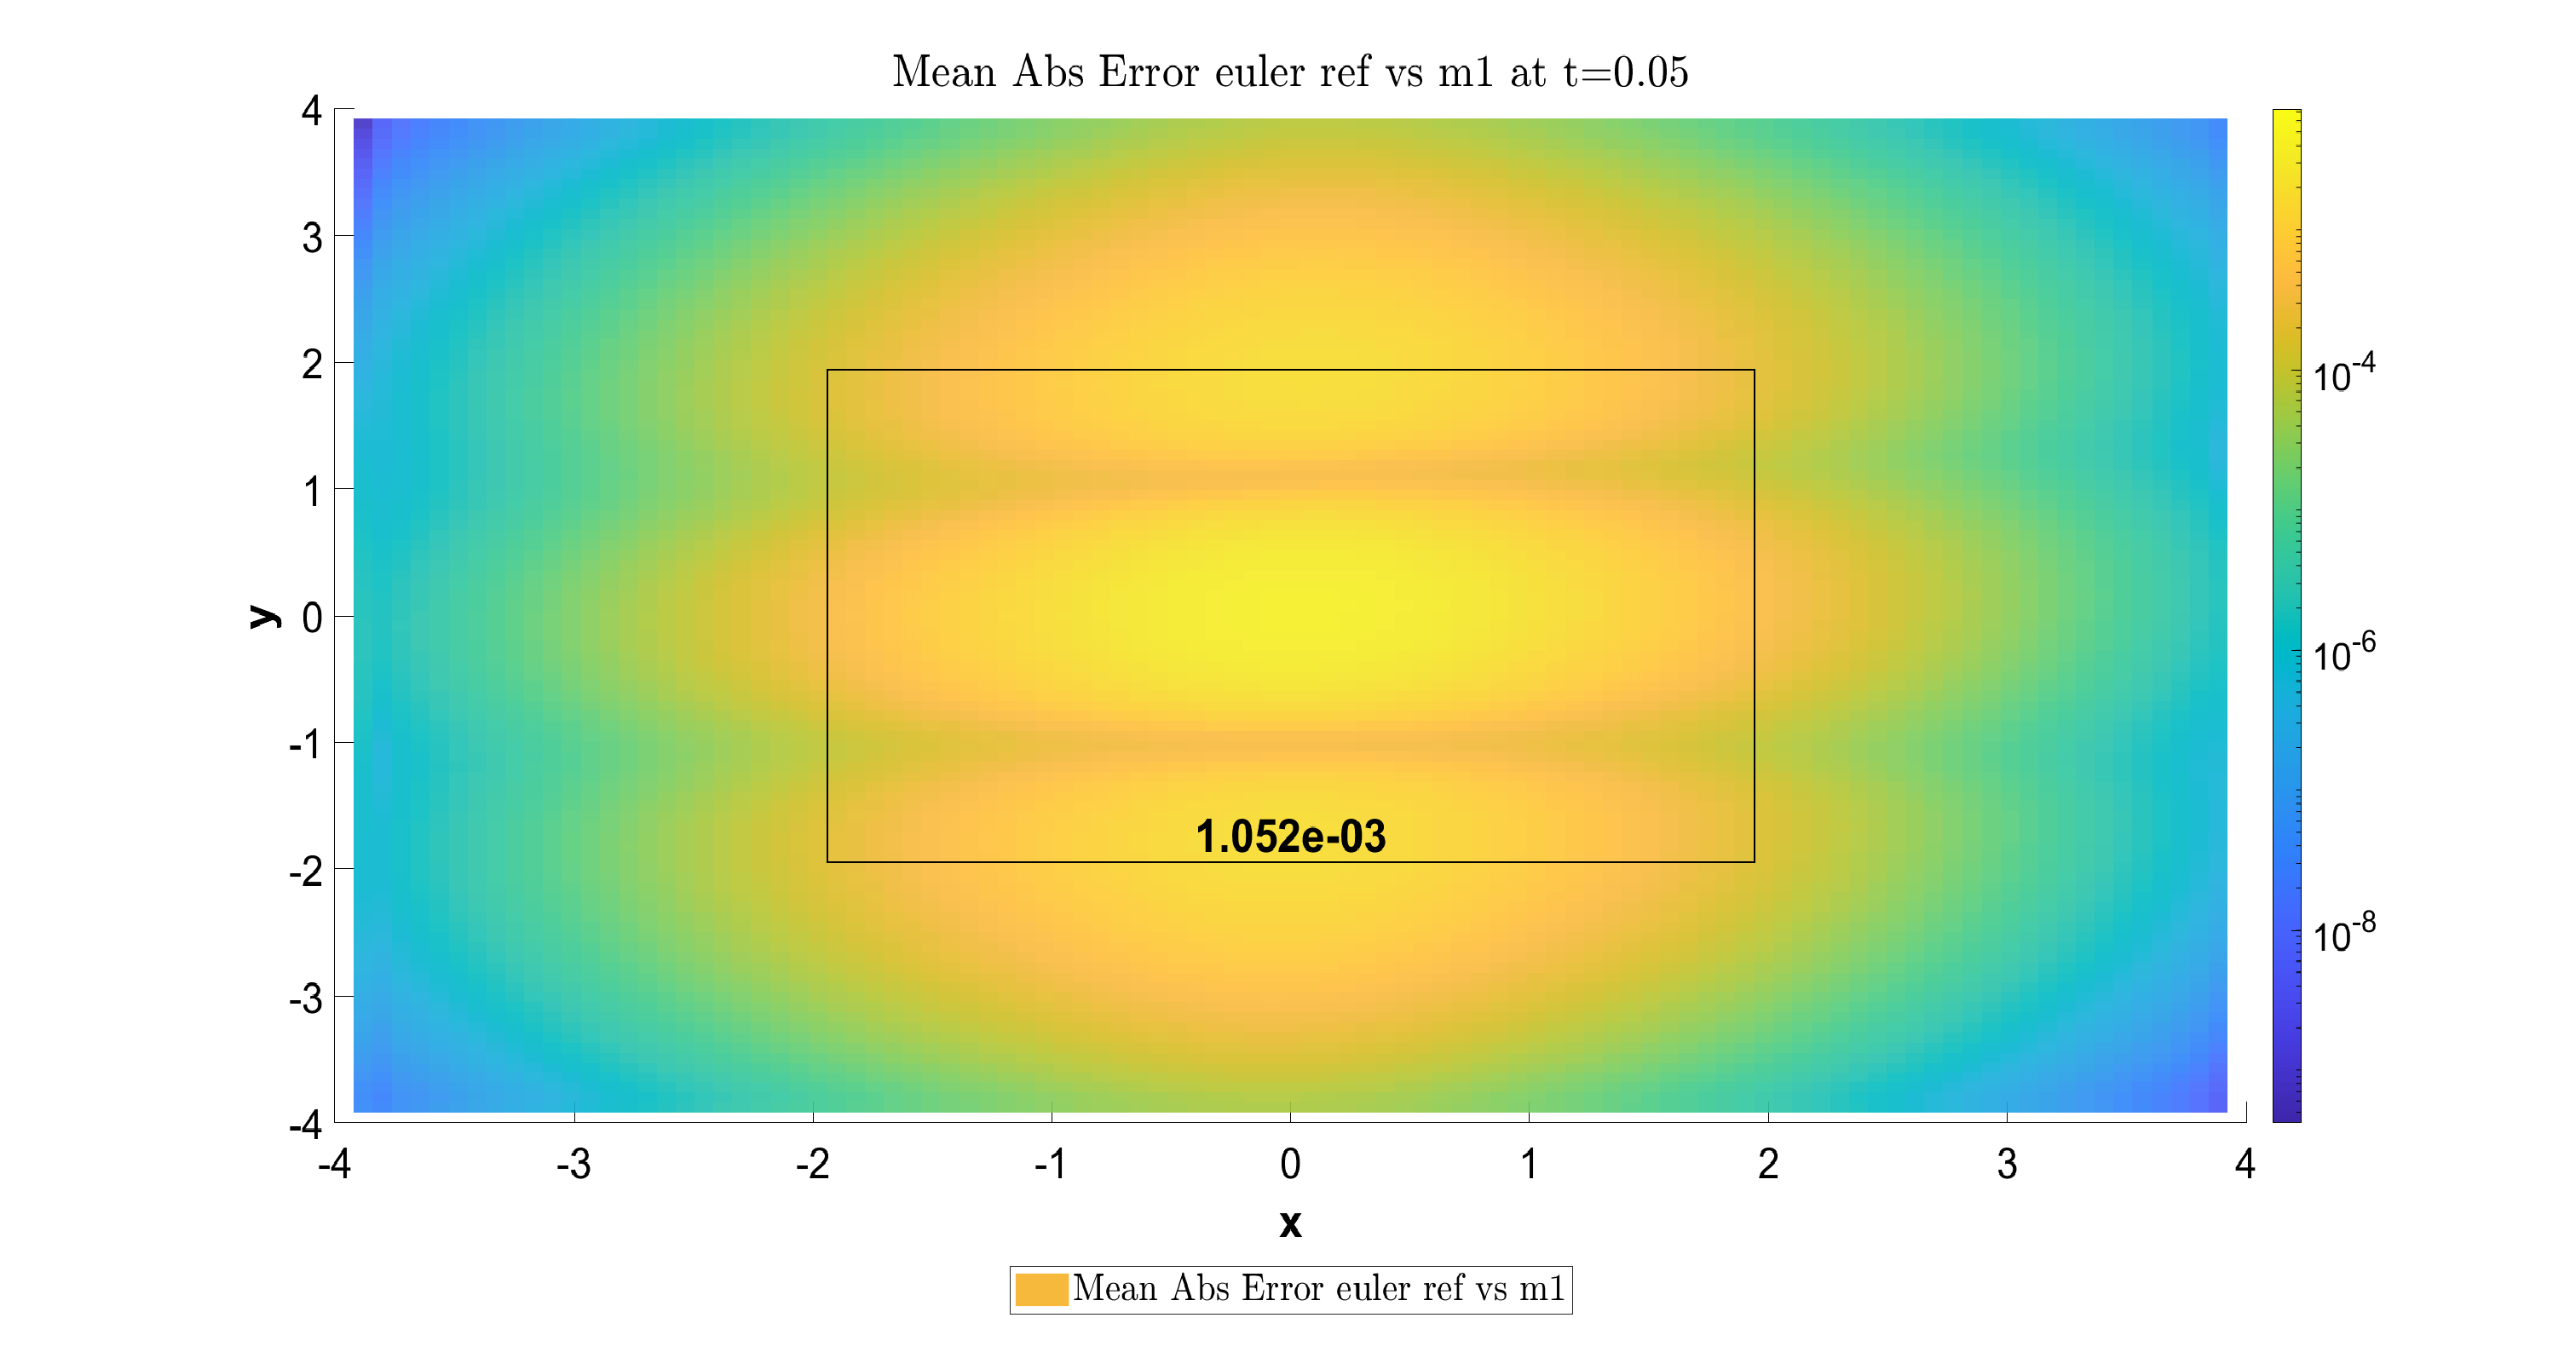
\includegraphics[width=.95\columnwidth]{CDF/CDFEulerRef_2}
\end{landscape}
\begin{landscape}
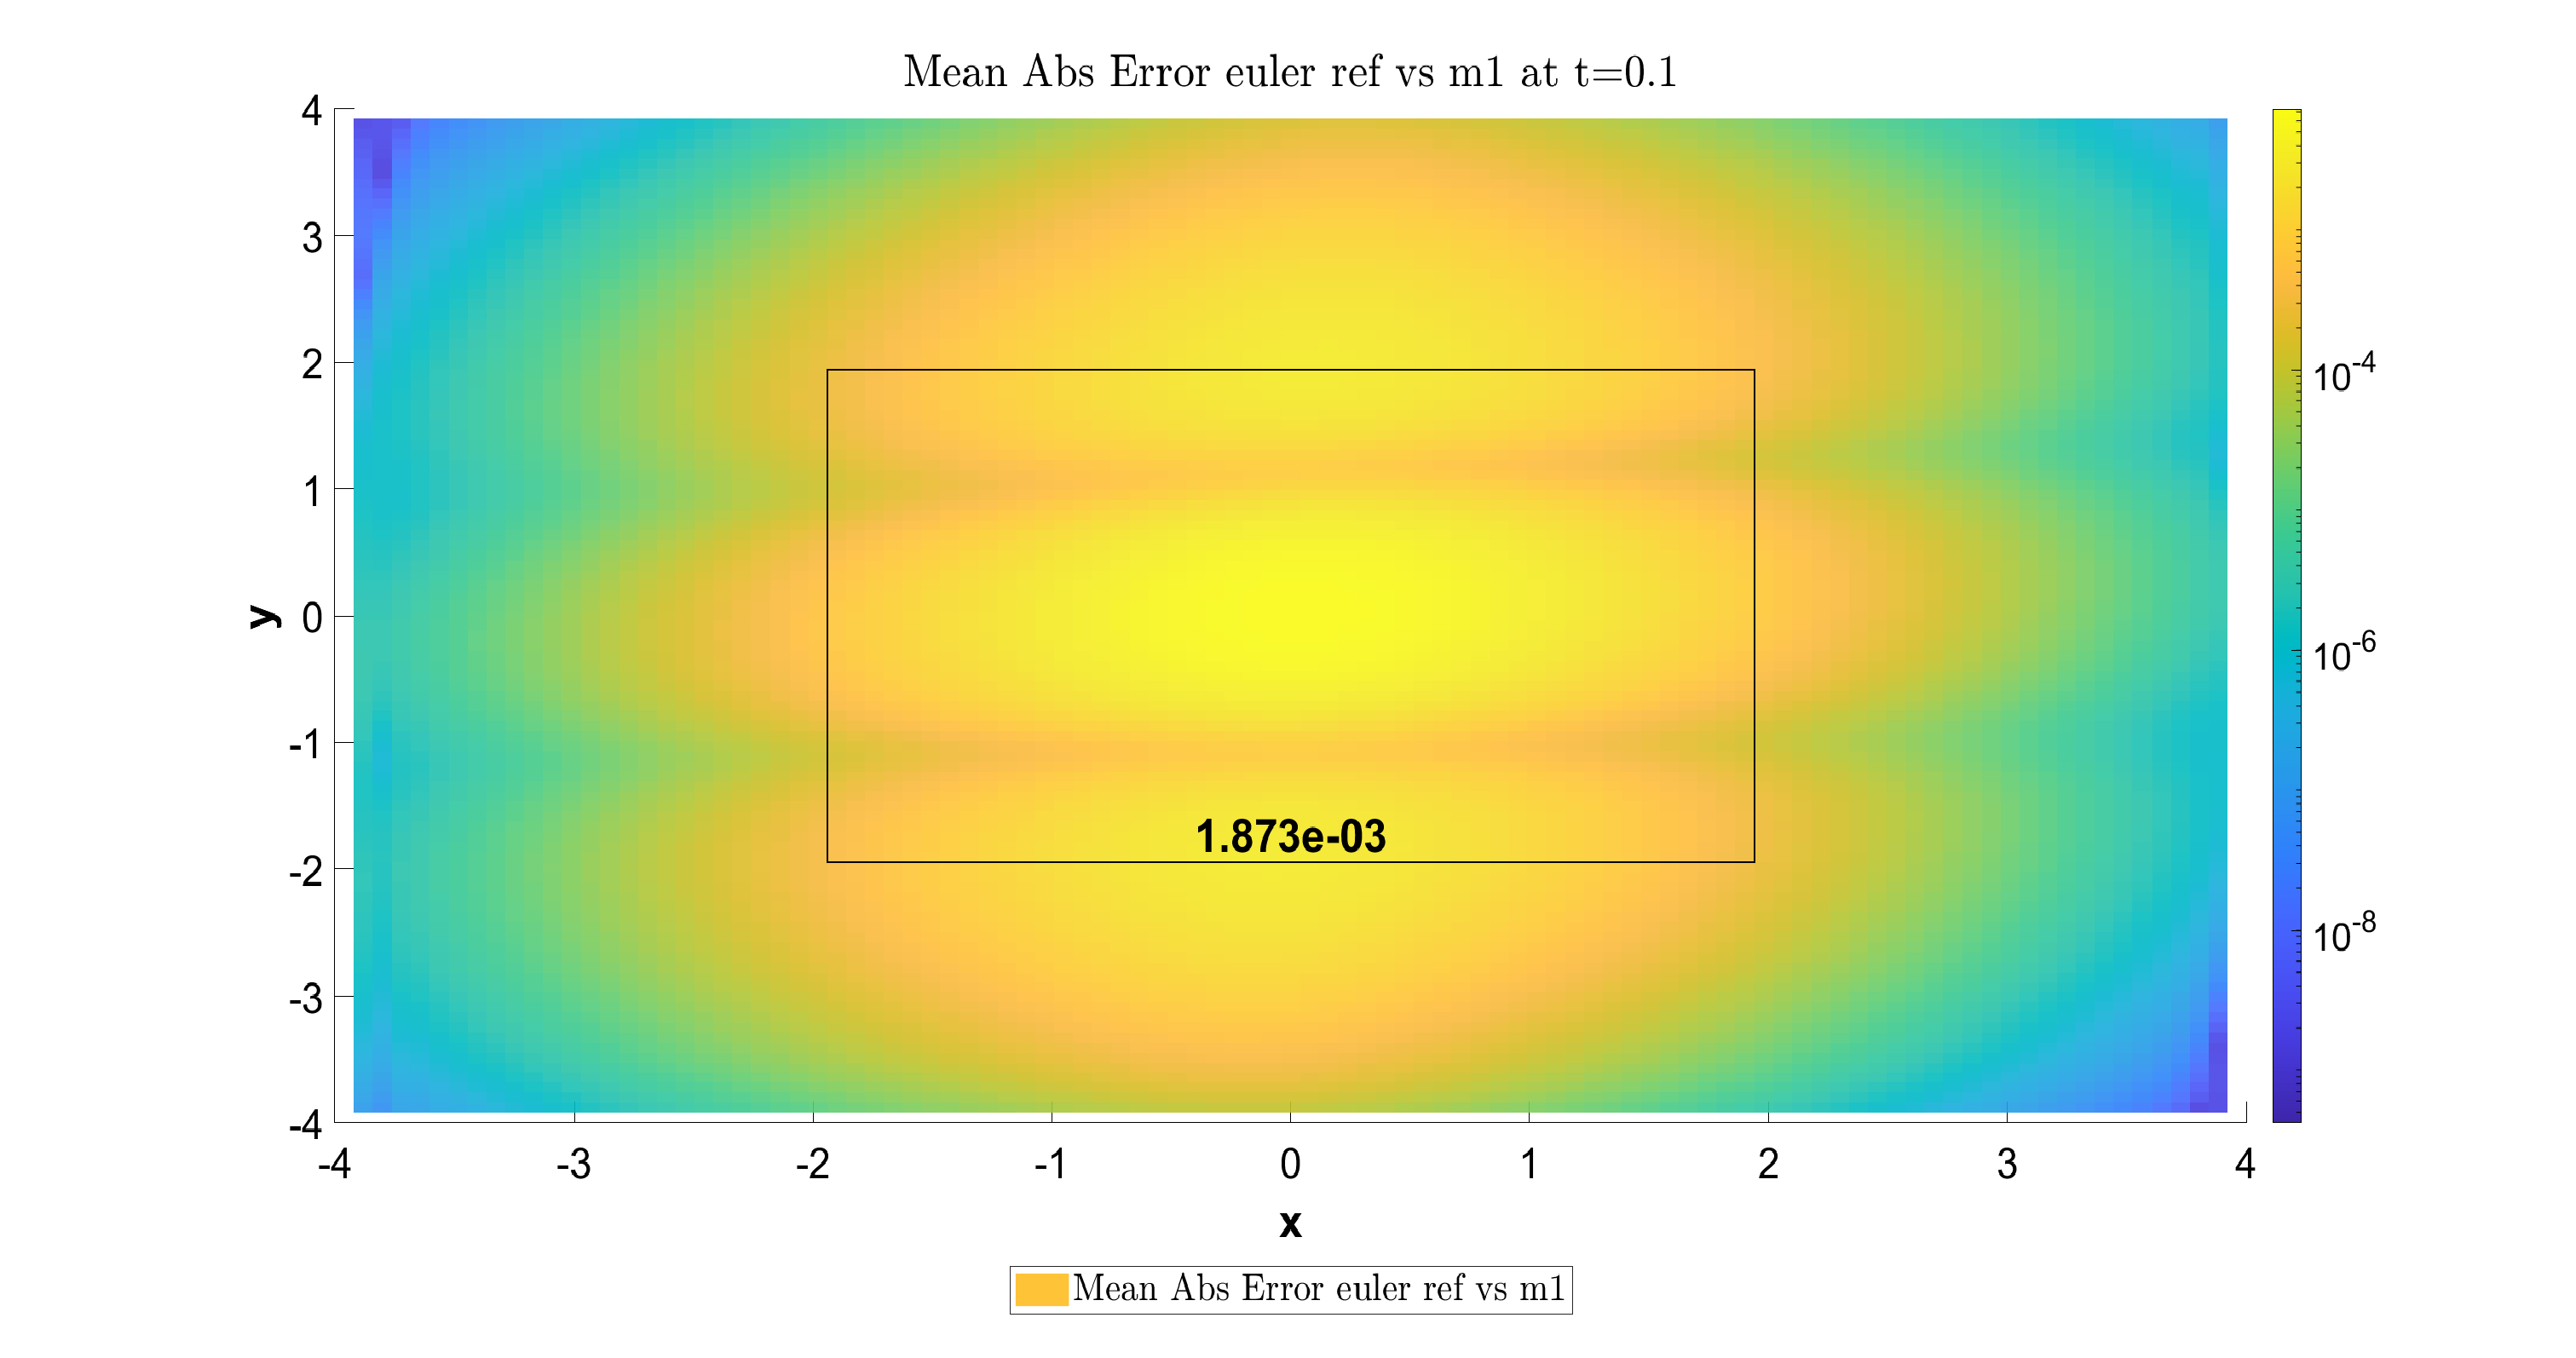
\includegraphics[width=.95\columnwidth]{CDF/CDFEulerRef_3}
\end{landscape}
\begin{landscape}
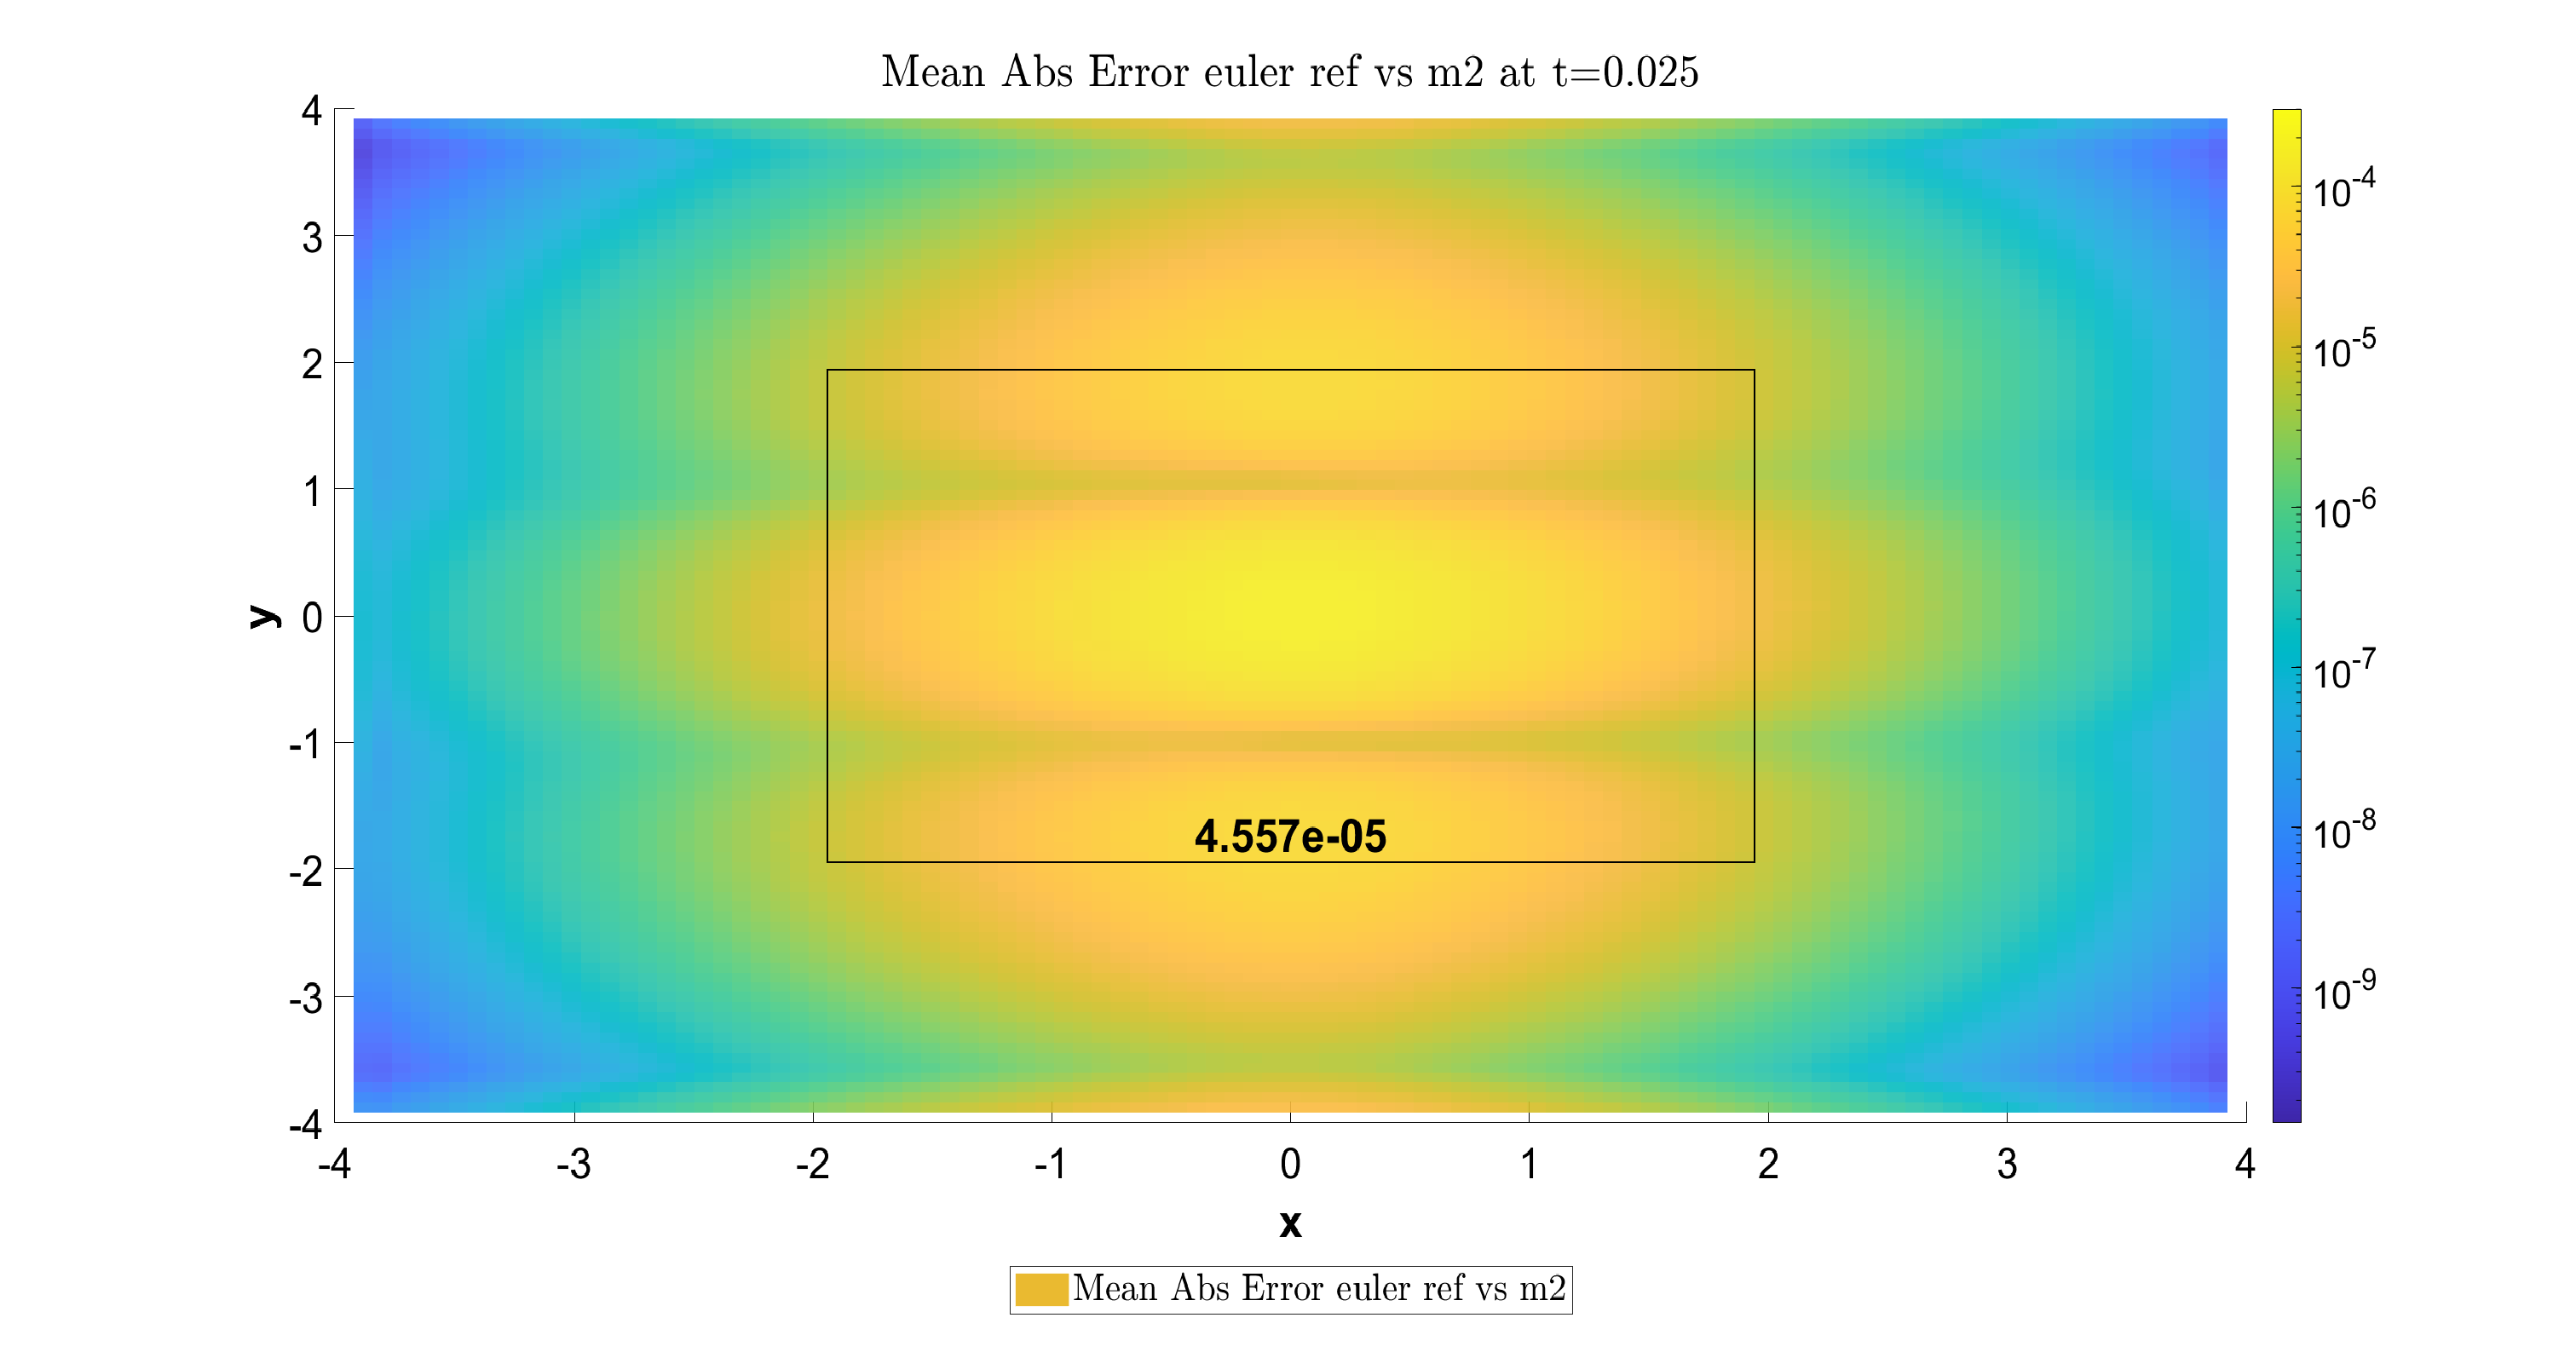
\includegraphics[width=.95\columnwidth]{CDF/CDFEulerRef_4}
\end{landscape}
\begin{landscape}
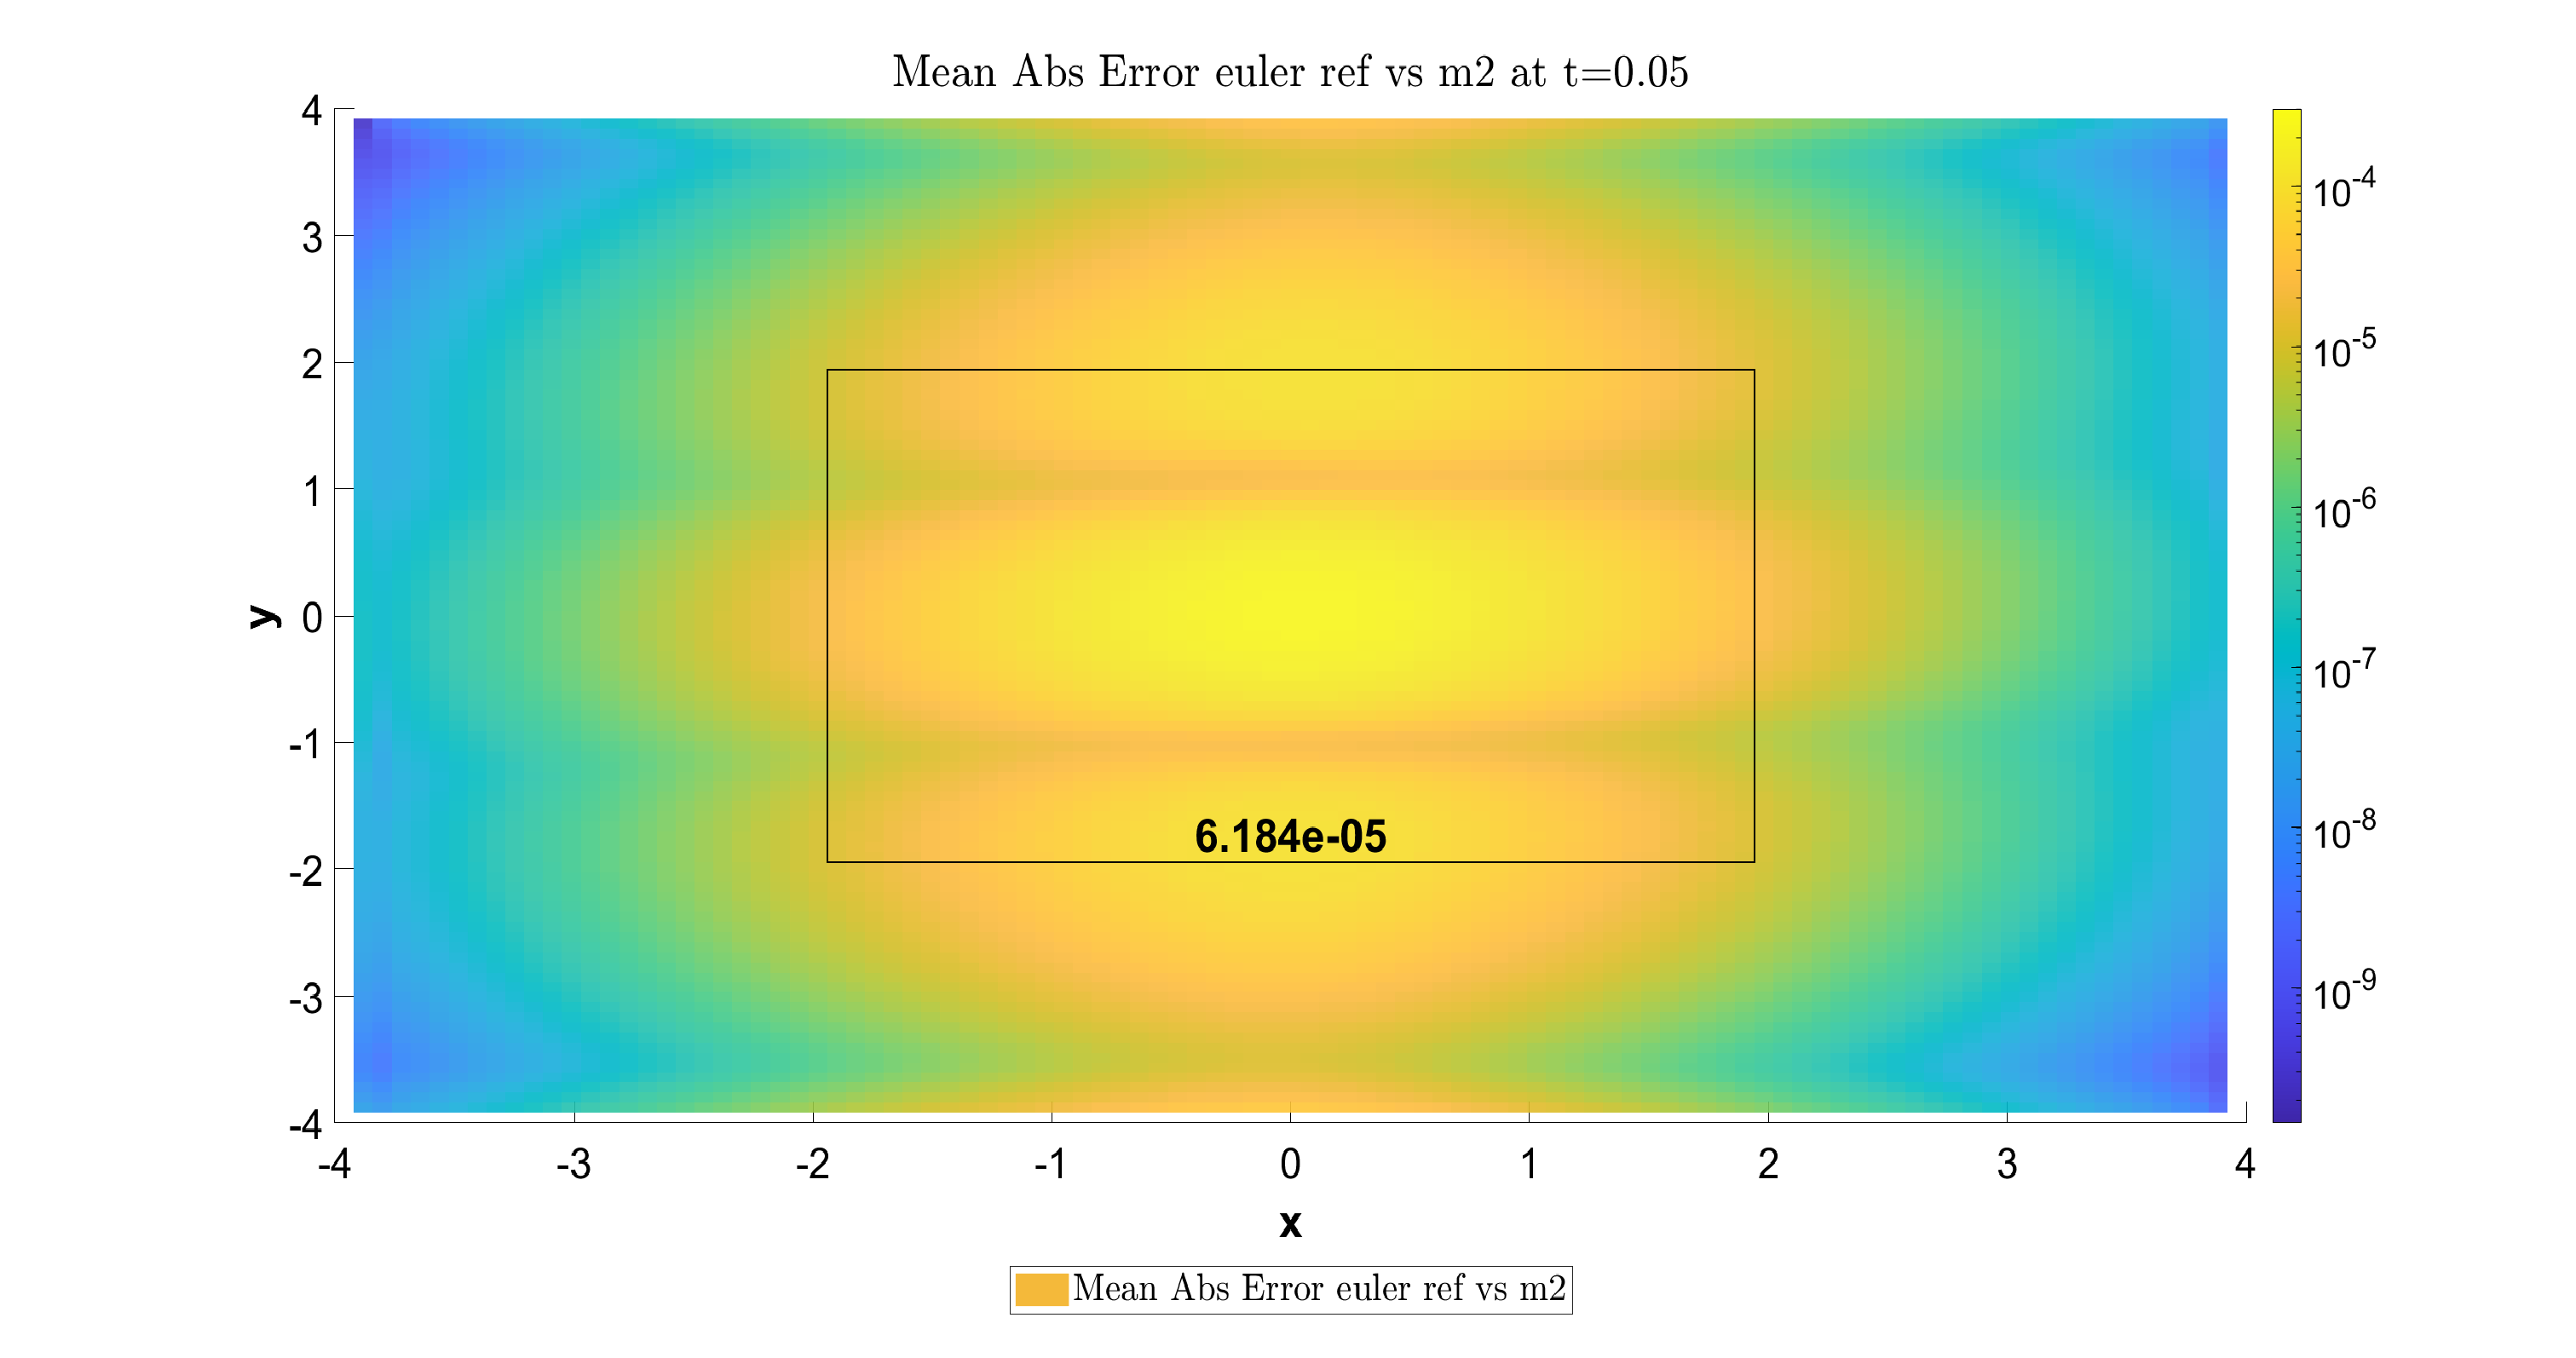
\includegraphics[width=.95\columnwidth]{CDF/CDFEulerRef_5}
\end{landscape}
\begin{landscape}
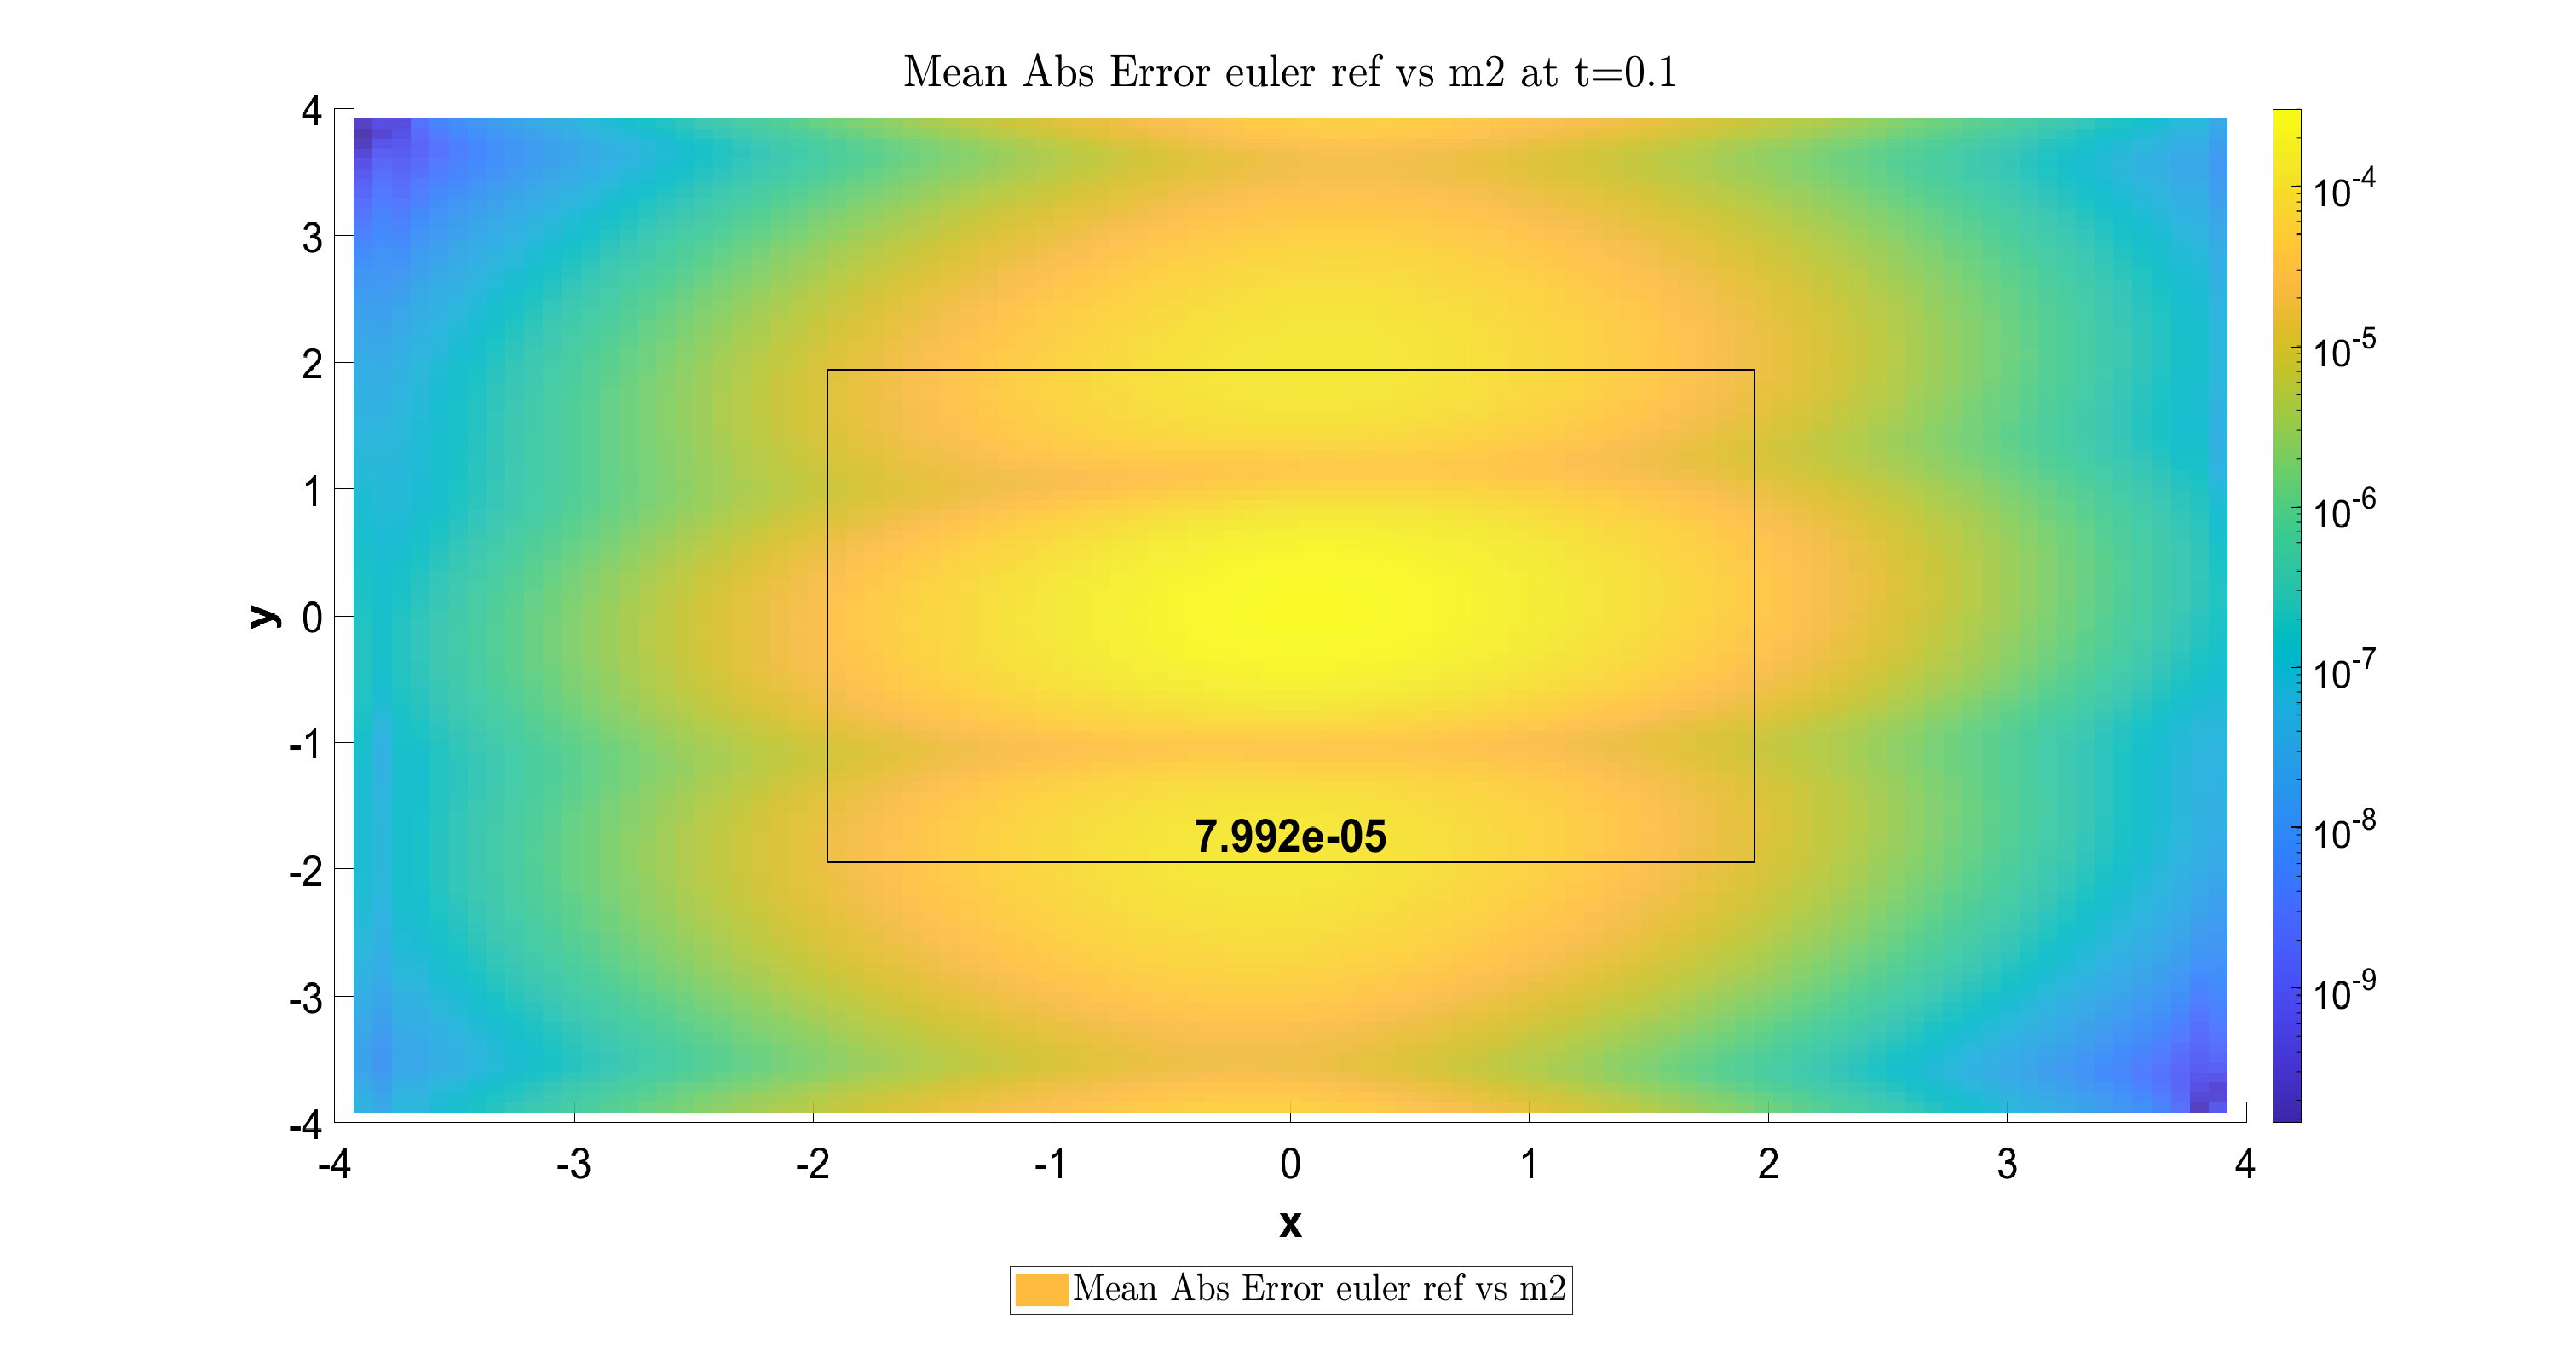
\includegraphics[width=.95\columnwidth]{CDF/CDFEulerRef_6}
\end{landscape}
\begin{landscape}
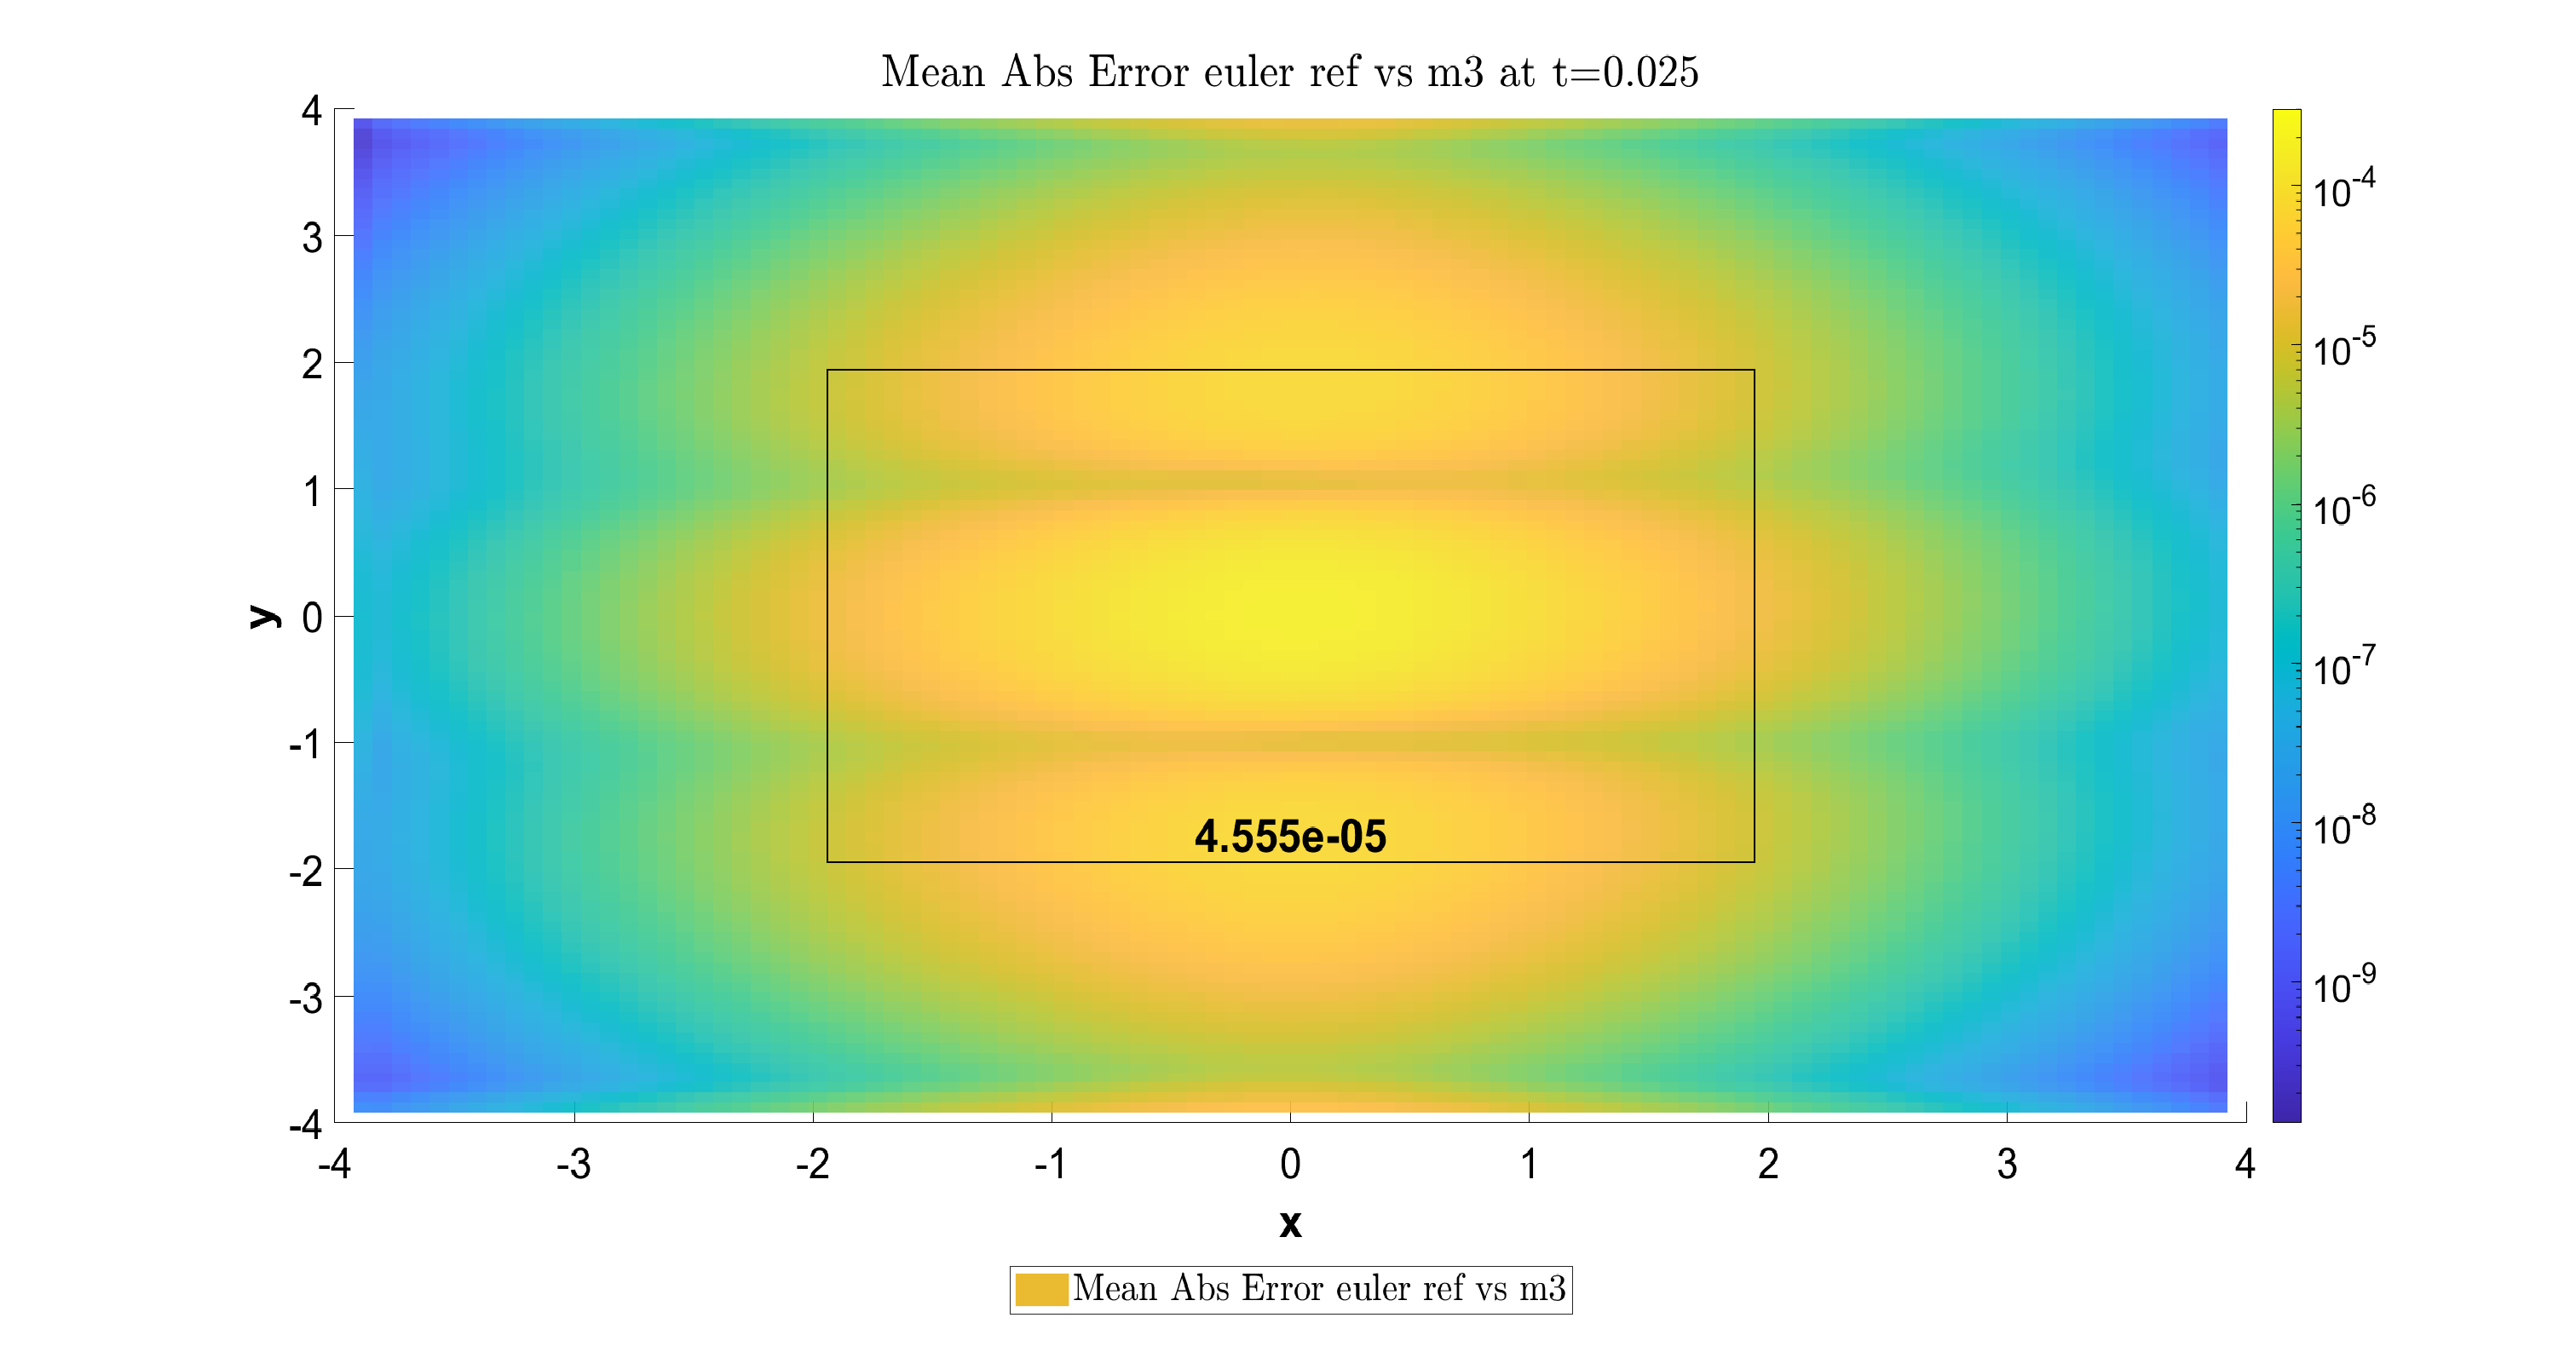
\includegraphics[width=.95\columnwidth]{CDF/CDFEulerRef_7}
\end{landscape}
\begin{landscape}
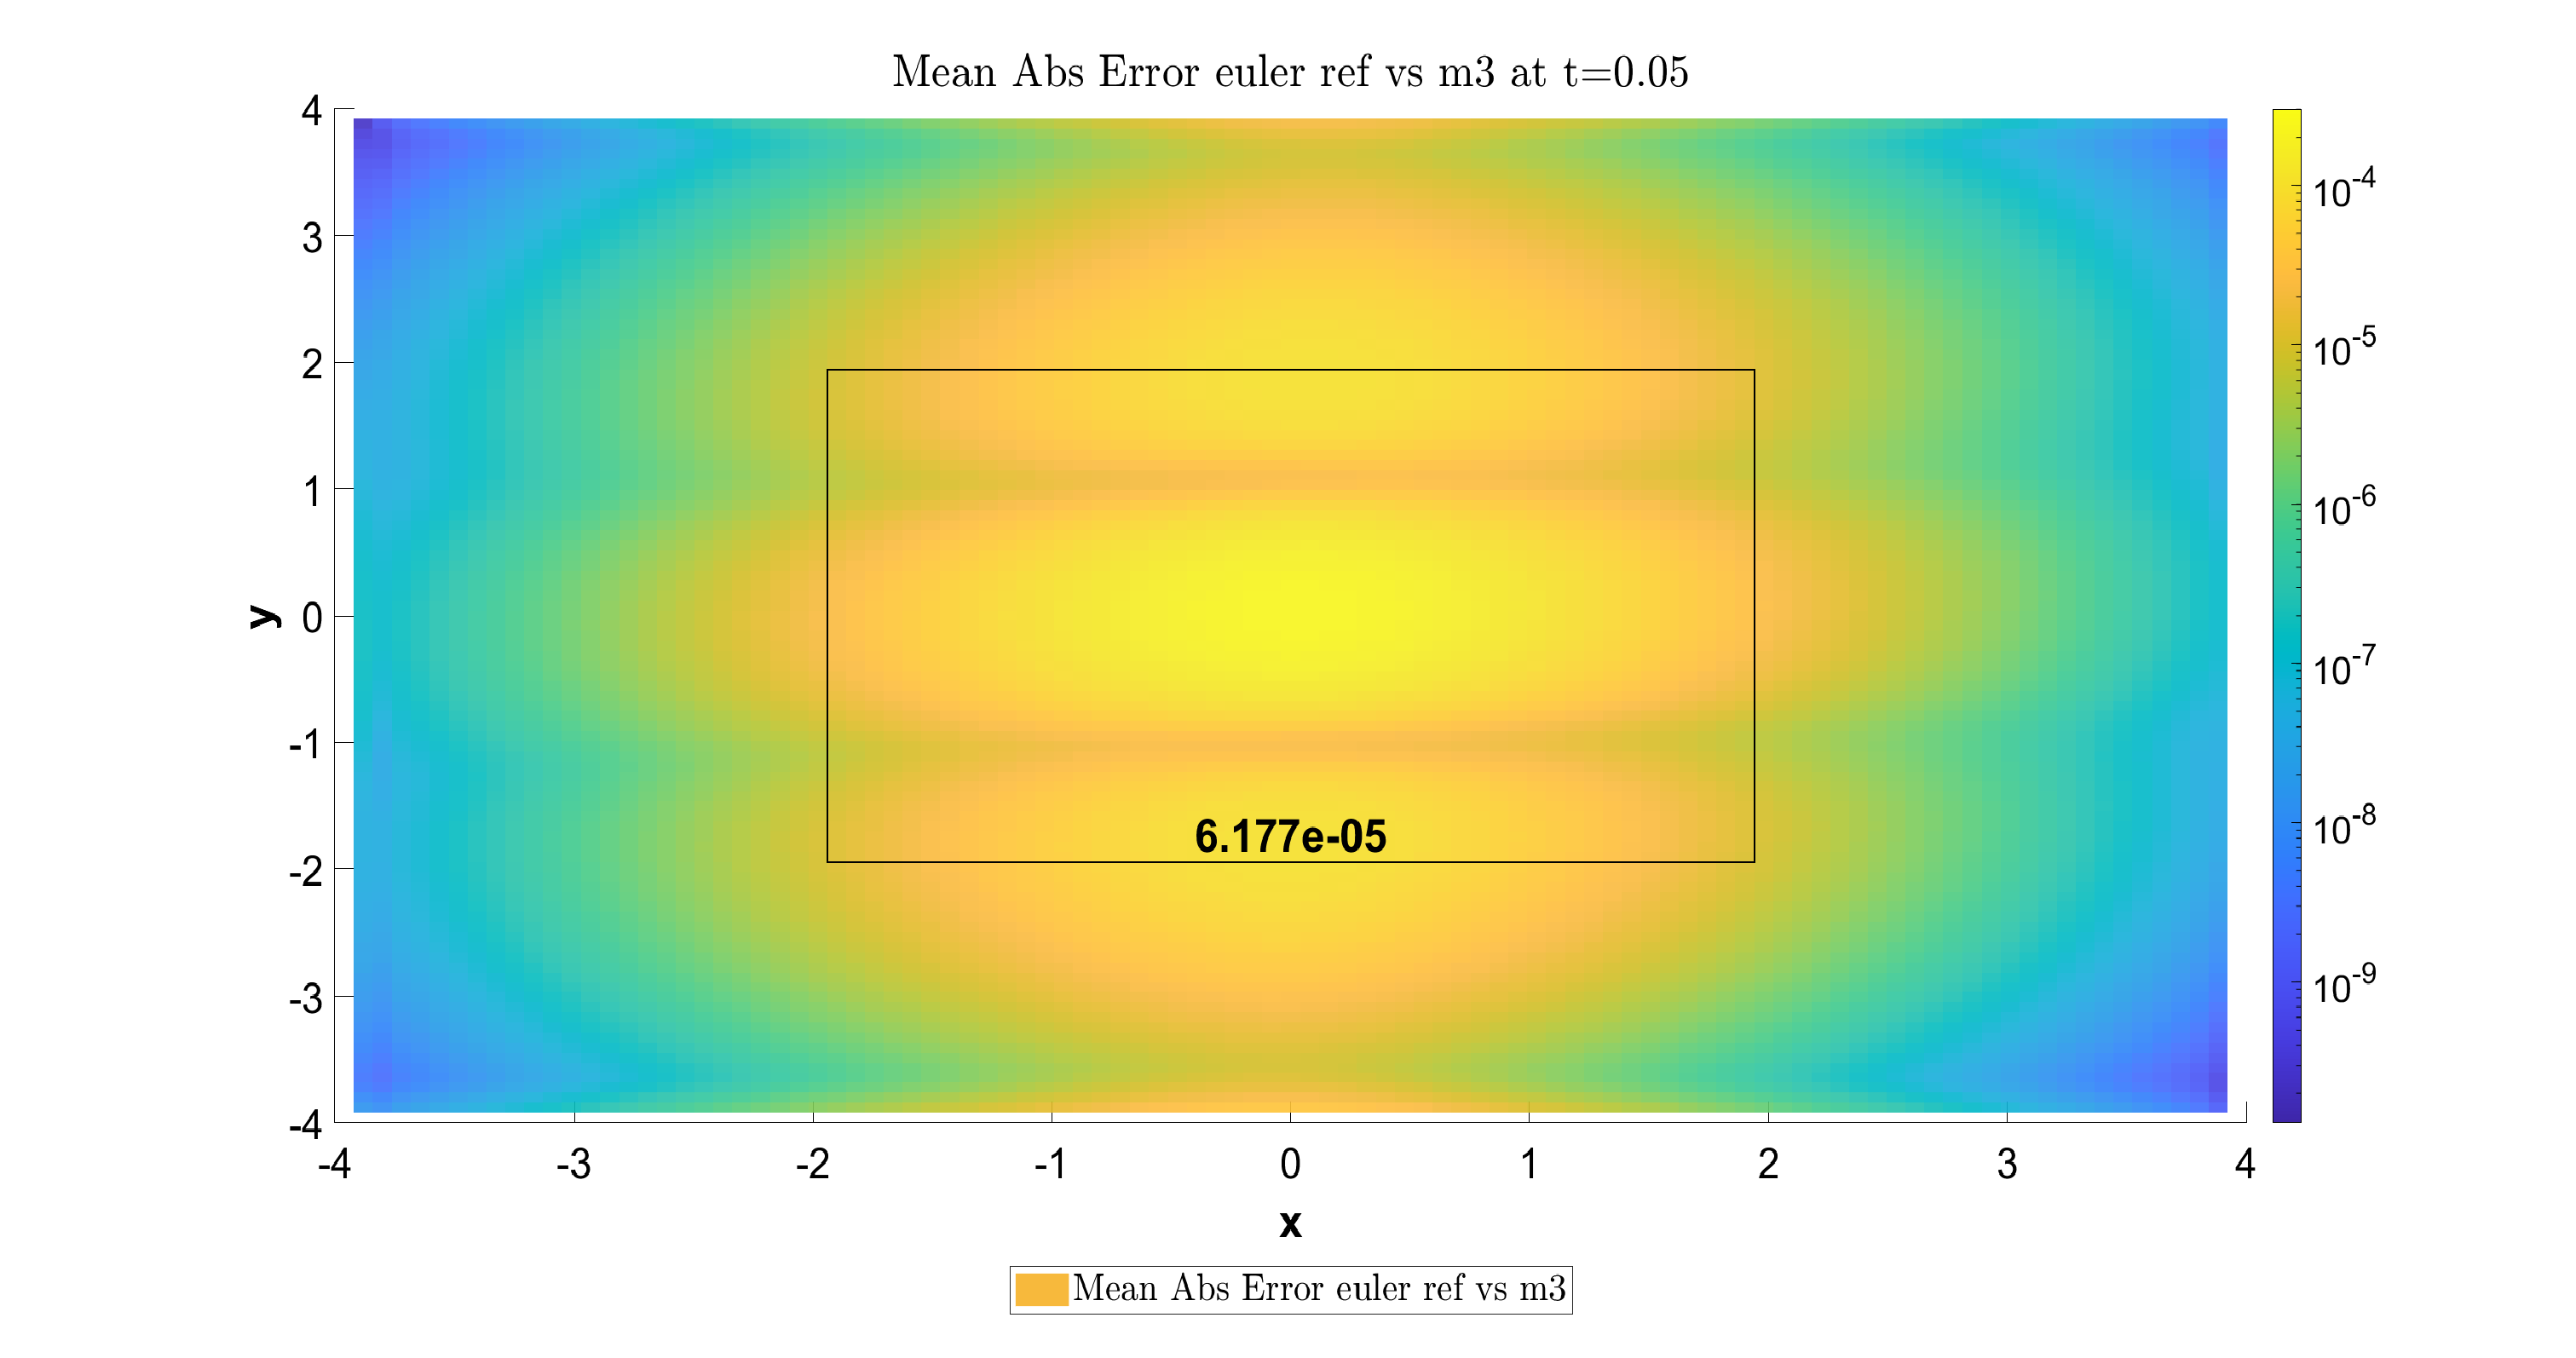
\includegraphics[width=.95\columnwidth]{CDF/CDFEulerRef_8}
\end{landscape}
\begin{landscape}
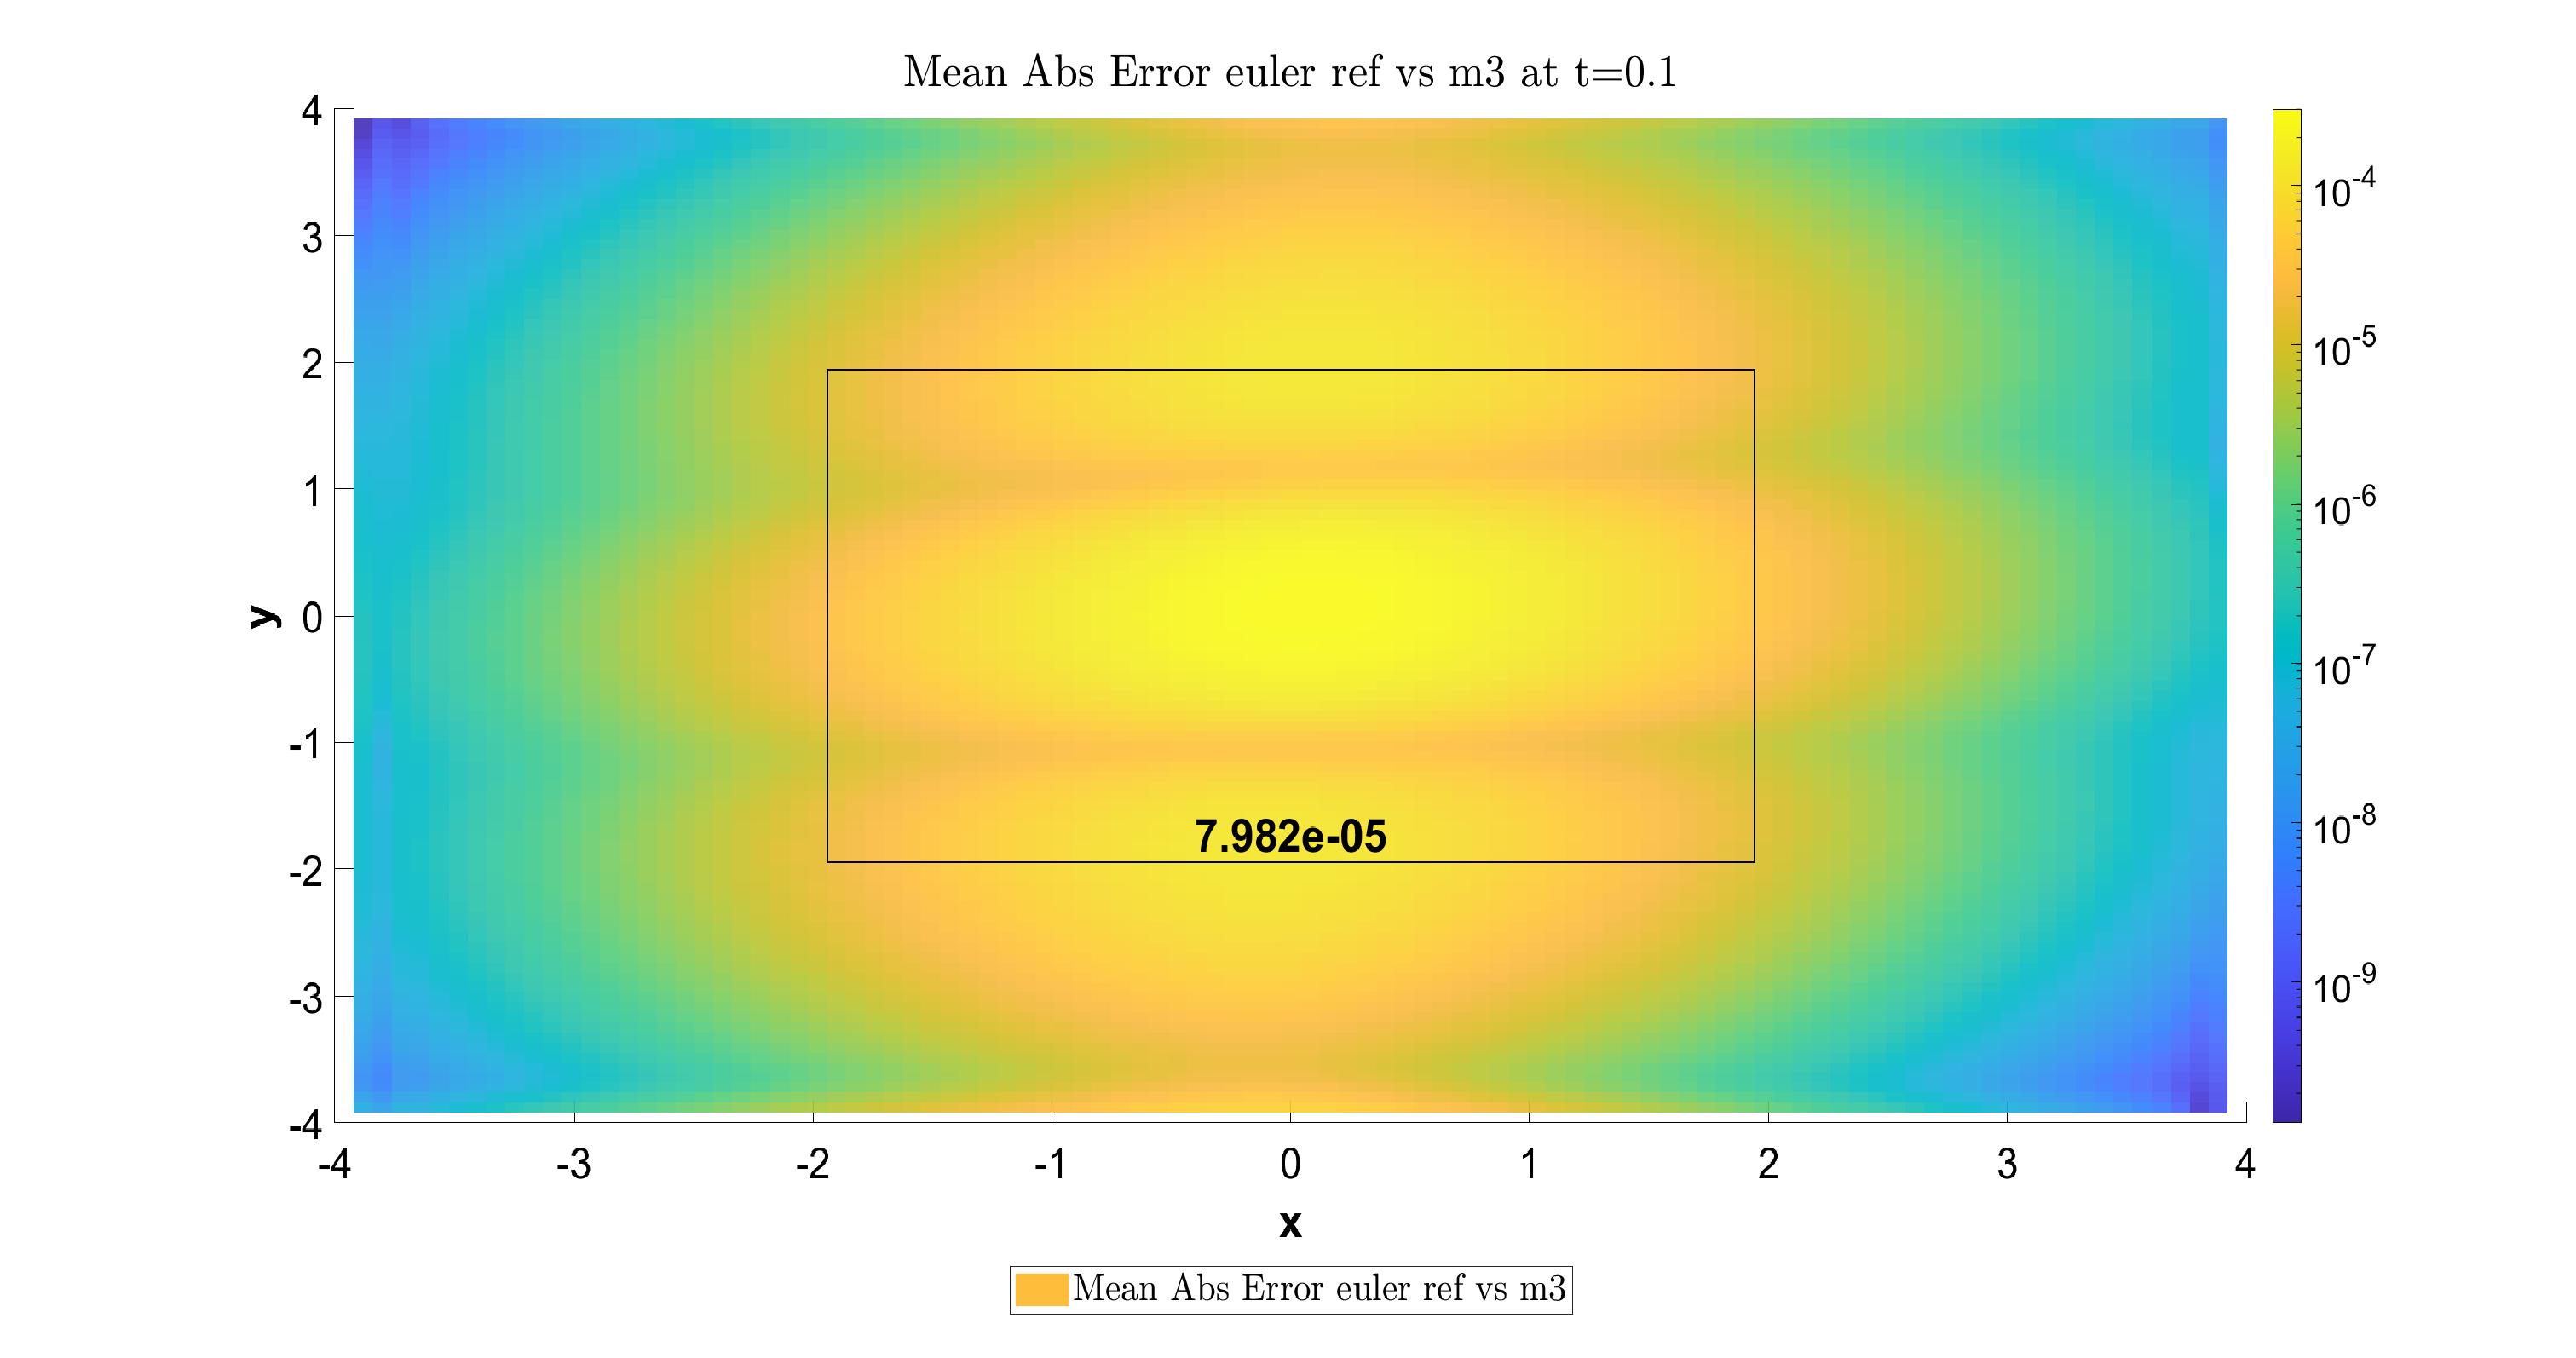
\includegraphics[width=.95\columnwidth]{CDF/CDFEulerRef_9}
\end{landscape}
\begin{landscape}
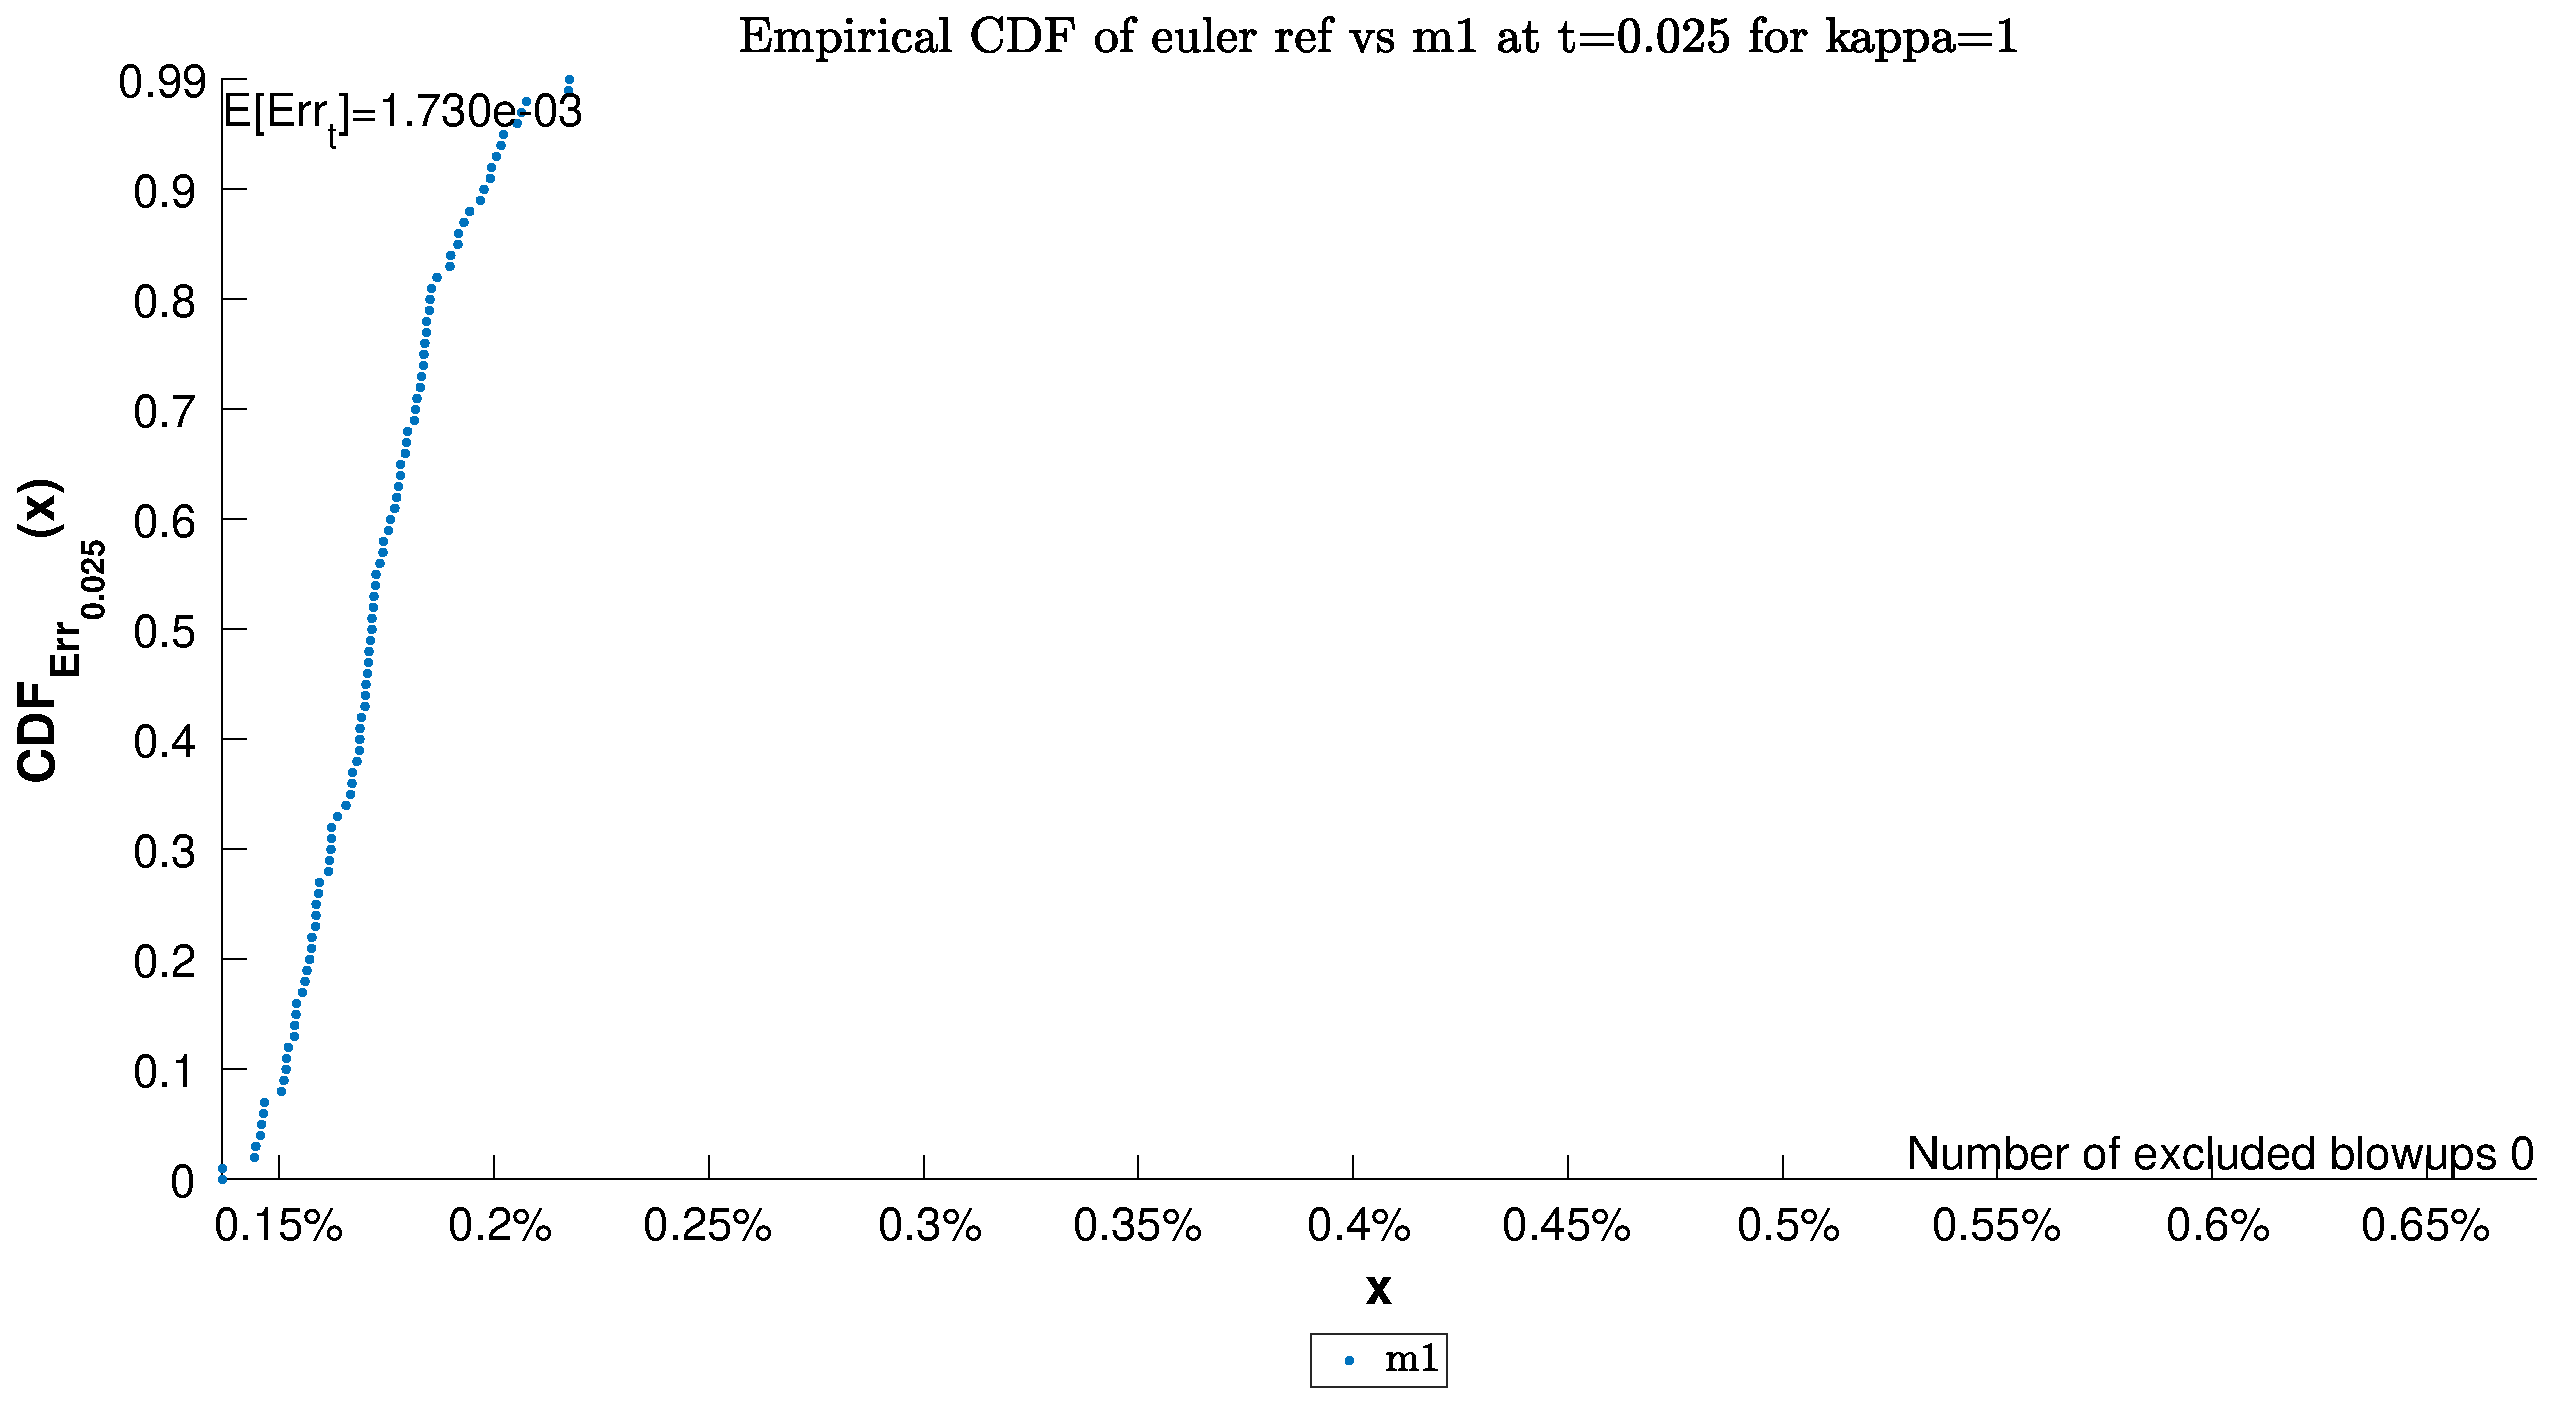
\includegraphics[width=.95\columnwidth]{CDF/CDFEulerRef_10}
\end{landscape}
\begin{landscape}
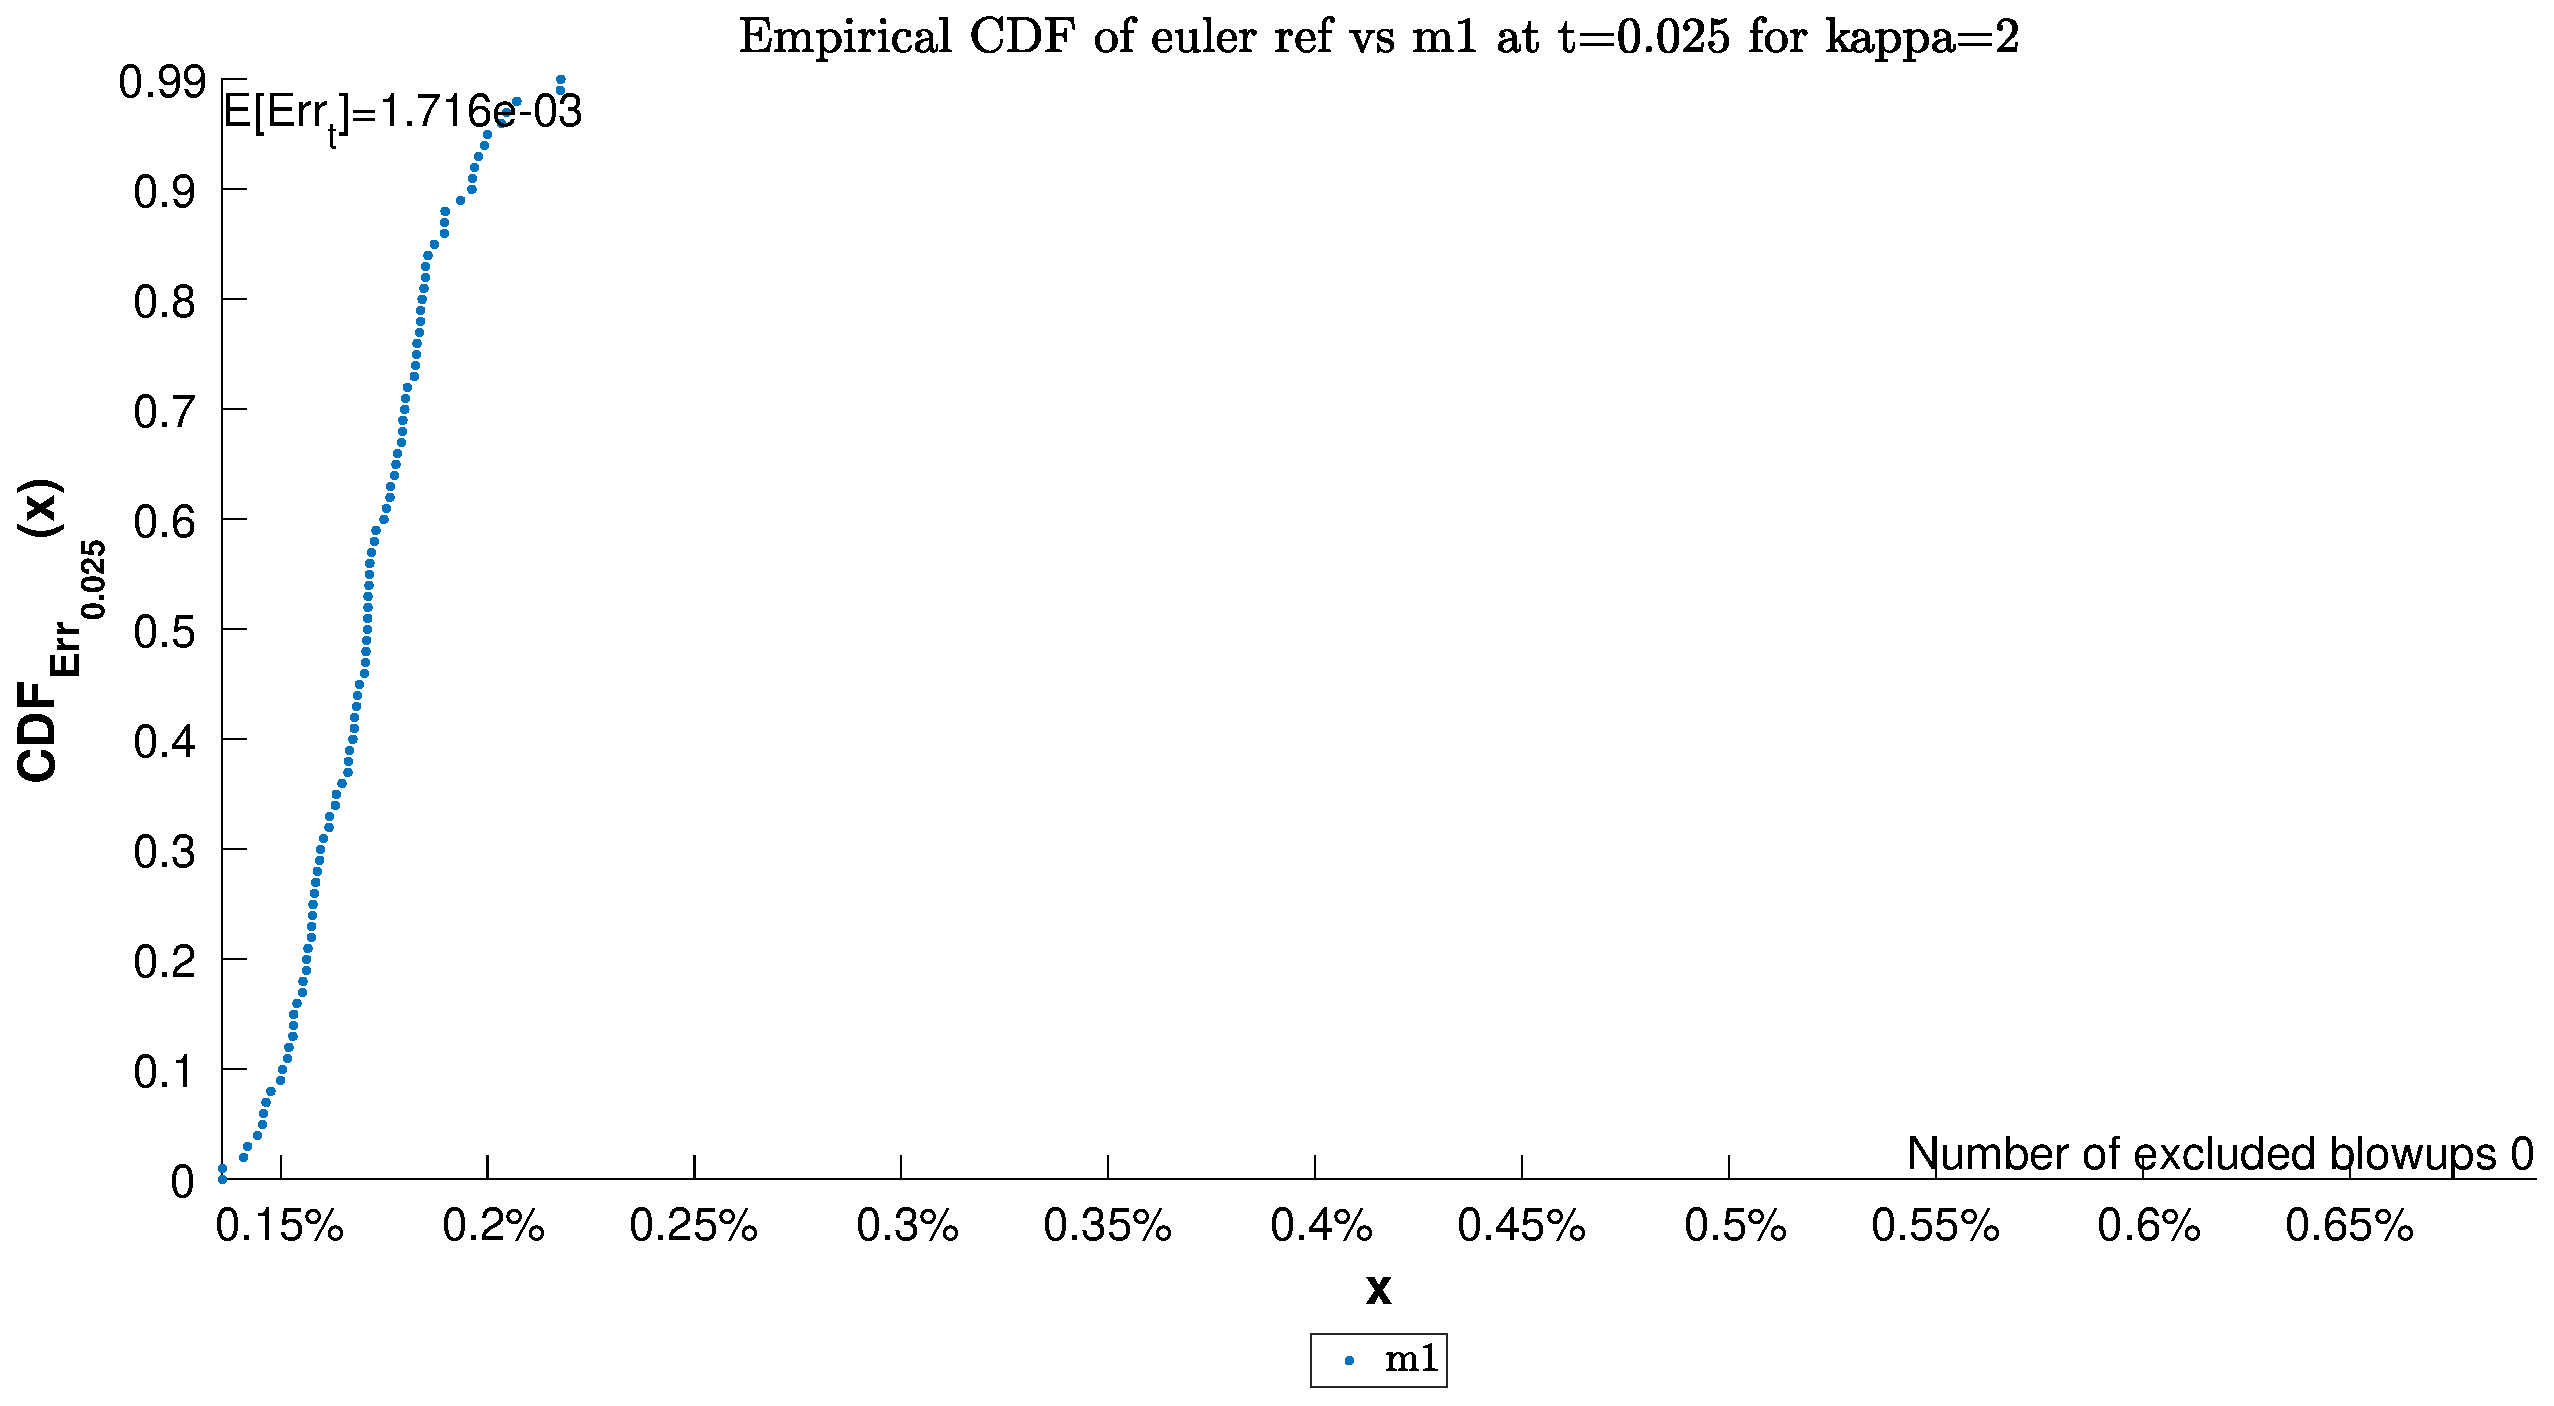
\includegraphics[width=.95\columnwidth]{CDF/CDFEulerRef_11}
\end{landscape}
\begin{landscape}
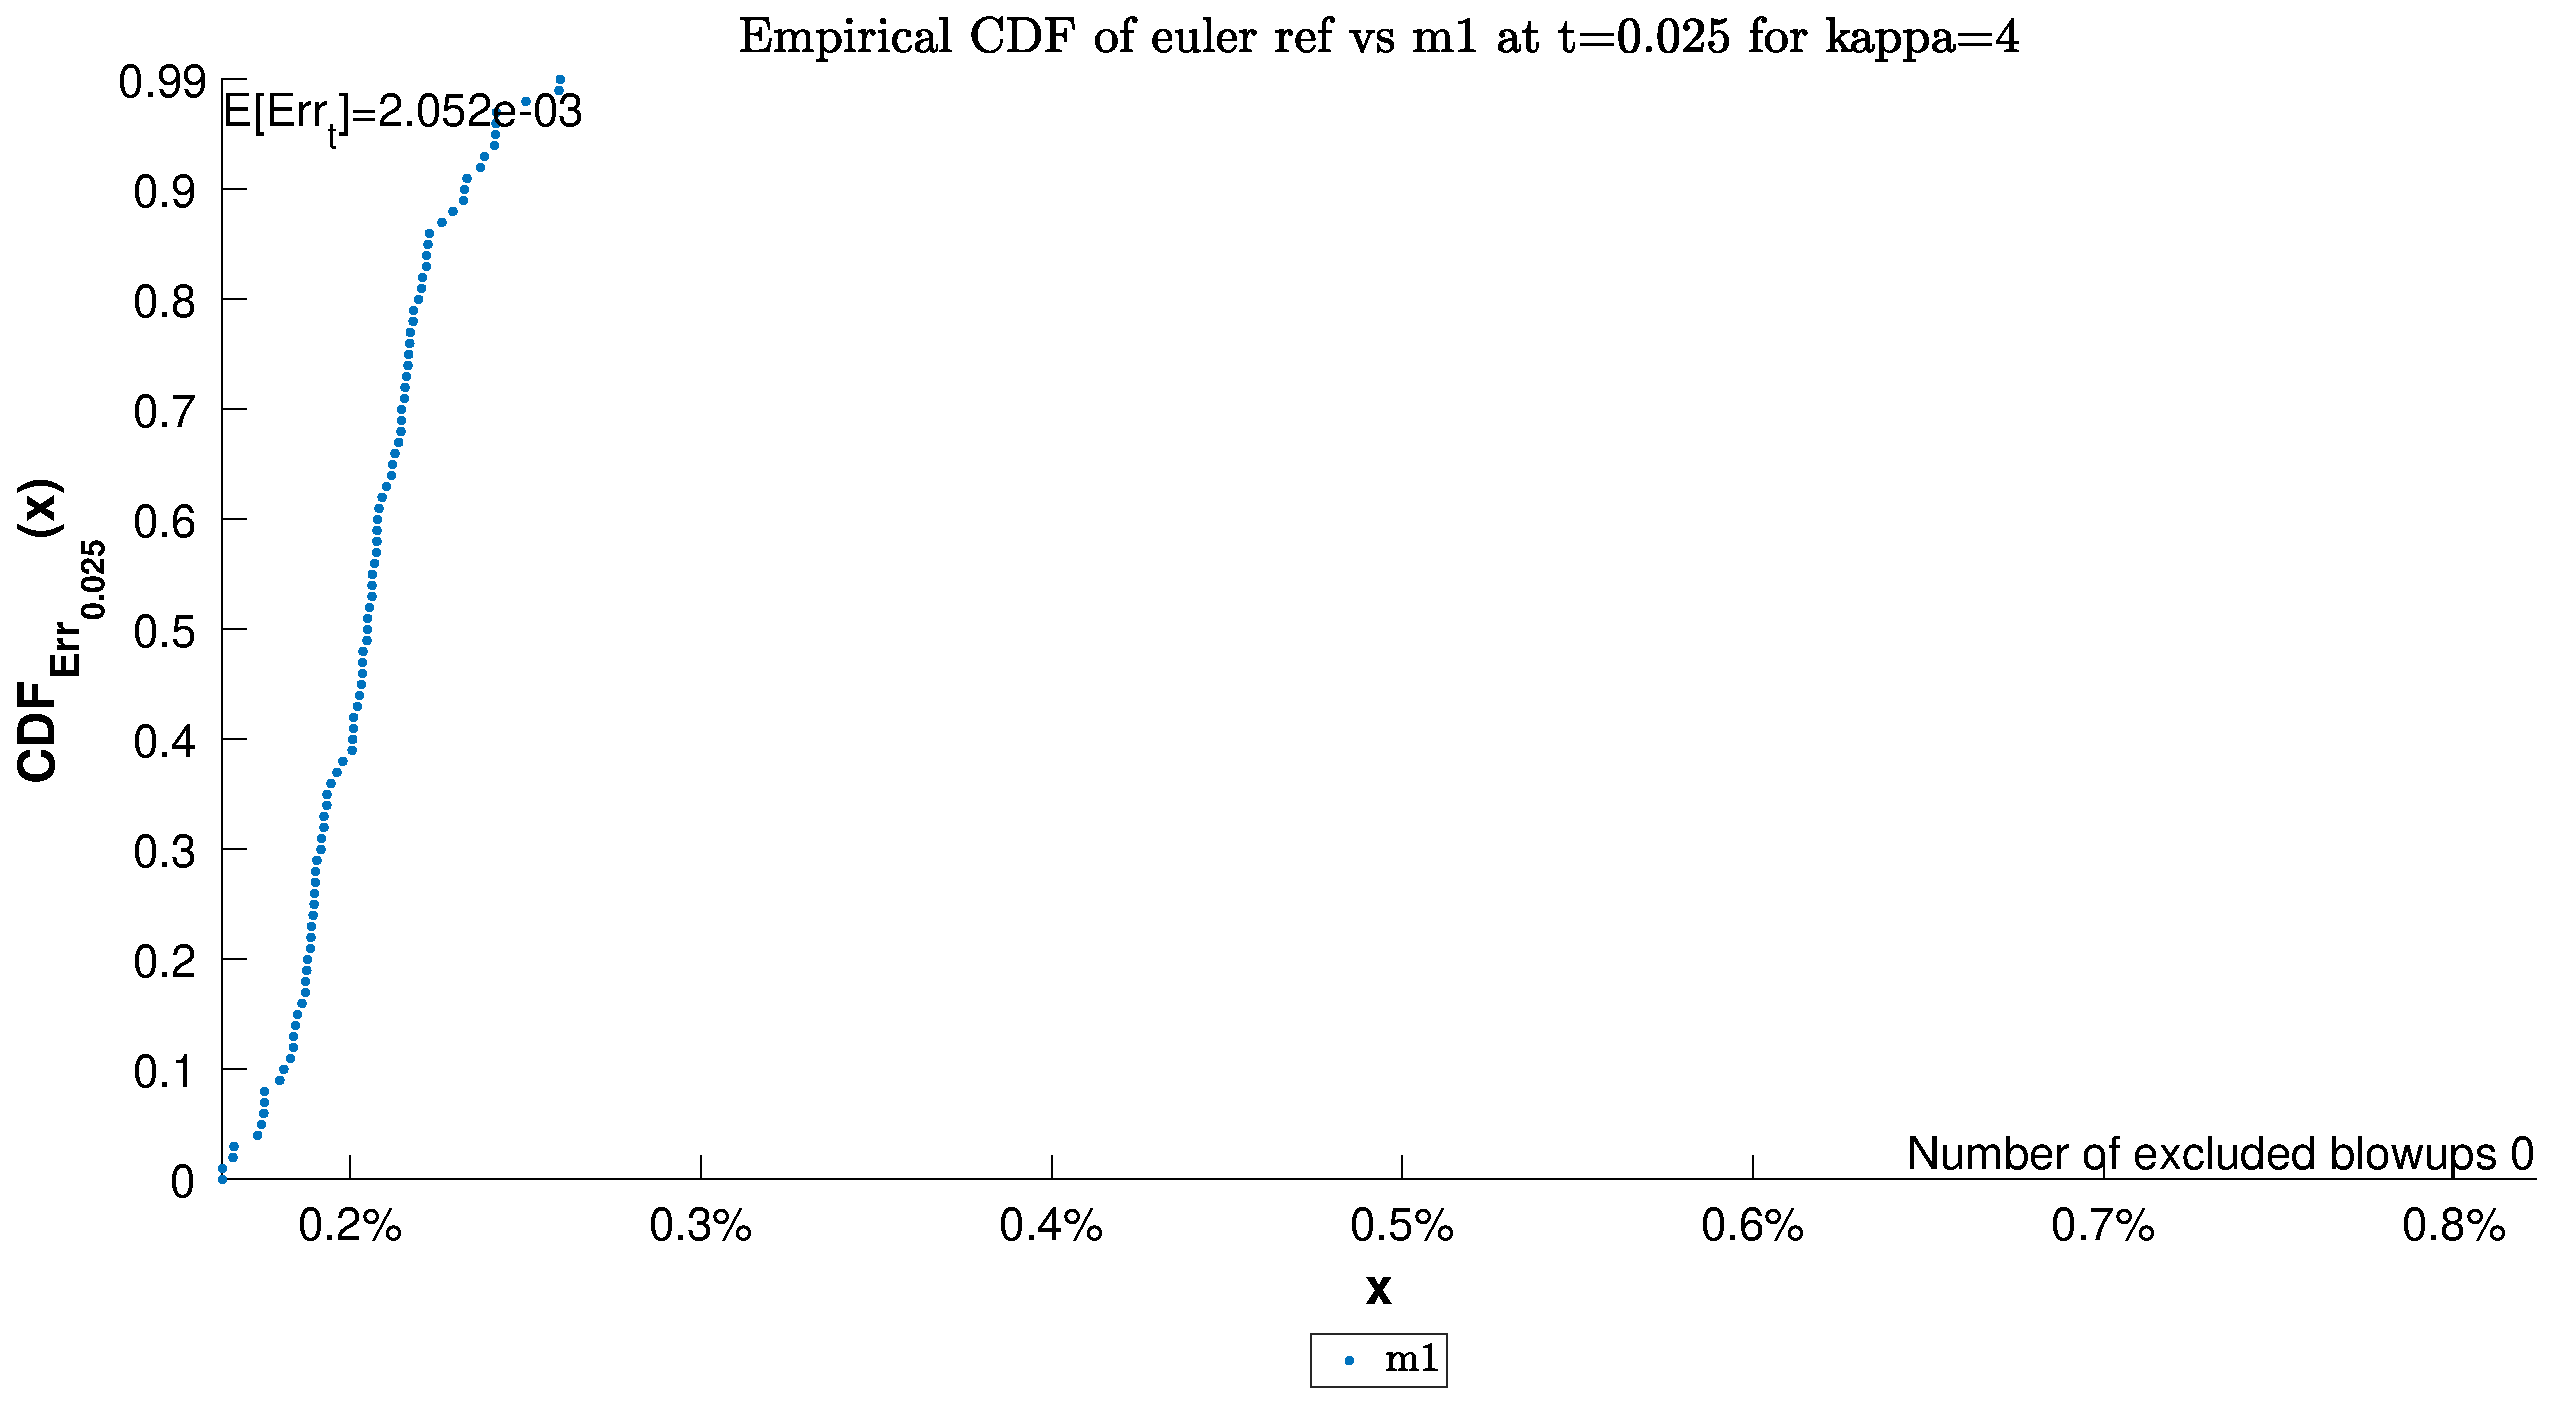
\includegraphics[width=.95\columnwidth]{CDF/CDFEulerRef_12}
\end{landscape}
\begin{landscape}
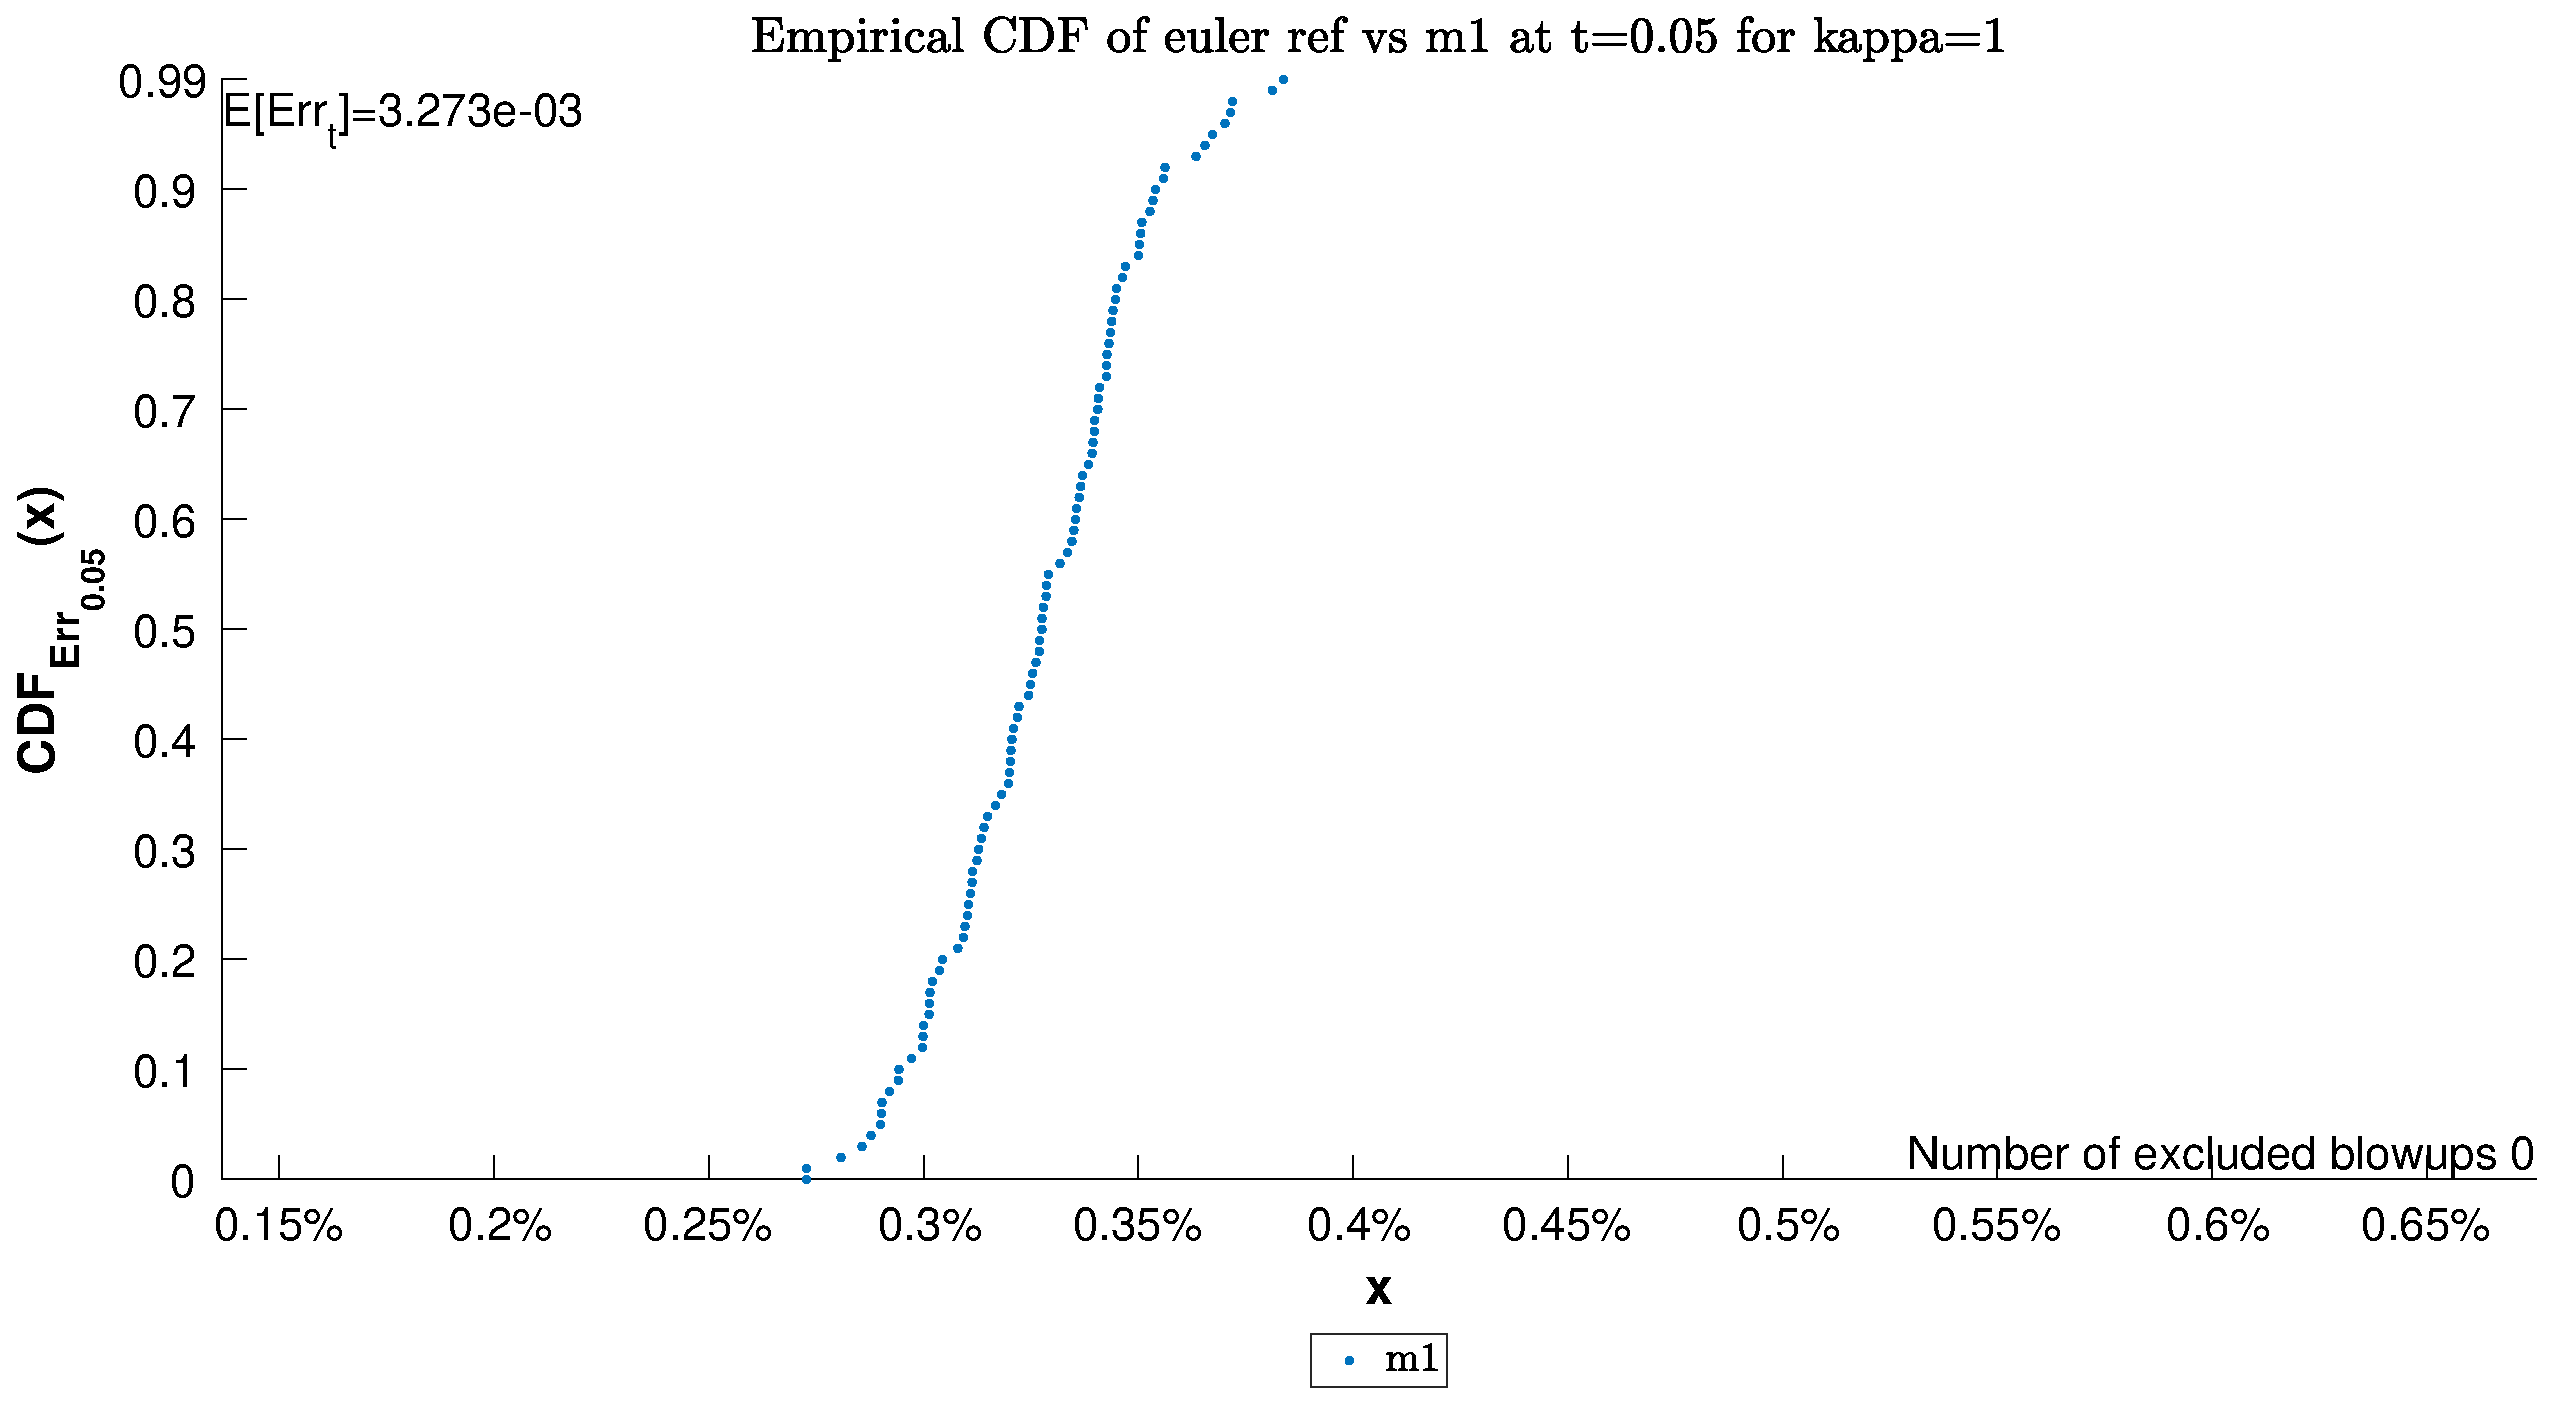
\includegraphics[width=.95\columnwidth]{CDF/CDFEulerRef_13}
\end{landscape}
\begin{landscape}
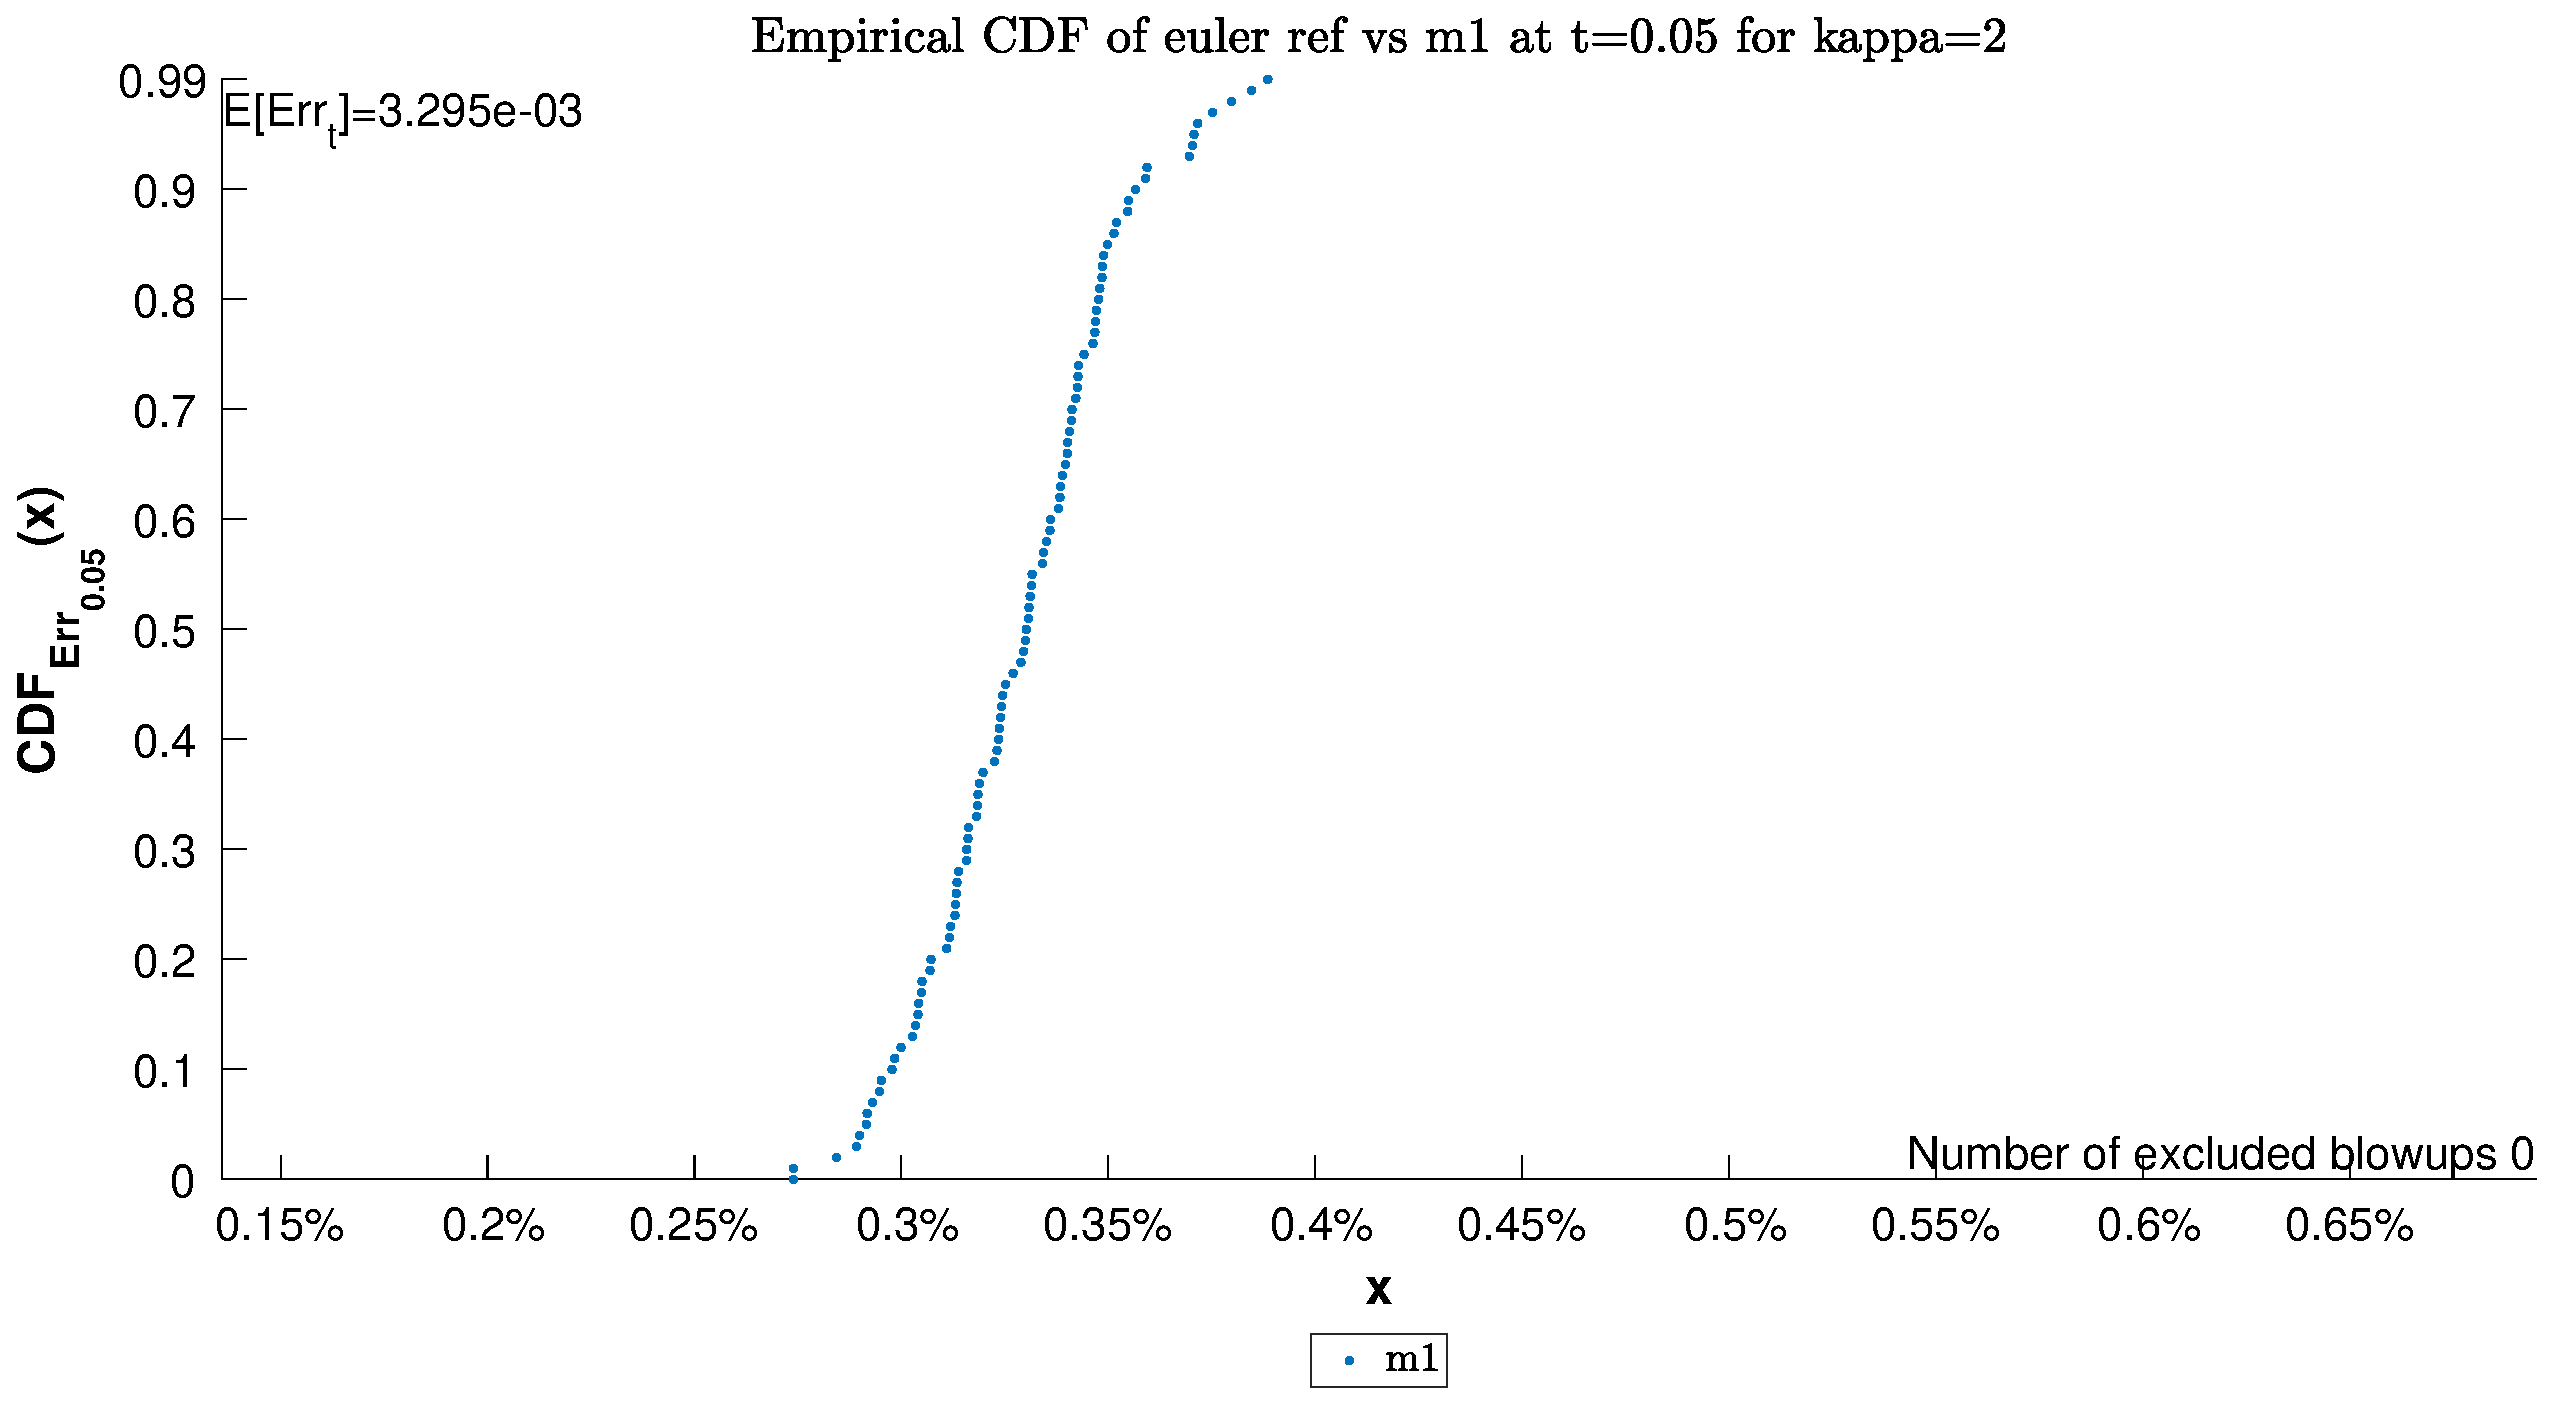
\includegraphics[width=.95\columnwidth]{CDF/CDFEulerRef_14}
\end{landscape}
\begin{landscape}
\includegraphics[width=.95\columnwidth]{CDF/CDFEulerRef_15}
\end{landscape}
\begin{landscape}
\includegraphics[width=.95\columnwidth]{CDF/CDFEulerRef_16}
\end{landscape}
\begin{landscape}
\includegraphics[width=.95\columnwidth]{CDF/CDFEulerRef_17}
\end{landscape}
\begin{landscape}
\includegraphics[width=.95\columnwidth]{CDF/CDFEulerRef_18}
\end{landscape}
\begin{landscape}
\includegraphics[width=.95\columnwidth]{CDF/CDFEulerRef_19}
\end{landscape}
\begin{landscape}
\includegraphics[width=.95\columnwidth]{CDF/CDFEulerRef_20}
\end{landscape}
\begin{landscape}
\includegraphics[width=.95\columnwidth]{CDF/CDFEulerRef_21}
\end{landscape}
\begin{landscape}
\includegraphics[width=.95\columnwidth]{CDF/CDFEulerRef_22}
\end{landscape}
\begin{landscape}
\includegraphics[width=.95\columnwidth]{CDF/CDFEulerRef_23}
\end{landscape}
\begin{landscape}
\includegraphics[width=.95\columnwidth]{CDF/CDFEulerRef_24}
\end{landscape}
\begin{landscape}
\includegraphics[width=.95\columnwidth]{CDF/CDFEulerRef_25}
\end{landscape}
\begin{landscape}
\includegraphics[width=.95\columnwidth]{CDF/CDFEulerRef_26}
\end{landscape}
\begin{landscape}
\includegraphics[width=.95\columnwidth]{CDF/CDFEulerRef_27}
\end{landscape}
\begin{landscape}
\includegraphics[width=.95\columnwidth]{CDF/CDFEulerRef_28}
\end{landscape}
\begin{landscape}
\includegraphics[width=.95\columnwidth]{CDF/CDFEulerRef_29}
\end{landscape}
\begin{landscape}
\includegraphics[width=.95\columnwidth]{CDF/CDFEulerRef_30}
\end{landscape}
\begin{landscape}
\includegraphics[width=.95\columnwidth]{CDF/CDFEulerRef_31}
\end{landscape}
\begin{landscape}
\includegraphics[width=.95\columnwidth]{CDF/CDFEulerRef_32}
\end{landscape}
\begin{landscape}
\includegraphics[width=.95\columnwidth]{CDF/CDFEulerRef_33}
\end{landscape}
\begin{landscape}
\includegraphics[width=.95\columnwidth]{CDF/CDFEulerRef_34}
\end{landscape}
\begin{landscape}
\includegraphics[width=.95\columnwidth]{CDF/CDFEulerRef_35}
\end{landscape}
\begin{landscape}
\includegraphics[width=.95\columnwidth]{CDF/CDFEulerRef_36}
\end{landscape}

